\documentclass[openany]{ctexbook}
\usepackage{anyfontsize}
\usepackage[left=3cm,right=3cm,top=3cm,bottom=3cm,headheight=13pt]{geometry}
\ctexset{
  chapter/number = \arabic{chapter},
  chapter/beforeskip = {0pt},
}
\usepackage{fancyhdr}
\fancyhf{}
\fancyhead[OC]{\kaishu\nouppercase\rightmark}
\fancyhead[OR]{\thepage}
\fancyhead[EL]{\thepage}
\fancyhead[EC]{\kaishu\nouppercase\leftmark}
\pagestyle{fancy}
\usepackage{amsmath,amssymb,amsfonts,amsthm,mathrsfs,bm}
\newtheoremstyle{kaiti}{3pt}{3pt}{\kaishu}{}{\bfseries}{}{.5em}{}
\theoremstyle{kaiti}
\newtheorem{definition}{定义}[section]
\newtheorem{theorem}{定理}[section]
\newtheorem{corollary}{推论}[section]
\newtheorem{proposition}{命题}[section]
\newtheorem{lemma}{引理}[section]
\newtheoremstyle{normal}{3pt}{3pt}{}{}{\bfseries}{}{.5em}{}
\theoremstyle{normal}
\newtheorem{example}{例}[section]
\newtheorem{remark}{注}[section]
\makeatletter
  \renewenvironment{proof}[1][\proofname]{\par
    \pushQED{\qed}%
    \normalfont \topsep6\p@\@plus6\p@\relax
    \trivlist
    \item\relax
    {\heiti #1}\hspace{2\labelsep}\ignorespaces
  }{%
    \popQED\endtrivlist\@endpefalse
  }
\makeatother
\usepackage{graphicx}
\graphicspath{{./figures/}}
\usepackage{tikz}
\usetikzlibrary{arrows.meta}
\usetikzlibrary{cd}
\tikzcdset{
  arrow style=tikz,
  diagrams={>=Latex}
}
\usepackage{subfigure}
\usepackage{longtable}
\usepackage{booktabs}
\usepackage{algorithm}
\usepackage{algorithmic}
\usepackage{hyperref}
\hypersetup{
  breaklinks,
  colorlinks = true,
  citecolor  = blue,
  linkcolor  = red,
  urlcolor   = magenta,
}

\include{macros}

\begin{document}

\title{\heiti \Huge 模式识别 \vspace{0.5cm}}
\author{\LARGE\kaishu 杨敬轩 \vspace{1cm}}

\maketitle
\thispagestyle{empty}

\frontmatter
\tableofcontents

\mainmatter
\chapter{贝叶斯决策方法}

\section{贝叶斯决策}

假设:

1. 分类数已知

2. 各类别类条件概率分布已知

先验概率:$P\left(\omega_1 \right),~P\left(\omega_2 \right)$

后验概率:
\begin{equation}
P\left(\omega_1|x \right)=\frac{P\left(\omega_1,x \right)}{P(x)}=\frac{P\left(x|\omega_1 \right)P\left(\omega_1 \right)}{\sum_iP\left(x|\omega_i \right)P\left(\omega_i \right)}
\end{equation}

贝叶斯决策:后验概率大的类
\begin{equation}
P\left(\omega_1|x \right)>P\left(\omega_2|x \right)\Rightarrow x\in \omega_1
\end{equation}

等价形式:
\begin{equation}
P\left(\omega_i|x \right)=\max_jP\left(\omega_j|x \right)\Rightarrow x\in \omega_i
\end{equation}

\section{最小错误率贝叶斯决策}

最小错误率决策:
\begin{equation}
P\left(\omega_i|x \right)=\max_jP\left(\omega_j|x \right)\Rightarrow x\in \omega_i
\end{equation}

等价形式:
\begin{equation}
P\left(x|\omega_i \right)P\left(\omega_i \right)=\max_jP\left(x|\omega_j \right)P\left(\omega_j \right)\Rightarrow x\in \omega_i
\end{equation}

似然比:
\begin{equation}
l(x)=\frac{P\left(x|\omega_1 \right)}{P\left(x|\omega_2 \right)} >\frac{P\left(\omega_2 \right)}{P\left(\omega_1 \right)} \Rightarrow x\in \omega_1
\end{equation}

负对数似然:
\begin{equation}
h(x)=-\ln \left[l(x)\right] <\ln \frac{P\left(\omega_1 \right)}{P\left(\omega_2 \right)} \Rightarrow x\in \omega_1
\end{equation}

错误率:
\begin{equation}
P\left(e \right):=\int_{-\infty}^{\infty}{p\left(e,x \right)\mathrm{d}x}=\int_{-\infty}^{\infty}{P\left(e|x \right)p(x)\mathrm{d}x}
\end{equation}

其中错误后验概率为 
\begin{equation}
P\left(e|x \right)=\min \left\{ P\left(\omega_1|x \right), P\left(\omega_2|x \right)\right\}
\end{equation}

最小错误率导出决策:
\begin{equation}
\min P\left(e \right)\Rightarrow \max P\left(\omega_i|x \right)
\end{equation}

两类错误率:使用先验概率与类条件概率密度计算
\begin{equation}
\begin{aligned}
  P\left(e \right)&=P\left(x\in \mathcal{R}_1,\omega_2 \right)+P\left(x\in \mathcal{R}_2,\omega_1 \right)\\
  &=P\left(x\in \mathcal{R}_1|\omega_2 \right)P\left(\omega_2 \right)+P\left(x\in \mathcal{R}_2|\omega_1 \right)P\left(\omega_1 \right)\\
  &=P\left(\omega_2 \right)\int_{\mathcal{R}_1}{p\left(x|\omega_2 \right)}\mathrm{d}x+P\left(\omega_1 \right)\int_{\mathcal{R}_2}{p\left(x|\omega_1 \right)}\mathrm{d}x\\
  &=P\left(\omega_2 \right)P_2\left(e \right)+P\left(\omega_1 \right)P_1\left(e \right)   
\end{aligned}
\end{equation}

\begin{figure}
  \centering
  \includegraphics[width=7cm]{1627807965262-1.2.png}
  \caption{错误率计算图示[1]}
\end{figure}

多类错误率:通过平均正确率来计算平均错误率
\begin{equation}
\begin{aligned}
  P\left(c \right)
  &=\sum_{j=1}^c{P\left(x\in \mathcal{R}_j|\omega_j \right)P\left(\omega_j \right)}\\
  &=\sum_{j=1}^c{\int_{\mathcal{R}_j}{p\left(x|\omega_j \right)P\left(\omega_j \right)}}\mathrm{d}x
\end{aligned}
\end{equation}
\begin{equation}
\begin{aligned}
  P\left(e \right)
  &=\sum_{i=1}^c{\sum_{j\ne i}{P\left(x\in \mathcal{R}_j|\omega_i \right)P\left(\omega_i \right)}}\\
  &=1-P\left(c \right)
\end{aligned}
\end{equation}

\section{最小风险贝叶斯决策}

基本思想:不同的决策错误所带来的损失可能不同

决策论表述:样本 $x\in\mathbb{R}^d$ 看做随机向量

状态空间:$c$ 个可能的状态 (类别) 
\begin{equation}
\Omega =\left\{ \omega_1,\omega_2,\dots ,\omega_c \right\}
\end{equation}

决策空间:判定样本为某类或拒绝等
\begin{equation}
\mathcal{A} =\left\{ \alpha_1,\alpha_2,\dots ,\alpha_k \right\}
\end{equation}

一般 $k\geqslant c$,
\begin{equation}
\alpha_i=\left\{ x\in \omega_i \right\} , i=1,\dots ,c
\end{equation}

$\alpha_{c+1}=\mathrm{reject}$ 等

损失函数:实际为 $\omega_j$ 类判定为 $\alpha_i$ 的损失 $\lambda \left(\alpha_i,\omega_j \right)$ →决策表

期望损失:
\begin{equation}
\begin{aligned}
  R\left(\alpha_i|x \right)
  &=\mathbb{E} \left[\lambda \left(\alpha_i,\omega_j \right)|x \right]\\
  &=\sum_j\lambda \left(\alpha_i,\omega_j \right)P\left(\omega_j|x \right)
\end{aligned}
\end{equation}

期望风险:
\begin{equation}
R\left(\alpha \right)=\int_{-\infty}^{\infty}{R\left(\alpha |x \right)p(x)}\mathrm{d}x
\end{equation}

最小风险决策:
\begin{equation}
\min R\left(\alpha \right)\Rightarrow \alpha =\mathrm{argmin}_jR\left(\alpha_j|x \right)
\end{equation}

与最小错误率决策等价:0-1 决策表
\begin{equation}
\lambda \left(\alpha_i,\omega_j \right)=1-\delta_{ij}
\end{equation}

则
\begin{equation}
\begin{aligned}
  R\left(\alpha_i|x \right)
  &=\sum_j\lambda \left(\alpha_i,\omega_j \right)P\left(\omega_j|x \right)\\
  &=\sum_{j\ne i}P\left(\omega_j|x \right)\\
  &=1-P\left(\omega_i|x \right)
\end{aligned}
\end{equation}

因此
\begin{equation}
\begin{aligned}
  \min R\left(\alpha \right)
  &\Rightarrow \min_jR\left(\alpha_j|x \right)\\
  &\Rightarrow \alpha =\mathrm{argmax}_jP\left(\omega_j|x \right)
\end{aligned}
\end{equation}

似然比:
\begin{equation}
l(x)=\frac{P\left(x|\omega_1 \right)}{P\left(x|\omega_2 \right)}>\frac{P\left(\omega_2 \right)}{P\left(\omega_1 \right)}\frac{\lambda_{12}-\lambda_{22}}{\lambda_{21}-\lambda_{11}}\Rightarrow x\in \omega_1
\end{equation}

\section{限定一类错误率条件下使另一类错误率最小}

Neyman-Pearson 决策:优化问题
\begin{equation}
\min \left\{ P_1\left(e \right)|P_2\left(e \right)-\epsilon_0=0 \right\}
\end{equation}
\begin{equation}
\begin{aligned}
  L
  &=P_1\left(e \right)+\lambda \left(P_2\left(e \right)-\epsilon_0 \right)\\
  &=\int_{\mathcal{R}_2}{p\left(x|\omega_1 \right)}\mathrm{d}x+\lambda \left(\int_{\mathcal{R}_1}{p\left(x|\omega_2 \right)}\mathrm{d}x-\epsilon_0 \right)\\
  &=1-\lambda \epsilon_o+\int_{\mathcal{R}_1}{\left[\lambda p\left(x|\omega_2 \right)-p\left(x|\omega_1 \right)\right]}\mathrm{d}x
\end{aligned}
\end{equation}

梯度条件:决策边界满足
\begin{equation}
\lambda =\frac{p\left(x|\omega_1 \right)}{p\left(x|\omega_2 \right)},~P_2\left(e \right)=\epsilon_0
\end{equation}

决策规则:
\begin{equation}
\lambda p\left(x|\omega_2 \right)-p\left(x|\omega_1 \right)<0\Rightarrow x\in \omega_1
\end{equation}

似然比:
\begin{equation}
l(x)=\frac{p\left(x|\omega_1 \right)}{p\left(x|\omega_2 \right)}>\lambda \Rightarrow x\in \omega_1
\end{equation}

对偶变量求解:通过 $l(x)$ 的映射关系,可由 $p(x)$ 求得 $p\left(l|\omega_2 \right)$,则由定义可知误差率为
\begin{equation}
\begin{aligned}
  P_2\left(e \right)
  &=1-\int_0^{\lambda}{p\left(l|\omega_2 \right)\mathrm{d}l}\\
  &=\epsilon_0\Rightarrow \lambda
\end{aligned}
\end{equation}

\section{朴素贝叶斯}

随机向量分量独立:
\begin{equation}
p\left(\vec{x}|\omega \right)=p\left(x_1,\dots ,x_d|\omega \right):=\prod_ip\left(x_i|\omega \right)
\end{equation}

\section{判别函数与正态分布}

判别函数:$g_i(x)$,例如后验概率
\begin{equation}
g_i(x)=P\left(\omega_i|x \right)
\end{equation}

取分子
\begin{equation}
g_i(x)=p\left(x|\omega_i \right)P\left(\omega_i \right)
\end{equation}

取对数
\begin{equation}
g_i(x)=\ln p\left(x|\omega_i \right)+\ln P\left(\omega_i \right)
\end{equation}

决策面方程:$g_i(x)=g_j(x)$

正态分布:
\begin{equation}
p(x)=\frac{1}{\left(2\pi \right)^{d/2}|\Sigma |^{1/2}}\exp \left\{ -\frac{1}{2}\left(x-\mu \right)^{\top}\Sigma ^{-1}\left(x-\mu \right)\right\}
\end{equation}

维数 $d$,均值 $\mu =\mathbb{E} \left[x \right]$,协方差
\begin{equation}
\Sigma =\mathbb{E} \left[\left(x-\mu \right)\left(x-\mu \right)^{\top} \right]
\end{equation}

贝叶斯判别:各类分布
\begin{equation}
p\left(x|\omega_i \right)\sim \mathcal{N} \left(\mu_i,\Sigma_i \right)
\end{equation}

则判别函数为
\begin{equation}
g_i(x)=-\frac{d}{2}\ln 2\pi -\frac{1}{2}\ln |\Sigma_i|+\ln P\left(\omega_i \right)-\frac{1}{2}\left(x-\mu_i \right)^{\top}\Sigma_{i}^{-1}\left(x-\mu_i \right)
\end{equation}

决策面方程:$g_i(x)=g_j(x)$,即
\begin{equation}
\begin{aligned}
  &-0.5\left[\left(x-\mu_i \right)^{\top}\Sigma_{i}^{-1}\left(x-\mu_i \right)-\left(x-\mu_j \right)^{\top}\Sigma_{j}^{-1}\left(x-\mu_j \right)\right]\\
  &+\left[\ln P\left(\omega_i \right)-\ln P\left(\omega_j \right)\right] -0.5\left(\ln |\Sigma_i|-\ln |\Sigma_j| \right)=0
\end{aligned}
\end{equation}

\section{分类性能评价 ROC 与 AUC}

ROC (Receiver Operating Characteristic):FP-TP 曲线,越靠近曲线左上角的点对应的阈值参数性能越好

混淆矩阵:两类分类问题

\begin{table}
  \centering
  \begin{tabular}{ccc}
    \hline
           & 实际为正类 & 实际为负类   \\ \hline
     预测为正类 & TP    & FP     \\
     预测为负类 & FN    & TN     \\ \hline
  \end{tabular}
\end{table}

AUC (Area Under ROC Curves):ROC 曲线下方面积越大越好

例:给定样本标签 
\begin{equation}
y = [1~0~1~1~1~0~0~0]
\end{equation}

分类器输出结果为
\begin{equation}
S = [0.5~0.3~0.6~0.22~0.4~0.51~0.2~0.33]
\end{equation}

则 FP 与 TP 计算如下:

\begin{table}
  \centering
  \begin{tabular}{cccc}
    \hline
    class & score & FP   & TP   \\
    \hline
    1     & 0.6   & 0    & 0.25 \\
    0     & 0.51  & 0.25 & 0.25 \\
    1     & 0.5   & 0.25 & 0.5  \\
    1     & 0.4   & 0.25 & 0.75 \\
    1     & 0.33  & 0.5  & 0.75 \\
    0     & 0.3   & 0.75 & 0.75 \\
    0     & 0.22  & 0.75 & 1    \\
    0     & 0.2   & 0.1  & 1   \\
    \hline
  \end{tabular}
\end{table}

\begin{figure}
  \centering
  \includegraphics[width=7cm]{1627808143710-1.7.png}
  \caption{ROC 曲线}
\end{figure}

\section{习题}

1. Let the conditional densities for a two-category one-dimensional problem be given by the Cauchy distribution described as follows:
\begin{equation}
  p(x|\omega_i)=\frac{1}{\pi b} \cdot \frac{1}{1+\left(\dfrac{x-a_i}{b}\right)^2},\quad  i=1,2.
\end{equation}

1.1. By explicit integration, check that the distributions are indeed normalized.

解: 直接积分可得, $\forall~i=1,2$, 有
\begin{equation}
  \begin{aligned}
    \int_{-\infty}^{\infty}p(x|\omega_i)\mathrm{d}x
    &=\int_{-\infty}^{\infty}\frac{1}{\pi b} \cdot \frac{1}{1+\left(\dfrac{x-a_i}{b}\right)^2}\mathrm{d}x \\
    &=\frac{1}{\pi}\int_{-\infty}^{\infty}\frac{1}{1+u^2}\mathrm{d}u,\quad u=\frac{x-a_i}{b} \\
    &=\frac{1}{\pi}\arctan(u)\Big|_{-\infty}^{\infty} \\
    &=\frac{1}{\pi}\left(\frac{\pi}{2}+\frac{\pi}{2}\right)\\
    &=1\\
  \end{aligned}
\end{equation}

故此分布函数是归一化的.

1.2. Assuming $P(\omega_1) = P(\omega_2)$, show that $P(\omega_1|x)=P(\omega_2|x)$ if $x=(a_1+a_2)/2$, i.e., the minimum error decision boundary is a point midway between the peaks of the two distributions, regardless of $b$.

解: 由 Bayes 公式可知
\begin{equation}
  P(\omega_1|x)=\frac{p(x|\omega_1)P(\omega_1)}{p(x)}
\end{equation}
\begin{equation}
  P(\omega_2|x)=\frac{p(x|\omega_2)P(\omega_2)}{p(x)}
\end{equation}

令 $P(\omega_1|x)=P(\omega_2|x)$ 可得
\begin{equation}
  \frac{p(x|\omega_1)P(\omega_1)}{p(x)}=\frac{p(x|\omega_2)P(\omega_2)}{p(x)}
\end{equation}

又 $P(\omega_1) = P(\omega_2)$, 则
\begin{equation}
  p(x|\omega_1)=p(x|\omega_2)
\end{equation}

即
\begin{equation}
  \frac{1}{\pi b} \cdot \frac{1}{1+\left(\dfrac{x-a_1}{b}\right)^2}=\frac{1}{\pi b} \cdot \frac{1}{1+\left(\dfrac{x-a_2}{b}\right)^2}
\end{equation}

整理得
\begin{equation}
  |x-a_1|=|x-a_2|
\end{equation}

易知 $x=(a_1+a_2)/2$ 满足上式.

1.3. Assuming $P(\omega_1) = P(\omega_2)$, plot $P(\omega_1|x)$ for the case $a_1=3$, $a_2=5$ and $b=1$.

解: 由 Bayes 公式可得
\begin{equation}
  \begin{aligned}
    P(\omega_1|x)
    &=\frac{p(x|\omega_1)P(\omega_1)}{p(x)}\\
    &=\frac{p(x|\omega_1)P(\omega_1)}{p(x|\omega_1)P(\omega_1)+p(x|\omega_2)P(\omega_2)}\\
    &=\frac{p(x|\omega_1)}{p(x|\omega_1)+p(x|\omega_2)}\\
    &=\frac{\dfrac{1}{\pi b} \cdot \dfrac{1}{1+\left(\dfrac{x-a_1}{b}\right)^2}}{\dfrac{1}{\pi b} \cdot \dfrac{1}{1+\left(\dfrac{x-a_1}{b}\right)^2}+\dfrac{1}{\pi b} \cdot \dfrac{1}{1+\left(\dfrac{x-a_2}{b}\right)^2}}\\
    &=\frac{1+\left(\dfrac{x-a_2}{b}\right)^2}{1+\left(\dfrac{x-a_1}{b}\right)^2+1+\left(\dfrac{x-a_2}{b}\right)^2}
  \end{aligned}
  \label{eq:postpdf}
\end{equation}

易知
\begin{equation}
  P(\omega_2|x)=1-P(\omega_1|x)
\end{equation}

代入已知数值可绘图如图 \ref{fig:postpdf} 所示.

\begin{figure}
  \centering
  \includegraphics[width=10cm]{postpdf.pdf}
  \caption{后验概率}
  \label{fig:postpdf}
\end{figure}

1.4. Assuming $P(\omega_1) = P(\omega_2)$, how do $P(\omega_1|x)$ and $P(\omega_2|x)$ behave as $x \rightarrow -\infty$? $x\rightarrow +\infty$? Explain.

解: 由图 \ref{fig:postpdf} 可知, 当 $x \rightarrow \pm\infty$ 时, $P(\omega_1|x)=P(\omega_2|x)=\dfrac{1}{2}$, 证明如下.

对式 (\ref{eq:postpdf}) 取极限可得
\begin{equation}
  \lim_{x\to\pm\infty}P(\omega_1|x)
  =\lim_{x\to\pm\infty}\frac{1+\left(\dfrac{x-a_2}{b}\right)^2}{1+\left(\dfrac{x-a_1}{b}\right)^2+1+\left(\dfrac{x-a_2}{b}\right)^2}=\frac{1}{2}
\end{equation}

则有
\begin{equation}
  \lim_{x\to\pm\infty}P(\omega_2|x)
  =\frac{1}{2}
\end{equation}

2. Consider Neyman-Pearson criteria for two Cauchy distributions in one dimension described in Problem 1. Assume a zero-one error loss, and for simplicity $a_{2}>a_{1}$, the same ``width" $b$, and equal priors.

2.1. Suppose the maximum acceptable error rate for classifying a pattern that is actually in $\omega_{1}$ as if it were in $\omega_{2}$ is $E_{1}$. Determine the decision boundary in terms of the variables given.

解: 本题要求考虑 Neyman-Pearson 准则, 则边界并不一定是单边边界, 以下为大部分错误解法. 

设边界点为 $t$, 由 $a_{2}>a_{1}$ 可知
\begin{equation}
  R_1=(-\infty,t),\quad R_2=(t,\infty)
\end{equation}

又先验概率相等, 则
\begin{equation}
  P(\omega_1)=p(\omega_2)=\frac{1}{2}
\end{equation}

故第一类错误率
\begin{equation}
  \begin{aligned}
    E_1
    &=\int_t^\infty p(x|\omega_1)P(\omega_1)\mathrm{d}x\\
    &=\frac{1}{2}\int_t^\infty \frac{1}{\pi b} \cdot \frac{1}{1+\left(\dfrac{x-a_1}{b}\right)^2}\mathrm{d}x\\
    &=\frac{1}{2\pi}\int_{(t-a_1)/b}^\infty \frac{1}{1+u^2}\mathrm{d}u,\quad u=\dfrac{x-a_1}{b}\\
    &=\frac{1}{2\pi}\arctan(u)\Big|_{(t-a_1)/b}^\infty\\
    &=\frac{1}{2\pi}\left[\frac{\pi}{2}-\arctan\left(\frac{t-a_1}{b}\right)\right]
  \end{aligned}
\end{equation}

即
\begin{equation}
  \arctan\left(\frac{t-a_1}{b}\right)=\frac{\pi}{2}-2\pi E_1
\end{equation}

两边取正切可得
\begin{equation}
  \frac{t-a_1}{b}=\tan\left(\frac{\pi}{2}-2\pi E_1\right)=\cot(2\pi E_1)
\end{equation}

故
\begin{equation}
  t=a_1+b\cot(2\pi E_1)=a_1+\frac{b}{\tan(2\pi E_1)}
\end{equation}

正确解法应为, 考虑两类错误
\begin{equation}
  \begin{aligned}
    P_1(e)&=\int_{\Rc_2}p(x|\omega_1)\mathrm{d}x=E_1\\
    P_2(e)&=\int_{\Rc_1}p(x|\omega_2)\mathrm{d}x\\
  \end{aligned}
\end{equation}

最小化 $P_2(e)$ 等价于
\begin{equation}
  \min\gamma=P_2(e)+\lambda(P_1(e)-E_1)
\end{equation}

对 $\lambda$ 和 $\Rc_2$ 边界求导等于 0, 有
\begin{equation}
    \lambda=\frac{p(x|\omega_2)}{p(x|\omega_1)}=\frac{b^2+(x-a_1)^2}{b^2+(x-a_2)^2}
\end{equation}
\begin{equation}
  \int_{\Rc_2}p(x|\omega_1)\mathrm{d}x=E_1
\end{equation}

则决策边界为
\begin{equation}
  t_{1,2}=\frac{(a_1-\lambda a_2)\pm\sqrt{\lambda(a_1-a_2)^2-b^2(\lambda-1)^2}}{1-\lambda}
\end{equation}

2.2. For this boundary, what is the error rate for classifying $\omega_{2}$ as $\omega_{1}$?

解: 第二类错误率为
\begin{equation}
  \begin{aligned}
    E_2
    &=\int_{-\infty}^{\top} p(x|\omega_2)P(\omega_2)\mathrm{d}x\\
    &=\frac{1}{2}\int_{-\infty}^{\top}\frac{1}{\pi b} \cdot \frac{1}{1+\left(\dfrac{x-a_2}{b}\right)^2}\mathrm{d}x\\
    &=\frac{1}{2\pi}\int_{-\infty}^{(t-a_2)/b}\frac{1}{1+u^2}\mathrm{d}u\\
    &=\frac{1}{2\pi}\left[\arctan\left(\frac{t-a_2}{b}\right)+\frac{\pi}{2}\right]
  \end{aligned}
\end{equation}

2.3. What is the overall error rate under zero-one loss?

解: 总错误率为
\begin{equation}
  E=E_1+E_2=E_1+\frac{1}{2\pi}\left[\arctan\left(\frac{t-a_2}{b}\right)+\frac{\pi}{2}\right]
\end{equation}

2.4. Apply your results to the specific case $b=1$ and $a_{1}=-1, a_{2}=1$ and $E_{1}=0.1$.

解: 代入数值得边界点为
\begin{equation}
  t=a_1+\frac{b}{\tan(2\pi E_1)}=-1+\frac{1}{\tan(2\pi\times0.1)}\approx0.376
\end{equation}

则总错误率为
\begin{equation}
  \begin{aligned}
    E
    &=E_1+\frac{1}{2\pi}\left[\arctan\left(\frac{t-a_2}{b}\right)+\frac{\pi}{2}\right]\\
    &=0.1+\frac{1}{2\pi}\left[\arctan\left(\frac{0.376-1}{1}\right)+\frac{\pi}{2}\right]\\
    &\approx0.261\\
  \end{aligned}
\end{equation}

2.5. Compare your result to the Bayes error rate (i.e. without the Neyman-Pearson conditions).

解: 对于 Bayes 决策, 分界点为
\begin{equation}
  t=\frac{a_1+a_2}{2}=\frac{-1+1}{2}=0
\end{equation}

故 Bayes 错误率为
\begin{equation}
  \begin{aligned}
    E_B
    &=\int_{-\infty}^{\top} p(x|\omega_2)P(\omega_2)\mathrm{d}x+\int_t^\infty p(x|\omega_1)P(\omega_1)\mathrm{d}x\\
    &=\frac{1}{2\pi}\left[\frac{\pi}{2}-\arctan\left(\frac{t-a_1}{b}\right)\right]+\frac{1}{2\pi}\left[\arctan\left(\frac{t-a_2}{b}\right)+\frac{\pi}{2}\right]\\
    &=\frac{1}{2}-\frac{1}{2\pi}\arctan\left(\frac{0+1}{1}\right)+\frac{1}{2\pi}\arctan\left(\frac{0-1}{1}\right)\\
    &=\frac{1}{4}\\
  \end{aligned}
\end{equation}

由 $E_B<E$ 可知 Bayes 决策错误率小于 Neyman-Pearson 决策错误率.

3. In many pattern classification problems one has the option either to assign the pattern to one of $c$ classes, or to \emph{reject} it as being unrecognizable. If the cost for rejects is not too high, rejection may be a desirable action. Let
\begin{equation}
  \lambda(\alpha_i|\omega_j)=
  \left\{
    \begin{array}{ll}
    0         & i=j, \quad i,j=1,2,\cdots, c  \\
    \lambda_r & i = c+1 \\
    \lambda_s & \mathrm{otherwise},  
    \end{array}
  \right.
\end{equation}

where $\lambda_r$ is the loss incurred for choosing the $(c+1)$th action, rejection, and $\lambda_s$ is the loss incurred for making a substitution error. Show that the minimum risk is obtained if we decide $\omega_i$ if $P(\omega_i|\bm{x})\gs P(\omega_j|\bm{x})$ for all $j$ and if $P(\omega_i|\bm{x})\gs 1-\lambda_r/\lambda_s$, and reject otherwise. What happens if $\lambda_r=0$? What happens if $\lambda_r>\lambda_s$?

解: 令
\begin{equation}
  m=\argmax_{j=1,2,\cdots,c}P(\omega_j|x)
\end{equation}

即 $\omega_m$ 表示后验概率最大的类别, 分类讨论. 

当选择 $\omega_m$ 时, 风险为
\begin{equation}
  R_m=\lambda_s\sum_{j\neq m}P(\omega_j|x)=\lambda_s[1-P(\omega_m|x)]
\end{equation}

当选择其他类别 $\omega_k$, $k\neq m$ 时, 风险为
\begin{equation}
  R_k=\lambda_s\sum_{j\neq k}P(\omega_j|x)=\lambda_s[1-P(\omega_k|x)]\gs\lambda_s[1-P(\omega_m|x)]
\end{equation}

当选择拒绝时, 风险为
\begin{equation}
  R_r=\lambda_r
\end{equation}

所以最小风险为
\begin{equation}
  \begin{aligned}
    R
    &=\min\{R_m,R_k,R_r\}\\
    &=\min\{\lambda_s[1-P(\omega_m|x)],\lambda_r\}\\
  \end{aligned}
\end{equation}

当 $\lambda_s[1-P(\omega_m|x)]\ls\lambda_r$, 即
\begin{equation}
  P(\omega_m|x)\gs1-\frac{\lambda_r}{\lambda_s}
\end{equation}

时, 选择 $\omega_m$ 风险最小, 否则选择拒绝风险最小.

若 $\lambda_r=0$, 则选择拒绝风险最小, 会拒绝所有样本.

若 $\lambda_r>\lambda_s$, 则选择最大后验概率类别 $\omega_m$ 风险最小, 不会拒绝任何样本.

4. Consider a two-category classification problem in two dimensions. Given the following conditions, calculate the Bayes decision boundary respectively and plot them in the coordinate space (with computer or by hand). You should indicate the mean point of each category.

4.1. We set $p(\bm{x}|\omega_1)\sim N(\bm{0},\bm{I})$, $p(\bm{x}|\omega_2)\sim N\left((1,1)^{\top},\bm{I}\right)$ and $P(\omega_1)=P(\omega_2)=0.5$. 

解: 忽略类别无关项, 判别函数为
\begin{equation}
  g_i(\vx)=-\frac{1}{2\sigma^2}(\vx-\vmu_i)^{\top}(\vx-\vmu_i)
\end{equation}

决策面满足
\begin{equation}
  g_i(\vx)=g_j(\vx)
\end{equation}

故
\begin{equation}
  -\frac{1}{2\sigma^2}(\vx-\vmu_i)^{\top}(\vx-\vmu_i)=-\frac{1}{2\sigma^2}(\vx-\vmu_j)^{\top}(\vx-\vmu_j)
\end{equation}

化简得
\begin{equation}
  -2\vx^{\top}\vmu_i+\vmu_i^{\top}\vmu_i=-2\vx^{\top}\vmu_j+\vmu_j^{\top}\vmu_j
\end{equation}

即
\begin{equation}
  (\vmu_i-\vmu_j)^{\top}\vx-\frac{1}{2}(\vmu_i^{\top}\vmu_i-\vmu_j^{\top}\vmu_j)=0
\end{equation}

代入数据得
\begin{equation}
  x_1+x_2-1=0
\end{equation}

决策面如图 \ref{fig:mvnpdf-1} 所示.

\begin{figure}
  \centering
  \includegraphics[width=10cm]{mvnpdf-1.pdf}
  \caption{决策面}
  \label{fig:mvnpdf-1}
\end{figure}

4.2. We set $p(\bm{x}|\omega_1)\sim N(\bm{0},\bm{I})$, $p(\bm{x}|\omega_2)\sim N\left((1,1)^{\top},\bm{I}\right)$ and $P(\omega_1)=0.2, P(\omega_2)=0.8$.

解: 忽略类别无关项, 判别函数为
\begin{equation}
  g_i(\vx)=-\frac{1}{2\sigma^2}(\vx-\vmu_i)^{\top}(\vx-\vmu_i)+\ln P(\omega_i)
\end{equation}

决策面满足
\begin{equation}
  g_i(\vx)=g_j(\vx)
\end{equation}

故
\begin{equation}
  -\frac{1}{2\sigma^2}(\vx-\vmu_i)^{\top}(\vx-\vmu_i)+\ln P(\omega_i)=-\frac{1}{2\sigma^2}(\vx-\vmu_j)^{\top}(\vx-\vmu_j)+\ln P(\omega_j)
\end{equation}

化简得
\begin{equation}
  -2\vx^{\top}\vmu_i+\vmu_i^{\top}\vmu_i-2\sigma^2\ln P(\omega_i)
  =-2\vx^{\top}\vmu_j+\vmu_j^{\top}\vmu_j-2\sigma^2\ln P(\omega_j)
\end{equation}

即
\begin{equation}
  (\vmu_i-\vmu_j)^{\top}\vx-\frac{1}{2}(\vmu_i^{\top}\vmu_i-\vmu_j^{\top}\vmu_j)+\sigma^2\ln\frac{P(\omega_i)}{P(\omega_j)}=0
\end{equation}

代入数据得
\begin{equation}
  x_1+x_2-1+\ln4=0
\end{equation}

决策面如图 \ref{fig:mvnpdf-2} 所示.

\begin{figure}
  \centering
  \includegraphics[width=10cm]{mvnpdf-2.pdf}
  \caption{决策面}
  \label{fig:mvnpdf-2}
\end{figure}

4.3. We set $p(\bm{x}|\omega_1)\sim N\left(\bm{0},\begin{bmatrix} 1 & 1 \\ 1 & 2 \end{bmatrix}\right)$, $p(\bm{x}|\omega_2)\sim N\left((1,1)^{\top},\begin{bmatrix} 1 & 1 \\ 1 & 2 \end{bmatrix}\right)$ and $P(\omega_1)=P(\omega_2)=0.5$.

解: 忽略类别无关项, 判别函数为
\begin{equation}
  g_i(\vx)=-\frac{1}{2}(\vx-\vmu_i)^{\top}\mSigma^{-1}(\vx-\vmu_i)
\end{equation}

决策面满足
\begin{equation}
  g_i(\vx)=g_j(\vx)
\end{equation}

故
\begin{equation}
  -\frac{1}{2}(\vx-\vmu_i)^{\top}\mSigma^{-1}(\vx-\vmu_i)=-\frac{1}{2}(\vx-\vmu_j)^{\top}\mSigma^{-1}(\vx-\vmu_j)
\end{equation}

化简得
\begin{equation}
  -2\vx^{\top}\mSigma^{-1}\vmu_i+\vmu_i^{\top}\mSigma^{-1}\vmu_i
  =-2\vx^{\top}\mSigma^{-1}\vmu_j+\vmu_j^{\top}\mSigma^{-1}\vmu_j
\end{equation}

即
\begin{equation}
  (\vmu_i-\vmu_j)^{\top}\mSigma^{-1}\vx-\frac{1}{2}(\vmu_i^{\top}\mSigma^{-1}\vmu_i-\vmu_j^{\top}\mSigma^{-1}\vmu_j)=0
\end{equation}

代入数据得
\begin{equation}
  x_1-\frac{1}{2}=0
\end{equation}

决策面如图 \ref{fig:mvnpdf-3} 所示.

\begin{figure}
  \centering
  \includegraphics[width=10cm]{mvnpdf-3.pdf}
  \caption{决策面}
  \label{fig:mvnpdf-3}
\end{figure}

4.4. We set $p(\bm{x}|\omega_1)\sim N\left(\bm{0},\begin{bmatrix} 1 & 0 \\ 0 & 2 \end{bmatrix}\right)$, $p(\bm{x}|\omega_2)\sim N\left((1,1)^{\top},\begin{bmatrix} 2 & 0 \\ 0 & 1 \end{bmatrix}\right)$ and $P(\omega_1)=P(\omega_2)=0.5$.

解: 忽略类别无关项, 判别函数为
\begin{equation}
  g_i(\vx)=-\frac{1}{2}(\vx-\vmu_i)^{\top}\mSigma_i^{-1}(\vx-\vmu_i)-\frac{1}{2}\ln|\mSigma_i|
\end{equation}

决策面满足
\begin{equation}
  g_i(\vx)=g_j(\vx)
\end{equation}

故
\begin{equation}
  -\frac{1}{2}(\vx-\vmu_i)^{\top}\mSigma_i^{-1}(\vx-\vmu_i)-\frac{1}{2}\ln|\mSigma_i|=-\frac{1}{2}(\vx-\vmu_j)^{\top}\mSigma_j^{-1}(\vx-\vmu_j)-\frac{1}{2}\ln|\mSigma_j|
\end{equation}

化简得
\begin{equation}
  \vx^{\top}\mSigma_i^{-1}\vx-2\vx^{\top}\mSigma_i^{-1}\vmu_i+\vmu_i^{\top}\mSigma_i^{-1}\vmu_i+\ln|\mSigma_i|
  =\vx^{\top}\mSigma_j^{-1}\vx-2\vx^{\top}\mSigma_j^{-1}\vmu_j+\vmu_j^{\top}\mSigma_j^{-1}\vmu_j+\ln|\mSigma_j|
\end{equation}

即
\begin{equation}
  \vx^{\top}(\mSigma_j^{-1}-\mSigma_i^{-1})\vx+2(\vmu_i\mSigma_i^{-1}-\vmu_j\mSigma_j^{-1})^{\top}\vx-(\vmu_i^{\top}\mSigma_i^{-1}\vmu_i-\vmu_j^{\top}\mSigma_j^{-1}\vmu_j)-(\ln|\mSigma_i|-\ln|\mSigma_j|)=0
\end{equation}

代入数据得
\begin{equation}
  \frac{1}{2}x_1^2-\frac{1}{2}x_2^2+x_1+2x_2-\frac{3}{2}=0
\end{equation}

化简得
\begin{equation}
  x_1^2-x_2^2+2x_1+4x_2-3=0
\end{equation}

即
\begin{equation}
  (x_1+1)^2-(x_2-2)^2=0
\end{equation}

即
\begin{equation}
  |x_1+1|=|x_2-2|
\end{equation}

决策面如图 \ref{fig:mvnpdf-4} 所示.

\begin{figure}[t]
  \centering
  \includegraphics[width=10cm]{mvnpdf-4.pdf}
  \caption{决策面}
  \label{fig:mvnpdf-4}
\end{figure}

5. Consider a simple learning problem of determining whether Alice and Bob from CA will go to hiking or not, $Y:Hike\in\{T,F\}$ given the weather conditions $X_1:Sunny\in\{T,F\}$ and $X_2:Windy\in\{T,F\}$ by a Naive Bayes classifier. Using training data, we estimated the parameters $P(Hike) = 0.5$, $P(Sunny|Hike) = 0.9$, $P(Windy|\neg Hike) = 0.8$, $P(Windy|Hike) = 0.3$ and $P(Sunny|\neg Hike) = 0.4$. Assume that the true distributions of $X_1$, $X_2$, and $Y$ satisfy the Naive Bayes assumption of conditional independence with the above parameters.

5.1. Assume Sunny and Windy are truly independent given Hike. Write down the Naive Bayes decision rule for this problem using both attributes Sunny and Windy.

解: 已知 $P(Hike) = 0.5$, 则 $P(\neg Hike)=P(Hike)=0.5$. 

由 Bayes 公式结合条件独立的假设可得
\begin{equation}
  \begin{aligned}
    P(Hike|Sunny,Windy)&=\frac{0.9\times0.3}{0.9\times0.3+0.4\times0.8}=0.4576\\
    P(Hike|Sunny,\neg Windy)&=\frac{0.9\times0.7}{0.9\times0.7+0.4\times0.2}=0.8873\\
    P(Hike|\neg Sunny,Windy)&=\frac{0.1\times0.3}{0.1\times0.3+0.6\times0.8}=0.0588\\
    P(Hike|\neg Sunny,\neg Windy)&=\frac{0.1\times0.7}{0.1\times0.7+0.6\times0.2}=0.3684\\
  \end{aligned}
\end{equation}

所以
\begin{equation}
  \begin{aligned}
    P(Hike|Sunny,Windy)&<P(\neg Hike|Sunny,Windy)\\
    P(Hike|Sunny,\neg Windy)&>P(\neg Hike|Sunny,\neg Windy)\\
    P(Hike|\neg Sunny,Windy)&<P(\neg Hike|\neg Sunny,Windy)\\
    P(Hike|\neg Sunny,\neg Windy)&<P(\neg Hike|\neg Sunny,\neg Windy)\\
  \end{aligned}
\end{equation}

因此 Bayes 决策规则为
\begin{equation}
  \begin{aligned}
    (Sunny,Windy)&\to\neg Hike\\
    (Sunny,\neg Windy)&\to Hike\\
    (\neg Sunny,Windy)&\to\neg Hike\\
    (\neg Sunny,\neg Windy)&\to\neg Hike\\
  \end{aligned}
\end{equation}

5.2. Given the decision rule above, what is the expected error rate of the Naive Bayes classifier? (The expected error rate is the probability that each class generates an observation where the decision rule is incorrect.)

解: 由 Bayes 决策规则可知, 错误率为
\begin{equation}
  \begin{aligned}
    E
    &=P(Hike)[1-P(Sunny,\neg Windy|Hike)]+P(\neg Hike)P(Sunny,\neg Windy|\neg Hike)\\
    &=0.5\times(1-0.9\times0.7)+0.5\times0.4\times0.2\\
    &=0.225\\
  \end{aligned}
\end{equation}

5.3. What is the joint probability that Alice and Bob go to hiking and the weather is sunny and windy, that is $P(Sunny,Windy,Hike)$?

解: 由条件乘法公式与条件独立性可知, 联合概率密度为
\begin{equation}
  \begin{aligned}
    P(Sunny,Windy,Hike)
    &=P(Hike)P(Sunny,Windy|Hike)\\
    &=P(Hike)P(Sunny|Hike)P(Windy|Hike)\\
    &=0.5 \times 0.9 \times 0.3\\
    &=0.135\\
  \end{aligned}
\end{equation}

5.4. Next, suppose that we gather more information about weather conditions and introduce a new feature denoting whether the weather is $X_3$: Rainy or not. Assume that each day the weather in CA can be either Rainy or Sunny. That is, it can not be both Sunny and Rainy (similarly, it can not be $\neg Sunny$ and $\neg Rainy$). In the above new case, are any of the Naive Bayes assumptions violated? Why (not)? What is the joint probability that Alice and Bob go to hiking and the weather is sunny, windy and not rainy, that is $P(Sunny,Windy,\neg Rainy,Hike)$?

解: 确有 Naive Bayes 的假设不成立, 事实上
\begin{equation}
  P(Sunny,Windy,Rainy|Hike)=0
\end{equation}

而
\begin{equation}
  \begin{aligned}
     &~P(Sunny|Hike)P(Windy|Hike)P(Rainy|Hike)\\
    =&~P(Sunny|Hike)P(Windy|Hike)P(\neg Sunny|Hike)\\
    =&~0.9\times0.3\times0.1\\
    =&~0.027\\
  \end{aligned}
\end{equation}

所以
\begin{equation}
  P(Sunny,Windy,Rainy|Hike)\neq P(Sunny|Hike)P(Windy|Hike)P(Rainy|Hike)
\end{equation}

故 Naive Bayes 的条件独立性假设不成立.

由题干假设以及条件乘法公式可知, 联合概率密度为
\begin{equation}
  \begin{aligned}
    P(Sunny,Windy,\neg Rainy,Hike)
    &=P(Sunny,Windy,Hike)\\
    &=P(Hike)P(Sunny,Windy|Hike)\\
    &=P(Hike)P(Sunny|Hike)P(Windy|Hike)\\
    &=0.5 \times 0.9 \times 0.3\\
    &=0.135\\
  \end{aligned}
\end{equation}


5.5. What is the expected error rate when the Naive Bayes classier uses all three attributes? Will the performance of Naive Bayes be improved by observing the new attribute Rainy? Explain why. 

解: 考虑三种因素的 Bayes 决策规则为
\begin{equation}
  \begin{aligned}
    (Sunny,Windy,\neg Rainy)&\to\neg Hike\\
    (Sunny,\neg Windy,\neg Rainy)&\to Hike\\
    (\neg Sunny,Windy,Rainy)&\to\neg Hike\\
    (\neg Sunny,\neg Windy,Rainy)&\to\neg Hike\\
  \end{aligned}
\end{equation}

错误率为
\begin{equation}
  \begin{aligned}
    \tilde{E}
    &=P(Hike)[1-P(Sunny,\neg Windy,\neg Rainy|Hike)]\\
    &\quad+P(\neg Hike)P(Sunny,\neg Windy,\neg Rainy|\neg Hike)\\
    &=P(Hike)[1-P(Sunny,\neg Windy|Hike)]\\
    &\quad+P(\neg Hike)P(Sunny,\neg Windy|\neg Hike)\\
    &=0.5\times(1-0.9\times0.7)+0.5\times0.4\times0.2\\
    &=0.225\\
  \end{aligned}
\end{equation}

由 $\tilde{E}=E$ 可知, 增加新要素 Rainy 并不能改进 Naive Bayes 的性能, 因为 Rainy 信息可以直接从 Sunny 信息获得, 本质上并未真正增加新的信息.

6. The purpose of this assignment is to learn the theory and practical applications of ROC analysis. Therefore you should first read a paper about ROC curves~\cite{2006fawcett} that is available in this homework zip (especially pay attention to section 1-5 and 7-8). In the following task you will work on a given theoretical example of two classifier ($C_1$ and $C_2$). We have a set of samples that we wish to classify in one of two classes and a ground truth class of each sample (denoted as 0 and 1). For each sample a classifier gives a score based on which we can determine to which class should be the sample belong to (score closer to 0 means class 0, score closer to 1 means class 1). Below are the results for 8 samples, their ground truth values ($S_{\text{id}}$) and the score values for both classifiers ($S_{C_1}$ and $S_{C_2}$).
\begin{equation}
  \begin{aligned}
    S_{\text{id}} &= [1\quad 0 \quad 1 \quad 1 \quad 1 \quad 0 \quad 0 \quad 0]\\
    S_{C_1} &= [0.5\quad 0.3 \quad 0.6 \quad 0.22 \quad 0.4 \quad 0.51 \quad 0.2 \quad 0.33] \\
    S_{C_2} &= [0.04\quad 0.1 \quad 0.68 \quad 0.22 \quad 0.4 \quad 0.11 \quad 0.8 \quad 0.53]\\
  \end{aligned}
\end{equation}

For the example above calculate (by hand) and draw the ROC curves for classifier $C_1$ as well as classifier $C_2$. Also calculate the area under the curve (AUC) for both classifier. For the classifier $C_1$ select a decision threshold (working points) $\theta_{1}=0.33$. For the classifier $C_2$ select a decision threshold  $\theta_{2}=0.1$.  Based on theory from~\cite{2006fawcett} decide which classifier is better in the selected working points and motivate your decision. Which working point is optimal for each classifier? 

解: 分别对两个分类器的分数进行排序, 计算相应的真阳性率和假阳性率, 分类器1的计算结果如表 \ref{tab:classifier1} 所示, 分类器2的计算结果如表 \ref{tab:classifier2} 所示.

\begin{table}
  \centering
  \begin{minipage}{0.49\textwidth}
    \centering
    \caption{分类器1}
    \label{tab:classifier1}
    \begin{tabular}{cccc}
      \toprule
      Class & Score & FP Rate & TP Rate \\
      \midrule
      1     & 0.6   & 0       & 1/4     \\
      0     & 0.51  & 1/4     & 1/4     \\
      1     & 0.5   & 1/4     & 2/4     \\
      1     & 0.4   & 1/4     & 3/4     \\
      0     & 0.33  & 2/4     & 3/4     \\
      0     & 0.3   & 3/4     & 3/4     \\
      1     & 0.22  & 3/4     & 1       \\
      0     & 0.2   & 1       & 1       \\
      \bottomrule   
    \end{tabular}
  \end{minipage}
  \begin{minipage}{0.49\textwidth}
    \centering
    \caption{分类器2}
    \label{tab:classifier2}
    \begin{tabular}{cccc}
      \toprule
      Class & Score & FP Rate & TP Rate \\
      \midrule
      0     & 0.8   & 1/4     & 0       \\
      1     & 0.68  & 1/4     & 1/4     \\
      0     & 0.53  & 2/4     & 1/4     \\
      1     & 0.4   & 2/4     & 2/4     \\
      1     & 0.22  & 2/4     & 3/4     \\
      0     & 0.11  & 3/4     & 3/4     \\
      0     & 0.1   & 1       & 3/4     \\
      1     & 0.04  & 1       & 1       \\
      \bottomrule   
    \end{tabular}
  \end{minipage}
\end{table}

根据计算结果, 绘制两个分类器的 ROC 曲线分别如图 \ref{fig:roc1} 和图 \ref{fig:roc2} 所示.

\begin{figure}[htbp]
  \centering
  \begin{minipage}[t]{0.48\textwidth}
  \centering
  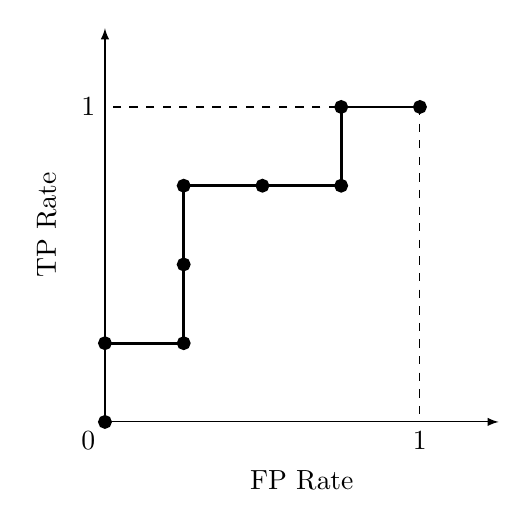
\begin{tikzpicture}
    \coordinate (P0) at (0,0);
    \draw[-latex] (0,0) -- (5,0);
    \draw (2.5,-0.5) node[below] {FP Rate};
    \draw[-latex] (0,0) -- (0,5);
    \draw (-0.5,2.5) node[rotate=90,above] {TP Rate};
    \draw (P0) node [below left]{0};
    \draw[line width=1pt] plot[mark=*] coordinates {(0,0) (0,1) (1,1) (1,2) (1,3) (2,3) (3,3) (3,4) (4,4)};
    \draw[dashed] (4,4) -- (0,4) node[left] {1};
    \draw[dashed] (4,4) -- (4,0) node[below] {1};
  \end{tikzpicture}
  \caption{分类器1 ROC 曲线}
  \label{fig:roc1}
  \end{minipage}
  \begin{minipage}[t]{0.48\textwidth}
  \centering
  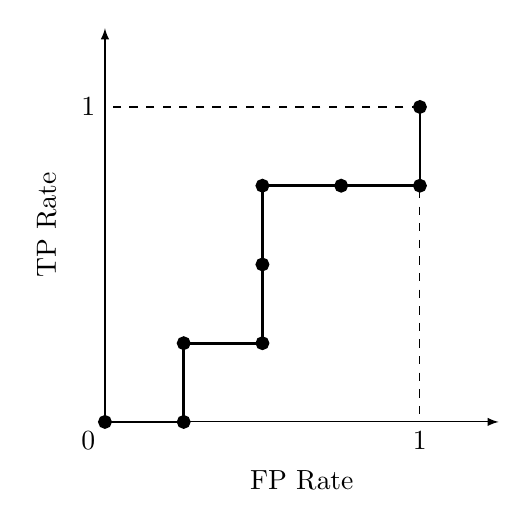
\begin{tikzpicture}
    \coordinate (P0) at (0,0);
    \draw[-latex] (0,0) -- (5,0);
    \draw (2.5,-0.5) node[below] {FP Rate};
    \draw[-latex] (0,0) -- (0,5);
    \draw (-0.5,2.5) node[rotate=90,above] {TP Rate};
    \draw (P0) node [below left]{0};
    \draw[line width=1pt] plot[mark=*] coordinates {(0,0) (1,0) (1,1) (2,1) (2,2) (2,3) (3,3) (4,3) (4,4)};
    \draw[dashed] (4,4) -- (0,4) node[left] {1};
    \draw[dashed] (4,4) -- (4,0) node[below] {1};
  \end{tikzpicture}
  \caption{分类器2 ROC 曲线}
  \label{fig:roc2}
  \end{minipage}
\end{figure}

由图 \ref{fig:roc1} 和图 \ref{fig:roc2} 可得两个分类器的 AUC 分别为
\begin{equation}
  \begin{aligned}
    \mathrm{AUC}_1&=1-5\times\frac{1}{4}\times\frac{1}{4}=\frac{11}{16}\\
    \mathrm{AUC}_2&=7\times\frac{1}{4}\times\frac{1}{4}=\frac{7}{16}\\
  \end{aligned}
\end{equation}

由 $\theta_{1}=0.33$ 和 $\theta_{2}=0.1$ 可知分类器1和分类器2的工作点分别为 (2/4, 3/4) 和 (1, 3/4), 两个工作点的真阳性率相等, 但是分类器1的假阳性率更小, 故在选定工作点处分类器1更好.

越靠近 ROC 曲线左上角的工作点越好, 故对分类器1来说, 工作点 (1/4, 3/4) 最好, 相应的阈值为 $\theta_{1}=0.4$; 对分类器2来说, 工作点 (2/4, 3/4) 最好, 相应的阈值为 $\theta_{2}=0.22$.

\chapter{概率密度函数估计}

统计量:样本的分布信息,如均值,方差等

参数空间:未知参数向量 $\theta$ 全部可能取值的集合 $\Theta$

点估计:构造估计量 $d\left(x_1,\dots ,x_N \right)$ 作为 $\theta$ 的估计

区间估计:构造置信区间 $\left(d_1,d_2 \right)$ 作为 $\theta$ 可能取值范围的估计

\section{极大似然估计 (MLE, Maximum Likelihood Estimate) }

假设:

1. 概率分布函数形式已知

2. 样本独立同分布采样得到

似然函数:
\begin{equation}
\begin{aligned}
  l(\theta)
  &=p(X|\theta)\\
  &=p(x_1,\dots ,x_N|\theta)\\
  &=\prod_kp(x_k|\theta)
\end{aligned}
\end{equation}

对数似然函数:
\begin{equation}
\begin{aligned}
  H(\theta)
  &=\ln l(\theta)\\
  &=\sum_k\ln p(x_k|\theta)
\end{aligned}
\end{equation}

极大似然估计:
\begin{equation}
\begin{aligned}
  \theta 
  &=\mathrm{argmax}_{\theta\in\Theta} l(\theta)\\
  &=\mathrm{argmax}_{\theta\in\Theta} H(\theta)
\end{aligned}
\end{equation}

正态分布:待估计参数为 $\theta=[\mu,\sigma^2]$, 数据点 
\begin{equation}
X=\{ x_1,\dots,x_N\}
\end{equation}

估计量为 $\hat{\theta}=[\hat{\mu},\hat{\sigma}^2]$

概率密度函数为
\begin{equation}
p(x_k|\theta)=\frac{1}{\sqrt{2\pi}\sigma}\exp \left[-\frac{(x_k-\mu)^2}{2\sigma^2} \right]
\end{equation}

取对数得
\begin{equation}
\ln p(x_k|\theta)=-\frac{1}{2}\ln \left(2\pi \theta_2 \right)-\frac{\left(x_k-\theta_1 \right)^2}{2\theta_2}
\end{equation}

对 $\theta$ 求梯度有
\begin{equation}
\nabla_{\theta}\ln p(x_k|\theta)
=\begin{bmatrix}
  \dfrac{x_k-\theta_1}{\theta_2}\\ 
  -\dfrac{1}{2\theta_2}+\dfrac{\left(x_k-\theta_1 \right)^2}{2\theta_{2}^{2}}\\
\end{bmatrix}
\end{equation}

又
\begin{equation}
\sum_{k=1}^N{\nabla_{\theta}\ln p(x_k|\theta)}=0
\end{equation}

因此,估计量为
\begin{equation}
\begin{aligned}
  \hat{\mu}&=\frac{1}{N}\sum_{k=1}^N{x_k} \\
  \hat{\sigma}^2&=\frac{1}{N}\sum_{k=1}^N{\left(x_k-\hat{\mu} \right)^2}
\end{aligned}
\end{equation}

多元正态分布:
\begin{equation}
\begin{aligned}
  \hat{\mu}&=\frac{1}{N}\sum_{k=1}^N{x_k}\\
  \hat{\Sigma}&=\frac{1}{N}\sum_{k=1}^N{\left(x_k-\hat{\mu} \right)\left(x_k-\hat{\mu} \right)^{\top}}
\end{aligned}
\end{equation}

无偏估计:
\begin{equation}
\mathbb{E} \left[\hat{\mu} \right] =\mu
\end{equation}
\begin{equation}
\mathbb{E} \left[\frac{N}{N-1}\hat{\Sigma}\right] =\Sigma
\end{equation}

渐进无偏估计:
\begin{equation}
\lim_{n\rightarrow \infty} \mathbb{E} \left[\hat{\Sigma} \right] =\Sigma
\end{equation}

可识别性:对 $\theta \ne \theta '$, 
\begin{equation}
\exists~x\Rightarrow p(X|\theta)\ne p\left(x|\theta ' \right)
\end{equation}

离散随机变量的混合密度函数往往不可识别,连续的则一般可以识别

\section{贝叶斯估计}

假设:参数 $\theta$ 是随机变量,且已知其先验分布 $p(\theta)$

贝叶斯估计:后验概率
\begin{equation}
p\left(\theta |X \right)=p(X|\theta)p(\theta)/p(x)
\end{equation}

贝叶斯学习:
\begin{equation}
\begin{aligned}
  p\left(x|X \right)
  &=\int{p\left(x,\theta |X \right)\mathrm{d}\theta}\\
  &=\int{p(X|\theta)p\left(\theta |X \right)\mathrm{d}\theta}
\end{aligned}
\end{equation}

贝叶斯学习性质:
\begin{equation}
\lim_{N\rightarrow \infty} p\left(x|X^N \right)=p\left(x|\hat{\theta}=\theta \right)=p(x)
\end{equation}

正态分布:
\begin{equation}
p(X|\mu)\sim \mathcal{N} \left(\mu ,\sigma^2 \right)
\end{equation}
\begin{equation}
p(\mu)\sim \mathcal{N} \left(\mu_o,\sigma_{0}^{2} \right)
\end{equation}

其中 $\sigma^2$ 已知,则有
\begin{equation}
\begin{aligned}
  p(\mu|X)
  &=\frac{p(X|\mu)p(\mu)}{p(x)}\\
  &=\alpha \prod_kp\left(x_k|\mu \right)p(\mu)\\
  &=\alpha '\cdot \exp \left\{ -\frac{1}{2}\left[\sum_{k=1}^N{\frac{\left(\mu -x_k \right)^2}{\sigma^2}}+\frac{\left(\mu -\mu_0 \right)^2}{\sigma_{0}^{2}} \right] \right\} \\
  &:=\frac{1}{\sqrt{2\pi}\sigma_N}\exp \left[-\frac{\left(\mu -\mu_N \right)^2}{2\sigma_{N}^{2}} \right]
\end{aligned}
\end{equation}

其中
\begin{equation}
\sigma_{N}^{2}=\frac{\sigma_{0}^{2}\sigma^2}{N\sigma_{0}^{2}+\sigma^2}
\end{equation}
\begin{equation}
\mu_N=\frac{N\sigma_{0}^{2}}{N\sigma_{0}^{2}+\sigma^2}m_N+\frac{\sigma^2}{N\sigma_{0}^{2}+\sigma^2}\mu_0
\end{equation}

其中
\begin{equation}
m_N=\frac{1}{N}\sum_{k=1}^N{x_k}
\end{equation}

因此
\begin{equation}
\begin{aligned}
  p\left(x|X \right)
  &=\int{p(X|\mu)p(\mu|X)\mathrm{d}\mu}\\
  &\sim \mathcal{N} \left(\mu_N,\sigma^2+\sigma_{N}^{2} \right)
\end{aligned}
\end{equation}

参数变化:
\begin{equation}
\sigma_0=0\Rightarrow \mu_N=\mu_0
\end{equation}
\begin{equation}
N\uparrow \Rightarrow \mu_N\rightarrow m_N,~\sigma_{N}^{2}\rightarrow 0
\end{equation}

最大似然估计与贝叶斯估计对比:

1. 训练样本无穷多时,最大似然估计与贝叶斯估计结果相同

2. 贝叶斯估计使用先验概率利用了更多信息,若信息可靠则贝叶斯估计更准确,但有时先验概率很难设计,无信息先验

3. 最大似然估计计算简单,贝叶斯通常计算复杂的积分

4. 最大似然估计易于理解,给出的是参数的最佳估计结果

\section{非参数估计}

假设:

1. 概率分布函数形式未知

2. 样本独立同分布

直方图估计:
\begin{equation}
\hat{p}_N(x)
=\frac{k_N}{NV_N}
\rightarrow p(x)
\end{equation}

估计收敛条件:
\begin{equation}
V_N\rightarrow 0,~k_N\rightarrow \infty ,~k_N/N\rightarrow 0
\end{equation}

\section{Parzen 窗估计 (Kernel Density Estimation) }

思想:固定小舱体积,滑动小舱估计每个点的概率密度

区域:$R_N$ 是 $d$ 维超立方体,棱长 $h_N$,体积 $V_N=h_{N}^{d}$

窗函数条件:$\displaystyle\phi \left(u \right)\geqslant 0,~\int{\phi \left(u \right)\mathrm{d}u}=1$

1. 方窗:
  \begin{equation}
  \phi \left(u \right)=
  \begin{cases}
    1, &\mathrm{if}~\left\| u \right\|_{\infty}\leqslant 1/2\\
    0, &\mathrm{otherwise}
  \end{cases}
  \end{equation}
2. 正态窗:
  \begin{equation}
  \phi \left(u \right)=\frac{1}{\sqrt{2\pi}}\exp \left(-\frac{1}{2}u^2 \right),~u\in\mathbb{R}
  \end{equation}
3. 指数窗:
  \begin{equation}
  \phi \left(u \right)=\frac{1}{2}\exp \left(-|u| \right),~u\in\mathbb{R}
  \end{equation}

落入以 $x$ 为中心的区域的样本数:
\begin{equation}
k_N=\sum_{i=1}^N{\phi \left(\frac{x-x_i}{h_N} \right)}
\end{equation}

概率密度函数估计:
\begin{equation}
\hat{p}_N(x)=\frac{1}{N}\sum_{i=1}^N{\frac{1}{V_N}\phi \left(\frac{x-x_i}{h_N} \right)}
\end{equation}

窗宽选取:$h_N=h_1/\sqrt{N}$,其中 $h_1$ 可调且一般存在最优值

估计量性质:一维正态窗
\begin{equation}
\begin{aligned}
  \bar{p}_N
  &=\mathbb{E} \left[\hat{p}_N(x)\right] \\
  &\sim \mathcal{N} \left(\mu ,\sigma^2+h_{N}^{2} \right)
\end{aligned}
\end{equation}

\section{\texorpdfstring{$k_N$}{kN} 近邻估计}

思想:固定小舱内数据点个数,滑动可变大小的小舱对每个采样点 (而不是数据点) 进行概率密度估计

数据点个数:$k_N=k_1\sqrt{N}$,其中 $k_1$ 可调且一般存在最优值

\section{估计准确性、维数问题与过拟合}

估计准确性:

1. 贝叶斯误差:不同的类条件概率分布函数之间的相互重叠

2. 模型误差:选择了错误的概率密度函数模型

3. 估计误差:采用有限样本进行估计所带来的误差

维数问题:维数为 $d$,需要样本 $100^d$ →维数灾难

过拟合避免方法:

1. 贝叶斯方法

2. 增加样本数

3. 正则化

4. 减少模型参数

\section{习题}

1. Let $x$ have an exponential density
\begin{equation}
  p(x|\theta)=
  \left\{
    \begin{array}{ll}
      \theta e^{-\theta x}, & x \gs 0 \\
      0,                    & \text {otherwise.}
    \end{array}
  \right.
\end{equation}

1.1 Plot $p(x|\theta)$ versus $x$ for $\theta = 1$. Plot $p(x|\theta)$ versus $\theta$, ($0 \ls \theta \ls 5$) for $x = 2$.

解: 分别如图 \ref{fig:epdf1} 和图 \ref{fig:epdf2} 所示.

\begin{figure}[htbp]
  \centering
  \begin{minipage}[t]{0.48\textwidth}
  \centering
  \includegraphics[width=7cm]{epdf-1.pdf}
  \caption{$p(x|\theta)$ 关于 $x$ 曲线}
  \label{fig:epdf1}
  \end{minipage}
  \begin{minipage}[t]{0.48\textwidth}
  \centering
  \includegraphics[width=7cm]{epdf-2.pdf}
  \caption{$p(x|\theta)$ 关于 $\theta$ 曲线}
  \label{fig:epdf2}
  \end{minipage}
\end{figure}

1.2 Suppose that $n$ samples ${x_1, \cdots, x_n}$ are drawn independently according to $p(x|\theta)$.
Calculate the maximum likelihood estimate for $\theta$.

解: $\theta$ 的最大似然估计应该是下面方程的解
\begin{equation}
  \nabla_\theta H(\theta)=\sum_{k=1}^n\nabla_\theta\ln p(x_k|\theta)=0
\end{equation}

由指数分布可知
\begin{equation}
  \ln p(x_k|\theta)=\ln\theta-\theta x_k,\quad\forall~k=1,2,\cdots,n
\end{equation}

其梯度为
\begin{equation}
  \nabla_\theta\ln p(x_k|\theta)=\frac{1}{\theta}-x_k,\quad\forall~k=1,2,\cdots,n
\end{equation}

因此 $\theta$ 的最大似然估计满足
\begin{equation}
  \sum_{k=1}^n\left(\frac{1}{\hat{\theta}}-x_k\right)=0
\end{equation}

故 $\theta$ 的最大似然估计为
\begin{equation}
  \hat{\theta}=\frac{1}{\displaystyle\frac{1}{n}\sum_{k=1}^nx_k}
\end{equation}

2. The purpose of this problem is to derive the Bayesian classifier for the $d$-dimensional multivariate Bernoulli case. Let $x$ be a $d$-dimensional binary (0 or 1) vector with a multivariate Bernoulli distribution.
\begin{equation}
  p(\bm{x}|\bm{\theta})
  =\prod_{i=1}^{d} \theta_{i}^{x_{i}}\left(1-\theta_{i}\right)^{1-x_{i}},
\end{equation}
where $\bm{\theta}=\left(\theta_{1}, \cdots, \theta_{d}\right)^{T}$ is an unknown parameter vector, $\theta_i$ being the probablility that $x_i=1$. Let $\mathcal{D}$ be a set of $n$ samples $\bm{x}_1, \cdots, \bm{x}_n$ independently drawn according to $p(\bm{x}|\bm{\theta})$. Denote $P\left(\bm{x}_{1}, \cdots, \bm{x}_{n}|\bm{\theta}\right)$ as $P(\mathcal{D}|\bm{\theta})$.

2.1 Calculate the maximum likelihood estimate for $\bm{\theta}$.

解: $\bm{\theta}$ 的最大似然估计应该是下面方程的解
\begin{equation}
  \nabla_{\bm{\theta}} H(\bm{\theta})=\sum_{k=1}^n\nabla_{\bm{\theta}}\ln p(\bm{x}_k|\bm{\theta})=\bm{0}
\end{equation}

由分布函数可知
\begin{equation}
  \ln p(\bm{x}_k|\bm{\theta})=\sum_{i=1}^d\big[x_{k,i}\ln\theta_i+(1-x_{k,i})\ln(1-\theta_i)\big],\quad\forall~k=1,2,\cdots,n
\end{equation}

其对 $\theta_i$ 的梯度为
\begin{equation}
  \nabla_{\theta_i}\ln p(\bm{x}_k|\bm{\theta})=\frac{x_{k,i}}{\theta_i}-\frac{1-x_{k,i}}{1-\theta_i},\quad\forall~k=1,2,\cdots,n,~\forall~i=1,2,\cdots,d
\end{equation}

因此
\begin{equation}
  \sum_{k=1}^n\left(\frac{x_{k,i}}{\theta_i}-\frac{1-x_{k,i}}{1-\theta_i}\right)=0,\quad\forall~i=1,2,\cdots,d
\end{equation}

故 $\theta_i$ 的最大似然估计满足
\begin{equation}
  (1-\hat{\theta}_i)\sum_{k=1}^nx_{k,i}=\hat{\theta}_i\sum_{k=1}^n(1-x_{k,i})=\hat{\theta}_i\left(n-\sum_{k=1}^nx_{k,i}\right),\quad\forall~i=1,2,\cdots,d
\end{equation}

化简得
\begin{equation}
  \hat{\theta}_i=\frac{1}{n}\sum_{k=1}^nx_{k,i},\quad\forall~i=1,2,\cdots,d
\end{equation}

写成向量形式为
\begin{equation}
  \hat{\bm{\theta}}=\frac{1}{n}\sum_{k=1}^n\vx_k
\end{equation}

2.2 Assuming a uniform a priori distribution for $\bm{\theta}$, $0 \ls {\theta}_i \ls 1$, and using the identity
\begin{equation}
  \int_{0}^{1} \theta^{m}(1-\theta)^{n} \mathrm{d}\theta=\frac{m ! n !}{(m+n+1) !},
\end{equation}
calculate the probablility $p(\bm{\theta}|\mathcal{D})$.

解: 令 $\bm{s}$ 表示 $n$ 个样本的和, 即
\begin{equation}
  \bm{s}=\sum_{k=1}^n\vx_k
\end{equation}

则 $P(\mathcal{D}|\bm{\theta})$ 可以计算为
\begin{equation}
  \begin{aligned}
    P(\mathcal{D}|\bm{\theta})
    &=\prod_{k=1}^np(\vx_k|\vtheta)\\
    &=\prod_{k=1}^n\prod_{i=1}^d \theta_{i}^{x_{k,i}}\left(1-\theta_{i}\right)^{1-x_{k,i}}\\
    &=\prod_{i=1}^d\theta_{i}^{s_{i}}\left(1-\theta_{i}\right)^{n-s_{i}}\\
  \end{aligned}
\end{equation}

所以 $p(\mathcal{D})$ 为
\begin{equation}
  \begin{aligned}
    p(\mathcal{D})
    &=\int_{[0,1]^d} P(\mathcal{D}|\bm{\theta})p(\vtheta)\mathrm{d}\vtheta\\
    &=\int_0^1\int_0^1\cdots\int_0^1 \prod_{i=1}^d\theta_{i}^{s_{i}}\left(1-\theta_{i}\right)^{n-s_{i}}\mathrm{d}\theta_1\mathrm{d}\theta_2\cdots\mathrm{d}\theta_d\\
    &=\prod_{i=1}^d\frac{s_i!(n-s_i)!}{(n+1)!}\\
  \end{aligned}
\end{equation}

所以由 Bayes 公式可得概率 $p(\bm{\theta}|\mathcal{D})$ 为
\begin{equation}
  \begin{aligned}
    p(\bm{\theta}|\mathcal{D})
    &=\frac{p(\vtheta,\mathcal{D})}{p(\mathcal{D})}\\
    &=\frac{P(\mathcal{D}|\bm{\theta})p(\vtheta)}{p(\mathcal{D})}\\
    &=\prod_{i=1}^d\frac{(n+1)!}{s_i!(n-s_i)!}\theta_{i}^{s_{i}}\left(1-\theta_{i}\right)^{n-s_{i}}\\
  \end{aligned}
\end{equation}

2.3 Integrate the product $p(\bm{x}|\bm{\theta}) p(\bm{\theta}|\mathcal{D})$ over $\bm{\theta}$ to obtain the desired probability $p(\bm{x}|\mathcal{D})$.

解: 注意到 $x_i\in\{0,1\}$ 则有
\begin{equation}
  \begin{aligned}
    p(\bm{x}|\mathcal{D})
    &=\int_{[0,1]^d} p(\bm{x}|\bm{\theta}) p(\bm{\theta}|\mathcal{D})\mathrm{d}\vtheta\\
    &=\int_{[0,1]^d} \prod_{i=1}^{d} \theta_{i}^{x_{i}}(1-\theta_{i})^{1-x_{i}} \prod_{i=1}^d\frac{(n+1)!}{s_i!(n-s_i)!}\theta_{i}^{s_{i}}(1-\theta_{i})^{n-s_{i}}\mathrm{d}\vtheta\\
    &=\int_0^1\int_0^1\cdots\int_0^1 \prod_{i=1}^{d}\frac{(n+1)!}{s_i!(n-s_i)!}\theta_{i}^{s_{i}+x_{i}}(1-\theta_{i})^{n+1-s_{i}-x_i}\mathrm{d}\theta_1\mathrm{d}\theta_2\cdots\mathrm{d}\theta_d\\
    &=\prod_{i=1}^{d}\frac{(n+1)!}{s_i!(n-s_i)!}\frac{(s_i+x_i)!(n+1-s_i-x_i)!}{(n+2)!}\\
    &=\prod_{i=1}^{d}\frac{1}{n+2}\frac{(s_i+x_i)!}{s_i!}\frac{(n+1-s_i-x_i)!}{(n-s_i)!}\\
    &=\prod_{i=1}^{d}\frac{1}{n+2}(s_i+x_i)^{x_i}(n+1-s_i-x_i)^{1-x_i},\quad x_i\in\{0,1\}\\
    &=\prod_{i=1}^{d}\frac{1}{n+2}(s_i+1)^{x_i}(n+1-s_i)^{1-x_i},\quad x_i\in\{0,1\}\\
    &=\prod_{i=1}^{d}\left(\frac{s_i+1}{n+2}\right)^{x_i}\left(1-\frac{s_i+1}{n+2}\right)^{1-x_i}\\
  \end{aligned}
\end{equation}

2.4 If we think of obtaining $p(\bm{x}|\mathcal{D})$ by substituting an estimate $\hat{\bm{\theta}}$ for $\bm{\theta}$ in $p(\bm{x}|\bm{\theta})$,
what is the effective Bayesian estimate for $\bm{\theta}$?

解: 已知
\begin{equation}
  p(\bm{x}|\bm{\theta})
  =\prod_{i=1}^{d} \theta_{i}^{x_{i}}\left(1-\theta_{i}\right)^{1-x_{i}}
\end{equation}

且由上题有
\begin{equation}
  p(\bm{x}|\mathcal{D})=\prod_{i=1}^{d}\left(\frac{s_i+1}{n+2}\right)^{x_i}\left(1-\frac{s_i+1}{n+2}\right)^{1-x_i}
\end{equation}

根据以上两式, 不难看出参数 $\vtheta$ 的 Bayes 估计为
\begin{equation}
  \hat{\vtheta}_B=\frac{\vs+1}{n+2}=\frac{1}{n+2}\left(\sum_{k=1}^nx_k+1\right)
\end{equation}

2.5 When do maximum likelihood estimation and Bayesian estimation methods differ. (Describe in your own words, not limited to the above examples.)

解: 当训练样本数无穷多的时候, 最大似然估计与 Bayes 估计的结果是一样的, 否则, 他们的结果是不同的.

3. Prove the invariance property of maximum likelihood estimators, i.e., that if $\hat{\theta}$ is the maximum likelihood estimate of $\theta$, then for any differentiable function $\tau(\cdot)$, the maximum likelihood estimate of $\tau(\theta)$ is $\tau(\hat{\theta})$.

证明: 对 $\tau(\theta)$, 文献 \cite{2021george} 基于似然函数 $L(\theta|x)$ 定义导出似然函数 (induced likelihood function) $L^*$ 为
\begin{equation}
  L^*(\eta|x)=\sup_{\{\theta:\tau(\theta)=\eta\}}L(\theta|x)
\end{equation}

令 $\hat{\eta}$ 表示使得导出似然函数取到最大值的变量, 即
\begin{equation}
  \hat{\eta}=\argmax_\eta L^*(\eta|x)
\end{equation}

所以由导出似然函数的定义和最大似然估计的定义可得
\begin{equation}
  \begin{aligned}
    L^*(\hat{\eta}|x)
    &=\sup_\eta\sup_{\{\theta:\tau(\theta)=\eta\}}L(\theta|x)\\
    &=\sup_\theta L(\theta|x)\\
    &=L(\hat{\theta}|x)\\
  \end{aligned}
\end{equation}

又由 $\hat{\theta}$ 是 $\theta$ 的最大似然估计可得
\begin{equation}
  \begin{aligned}
    L(\hat{\theta}|x)
    &=\sup_{\{\theta:\tau(\theta)=\tau(\hat{\theta})\}}L(\theta|x)\\
    &=L^*[\tau(\hat{\theta})|x]
  \end{aligned}
\end{equation}

则
\begin{equation}
  L^*(\hat{\eta}|x)=L^*[\tau(\hat{\theta})|x]
\end{equation}

因此 $\tau(\hat{\theta})$ 是 $\tau(\theta)$ 的最大似然估计.

4. Consider a normal $p(x)\sim N(\mu,\sigma^2)$ and Parzen-window function ${\varphi(x) \sim N(0,1)}$. Show that the Parzen-window estimate
\begin{equation}
  p_{n}(x)=\frac{1}{nh_n} \sum_{i=1}^{n} \varphi\left(\frac{x-x_{i}}{h_{n}}\right)
\end{equation}
has the following properties for small $h_{n}$:

4.1 $\bar{p}_n(x)\sim N(\mu,\sigma^2+h_n^2)$.

解: 令
\begin{equation}
  \theta^2\triangleq\frac{1}{\dfrac{1}{h_n^2}+\dfrac{1}{\sigma^2}}=\frac{h_n^2\sigma^2}{h_n^2+\sigma^2}
\end{equation}
且
\begin{equation}
  \alpha\triangleq\theta^2\left(\frac{x}{h_n^2}+\frac{\mu}{\sigma^2}\right)
\end{equation}

则期望值为
\begin{equation}
  \begin{aligned}
    \bar{p}_{n}(x)
    &=\mathbb{E}[p_n(x)]\\
    &=\frac{1}{nh_n}\sum_{i=1}^n\mathbb{E}\left[\varphi\left(\frac{x-x_{i}}{h_{n}}\right)\right]\\
    &=\frac{1}{h_n}\int_{-\infty}^\infty\varphi\left(\frac{x-v}{h_{n}}\right)p(v)\mathrm{d}v\\
    &=\frac{1}{h_n}\int_{-\infty}^\infty\frac{1}{\sqrt{2\pi}}\exp\left[-\frac{1}{2}\left(\frac{x-v}{h_n}\right)^2\right]\frac{1}{\sqrt{2\pi}\sigma}\exp\left[-\frac{1}{2}\left(\frac{v-\mu}{\sigma}\right)^2\right]\mathrm{d}v\\
    &=\frac{1}{2\pi h_n\sigma}\exp\left[-\frac{1}{2}\left(\frac{x^2}{h_n^2}+\frac{\mu^2}{\sigma^2}\right)\right]\int_{-\infty}^\infty\exp\left\{-\frac{1}{2}\left[v^2\left(\frac{1}{h_n^2}+\frac{1}{\sigma^2}\right)-2v\left(\frac{x}{h_n^2}+\frac{\mu}{\sigma^2}\right)\right]\right\}\mathrm{d}v\\
    &=\frac{1}{2\pi h_n\sigma}\exp\left[-\frac{1}{2}\left(\frac{x^2}{h_n^2}+\frac{\mu^2}{\sigma^2}\right)+\frac{1}{2}\frac{\alpha^2}{\theta^2}\right]\int_{-\infty}^\infty\exp\left[-\frac{1}{2}\left(\frac{v-\alpha}{\theta}\right)^2\right]\mathrm{d}v\\
    &=\frac{\sqrt{2\pi}\theta}{2\pi h_n\sigma}\exp\left[-\frac{1}{2}\left(\frac{x^2}{h_n^2}+\frac{\mu^2}{\sigma^2}-\frac{\alpha^2}{\theta^2}\right)\right]\\
    &=\frac{1}{\sqrt{2\pi}h_n\sigma}\frac{h_n\sigma}{\sqrt{h_n^2+\sigma^2}}\exp\left[-\frac{1}{2}\left(\frac{x^2\sigma^2+h_n^2\mu^2}{h_n^2\sigma^2}-\frac{h_n^2\sigma^2}{h_n^2+\sigma^2}\frac{(x\sigma^2+h_n^2\mu)^2}{(h_n^2\sigma^2)^2}\right)\right]\\
    &=\frac{1}{\sqrt{2\pi}\sqrt{h_n^2+\sigma^2}}\exp\left[-\frac{1}{2}\frac{(x^2\sigma^2+h_n^2\mu^2)(h_n^2+\sigma^2)-(x\sigma^2+h_n^2\mu)^2}{h_n^2\sigma^2(h_n^2+\sigma^2)}\right]\\
    &=\frac{1}{\sqrt{2\pi}\sqrt{h_n^2+\sigma^2}}\exp\left[-\frac{1}{2}\frac{x^2\sigma^2h_n^2+\mu^2h_n^2\sigma^2-2x\mu h_n^2\sigma^2}{h_n^2\sigma^2(h_n^2+\sigma^2)}\right]\\
    &=\frac{1}{\sqrt{2\pi}\sqrt{h_n^2+\sigma^2}}\exp\left[-\frac{1}{2}\left(\frac{x-\mu}{\sqrt{h_n^2+\sigma^2}}\right)^2\right]\\
  \end{aligned}
\end{equation}

因此
\begin{equation}
  \bar{p}_n(x)\sim N(\mu,\sigma^2+h_n^2)
\end{equation}

4.2 $\text{Var}[p_n(x)]\simeq\dfrac{1}{2nh_n\sqrt{\pi}}p(x)$.

解: 由 4.1 可知, 当 $h_n$ 充分小时, 有
\begin{equation}
  \bar{p}_n(x)\sim N(\mu,\sigma^2)
\end{equation}

即有
\begin{equation}
  \frac{1}{h_n}\mathbb{E}\left[\varphi\left(\frac{x-v}{h_{n}}\right)\right]\simeq p(x)
\end{equation}

则当 $h_n$ 充分小时, 利用上述结论以及 $x_1,x_2,\cdots,x_n$ 的独立性可得方差为
\begin{equation}
  \begin{aligned}
    \text{Var}[p_n(x)]
    &=\text{Var}\left[\frac{1}{nh_n}\sum_{i=1}^{n} \varphi\left(\frac{x-x_{i}}{h_{n}}\right)\right]\\
    &=\frac{1}{n^2h_n^2}\sum_{i=1}^{n}\text{Var} \left[\varphi\left(\frac{x-x_{i}}{h_{n}}\right)\right]\\
    &=\frac{1}{nh_n^2}\text{Var} \left[\varphi\left(\frac{x-v}{h_{n}}\right)\right]\\
    &=\frac{1}{nh_n^2}\left\{\mathbb{E}\left[\varphi^2\left(\frac{x-v}{h_{n}}\right)\right]-\mathbb{E}^2\left[\varphi\left(\frac{x-v}{h_{n}}\right)\right]\right\}\\
    &=\frac{1}{nh_n^2}\left\{\frac{1}{\sqrt{2\pi}}\mathbb{E}\left[\varphi\left(\frac{x-v}{h_{n}/\sqrt{2}}\right)\right]-\mathbb{E}^2\left[\varphi\left(\frac{x-v}{h_{n}}\right)\right]\right\}\\
    &=\frac{1}{2nh_n\sqrt{\pi}}\frac{1}{h_n/\sqrt{2}}\mathbb{E}\left[\varphi\left(\frac{x-v}{h_{n}/\sqrt{2}}\right)\right]-\frac{1}{n}\left\{\frac{1}{h_n}\mathbb{E}\left[\varphi\left(\frac{x-v}{h_{n}}\right)\right]\right\}^2\\
    &\simeq\frac{p(x)}{2nh_n\sqrt{\pi}}\Big[1-2\sqrt{\pi}h_np(x)\Big]\\
    &\simeq\frac{p(x)}{2nh_n\sqrt{\pi}}
  \end{aligned}
\end{equation}

4.3 $\displaystyle p(x)-\bar{p}_{n}(x) \simeq \frac{1}{2}\left(\frac{h_{n}}{\sigma}\right)^{2}\left[1-\left(\frac{x-\mu}{\sigma}\right)^{2}\right] p(x)$.

解: 偏差为
\begin{equation}
  \begin{aligned}
    p(x)-\bar{p}_n(x)
    &=p(x)\left[1-\frac{\bar{p}_n(x)}{p(x)}\right]\\
    &=p(x)\left\{1-\frac{\sigma}{\sqrt{\sigma^2+h_n^2}}\exp\left[-\frac{1}{2}\frac{(x-\mu)^2}{\sigma^2+h_n^2}+\frac{1}{2}\frac{(x-\mu)^2}{\sigma^2}\right]\right\}\\
    &=p(x)\left\{1-\frac{1}{\sqrt{1+(h_n/\sigma)^2}}\exp\left[\frac{1}{2}\frac{h_n^2}{\sigma^2}\frac{(x-\mu)^2}{\sigma^2+h_n^2}\right]\right\}\\
  \end{aligned}
\end{equation}

当 $h_n$ 充分小时, 有
\begin{equation}
  \frac{1}{\sqrt{1+(h_n/\sigma)^2}}\simeq 1-\frac{1}{2}\frac{h_n^2}{\sigma^2}
\end{equation}

和
\begin{equation}
  \exp\left[\frac{1}{2}\frac{h_n^2}{\sigma^2}\frac{(x-\mu)^2}{\sigma^2+h_n^2}\right]\simeq 1+\frac{1}{2}\frac{h_n^2}{\sigma^2}\frac{(x-\mu)^2}{\sigma^2+h_n^2}
\end{equation}

所以
\begin{equation}
  \begin{aligned}
    p(x)-\bar{p}_n(x)
    &\simeq p(x)\left[1-\left(1-\frac{1}{2}\frac{h_n^2}{\sigma^2}\right)\left(1+\frac{1}{2}\frac{h_n^2}{\sigma^2}\frac{(x-\mu)^2}{\sigma^2+h_n^2}\right)\right]\\
    &\simeq p(x)\left[1-1+\frac{1}{2}\frac{h_n^2}{\sigma^2}-\frac{1}{2}\frac{h_n^2}{\sigma^2}\frac{(x-\mu)^2}{\sigma^2+h_n^2}\right]\\
    &=\frac{1}{2}\frac{h_n^2}{\sigma^2}p(x)\left[1-\frac{(x-\mu)^2}{\sigma^2+h_n^2}\right]\\
    &\simeq \frac{1}{2}\left(\frac{h_{n}}{\sigma}\right)^{2}\left[1-\left(\frac{x-\mu}{\sigma}\right)^{2}\right] p(x)\\
  \end{aligned}
\end{equation}

5. Consider classifiers based on samples from the distributions
\begin{equation}
  p\left(x|\omega_{1}\right)=
  \left\{
    \begin{array}{ll}
      3 / 2, & \text { for } 0 \ls x \ls 2 / 3 \\
      0,     & \text { otherwise }
    \end{array}
  \right.
\end{equation}
and
\begin{equation}
  p\left(x|\omega_{2}\right)=
  \left\{
    \begin{array}{ll}
      3 / 2, & \text { for } 1 / 3 \ls x \ls 1 \\
      0,     & \text { otherwise. }
    \end{array}
  \right.
\end{equation}

5.1  What is the Bayes decision rule and the Bayes classification error?

解: 假定 $P(\omega_1)=P(\omega_2)$, 则边界点
\begin{equation}
  t\in\left[\frac{1}{3},~\frac{2}{3}\right]
\end{equation}

取定 $t$, 则 Bayes 决策为
\begin{equation}
  \begin{aligned}
    x\in(0,t)&\to x\in\omega_1\\
    x\in(t,1)&\to x\in\omega_2\\
  \end{aligned}
\end{equation}

Bayes 决策错误率为
\begin{equation}
  \begin{aligned}
    P_B(e)
    &=P(\omega_1)\int_{t}^1p(x|\omega_1)\mathrm{d}x+P(\omega_2)\int_{0}^tp(x|\omega_2)\mathrm{d}x\\
    &=\frac{1}{2}\int_{t}^{2/3}\frac{3}{2}\mathrm{d}x+\frac{1}{2}\int_{1/3}^{t}\frac{3}{2}\mathrm{d}x\\
    &=\frac{1}{2}\times\frac{3}{2}\times\frac{1}{3}\\
    &=\frac{1}{4}\\
  \end{aligned}
\end{equation}

5.2 Suppose we randomly select a single point from $\omega_{1}$ and a single point from $\omega_{2}$, and create a nearest-neighbor classifier. Suppose too we select a test point from one of the categories ($\omega_{1}$ for definiteness). Integrate to find the expected error rate $P_{1}(e)$.

解: 设从 $\omega_1$ 中取出的点为 $x_1$, 从 $\omega_2$ 中取出的点为 $x_2$, 则最近邻法的分类边界点为
\begin{equation}
  t=\frac{x_1+x_2}{2}
\end{equation}

$x_1$ 与 $x_2$ 的取值范围构成的区域如图 \ref{fig:sampleRange} 所示, 根据 $x_1$ 与 $x_2$ 之间的大小关系和边界点 $t$ 所处的不同区间可以分成4个子区域, 下面分类讨论.

\begin{figure}
  \centering
  \begin{tikzpicture}
    \coordinate (P0) at (0,0);
    \draw[-latex] (0,0) -- (7,0);
    \draw (7,0) node[below] {$x_1$};
    \draw[-latex] (0,0) -- (0,7);
    \draw (0,7) node[left] {$x_2$};
    \draw (P0) node [below left]{0};
    \draw plot coordinates {(0,2) (4,2) (4,6) (0,6) (0,2)};
    \draw[dashed] (2,2) -- (4,4);
    \draw[dashed] (4,4) -- (2,6);
    \draw[dashed] (0,4) -- (2,2);
    \draw[dashed] (4,2) -- (4,0);
    \draw (0,6) node[left] {1};
    \draw (0,4) node[left] {$\dfrac{2}{3}$};
    \draw (0,2) node[left] {$\dfrac{1}{3}$};
    \draw (2,0) node[below] {$\dfrac{1}{3}$};
    \draw (4,0) node[below] {$\dfrac{2}{3}$};
    \draw (6,0) node[below] {1};
    \draw (3.4,2.6) node {1};
    \draw (2,4) node {2};
    \draw (0.6, 2.6) node {3};
    \draw (3.4,5.4) node {4};
  \end{tikzpicture}
  \caption{从两个类别中取出的采样点构成的区域}
  \label{fig:sampleRange}
\end{figure}

在区域1中, $x_1\gs x_2$, 且 $t\in[1/3,2/3]$, 所以该区域的错误率可以计算为
\begin{equation}
  P_1(e_1)=\frac{1}{8}\left(\frac{1}{2}\int_{0}^t\frac{3}{2}\mathrm{d}x+\frac{1}{2}\int_t^{1}\frac{3}{2}\mathrm{d}x\right)=\frac{3}{32}
\end{equation}

在区域2中, $x_1\ls x_2$, 且 $t\in[1/3,2/3]$, 所以该区域的错误率可以计算为
\begin{equation}
  P_1(e_2)=\frac{5}{8}\left(\frac{1}{2}\int_{t}^{2/3}\frac{3}{2}\mathrm{d}x+\frac{1}{2}\int_{1/3}^{t}\frac{3}{2}\mathrm{d}x\right)=\frac{5}{32}
\end{equation}

在区域3中, $x_1\ls x_2$, 且 $t\in[0,1/3]$, 所以该区域的错误率可以计算为
\begin{equation}
  P_1(e_3)=\frac{9}{4}\int_0^{1/3}\int_{1/3}^{2/3-x_1}\left(\frac{1}{2}\int_t^{2/3}\frac{3}{2}\mathrm{d}x\right)\mathrm{d}x_2~\mathrm{d}x_1=\frac{7}{192}
\end{equation}

在区域4中, $x_1\ls x_2$, 且 $t\in[2/3,1]$, 所以该区域的错误率可以计算为
\begin{equation}
  P_1(e_4)=\frac{9}{4}\int_{1/3}^{2/3}\int_{4/3-x_1}^{1}\left(\frac{1}{2}\int_{1/3}^{t}\frac{3}{2}\mathrm{d}x\right)\mathrm{d}x_2~\mathrm{d}x_1=\frac{7}{192}
\end{equation}

故总错误率为
\begin{equation}
  P_1(e)=\sum_{k=1}^4P_1(e_k)=\frac{3}{32}+\frac{5}{32}+\frac{7}{192}+\frac{7}{192}=\frac{31}{96}\approx0.3329
\end{equation}

5.3 With the limit of the training sample number $n \rightarrow \infty$, compare the expected error $P_{n}(e)$ with the Bayes error.

解: 当 $n\to\infty$ 时, 只有位于区间 [1/3, 2/3] 之内的测试点会被错分, 且错分概率为 0.5, 则错误率为
\begin{equation}
  \begin{aligned}
    P_\infty(e)
    &\triangleq\lim_{n\to\infty}P_n(e)\\
    &=\frac{1}{2}P(\omega_1)P\left(\frac{1}{3}\ls x\ls\frac{2}{3}\bigg|\omega_1\right)+\frac{1}{2}P(\omega_2)P\left(\frac{1}{3}\ls x\ls\frac{2}{3}\bigg|\omega_2\right)\\
    &=\frac{1}{2}\times\frac{1}{2}\times\frac{1}{2}+\frac{1}{2}\times\frac{1}{2}\times\frac{1}{2}\\
    &=\frac{1}{4}\\
  \end{aligned}
\end{equation}

因此 $P_\infty(e)=P_B(e)$, 即误差率相等.

5.4 What are the factors that affect the classification error rate?

解: 在本题中, 影响误差率的因素主要是两类条件概率密度的重合区间长度, 重合区间越长, 则错误率越大.

6. Assume  $p(x) \sim 0.2~\mathcal{N}(-1,1)+0.8~\mathcal{N}(1,1)$.  Draw $n$ samples from $p(x)$, for example, 
\begin{equation}
  n=5,10,50,100,\cdots,1000,\cdots,10000.
\end{equation} 
Use Parzen-window method to estimate $p_n(x)\approx p(x)$. (Hint: use randn() function in matlab to draw samples.)

(a) Try window-function 
\begin{equation}
  K(x)=
  \left\{
    \begin{array}{ll}
      \dfrac{1}{a},&-\dfrac{a}{2}\ls x\ls \dfrac{a}{2} \\
      0, & \text{otherwise.}
    \end{array}
  \right.
\end{equation} 
Estimate $p(x)$ with different window width $a$. Please draw $p_n(x)$ under different $n$ and $a$ and $p(x)$ to show the estimation effect.

解: 取 $n=5,10,50,100,1000,5000$, $a=0.25,0.5,1,2,4,8$, 使用方窗函数进行估计, 结果如图 \ref{fig:sqwin} 所示, 图中红色曲线表示 $p(x)$. 由图可知, 固定 $a$ 时, 随着 $n$ 的增大, 估计效果逐渐变好; 固定 $n$ 时, 随着 $a$ 的增大, 估计效果先变好后变差, 可知存在适当的 $a$ 使得估计效果达到最好.

\begin{figure}[htbp]
  \centering
  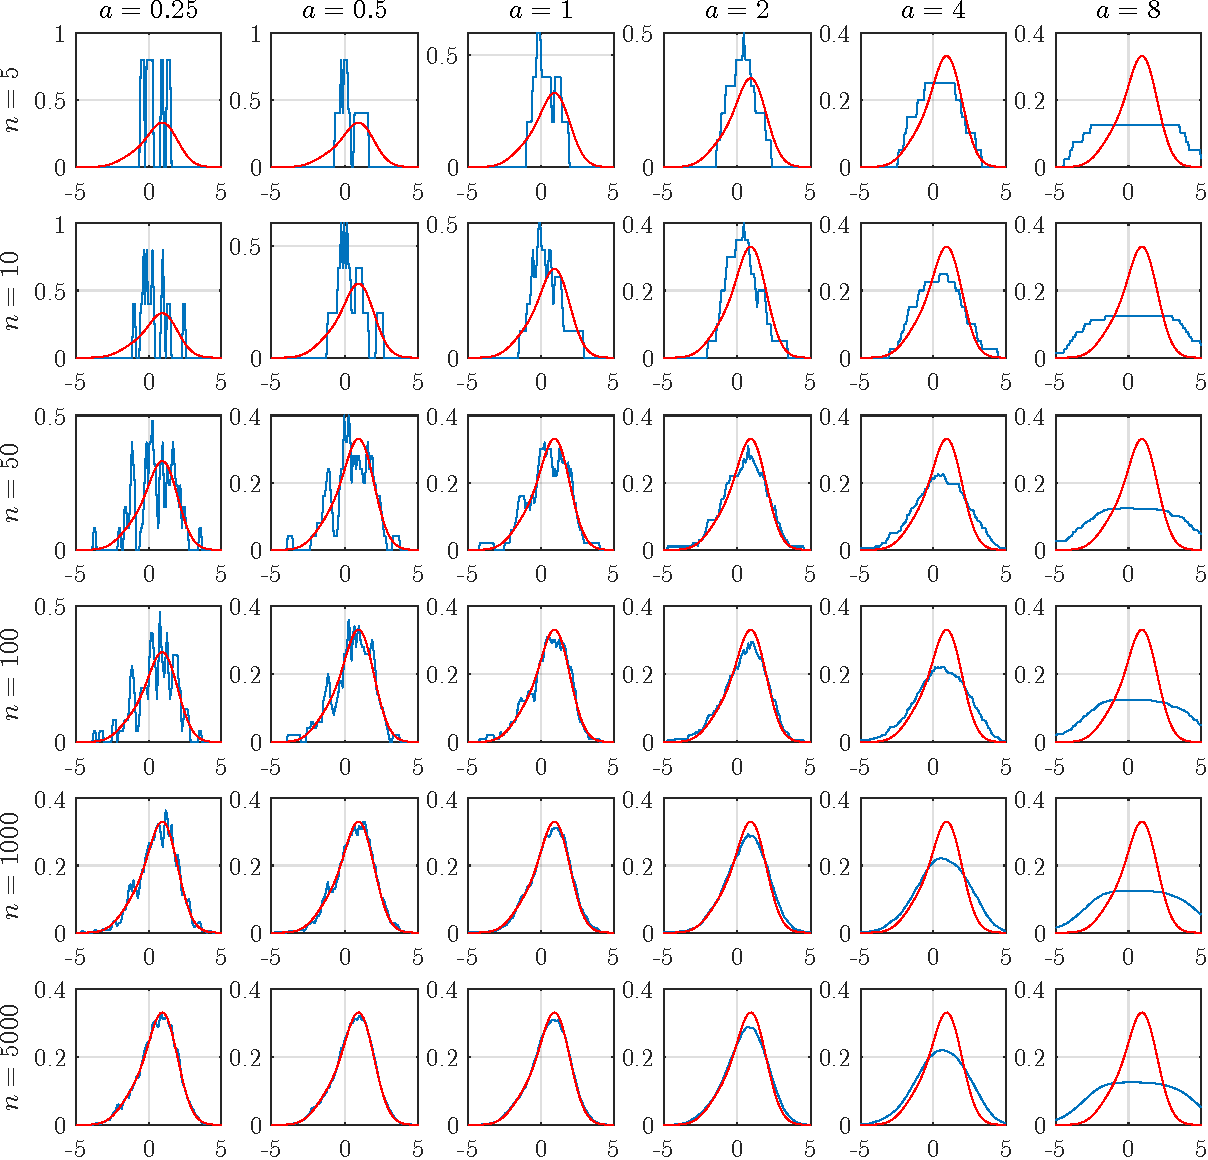
\includegraphics[width=0.9\textwidth]{squareWindow.pdf}
  \caption{方窗估计}
  \label{fig:sqwin}
\end{figure}

(b) Derive how to compute
\begin{equation}
  \epsilon(p_n)=\int\big[p_n(x)-p(x)\big]^2\mathrm{d}x
\end{equation}
numerically.

解: 取积分区间为 [-5, 5], 将区间 $N$ 等分, 记区间长度为 $\Delta \xi$, $\xi_j$ 为第 $j$ 个区间内一点, 当 $N$ 足够大时, 有
\begin{equation}
  \begin{aligned}
    \epsilon(p_n)
    &=\int\big[p_n(x)-p(x)\big]^2\mathrm{d}x\\
    &\simeq\sum_{j=1}^N\big[p_n(\xi_j)-p(\xi_j)\big]^2\Delta \xi\\
    &=\sum_{j=1}^N\left\{\frac{1}{n}\sum_{i=1}^nK(\xi_j-x_i)-\frac{0.2}{\sqrt{2\pi}}\exp\left[-\frac{(\xi_j+1)^2}{2}\right]-\frac{0.8}{\sqrt{2\pi}}\exp\left[-\frac{(\xi_j-1)^2}{2}\right]\right\}^2\Delta \xi\\
  \end{aligned}
\end{equation}

(c) Demonstrate the expectation and variance of $\epsilon(p_n)$ w.r.t different $n$ and $a$.

解: 为了数值计算 $\epsilon(p_n)$ 的期望和方差, 对每一组给定的 $(n,a)$, 进行多次重复试验, 而后对多次试验得到的 $\epsilon(p_n)$ 数组计算均值和方差, 结果分别如表 \ref{tab:squMeanMSE} 和表 \ref{tab:squVarMSE} 所示.

\begin{table}[htbp]
  \centering
  \begin{tabular}{l|cccccc}
  \hline
           & $a=0.25$ & $a=0.5$ & $a=1$  & $a=2$  & $a=4$  & $a=8$  \\ 
  \hline
  $n=5$    & 0.0754   & 0.0344  & 0.0153 & 0.0051 & 0.0038 & 0.0086 \\
  $n=10$   & 0.0377   & 0.0200  & 0.0088 & 0.0035 & 0.0025 & 0.0084 \\
  $n=50$   & 0.0079   & 0.0038  & 0.0017 & 0.0009 & 0.0025 & 0.0083 \\
  $n=100$  & 0.0040   & 0.0016  & 0.0009 & 0.0004 & 0.0019 & 0.0083 \\
  $n=1000$ & 0.0003   & 0.0001  & 0.0001 & 0.0002 & 0.0020 & 0.0083 \\
  $n=5000$ & 0.0001   & 0.0000  & 0.0000 & 0.0002 & 0.0020 & 0.0083 \\ 
  \hline
  \end{tabular}
  \caption{方窗估计均方误差期望}
  \label{tab:squMeanMSE}
\end{table}

\begin{table}[htbp]
  \centering
  \begin{tabular}{l|cccccc}
  \hline
           & $a=0.25$   & $a=0.5$    & $a=1$      & $a=2$      & $a=4$      & $a=8$      \\ \hline
  $n=5$    & 0          & 5.2849e-05 & 5.0611e-05 & 1.1692e-05 & 4.3810e-06 & 1.6058e-07 \\
  $n=10$   & 8.6365e-05 & 5.2020e-05 & 2.4856e-05 & 1.0281e-05 & 5.3322e-07 & 9.2295e-08 \\
  $n=50$   & 5.5701e-06 & 3.1296e-06 & 9.1607e-07 & 5.1668e-07 & 3.5719e-07 & 2.0359e-08 \\
  $n=100$  & 1.4699e-06 & 4.4399e-07 & 1.3575e-07 & 4.8224e-08 & 7.9064e-08 & 5.5102e-09 \\
  $n=1000$ & 6.1293e-09 & 3.7063e-09 & 2.0755e-09 & 5.9962e-09 & 4.8550e-09 & 6.2758e-10 \\
  $n=5000$ & 0          & 4.8334e-41 & 4.8334e-41 & 6.9602e-39 & 0          & 3.1676e-36 \\ \hline
  \end{tabular}
  \caption{方窗估计均方误差方差}
  \label{tab:squVarMSE}
\end{table}

(d) With $n$ given, how to choose optimal $a$ from above the empirical experiences?

解: 由以上经验, 对于给定的 $n$, 可以通过 $\epsilon(p_n)$ 的均值和方差来选取适当的 $a$ 值. 固定 $n$ 时, 随着 $a$ 的增大, 估计效果先变好后变差, 所以 $a$ 在适当的取值下才能最好地逼近真实概率密度函数, 因此可以将 $\epsilon(p_n)$ 的均值与 $a$ 的函数关系绘制出来, 寻找其最小值所在区间, 并在该区间内选择 $\epsilon(p_n)$ 最小方差对应的 $a$.

(e) Substitute $K(x)$ in (a) with Gaussian window. Repeat (a)-(d).

解: 取 $n=5,10,50,100,1000,5000$, $a=0.25,0.5,1,2,4,8$, 使用高斯核函数
\begin{equation}
  K(x)=\frac{1}{\sqrt{2\pi}\sigma}\exp\left[-\frac{x^2}{2\sigma^2}\right]
\end{equation}
进行估计, 其中取 $\sigma=a/\sqrt{n}$, 结果如图 \ref{fig:gauwin} 所示, 图中红色曲线表示 $p(x)$. 对每一组给定的 $(n,a)$, 进行多次重复试验, 而后对多次试验得到的 $\epsilon(p_n)$ 数组计算均值和方差, 结果分别如表 \ref{tab:gauMeanMSE} 和表 \ref{tab:gauVarMSE} 所示.

\begin{figure}[htbp]
  \centering
  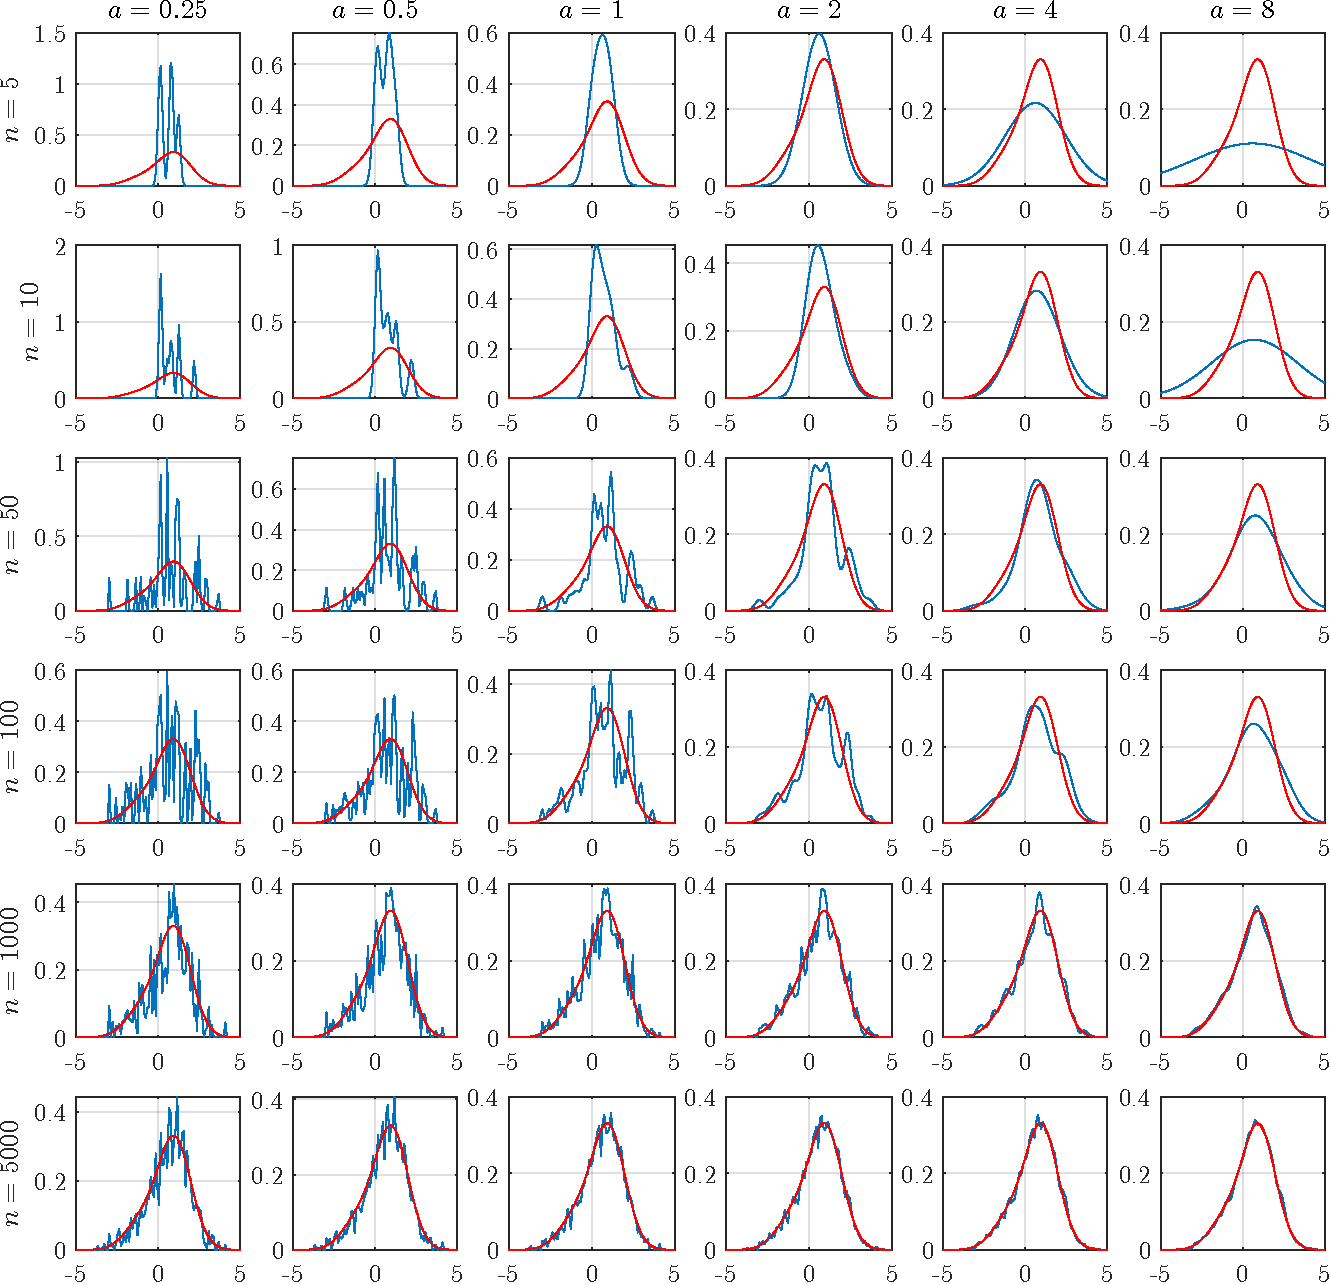
\includegraphics[width=0.9\textwidth]{gaussianWindow.pdf}
  \caption{高斯估计}
  \label{fig:gauwin}
\end{figure}

\begin{table}[htbp]
  \centering
  \begin{tabular}{l|cccccc}
  \hline
           & $a=0.25$ & $a=0.5$ & $a=1$  & $a=2$  & $a=4$  & $a=8$  \\ \hline
  $n=5$    & 0.0440   & 0.0186  & 0.0088 & 0.0055 & 0.0041 & 0.0095 \\
  $n=10$   & 0.0330   & 0.0168  & 0.0062 & 0.0022 & 0.0025 & 0.0065 \\
  $n=50$   & 0.0147   & 0.0077  & 0.0031 & 0.0017 & 0.0007 & 0.0015 \\
  $n=100$  & 0.0110   & 0.0052  & 0.0024 & 0.0011 & 0.0005 & 0.0007 \\
  $n=1000$ & 0.0035   & 0.0019  & 0.0009 & 0.0004 & 0.0002 & 0.0001 \\
  $n=5000$ & 0.0011   & 0.0007  & 0.0003 & 0.0002 & 0.0001 & 0.0000 \\ \hline
  \end{tabular}
  \caption{高斯估计均方误差期望}
  \label{tab:gauMeanMSE}
\end{table}

\begin{table}[htbp]
  \centering
  \begin{tabular}{l|cccccc}
  \hline
           & $a=0.25$   & $a=0.5$    & $a=1$      & $a=2$      & $a=4$      & $a=8$      \\ \hline
  $n=5$    & 8.8794e-05 & 3.5598e-05 & 3.2554e-05 & 5.0078e-05 & 2.1877e-06 & 1.0487e-07 \\
  $n=10$   & 6.2303e-05 & 3.7369e-05 & 6.7287e-06 & 2.0091e-06 & 1.9361e-06 & 1.2545e-07 \\
  $n=50$   & 7.7749e-06 & 9.8888e-06 & 1.4582e-06 & 8.6869e-07 & 1.8728e-07 & 1.7556e-07 \\
  $n=100$  & 9.5059e-06 & 2.0828e-06 & 5.2320e-07 & 3.1134e-07 & 9.8478e-08 & 1.1429e-07 \\
  $n=1000$ & 5.2851e-07 & 9.1313e-08 & 5.3496e-08 & 1.0761e-08 & 5.6957e-09 & 1.6131e-09 \\
  $n=5000$ & 6.6818e-38 & 7.0530e-38 & 1.6240e-38 & 7.4242e-39 & 5.7711e-39 & 5.6068e-39 \\ \hline
  \end{tabular}
  \caption{高斯估计均方误差方差}
  \label{tab:gauVarMSE}
\end{table}

(f) Try different window functions and parameters as many as you can. Which window function/parameter is the best one? Demonstrate it numerically.

解: 取 $n=5,10,50,100,1000,5000$, $a=0.25,0.5,1,2,4,8$, 使用三角形核函数
\begin{equation}
  K(x)=
  \left\{
    \begin{array}{ll}
      \dfrac{1}{a}\left(1-\left\lvert\dfrac{x}{a} \right\rvert\right),&-a\ls x\ls a \\
      0, & \text{otherwise.}
    \end{array}
  \right.
\end{equation}
进行估计, 结果如图 \ref{fig:triwin} 所示, 图中红色曲线表示 $p(x)$. 对每一组给定的 $(n,a)$, 进行多次重复试验, 而后对多次试验得到的 $\epsilon(p_n)$ 数组计算均值和方差, 结果分别如表 \ref{tab:triMeanMSE} 和表 \ref{tab:triVarMSE} 所示.

\begin{figure}[htbp]
  \centering
  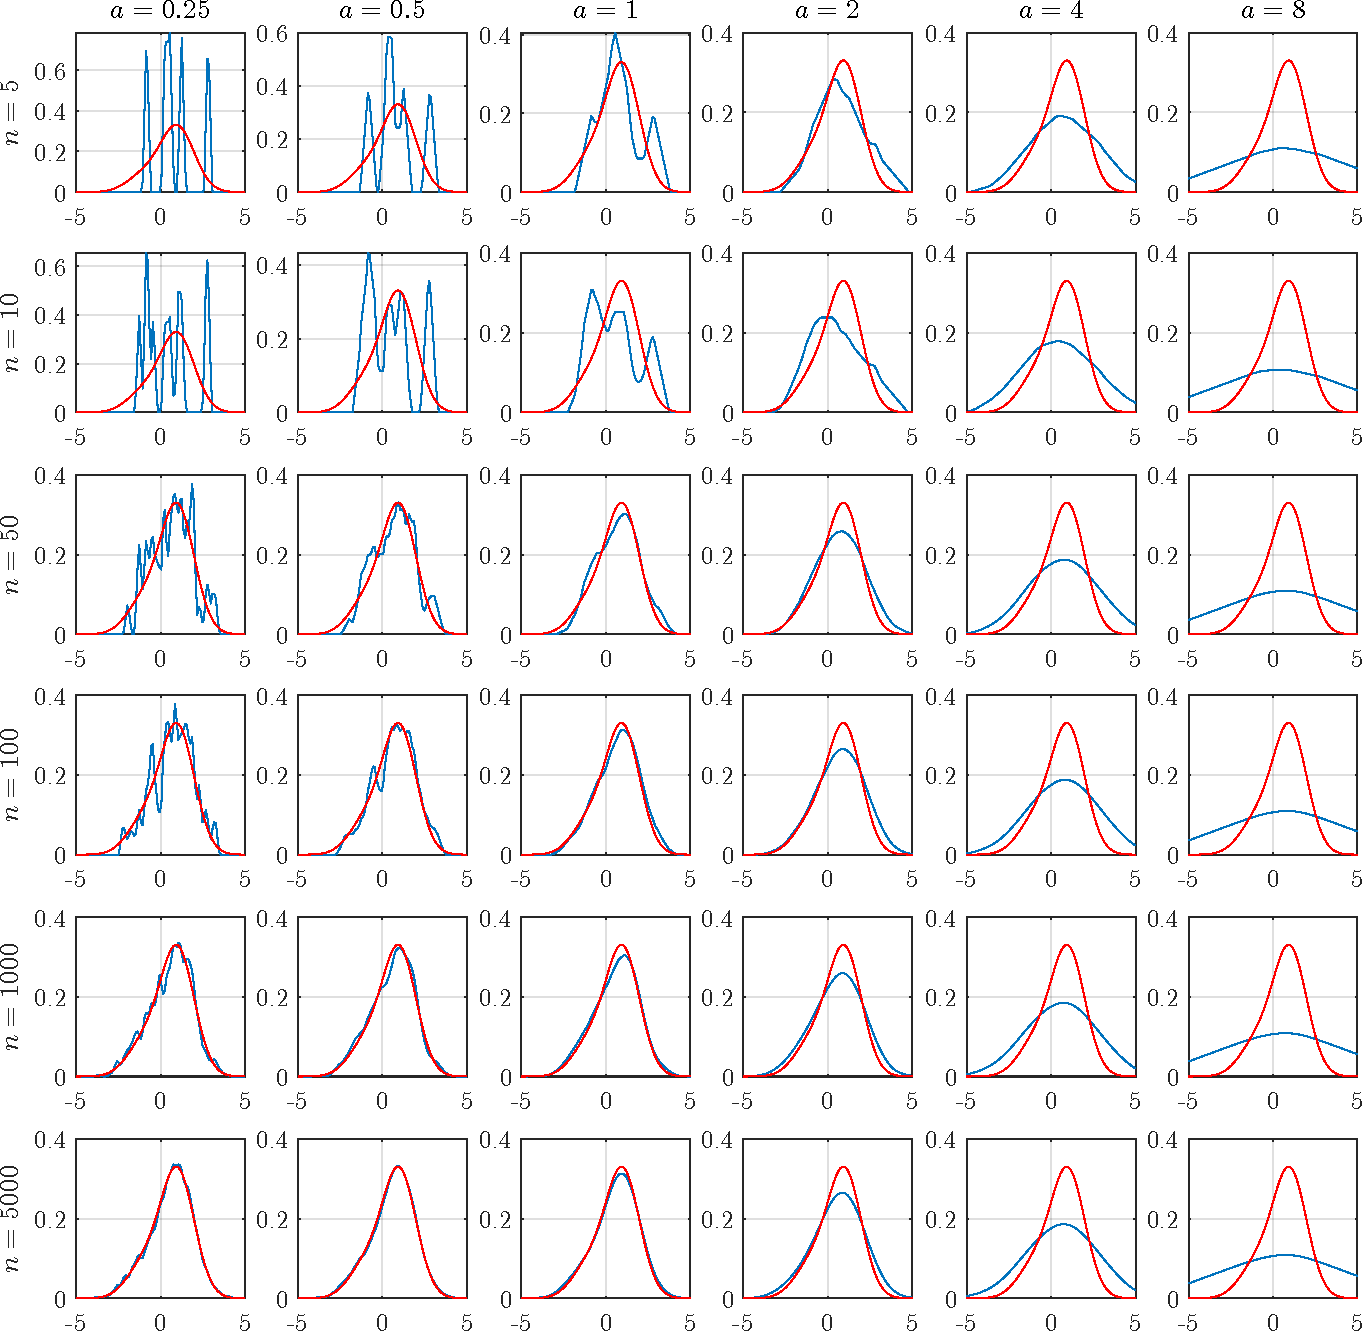
\includegraphics[width=0.9\textwidth]{triangularWindow.pdf}
  \caption{三角形估计}
  \label{fig:triwin}
\end{figure}

\begin{table}[htbp]
  \centering
  \begin{tabular}{l|cccccc}
  \hline
           & $a=0.25$ & $a=0.5$ & $a=1$  & $a=2$  & $a=4$  & $a=8$  \\ \hline
  $n=5$    & 0.0456   & 0.0231  & 0.0085 & 0.0038 & 0.0045 & 0.0092 \\
  $n=10$   & 0.0250   & 0.0113  & 0.0049 & 0.0021 & 0.0038 & 0.0094 \\
  $n=50$   & 0.0050   & 0.0024  & 0.0009 & 0.0011 & 0.0037 & 0.0092 \\
  $n=100$  & 0.0020   & 0.0011  & 0.0005 & 0.0008 & 0.0038 & 0.0092 \\
  $n=1000$ & 0.0002   & 0.0001  & 0.0001 & 0.0006 & 0.0036 & 0.0092 \\
  $n=5000$ & 0.0000   & 0.0000  & 0.0001 & 0.0006 & 0.0036 & 0.0092 \\ \hline
  \end{tabular}
  \caption{三角估计均方误差期望}
  \label{tab:triMeanMSE}
\end{table}

\begin{table}[htbp]
  \centering
  \begin{tabular}{l|cccccc}
  \hline
           & $a=0.25$   & $a=0.5$    & $a=1$      & $a=2$      & $a=4$      & $a=8$      \\ \hline
  $n=5$    & 7.1407e-05 & 1.3686e-04 & 2.7454e-05 & 9.2369e-06 & 1.8634e-06 & 1.6729e-07 \\
  $n=10$   & 4.9860e-05 & 2.2354e-05 & 7.8718e-06 & 4.1982e-06 & 6.1847e-07 & 1.9638e-07 \\
  $n=50$   & 3.1465e-06 & 1.1115e-06 & 2.8525e-07 & 3.0190e-07 & 1.1315e-07 & 1.1064e-08 \\
  $n=100$  & 3.4641e-07 & 1.4459e-07 & 1.6658e-07 & 7.9556e-08 & 7.8658e-08 & 1.0195e-08 \\
  $n=1000$ & 3.8268e-09 & 2.1874e-09 & 1.6549e-09 & 4.0677e-09 & 6.4841e-09 & 8.1923e-10 \\
  $n=5000$ & 1.3256e-39 & 8.1878e-40 & 3.6360e-38 & 1.1693e-37 & 1.0988e-36 & 7.7607e-36 \\ \hline
  \end{tabular}
  \caption{三角估计均方误差方差}
  \label{tab:triVarMSE}
\end{table}

取 $n=5,10,50,100,1000,5000$, $a=0.25,0.5,1,2,4,8$, 使用余弦核函数
\begin{equation}
  K(x)=
  \left\{
    \begin{array}{ll}
      \dfrac{\pi}{4a}\cos\left(\dfrac{\pi x}{2a}\right),&-a\ls x\ls a \\
      0, & \text{otherwise.}
    \end{array}
  \right.
\end{equation} 
进行估计, 结果如图 \ref{fig:coswin} 所示, 图中红色曲线表示 $p(x)$. 对每一组给定的 $(n,a)$, 进行多次重复试验, 而后对多次试验得到的 $\epsilon(p_n)$ 数组计算均值和方差, 结果分别如表 \ref{tab:cosMeanMSE} 和表 \ref{tab:cosVarMSE} 所示.

\begin{figure}[htbp]
  \centering
  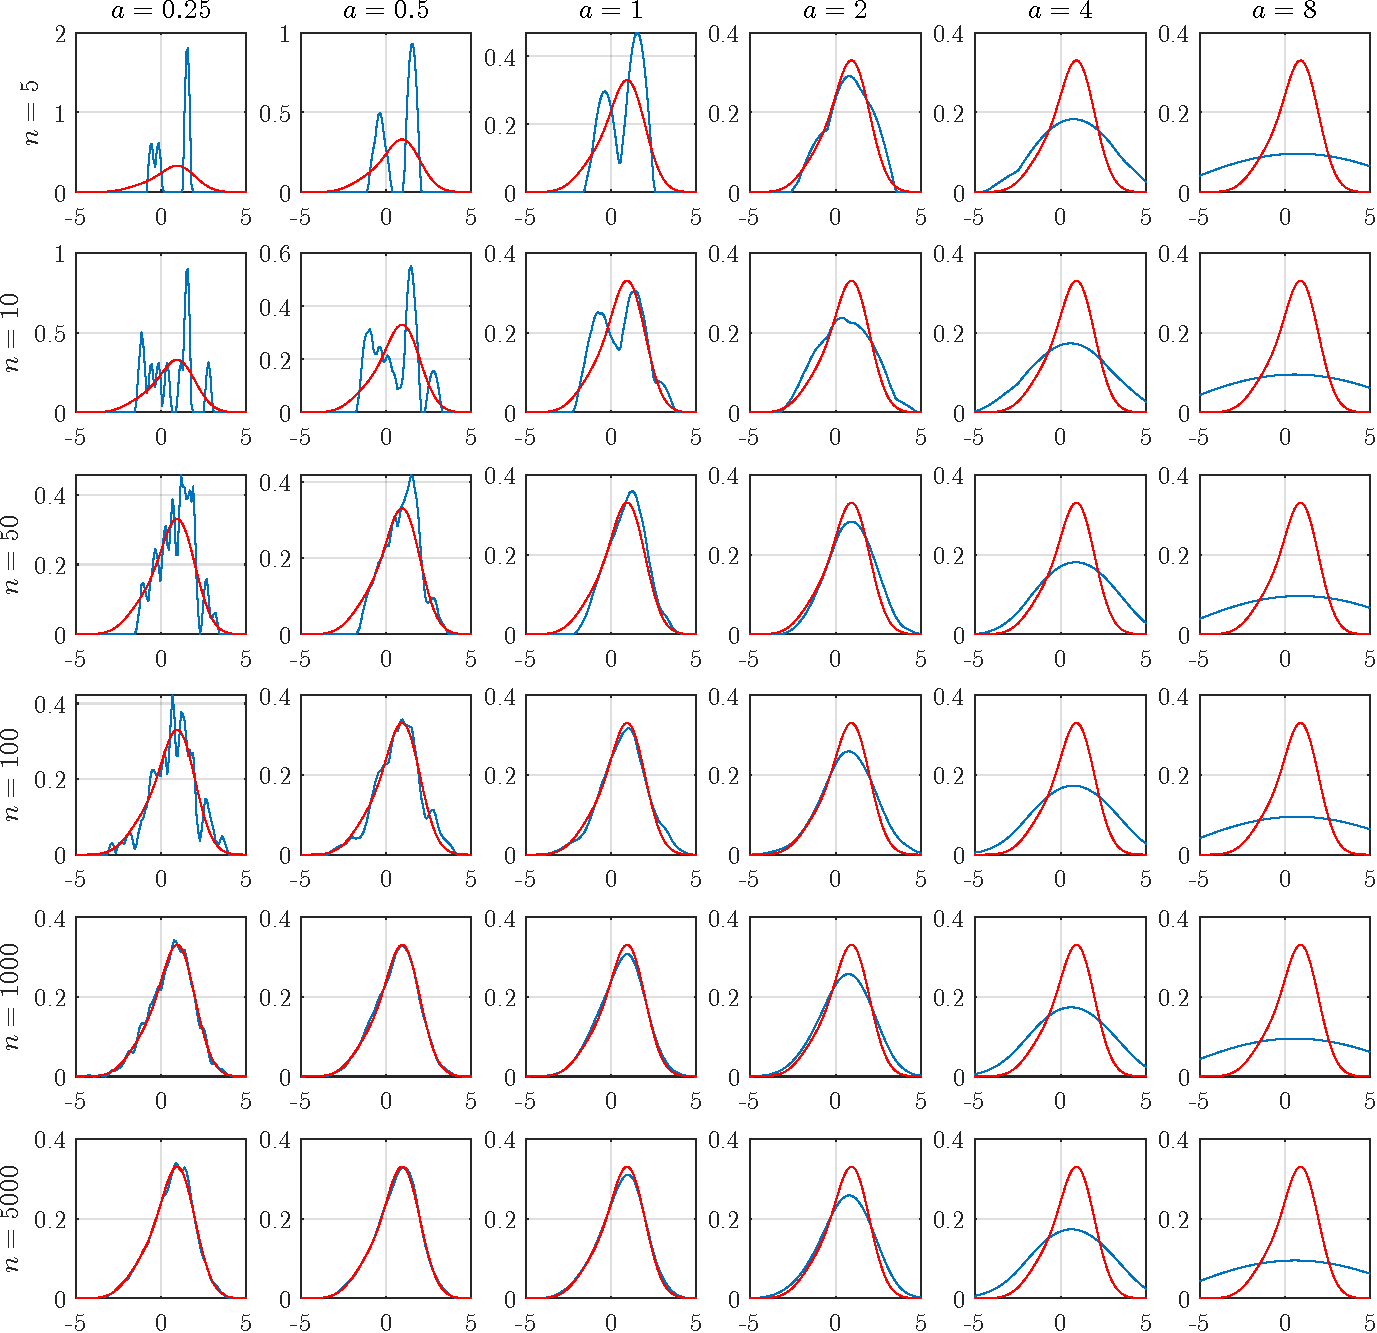
\includegraphics[width=0.9\textwidth]{cosineWindow.pdf}
  \caption{余弦估计}
  \label{fig:coswin}
\end{figure}

\begin{table}[htbp]
  \centering
  \begin{tabular}{l|cccccc}
  \hline
           & $a=0.25$ & $a=0.5$ & $a=1$  & $a=2$  & $a=4$  & $a=8$  \\ \hline
  $n=5$    & 0.0433   & 0.0195  & 0.0068 & 0.0045 & 0.0049 & 0.0106 \\
  $n=10$   & 0.0227   & 0.0104  & 0.0032 & 0.0022 & 0.0044 & 0.0106 \\
  $n=50$   & 0.0047   & 0.0021  & 0.0006 & 0.0009 & 0.0044 & 0.0106 \\
  $n=100$  & 0.0024   & 0.0009  & 0.0005 & 0.0009 & 0.0045 & 0.0106 \\
  $n=1000$ & 0.0002   & 0.0001  & 0.0001 & 0.0008 & 0.0044 & 0.0106 \\
  $n=5000$ & 0.0000   & 0.0000  & 0.0001 & 0.0008 & 0.0044 & 0.0106 \\ \hline
  \end{tabular}
  \caption{余弦估计均方误差期望}
  \label{tab:cosMeanMSE}
\end{table}

\begin{table}[htbp]
  \centering
  \begin{tabular}{l|cccccc}
    \hline
             & $a=0.25$   & $a=0.5$    & $a=1$      & $a=2$      & $a=4$      & $a=8$      \\ \hline
    $n=5$    & 2.2951e-04 & 9.5301e-05 & 1.5815e-05 & 1.9215e-05 & 1.2055e-06 & 4.0842e-08 \\
    $n=10$   & 6.0942e-05 & 2.9110e-05 & 2.7757e-06 & 3.3023e-06 & 2.0050e-07 & 1.4286e-08 \\
    $n=50$   & 3.2806e-06 & 1.3003e-06 & 1.8299e-07 & 2.7372e-07 & 4.0559e-08 & 3.9168e-09 \\
    $n=100$  & 5.7175e-07 & 1.3395e-07 & 1.0991e-07 & 1.0813e-07 & 4.0889e-08 & 1.5858e-09 \\
    $n=1000$ & 3.9053e-09 & 1.2351e-09 & 1.7076e-09 & 5.7179e-09 & 3.2295e-09 & 1.2545e-10 \\
    $n=5000$ & 1.4506e-39 & 1.4286e-39 & 1.4239e-38 & 3.6626e-37 & 1.0295e-36 & 9.5029e-36 \\ \hline
  \end{tabular}
  \caption{余弦估计均方误差方差}
  \label{tab:cosVarMSE}
\end{table}

取 $n=5,10,50,100,1000,5000$, $a=0.25,0.5,1,2,4,8$, 使用指数核函数
\begin{equation}
  K(x)=\frac{1}{2a}\exp\left(-\left\lvert\frac{x}{a}\right\rvert\right)
\end{equation} 
进行估计, 结果如图 \ref{fig:expwin} 所示, 图中红色曲线表示 $p(x)$. 对每一组给定的 $(n,a)$, 进行多次重复试验, 而后对多次试验得到的 $\epsilon(p_n)$ 数组计算均值和方差, 结果分别如表 \ref{tab:expMeanMSE} 和表 \ref{tab:expVarMSE} 所示.

\begin{figure}[htbp]
  \centering
  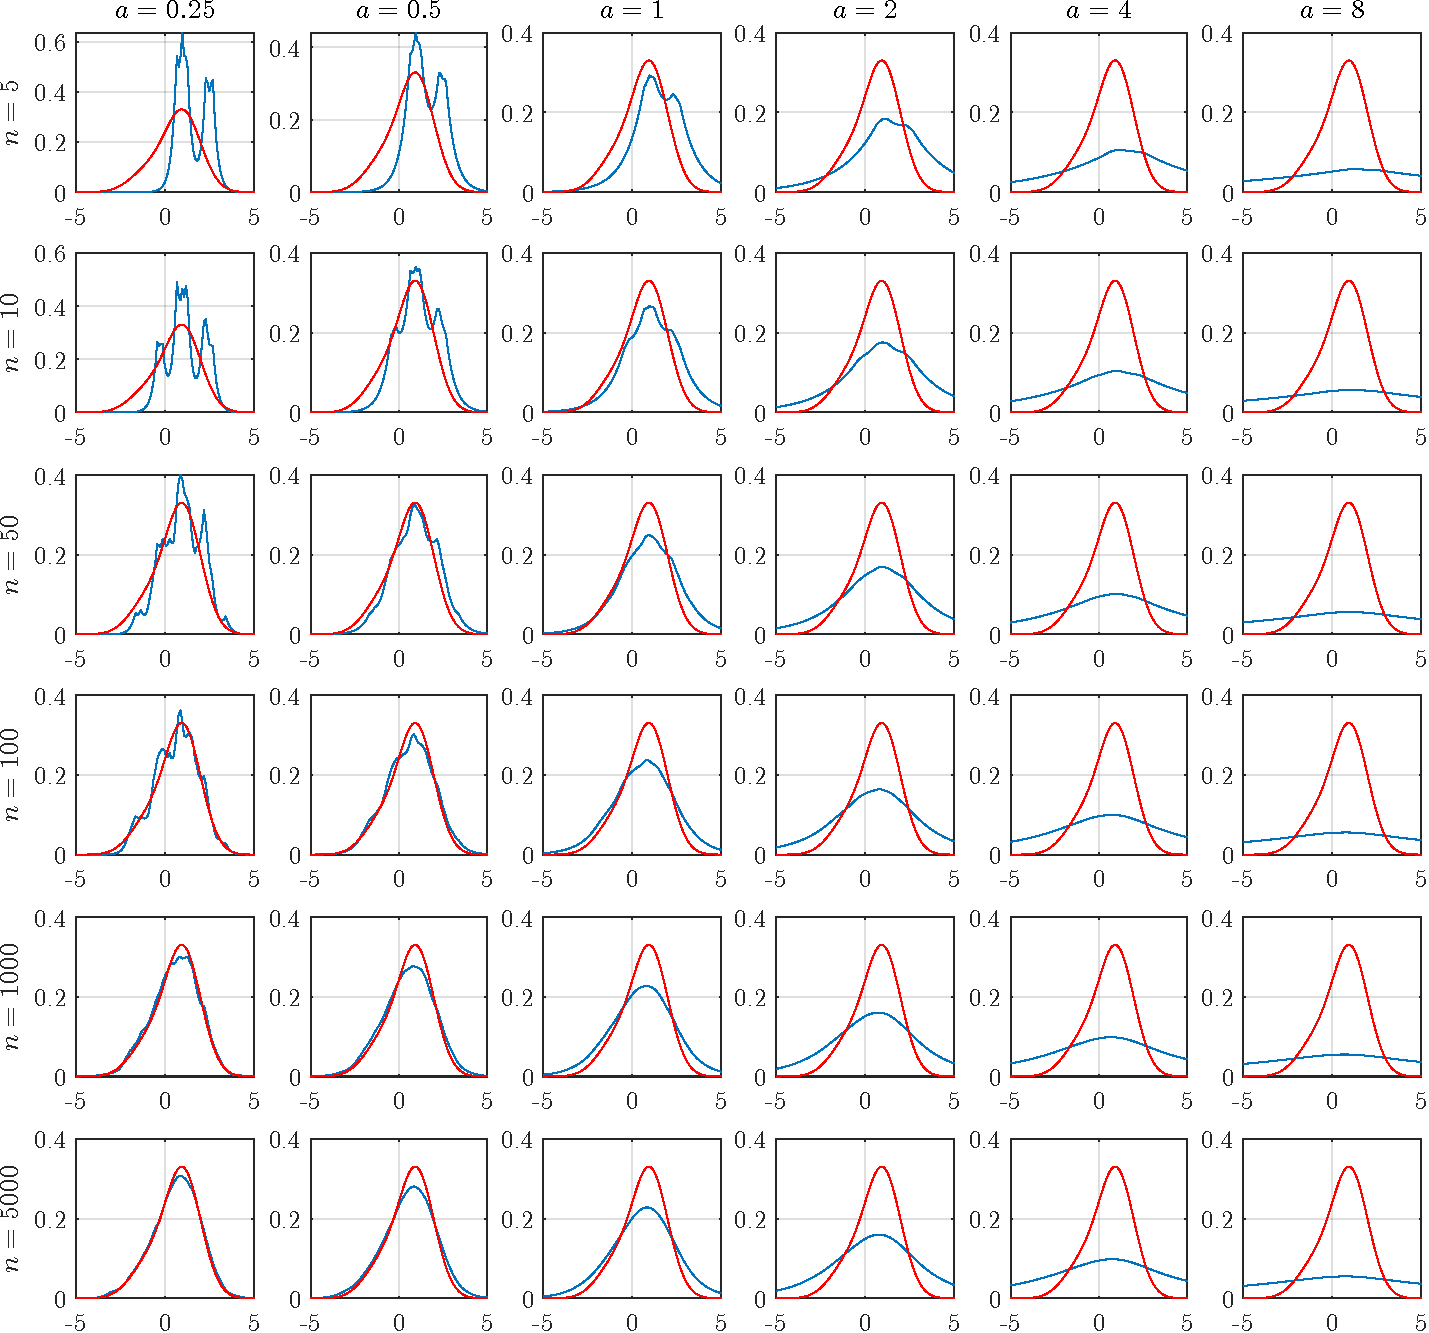
\includegraphics[width=0.9\textwidth]{exponentialWindow.pdf}
  \caption{指数估计}
  \label{fig:expwin}
\end{figure}

\begin{table}[htbp]
  \centering
  \begin{tabular}{l|cccccc}
  \hline
           & $a=0.25$ & $a=0.5$ & $a=1$  & $a=2$  & $a=4$  & $a=8$  \\ \hline
  $n=5$    & 0.0159   & 0.0043  & 0.0029 & 0.0049 & 0.0097 & 0.0139 \\
  $n=10$   & 0.0069   & 0.0034  & 0.0026 & 0.0050 & 0.0097 & 0.0139 \\
  $n=50$   & 0.0015   & 0.0009  & 0.0017 & 0.0049 & 0.0097 & 0.0140 \\
  $n=100$  & 0.0008   & 0.0006  & 0.0016 & 0.0049 & 0.0096 & 0.0140 \\
  $n=1000$ & 0.0001   & 0.0003  & 0.0016 & 0.0050 & 0.0096 & 0.0140 \\
  $n=5000$ & 0.0000   & 0.0003  & 0.0016 & 0.0049 & 0.0096 & 0.0140 \\ \hline
  \end{tabular}
  \caption{指数估计均方误差期望}
  \label{tab:expMeanMSE}
\end{table}

\begin{table}[htbp]
  \centering
  \begin{tabular}{l|cccccc}
  \hline
           & $a=0.25$   & $a=0.5$    & $a=1$      & $a=2$      & $a=4$      & $a=8$      \\ \hline
  $n=5$    & 4.4102e-05 & 4.6225e-06 & 3.6103e-06 & 7.1588e-07 & 6.2318e-07 & 5.3395e-08 \\
  $n=10$   & 4.9972e-06 & 5.7290e-06 & 1.8833e-06 & 8.6840e-07 & 3.0770e-07 & 2.0078e-08 \\
  $n=50$   & 8.6323e-07 & 1.6730e-07 & 3.5128e-07 & 1.9786e-07 & 4.7670e-08 & 5.5717e-09 \\
  $n=100$  & 9.7696e-08 & 1.1821e-07 & 1.8168e-07 & 8.9720e-08 & 1.5764e-08 & 1.6416e-09 \\
  $n=1000$ & 2.5749e-09 & 5.8766e-09 & 1.3514e-08 & 4.2008e-09 & 1.4476e-09 & 2.4628e-10 \\
  $n=5000$ & 7.1807e-39 & 1.7308e-37 & 6.2858e-37 & 4.9494e-36 & 1.1087e-36 & 3.6428e-36 \\ \hline
  \end{tabular}
  \caption{指数估计均方误差方差}
  \label{tab:expVarMSE}
\end{table}

最优参数与窗函数: 通过整体比较方窗, 高斯窗, 三角形窗, 余弦窗, 指数窗等5种类型窗函数的估计效果, 均方误差的期望和方差大小, 可以看出当窗宽 $a=0.5$ 且样本数为 $n=5000$ 时, 三角形窗的估计效果最好, 其均方误差均值 $6.4746\times10^{-6}$ 和方差 $8.1878\times10^{-40}$ 都是所有估计结果中最小的.

\chapter{EM 算法与高斯混合模型 GMM}

\section{EM 算法}

思想:用隐变量对缺失数据建模,迭代实现最大似然估计

数据:$X=\{ x_1,\dots,x_N\}$,隐变量 $Y$,完整数据 $Z=\left(X,Y \right)$

似然函数:
\begin{equation}
\begin{aligned}
  l(\theta)
  &=p(X|\theta)\\
  &=\sum_{y\in Y}p\left(X,y|\theta \right)
\end{aligned}
\end{equation}

对数似然函数:
\begin{equation}
\begin{aligned}
  L(\theta)
  &=\ln l(\theta)\\
  &=\ln \sum_{y\in Y}p\left(X,y|\theta \right)
\end{aligned}
\end{equation}

对数似然函数的下界:应用 Jensen 不等式于对数函数可得
\begin{equation}
\begin{aligned}
  L(\theta)
  &=\ln \sum_yp\left(X,y|\theta \right)\\
  &=\ln \sum_y\frac{q(y)p\left(X,y|\theta \right)}{q(y)}\\
  &\geqslant \sum_yq(y)\ln\frac{p\left(X,y|\theta \right)}{q(y)} \\
  &=\sum_yq(y)\ln p\left(X,y|\theta \right)-\sum_yq(y)\ln q(y)\\
  &:=F\left(q,\theta \right)
\end{aligned}
\end{equation}

迭代优化下界:初始化 $q_{\left[0 \right]},~\theta_{\left[0 \right]}$ 后反复迭代
\begin{equation}
\begin{aligned}
  q_{\left[k+1 \right]}&\gets \mathrm{argmax}_qF\left(q,\theta_{\left[k \right]} \right)\\
  \theta_{\left[k+1 \right]}&\gets \mathrm{argmax}_{\theta}F\left(q_{\left[k+1 \right]},\theta \right)
\end{aligned}
\end{equation}

\begin{figure}
  \centering
  \includegraphics[width=7cm]{1627808293080-3.1.jpg}
  \caption{迭代优化下界}
\end{figure}

期望:当 $q=p\left(y|X,\theta_{\left[k \right]} \right)$ 为后验概率时,$F\left(q,\theta_{\left[k \right]} \right)$ 达到最大
\begin{equation}
\begin{aligned}
  F\left(q,\theta \right)
  &=\sum_yq(y)\ln\frac{p\left(X,y|\theta \right)}{q(y)}\\
  &=\sum_yp\left(y|X,\theta \right)\ln\frac{p\left(y|X,\theta \right)p(X|\theta)}{p\left(y|X,\theta \right)} \\
  &=\sum_yp\left(y|X,\theta \right)\ln p(X|\theta)\\
  &=\ln p(X|\theta)\\
  &=L(\theta)
\end{aligned}
\end{equation}
\begin{equation}
\begin{aligned}
  F\left(q_{\left[k+1 \right]},\theta \right)=\sum_yq_{\left[k+1 \right]}(y)\ln p\left(X,y|\theta \right)-\sum_yq_{\left[k+1 \right]}(y)\ln q_{\left[k+1 \right]}(y)
\end{aligned}
\end{equation}

第二项不包含优化变量 $\theta$ 可忽略,代入 $q_{\left[k+1 \right]}(y)$ 并定义
\begin{equation}
\begin{aligned}
  Q\left(\theta_{\left[k \right]},\theta \right)&:=\sum_yp\left(y|X,\theta_{\left[k \right]} \right)\ln p\left(X,y|\theta \right)\\
  &=\mathbb{E} \left[\ln p\left(X,y|\theta \right)|X,\theta_{\left[ k \right]} \right]
\end{aligned}
\end{equation}

最大化:
\begin{equation}
\theta_{\left[k+1 \right]}\gets \mathrm{argmax}_{\theta}Q\left(\theta_{\left[k \right]},\theta \right)
\end{equation}

广义最大化:
\begin{equation}
\theta_{\left[k+1 \right]}\in \left\{ \theta_{\left[k+1 \right]}|Q\left(\theta_{\left[k \right]},\theta_{\left[k+1 \right]} \right)>Q\left(\theta_{\left[k \right]},\theta_{\left[k \right]} \right)\right\}
\end{equation}

\section{高斯混合模型 GMM}

隐变量:$Y=\left\{ y\in \mathbb{R} ^N \right\}$ 表示样本 $x_i$ 由第 $y_i$ 个高斯分布产生

混合模型:
\begin{equation}
p(X|\theta)=\Sigma_j\alpha_jp_j\left(X|\theta_j \right)
\end{equation}

其中
\begin{equation}
\Theta =\left\{ \alpha_j,\theta_j \right\},~\sum_j\alpha_j=1
\end{equation}

由独立同分布可得
\begin{equation}
\begin{aligned}
  p(X|\theta)
  &=\prod_ip\left(x_i|\Theta \right)\\
  &=\prod_i\sum_j\alpha_jp_j\left(x_i|\theta_j \right)
\end{aligned}
\end{equation}

对数似然函数:
\begin{equation}
\ln p(X|\theta)=\sum_i\ln \sum_j\alpha_jp_j\left(x_i|\theta_j \right)
\end{equation}

极大似然估计:
\begin{equation}
\nabla_{\Theta}\ln p(X|\theta)=0\Rightarrow \Theta
\end{equation}

结果与EM相同

EM 算法:
\begin{equation}
p\left(X,y|\Theta \right)=\prod_ip\left(x_i|y_i \right)p\left(y_i \right)
\end{equation}
\begin{equation}
\begin{aligned}
  \ln p\left(X,y|\Theta \right)
  &=\sum_i\ln p\left(x_i|y_i \right)p\left(y_i \right)\\
  &=\sum_i\ln \alpha_{y_i}p_{y_i}\left(x_i|\theta_{y_i} \right)
\end{aligned}
\end{equation}
\begin{equation}
\begin{aligned}
  p\left(y|X,\Theta ^g \right)
  &=\prod_ip\left(y_i|x_i,\Theta ^g \right)\\
  &=\prod_i\alpha_{y_i}^{g}\frac{p_{y_i}\left(x_i|\theta_{y_i}^{g} \right)}{p\left(x_i|\Theta ^g \right)}
\end{aligned}
\end{equation}
\begin{equation}
\begin{aligned}
  Q\left(\Theta ^g,\Theta \right)
  &=\sum_yp\left(y|X,\Theta ^g \right)\ln p\left(X,y|\Theta \right)\\
  &=\sum_j\sum_i\ln \left(\alpha_jp_j\left(x_i|\theta_j \right)\right)p\left(j|x_i,\Theta ^g \right)\\
  &=\sum_j\sum_ip\left(j|x_i,\Theta ^g \right)\left[\ln \alpha_j+\ln p_j\left(x_i|\theta_j \right)\right]
\end{aligned}
\end{equation}

$\alpha_j$ 与 $\theta_j$ 解耦可分别优化,由 $\sum_i\alpha_i=1$ 及梯度条件解得
\begin{equation}
\begin{aligned}
  \alpha_{j}^{\mathrm{new}}&=\frac{1}{N}\sum_ip\left(j|x_i,\Theta ^g \right)\\ 
  \mu_{j}^{\mathrm{new}}&=\frac{1}{N\alpha_{j}^{\mathrm{new}}}\sum_ix_ip\left(j|x_i,\Theta ^g \right)\\
  \Sigma_{j}^{\mathrm{new}}&=\frac{1}{N\alpha_{j}^{\mathrm{new}}}\sum_ip\left(j|x_i,\Theta ^g \right)\left(x_i-\mu_{j}^{\mathrm{new}} \right)\left(x_i-\mu_{j}^{\mathrm{new}} \right)^{\top}
\end{aligned}
\end{equation}

若限制各成分的协方差矩阵均相同,则 M 步需要修改为
\begin{equation}
\Sigma ^{\mathrm{new}}=\sum_{j}\sum_i\frac{p\left(j|x_i,\Theta ^g \right)\left(x_i-\mu_{j}^{\mathrm{new}} \right)\left(x_i-\mu_{j}^{\mathrm{new}} \right)^{\top}}{N\sum_j\alpha_{j}^{\mathrm{new}}}
\end{equation}

例题:三维数据点,偶数点的第3维数据缺失,令 $x_{i3},~i\in E$ 为隐变量,
\begin{equation}
x_i=\left[x_{i1},x_{i2},x_{i3} \right] ^{\top}
\end{equation}

则对数似然函数为
\begin{equation}
\begin{aligned}
  L(\theta)
  &=\sum_{i\in O}\ln p\left(x_{i1},x_{i2},x_{i3}|\theta \right)+\sum_{i\in E}\ln p\left(x_{i1},x_{i2}|\theta \right)\\
  &=\sim +\sum_{i\in E}\ln \int_{-\infty}^{+\infty}p\left(x_{i1},x_{i2},x_{i3}|\theta \right)\mathrm{d}x_{i3}\\
  &=\sim +\sum_{i\in E}\ln \int_{-\infty}^{+\infty}\frac{q\left(x_{i3} \right)p\left(x_{i1},x_{i2},x_{i3}|\theta \right)}{q\left(x_{i3} \right)}\mathrm{d}x_{i3}\\
  &\geqslant \sim +\sum_{i\in E}\int_{-\infty}^{+\infty}q\left(x_{i3} \right)\ln\frac{p\left(x_{i1},x_{i2},x_{i3}|\theta \right)}{q\left(x_{i3} \right)} \mathrm{d}x_{i3}
\end{aligned}
\end{equation}
\begin{equation}
Q\left(\theta_{\left[k \right]},\theta \right)=\sim +\sum_{i\in E}\int_{-\infty}^{+\infty}p\left(x_{i3}|x_{i1},x_{i2},\theta_{\left[k \right]} \right)\ln p\left(\vec{x}_i|\theta \right)\mathrm{d}x_{i3}
\end{equation}

\section{习题}


1. In this problem you will see connections between the EM algorithm and gradient descent. Consider a GMM with known mixture weight $\pi_k$ and spherical covariances (but the radius of spheres might be different). Its log likelihood is given by
\begin{equation}
	l\left(\left\{\mu_k,\sigma_k^2\right\}_{k=1}^K\right) = \sum_{i=1}^n\log\left(\sum_{k=1}^K\pi_k N(x_i|\mu_k,\sigma_k^2I)\right).
\end{equation}

A maximization algorithm based on gradient descent should be something like:
\begin{itemize}
	\item Initialize $\mu_k$ and $\sigma_k^2$, $k \in\{1,2,\cdots,K\}$. Set the iteration counter $t\leftarrow1$.
	\item Repeat the following until convergence:
	\begin{itemize}
		\item For $k=1,2,\cdots ,K$,
      \begin{equation}
        \mu_k^{(t+1)}\leftarrow\mu_k^{(t)}+\eta_k^{(t)}\nabla_{\mu_k}l\left(\left\{\mu_k^{(t)},(\sigma_k ^2)^{(t)}\right\}_{k=1}^K\right)
      \end{equation}
		\item For $k=1,2,\cdots ,K$,
      \begin{equation}
        (\sigma_k ^2)^{(t+1)} \leftarrow (\sigma_k ^2)^{(t)}+s_k^{(t)}\nabla_{\sigma_k^2}l\left(\left\{\mu_k^{(t+1)},(\sigma_k ^2)^{(t)}\right\}_{k=1}^K\right)
      \end{equation}
		\item Increase the iteration counter $t\leftarrow t+1$.
	\end{itemize}
\end{itemize}

Please prove that with properly chosen step size $\eta_k^{(t)}$ and $s_k^{(t)}$, the above gradient descent algorithm is essentially equivalent to the following \emph{modified} EM algorithm:
\begin{itemize}
	\item Initialize $\mu_k$ and $\sigma_k^2$, $k \in \{1,2,\cdots ,K\}$. Set the iteration counter $t\leftarrow1$.
	\item Repeat the following until convergence:
	\begin{itemize}
		\item E-step:
      \begin{equation}
        \tilde{z}_{ik}^{(t+0.5)} \leftarrow P\left(x_i\in \mathrm{cluster}_k \Big| \left\{\mu_j^{(t)},(\sigma_j^2)^{(t)}\right\}_{j=1}^K,x_i\right)
      \end{equation}
		\item M-step:
      \begin{equation}
        \left\{\mu_k^{(t+1)}\right\}_{k=1}^K \leftarrow \argmax_{\{\mu_k\}_{k=1}^K} \sum_{i=1}^n\sum_{k=1}^K \tilde{z}_{ik}^{(t+0.5)} \left[\log N\left(x_i\Big|\mu_k,(\sigma_k^2)^{(t)}I\right)+\log\pi_k\right]
      \end{equation}
		\item E-step:
      \begin{equation}
        \tilde{z}_{ik}^{(t+1)} \leftarrow P\left(x_i \in \mathrm{cluster}_k \Big| \left\{\mu_j^{(t+1)},(\sigma_j^2)^{(t)}\right\}_{j=1}^K,x_i\right)
      \end{equation}
		\item M-step:
      \begin{equation}
        \left\{(\sigma_k^2)^{(t+1)}\right\}_{k=1}^K \leftarrow \argmax_{\{\sigma_k^2\}_{k=1}^K} \sum_{i=1}^n \sum_{k=1}^K \tilde{z}_{ik}^{(t+1)} \left[\log N\left(x_i\Big|\mu_k^{(t+1)},\sigma_k^2I\right)+\log \pi_k \right]
      \end{equation}
		\item Increase the iteration counter $t\leftarrow t+1$.
	\end{itemize}
\end{itemize}

The main modification is inserting an extra E-step between the M-step for $\mu_k$'s and the M-step for $\sigma_k^2$'s.

\emph{Hint:} Find the exact algebraic form of step size $\eta_k^{(t)}$ and $s_k^{(t)}$ from M-step.

解: 设样本点 $x_i$ 的维数为 $d$, 则正态分布概率密度为
\begin{equation}
  N(x_i|\mu_k,\sigma_k^2I)=\frac{1}{(2\pi\sigma_k^2)^{d/2}}\exp\left[-\frac{1}{2\sigma_k^2}(x_i-\mu_k)^{\top}(x_i-\mu_k)\right]
\end{equation}

其对 $\mu_k$ 的梯度为
\begin{equation}
  \nabla_{\mu_k}N(x_i|\mu_k,\sigma_k^2I)
  =N(x_i|\mu_k,\sigma_k^2I)\frac{x_i-\mu_k}{\sigma_k^2}
\end{equation}

对 $\sigma_k^2$ 的梯度为
\begin{equation}
  \begin{aligned}
    \nabla_{\sigma_k^2}N(x_i|\mu_k,\sigma_k^2I)
    &=N(x_i|\mu_k,\sigma_k^2I)\left[-\frac{d}{2\sigma_k^2}+\frac{1}{2(\sigma_k^2)^2}(x_i-\mu_k)^{\top}(x_i-\mu_k)\right]
  \end{aligned}
\end{equation}

所以, 似然函数对 $\mu_k$ 的梯度为
\begin{equation}
  \begin{aligned}
    \nabla_{\mu_k}l\left(\left\{\mu_k,\sigma_k ^2\right\}_{k=1}^K\right)
    &=\nabla_{\mu_k} \sum_{i=1}^n \log\left(\sum_{k=1}^K\pi_k N(x_i|\mu_k,\sigma_k^2I)\right)\\
    &=\sum_{i=1}^n\frac{\pi_k N(x_i|\mu_k,\sigma_k^2I)}{\displaystyle\sum_{k=1}^K\pi_k N(x_i|\mu_k,\sigma_k^2I)}\frac{x_i-\mu_k}{\sigma_k^2}\\
  \end{aligned}
\end{equation}

似然函数对 $\sigma_k^2$ 的梯度为
\begin{equation}
  \begin{aligned}
    \nabla_{\sigma_k^2}l\left(\left\{\mu_k,\sigma_k^2\right\}_{k=1}^K\right)
    &=\nabla_{\sigma_k^2} \sum_{i=1}^n \log\left(\sum_{k=1}^K\pi_k N(x_i|\mu_k,\sigma_k^2I)\right)\\
    &=\sum_{i=1}^n \frac{\pi_k N(x_i|\mu_k,\sigma_k^2I)}{\displaystyle\sum_{k=1}^K\pi_k N(x_i|\mu_k,\sigma_k^2I)}\left[-\frac{d}{2\sigma_k^2}+\frac{1}{2(\sigma_k^2)^2}(x_i-\mu_k)^{\top}(x_i-\mu_k)\right]\\
  \end{aligned}
\end{equation}

对改进 EM 算法, 第一个 E-step: 由 Bayes 公式可得
\begin{equation}
  \begin{aligned}
    \tilde{z}_{ik}^{(t+0.5)} 
    &=P\left(x_i\in \mathrm{cluster}_k \Big| \left\{\mu_j^{(t)},(\sigma_j^2)^{(t)}\right\}_{j=1}^K,x_i\right)\\
    &=\frac{\pi_k N\left(x_i\Big|\mu_k^{(t)},(\sigma_k^2)^{(t)}I\right)}{\displaystyle\sum_{k=1}^K\pi_k N\left(x_i\Big|\mu_k^{(t)},(\sigma_k^2)^{(t)}I\right)}
  \end{aligned}
\end{equation}

第一个 M-step: 令
\begin{equation}
    Q^{(t+0.5)}\triangleq\sum_{i=1}^n\sum_{k=1}^K \tilde{z}_{ik}^{(t+0.5)} \left[\log N\left(x_i\Big|\mu_k,(\sigma_k^2)^{(t)}I\right)+\log\pi_k\right]
\end{equation}

则其对 $\mu_k$ 的梯度为
\begin{equation}
  \begin{aligned}
    \frac{\partial Q^{(t+0.5)}}{\partial \mu_k}
    &=\sum_{i=1}^n\tilde{z}_{ik}^{(t+0.5)}\frac{N\left(x_i\Big|\mu_k,(\sigma_k^2)^{(t)}I\right)}{N\left(x_i\Big|\mu_k,(\sigma_k^2)^{(t)}I\right)}\frac{x_i-\mu_k}{(\sigma_k^2)^{(t)}}\\
    &=\sum_{i=1}^n\tilde{z}_{ik}^{(t+0.5)}\frac{x_i-\mu_k}{(\sigma_k^2)^{(t)}}\\
    &=\frac{1}{(\sigma_k^2)^{(t)}}\left(\sum_{i=1}^n\tilde{z}_{ik}^{(t+0.5)}x_i-\sum_{i=1}^n\tilde{z}_{ik}^{(t+0.5)}\mu_k\right)
  \end{aligned}
\end{equation}

令此梯度为 0, 则有
\begin{equation}
  \mu_k^{(t+1)}=\frac{\displaystyle\sum_{i=1}^n\tilde{z}_{ik}^{(t+0.5)}x_i}{\displaystyle\sum_{i=1}^n\tilde{z}_{ik}^{(t+0.5)}}
\end{equation}

对梯度下降算法, $\mu_k^{(t+1)}$ 为
\begin{equation}
  \begin{aligned}
    \mu_k^{(t+1)}
    &=\mu_k^{(t)}+\eta_k^{(t)}\nabla_{\mu_k}l\left(\left\{\mu_k^{(t)},(\sigma_k ^2)^{(t)}\right\}_{k=1}^K\right)\\
    &=\mu_k^{(t)}+\eta_k^{(t)}\sum_{i=1}^n\frac{\pi_k N\left(x_i\Big|\mu_k^{(t)},(\sigma_k^2)^{(t)}I\right)}{\displaystyle\sum_{k=1}^K\pi_k N\left(x_i\Big|\mu_k^{(t)},(\sigma_k^2)^{(t)}I\right)}\frac{x_i-\mu_k^{(t)}}{(\sigma_k ^2)^{(t)}}\\
    &=\mu_k^{(t)}+\eta_k^{(t)}\sum_{i=1}^n\tilde{z}_{ik}^{(t+0.5)}\frac{x_i-\mu_k^{(t)}}{(\sigma_k ^2)^{(t)}}\\
  \end{aligned}
\end{equation}

令梯度下降算法得到的 $\mu_k^{(t+1)}$ 与 EM 算法得到的结果相等, 则有
\begin{equation}
  \frac{\displaystyle\sum_{i=1}^n\tilde{z}_{ik}^{(t+0.5)}x_i}{\displaystyle\sum_{j=1}^n\tilde{z}_{jk}^{(t+0.5)}}
  =\mu_k^{(t)}+\eta_k^{(t)}\sum_{i=1}^n\tilde{z}_{ik}^{(t+0.5)}\frac{x_i-\mu_k^{(t)}}{(\sigma_k ^2)^{(t)}}
\end{equation}

通分有
\begin{equation}
  \sum_{i=1}^n\tilde{z}_{ik}^{(t+0.5)}x_i
  =\sum_{j=1}^n\tilde{z}_{jk}^{(t+0.5)}\mu_k^{(t)}+\sum_{j=1}^n\tilde{z}_{jk}^{(t+0.5)}\eta_k^{(t)}\sum_{i=1}^n\tilde{z}_{ik}^{(t+0.5)}\frac{x_i-\mu_k^{(t)}}{(\sigma_k ^2)^{(t)}}
\end{equation}

移项可得
\begin{equation}
  \sum_{i=1}^n\tilde{z}_{ik}^{(t+0.5)}\left(x_i-\mu_k^{(t)}\right)
  =\frac{\eta_k^{(t)}\displaystyle\sum_{j=1}^n\tilde{z}_{jk}^{(t+0.5)}}{(\sigma_k ^2)^{(t)}}\sum_{i=1}^n\tilde{z}_{ik}^{(t+0.5)}\left(x_i-\mu_k^{(t)}\right)
\end{equation}

即
\begin{equation}
  \frac{\eta_k^{(t)}\displaystyle\sum_{j=1}^n\tilde{z}_{jk}^{(t+0.5)}}{(\sigma_k ^2)^{(t)}}=1
\end{equation}

所以
\begin{equation}
  \eta_k^{(t)}=\frac{(\sigma_k ^2)^{(t)}}{\displaystyle\sum_{j=1}^n\tilde{z}_{jk}^{(t+0.5)}}
\end{equation}

对改进 EM 算法, 第二个 E-step: 由 Bayes 公式可得
\begin{equation}
  \begin{aligned}
    \tilde{z}_{ik}^{(t+1)} 
    &=P\left(x_i\in \mathrm{cluster}_k \Big| \left\{\mu_j^{(t+1)},(\sigma_j^2)^{(t)}\right\}_{j=1}^K,x_i\right)\\
    &=\frac{\pi_k N\left(x_i\Big|\mu_k^{(t+1)},(\sigma_k^2)^{(t)}I\right)}{\displaystyle\sum_{k=1}^K\pi_k N\left(x_i\Big|\mu_k^{(t+1)},(\sigma_k^2)^{(t)}I\right)}
  \end{aligned}
\end{equation}

第二个 M-step: 令
\begin{equation}
    Q^{(t+1)}\triangleq\sum_{i=1}^n\sum_{k=1}^K \tilde{z}_{ik}^{(t+1)} \left[\log N\left(x_i\Big|\mu_k^{(t+1)},\sigma_k^2I\right)+\log\pi_k\right]
\end{equation}

则其对 $\sigma_k^2$ 的梯度为
\begin{equation}
  \begin{aligned}
    \frac{\partial Q^{(t+1)}}{\partial \sigma_k^2}
    &=\sum_{i=1}^n\tilde{z}_{ik}^{(t+1)}\frac{N\left(x_i\Big|\mu_k^{(t+1)},\sigma_k^2I\right)}{N\left(x_i\Big|\mu_k^{(t+1)},\sigma_k^2I\right)}\left[-\frac{d}{2\sigma_k^2}+\frac{1}{2(\sigma_k^2)^2}\left(x_i-\mu_k^{(t+1)}\right)^{\top}\left(x_i-\mu_k^{(t+1)}\right)\right]\\
    &=\sum_{i=1}^n\tilde{z}_{ik}^{(t+1)}\left[-\frac{d}{2\sigma_k^2}+\frac{1}{2(\sigma_k^2)^2}\left(x_i-\mu_k^{(t+1)}\right)^{\top}\left(x_i-\mu_k^{(t+1)}\right)\right]\\
    &=\frac{1}{2(\sigma_k^2)^2}\left[\sum_{i=1}^n\tilde{z}_{ik}^{(t+1)}\left\|x_i-\mu_k^{(t+1)}\right\|^2-\sigma_k^2d\sum_{i=1}^n\tilde{z}_{ik}^{(t+1)}\right]
  \end{aligned}
\end{equation}

令此梯度为 0, 则有
\begin{equation}
  (\sigma_k^2)^{(t+1)}=\frac{\displaystyle\sum_{i=1}^n\tilde{z}_{ik}^{(t+1)}\left\|x_i-\mu_k^{(t+1)}\right\|^2}{\displaystyle d\sum_{i=1}^n\tilde{z}_{ik}^{(t+1)}}
\end{equation}

对梯度下降算法, $(\sigma_k^2)^{(t+1)}$ 为
\begin{equation}
  \begin{aligned}
    (\sigma_k^2)^{(t+1)}
    &=(\sigma_k ^2)^{(t)}+s_k^{(t)}\nabla_{\sigma_k^2}l\left(\left\{\mu_k^{(t+1)},(\sigma_k^2)^{(t)}\right\}_{k=1}^K\right)\\
    &=(\sigma_k^2)^{(t)}+s_k^{(t)}\sum_{i=1}^n \frac{\pi_k N\left(x_i\Big|\mu_k^{(t+1)},(\sigma_k^2)^{(t)}I\right)}{\displaystyle\sum_{k=1}^K\pi_k N\left(x_i\Big|\mu_k^{(t+1)},(\sigma_k^2)^{(t)}I\right)}\left[-\frac{d}{2(\sigma_k^2)^{(t)}}+\frac{\left\|x_i-\mu_k^{(t+1)}\right\|^2}{2\big[(\sigma_k^2)^{(t)}\big]^2}\right]\\
    &=(\sigma_k ^2)^{(t)}+s_k^{(t)}\sum_{i=1}^n \tilde{z}_{ik}^{(t+1)}\left[-\frac{d}{2(\sigma_k^2)^{(t)}}+\frac{1}{2\big[(\sigma_k^2)^{(t)}\big]^2}\left\|x_i-\mu_k^{(t+1)}\right\|^2\right]\\
  \end{aligned}
\end{equation}

令梯度下降算法得到的 $(\sigma_k^2)^{(t+1)}$ 与 EM 算法得到的结果相等, 则有
\begin{equation}
  \frac{\displaystyle\sum_{i=1}^n\tilde{z}_{ik}^{(t+1)}\left\|x_i-\mu_k^{(t+1)}\right\|^2}{\displaystyle d\sum_{j=1}^n\tilde{z}_{jk}^{(t+1)}}
  =(\sigma_k ^2)^{(t)}+s_k^{(t)}\sum_{i=1}^n \tilde{z}_{ik}^{(t+1)}\left[-\frac{d}{2(\sigma_k^2)^{(t)}}+\frac{1}{2\big[(\sigma_k^2)^{(t)}\big]^2}\left\|x_i-\mu_k^{(t+1)}\right\|^2\right]
\end{equation}

通分并移项可得
\begin{equation}
  \sum_{i=1}^n\tilde{z}_{ik}^{(t+1)}\left(\left\|x_i-\mu_k^{(t+1)}\right\|^2-d(\sigma_k ^2)^{(t)}\right)
  =\frac{\displaystyle s_k^{(t)}d\sum_{j=1}^n\tilde{z}_{jk}^{(t+1)}}{2\big[(\sigma_k^2)^{(t)}\big]^2}\sum_{i=1}^n\tilde{z}_{ik}^{(t+1)}\left(\left\|x_i-\mu_k^{(t+1)}\right\|^2-d(\sigma_k ^2)^{(t)}\right)
\end{equation}

即
\begin{equation}
  \frac{\displaystyle s_k^{(t)}d\sum_{j=1}^n\tilde{z}_{jk}^{(t+1)}}{2\big[(\sigma_k^2)^{(t)}\big]^2}=1
\end{equation}

所以
\begin{equation}
  s_k^{(t)}=\frac{2\big[(\sigma_k^2)^{(t)}\big]^2}{\displaystyle d\sum_{j=1}^n\tilde{z}_{jk}^{(t+1)}}
\end{equation}

综上所述, 若取步长分别为
\begin{equation}
  \eta_k^{(t)}=\frac{(\sigma_k ^2)^{(t)}}{\displaystyle\sum_{j=1}^n\tilde{z}_{jk}^{(t+0.5)}},\quad s_k^{(t)}=\frac{2\big[(\sigma_k^2)^{(t)}\big]^2}{\displaystyle d\sum_{j=1}^n\tilde{z}_{jk}^{(t+1)}}
\end{equation}

则梯度下降算法与改进 EM 算法本质上是等价的.

2. The EM algorithm that we talked about in class was for solving a maximum likelihood estimation problem in which we wished to maximize
\begin{equation}
  \prod_{i = 1}^mp(x^{(i)}|\theta) = \prod_{i = 1}^m \sum_{z^{(i)}}p(x^{(i)},z^{(i)}|\theta)
\end{equation}
where $x^{(i)}$ were visible variables, $z^{(i)}$ were hidden variables and $m$ was the number of samples. Suppose we are working in a Bayesian framework, and wanted to find the MAP estimate of the parameters $\theta$ by maximizing
\begin{equation}
  \left(\prod_{i = 1}^mp(x^{(i)}|\theta)\right)p(\theta) = \left(\prod_{i = 1}^m \sum_{z^{(i)}}p(x^{(i)},z^{(i)}|\theta)\right)p(\theta)
  \label{eq:llhmap}
\end{equation}

Here, $p(\theta)$ is our prior on the parameters. Please generalize the EM algorithm to work for MAP estimation. You may assume that $\log p(x,z|\theta)$ and $\log p(\theta)$ are both concave in $\theta$, so that the M-step is tractable if it requires only maximizing a linear combination of these quantities. (This roughly corresponds to assuming that MAP estimation is tractable when $x, z$ is fully observed, just like in the frequentist case where we considered examples in which maximum likelihood estimation was easy if $x, z$ was fully observed.)

Make sure your M-step is tractable, and also prove that $\displaystyle\left(\prod_{i = 1}^mp(x^{(i)}|\theta)\right)p(\theta)$ (viewed as a function of $\theta$) monotonically increases with each iteration of your algorithm.

解: 令 $X=\left\{x^{(1)},x^{(2)},\cdots,x^{(m)}\right\}$, 对式 (\ref{eq:llhmap}) 取自然对数可得
\begin{equation}
  \begin{aligned}
    \tilde{H}(\theta)
    &=\log\big[p(X|\theta)p(\theta)\big]\\
    &=\log\left[\left(\prod_{i = 1}^mp(x^{(i)}|\theta)\right)p(\theta)\right]\\
    &=\log\left[\left(\prod_{i = 1}^m \sum_{z^{(i)}}p(x^{(i)},z^{(i)}|\theta)\right)p(\theta)\right]\\
    &=\sum_{i=1}^m\log\sum_{z^{(i)}}p\left(x^{(i)},z^{(i)}|\theta\right)+\log p(\theta)\\
  \end{aligned}
\end{equation}

引入隐变量分布 $q(\cdot)$, 由 Jensen 不等式可得
\begin{equation}
  \tilde{H}(\theta)
  \gs\sum_{i=1}^m\sum_{z^{(i)}}q(z^{(i)})\log p\left(x^{(i)},z^{(i)}|\theta\right)-\sum_{i=1}^m\sum_{z^{(i)}}q(z^{(i)})\log q(z^{(i)})+\log p(\theta)
  \triangleq \tilde{F}(q,\theta)
\end{equation}

直接优化 $\tilde{H}(\theta)$ 可能是很困难的, 所以我们转而优化 $\tilde{H}(\theta)$ 的下界函数 $\tilde{F}(q,\theta)$. 优化函数 $\tilde{F}(q,\theta)$ 可能也是比较困难的, 因此我们采用一种简单的迭代算法对 $\tilde{F}(q,\theta)$ 寻优, 首先对变量 $q,~\theta$ 初始化, 然后固定变量 $\theta_{[k]}$ 寻找能够最大化函数 $\tilde{F}(q,\theta_{[k]})$ 的参数 $q_{[k+1]}$, 再固定参数 $q_{[k+1]}$ 寻找能够最大化函数 $\tilde{F}(q_{[k+1]},\theta)$ 的参数 $\theta_{[k+1]}$, 即反复执行下面的两个步骤:
\begin{equation}
  q_{[k+1]}\leftarrow\argmax_{q}\tilde{F}(q,\theta_{[k]})
  \label{eq:estep}
\end{equation}
\begin{equation}
  \theta_{[k+1]}\leftarrow\argmax_{\theta}\tilde{F}(q_{[k+1]},\theta)
\end{equation}

当 $q_{[k+1]}(z^{(i)})=p(z^{(i)}|x^{(i)},\theta_{[k]})$ 时, 式 (\ref{eq:estep}) 取到最大值, 因为此时有
\begin{equation}
  \begin{aligned}
    \tilde{F}(q_{[k+1]},\theta_{[k]})
    &=\sum_{i=1}^m\sum_{z^{(i)}}q_{[k+1]}(z^{(i)})\log \frac{p\left(x^{(i)},z^{(i)}|\theta_{[k]}\right)}{q_{[k+1]}(z^{(i)})}+\log p(\theta_{[k]})\\
    &=\sum_{i=1}^m\sum_{z^{(i)}}p(z^{(i)}|x^{(i)},\theta_{[k]})\log \frac{p(z^{(i)}|x^{(i)},\theta_{[k]})p(x^{(i)}|\theta_{[k]})}{p(z^{(i)}|x^{(i)},\theta_{[k]})}+\log p(\theta_{[k]})\\
    &=\sum_{i=1}^m\sum_{z^{(i)}}p(z^{(i)}|x^{(i)},\theta_{[k]})\log p(x^{(i)}|\theta_{[k]})+\log p(\theta_{[k]})\\
    &=\sum_{i=1}^m\log p(x^{(i)}|\theta_{[k]})+\log p(\theta_{[k]})\\
    &=\log\left[\left(\prod_{i = 1}^mp(x^{(i)}|\theta_{[k]})\right)p(\theta_{[k]})\right]\\
    &=\tilde{H}(\theta_{[k]})
  \end{aligned}
  \label{eq:posterior}
\end{equation}

当 $q_{[k+1]}(z^{(i)})=p(z^{(i)}|x^{(i)},\theta_{[k]})$ 时, 
\begin{equation}
  \tilde{F}(q_{[k+1]},\theta)=\sum_{i=1}^m\sum_{z^{(i)}}q_{[k+1]}(z^{(i)})\log p\left(x^{(i)},z^{(i)}|\theta\right)-\sum_{i=1}^m\sum_{z^{(i)}}q_{[k+1]}(z^{(i)})\log q_{[k+1]}(z^{(i)})+\log p(\theta)
\end{equation}

由于第二项不包含需要优化的变量 $\theta$, 则可定义
\begin{equation}
  \tilde{Q}(\theta_{[k]},\theta)=\sum_{i=1}^m\sum_{z^{(i)}}p(z^{(i)}|x^{(i)},\theta_{[k]})\log p\left(x^{(i)},z^{(i)}|\theta\right)+\log p(\theta)
\end{equation}

假设 $\log p(x,z|\theta)$ 和 $\log p(\theta)$ 都是 $\theta$ 的凹函数, 则最大化函数 $\tilde{Q}$ 是一个无约束的凸优化问题, 即 M-step 是容易处理的 (tractable).

综上, 广义 EM 算法为:
\begin{itemize}
  \item 初始化变量 $q,~\theta$
  \item E 步骤, 计算函数 
    \begin{equation}
      \tilde{Q}(\theta_{[k]},\theta)=\sum_{i=1}^m\sum_{z^{(i)}}p(z^{(i)}|x^{(i)},\theta_{[k]})\log p\left(x^{(i)},z^{(i)}|\theta\right)+\log p(\theta)
    \end{equation}
  \item M 步骤, 
    \begin{equation}
      \theta_{[k+1]}\leftarrow\argmax_{\theta}\tilde{Q}(\theta_{[k]},\theta)
    \end{equation}
  \item 如果算法收敛则停止, 否则回到 E 步骤.
\end{itemize}

下面证明在广义 EM 算法下, $\displaystyle\left(\prod_{i = 1}^mp(x^{(i)}|\theta)\right)p(\theta)$ 作为 $\theta$ 的函数的单调性. 由式 (\ref{eq:posterior}) 并结合广义 EM 算法不断迭代求最大值可知
\begin{equation}
  \tilde{H}(\theta_{[k]})=\tilde{F}(q_{[k+1]},\theta_{[k]})\ls\tilde{F}(q_{[k+1]},\theta_{[k+1]})\ls\tilde{F}(q_{[k+2]},\theta_{[k+1]})=\tilde{H}(\theta_{[k+1]}),\quad\forall~k\gs1
\end{equation}

所以, 函数
\begin{equation*}
  \tilde{H}(\theta)=\log\left[\left(\prod_{i = 1}^mp(x^{(i)}|\theta)\right)p(\theta)\right]
\end{equation*}
随着算法的迭代是单调递增的, 又 自然对数函数是一一映射, 则 $\displaystyle\left(\prod_{i = 1}^mp(x^{(i)}|\theta)\right)p(\theta)$ 作为 $\theta$ 的函数也是随着算法的迭代单调递增的.

3. Consider the case that the hidden variable $y \in \{1,2,\cdots,m\}$ is discrete while the visible variable $x \in R^d$ is continuous. In other words, we consider mixture models of the form
\begin{equation}
	p(x) = \sum_{j = 1}^m p(x|y = j)p(y=j)
\end{equation}

We assume throughout that $x$ is conditionally Gaussian in the sense that $x \sim \mathcal{N}(\mu_j, \Sigma_j)$ when $y = j$. We have provided you with an example EM code for mixture of Gaussians (with visualization) in MATLAB. The command to run is: 

\verb|[param,history,ll] = em_mix(data,m,eps);| 

where the input points are given as rows of \verb|data|, \verb|m| is the number of components in the estimated mixture, and \verb|eps| determines the stopping criteria of EM: the algorithm stops when the relative change in log-likelihood falls below \verb|eps|. In the output, \verb|param| is a cell array with \verb|m| elements. Each element is a structure with the following fields:

\verb|mean| - the resulting mean of the Gaussian component,

\verb|cov| - the resulting covariance matrix of the component,

\verb|p| - the resulting estimate of the mixing parameter.

The value of \verb|param| is updated after every iteration of EM; the output argument \verb|history| contains copies of these subsequent values of \verb|param| and allows to analyze our experiments. Finally, \verb|ll| is the vector where the $t^{\mathrm{th}}$ element is the value of the log-likelihood of the \verb|data| after $t$ iterations (i.e. the last element is the final log-likelihood of the fitted mixture of Gaussians).

\emph{Hint:} For the following two questions you are encouraged to google ``BIC (Bayesian Information Criterion)'' to help you with the model selection process. Of course other criteria are welcomed as long as you give convincing reasons.

\emph{Hint:} For this assignment, you are allowed to implement EM algorithm manually in python, and you can use scipy.io.loadmat to load the data.

3.1. Run the EM algorithm based on \verb|data| provided by \verb|emdata.mat| with \verb|m = 2, 3, 4, 5| components. Select the appropriate model (number of components) and give reasons for your choice. Note that you may have to rerun the algorithm a few times (and select the model with the highest log-likelihood) for each choice of \verb|m| as EM can sometimes get stuck in a local minimum. Is the model selection result sensible based on what you would expect visually? Why or why not?

解: 对每个 $m$ 进行 10 次测试, 选择对数似然概率最大的那次测试结果作为该组的结果, 如图 \ref{fig:gmmem1} 所示. 

\begin{figure}[htbp]
  \centering
  \includegraphics[width=6in]{gmmem-1.pdf}
  \caption{使用 EM 算法对 GMM 模型进行估计}
  \label{fig:gmmem1}
\end{figure}

选择 BIC 作为模型参数选择依据, 
\begin{equation}
  \mathrm{BIC}=k\ln n-2\ln\hat{l}
\end{equation}
其中, $n$ 为数据点个数, $\hat{l}$ 为对数似然概率, $k$ 为模型估计的变量个数, 其中分配概率为 1, 均值为 2, 协方差对称矩阵为 $4-1=3$, 又因为分配概率之和固定 ($=1$) 则最后需 $-1$,
\begin{equation}
  k=(1+d+d^2-1)m-1=6m-1
\end{equation}
其中, $d$ 为数据点维数, 此处为 $d=2$.

BIC 计算结果如表 \ref{tab:bic} 所示, 可知当 $m=4$ 时, BIC 最小, 即 $m=4$ 是最恰当的模型参数. 

\begin{table}[htbp]
  \centering
  \caption{不同参数 $m$ 取值对应的 BIC 数值}
  \label{tab:bic}
  \begin{tabular}{ccccc}
    \hline
        & $m=2$ & $m=3$ & $m=4$ & $m=5$ \\
    \hline
    BIC & 8542.29 & 8371.61 & 8330.65 & 8372.01\\
    \hline
  \end{tabular}
\end{table}

此模型选择结果与视觉预估不符, 在初看数据时, 可以发现有 3 个明显的数据聚集中心, 因此猜测 $m=3$ 是最恰当的模型参数. 但是程序运行结果表明 $m=4$ 是最恰当的模型参数, 这是因为右上角那部分点虽然不够集中, 但是比较不容易被另外三个组分共同作用而产生, 相反若右上角存在一个单独的组分, 并且赋予其很小的比例系数, 则会使得模型拟合效果更好.

3.2. Modify the M-step of the EM code so that the covariance matrices of the Gaussian components are constrained to be equal. Give detailed derivation. Rerun the code and then select an appropriate model. Would we select a different number of components in this case?

解: EM 算法的 M-step 为
\begin{equation}
  \Theta^{(i)}=\argmax_{\Theta} Q(\Theta,\Theta^{(i-1)})
\end{equation}

设 GMM 模型为
\begin{equation}
  p(\vx|\Theta)=\sum_{i=1}^M\alpha_ip_i(\vx|\theta_i)
\end{equation}

则有
\begin{equation}
  \begin{aligned}
    Q(\Theta,\Theta^g)
    &=\sum_{l=1}^M\sum_{i=1}^N\log(\alpha_lp_l(x_i|\theta_l))p(l|x_i,\Theta^g)\\
    &=\sum_{l=1}^M\sum_{i=1}^N\log(\alpha_l)p(l|x_i,\Theta^g)+\sum_{l=1}^M\sum_{i=1}^N\log(p_l(x_i|\theta_l))p(l|x_i,\Theta^g)
  \end{aligned}
\end{equation}

其中第一项不含 $\theta_l$, 第二项不含 $\alpha_l$, 则可在优化 $Q(\Theta,\Theta^g)$ 时分别进行优化.

由于 $\alpha_l$ 满足
\begin{equation}
  \sum_{l=1}^M\alpha_l=1
\end{equation}

则引入 Lagrange 乘子 $\lambda$ 得到 Lagrange 函数
\begin{equation}
  \mathcal{L}(\alpha_l,\lambda)=\sum_{l=1}^M\sum_{i=1}^N\log(\alpha_l)p(l|x_i,\Theta^g)+\lambda\left(\sum_{l=1}^M\alpha_l-1\right)
\end{equation}

Lagrange 函数对 $\alpha_l$ 的偏导为
\begin{equation}
  \frac{\partial \mathcal{L}(\alpha_l,\lambda)}{\partial \alpha_l}
  =\sum_{i=1}^N\frac{1}{\alpha_l}p(l|x_i,\Theta^g)+\lambda
\end{equation}

令此偏导为 0 并对 $l$ 求和, 有
\begin{equation}
  \sum_{l=1}^M\sum_{i=1}^Np(l|x_i,\Theta^g)+\sum_{l=1}^M\alpha_l\lambda=0
\end{equation}

所以 $\lambda=-N$, 则
\begin{equation}
  \alpha_l=\frac{1}{N}\sum_{i=1}^Np(l|x_i,\Theta^g)
\end{equation}

定义
\begin{equation}
  \begin{aligned}
    B
    &\triangleq\sum_{l=1}^M\sum_{i=1}^N\log(p_l(x_i|\theta_l))p(l|x_i,\Theta^g)\\
    &=\sum_{l=1}^M\sum_{i=1}^N\left[-\frac{\log|\Sigma|}{2}-\frac{(x_i-\mu_l)^{\top}\Sigma^{-1}(x_i-\mu_l)}{2}\right]p(l|x_i,\Theta^g)\\
    &=\sum_{l=1}^M\left[\frac{1}{2}\log|\Sigma^{-1}|\sum_{i=1}^Np(l|x_i,\Theta^g)-\frac{1}{2}\sum_{i=1}^Np(l|x_i,\Theta^g)\mathrm{tr}\left(\Sigma^{-1}N_{l,i}\right)\right]\\
  \end{aligned}
\end{equation}
其中 $N_{l,i}=(x_i-\mu_l)(x_i-\mu_l)^{\top}$.

$B$ 对 $\mu_l$ 的偏导为
\begin{equation}
  \frac{\partial B}{\partial\mu_l}=\sum_{i=1}^N\Sigma^{-1}(x_i-\mu_l)p(l|x_i,\Theta^g)
\end{equation}

令此偏导为 0, 可得
\begin{equation}
  \mu_l=\frac{\displaystyle\sum_{i=1}^Nx_ip(l|x_i,\Theta^g)}{\displaystyle\sum_{i=1}^Np(l|x_i,\Theta^g)}
\end{equation}

$B$ 对 $\Sigma^{-1}$ 的偏导为
\begin{equation}
  \begin{aligned}
    \frac{\partial B}{\partial\Sigma^{-1}}
    &=\sum_{l=1}^M\left[\frac{1}{2}\sum_{i=1}^Np(l|x_i,\Theta^g)(2\Sigma-\diag(\Sigma))-\frac{1}{2}\sum_{i=1}^Np(l|x_i,\Theta^g)(2N_{l,i}-\diag(N_{l,i}))\right]\\
    &=\frac{1}{2}\sum_{l=1}^M\sum_{i=1}^Np(l|x_i,\Theta^g)(2M_{l,i}-\diag(M_{l,i}))\\
    &=2S-\diag(S)
  \end{aligned}
\end{equation}
其中 
\begin{equation}
  M_{l,i}=\Sigma-N_{l,i},\quad S=\frac{1}{2}\sum_{l=1}^M\sum_{i=1}^Np(l|x_i,\Theta^g)M_{l,i}
\end{equation}

由 $2S-\diag(S)=0$, 可知 $S=0$, 即
\begin{equation}
  \sum_{l=1}^M\sum_{i=1}^Np(l|x_i,\Theta^g)(\Sigma-N_{l,i})=0
\end{equation}

所以
\begin{equation}
  \begin{aligned}
    \Sigma
    &=\frac{\displaystyle\sum_{l=1}^M\sum_{i=1}^Np(l|x_i,\Theta^g)N_{l,i}}{\displaystyle\sum_{l=1}^M\sum_{i=1}^Np(l|x_i,\Theta^g)}\\
    &=\frac{\displaystyle\sum_{l=1}^M\sum_{i=1}^Np(l|x_i,\Theta^g)(x_i-\mu_l)(x_i-\mu_l)^{\top}}{\displaystyle\sum_{l=1}^M\sum_{i=1}^Np(l|x_i,\Theta^g)}\\
  \end{aligned}
\end{equation}

则修改的 M-step 为
\begin{equation}
  \begin{aligned}
    \alpha_l^{\mathrm{new}}&=\frac{1}{N}\sum_{i=1}^Np(l|x_i,\Theta^g)\\
    \mu_l^{\mathrm{new}}&=\frac{\displaystyle\sum_{i=1}^Nx_ip(l|x_i,\Theta^g)}{\displaystyle\sum_{i=1}^Np(l|x_i,\Theta^g)}\\
    \Sigma^{\mathrm{new}}&=\frac{\displaystyle{\color{blue}\sum_{l=1}^M}\sum_{i=1}^Np(l|x_i,\Theta^g)(x_i-\mu_l^{\mathrm{new}})(x_i-\mu_l^{\mathrm{new}})^{\top}}{\displaystyle{\color{blue}\sum_{l=1}^M}\sum_{i=1}^Np(l|x_i,\Theta^g)}\\
  \end{aligned}
\end{equation}

当每个组分的协方差矩阵都相同时, 测试过程中经常会出现 EM 算法收敛到局部最优解的情况, 为了尽可能避免局部最优解的影响, 对每个 $m$ 进行 200 次测试, 选择对数似然概率最大的那次测试结果作为该组的结果, 如图 \ref{fig:gmmemeq} 所示.

\begin{figure}[htbp]
  \centering
  \includegraphics[width=6in]{gmmem-eqcov.pdf}
  \caption{使用修改的 EM 算法对 GMM 模型进行估计}
  \label{fig:gmmemeq}
\end{figure}

BIC 计算结果如表 \ref{tab:biceq} 所示, 可知当 $m=4$ 时, BIC 最小, 即 $m=4$ 仍为最恰当的模型参数. 

\begin{table}[htbp]
  \centering
  \caption{不同参数 $m$ 取值对应的 BIC 数值}
  \label{tab:biceq}
  \begin{tabular}{ccccc}
    \hline
        & $m=2$ & $m=3$ & $m=4$ & $m=5$ \\
    \hline
    BIC & 8597.40 & 8463.17 & 8397.21 & 8415.93\\
    \hline
  \end{tabular}
\end{table}

4. Suppose we know that the ten data points in category $\omega_1$ in Tab.~\ref{tab:sampledata} come from a three-dimensional Gaussian. Suppose, however, that we do not have access to the $x_3$ components for the even-numbered data points.

\begin{table}[ht]
  \centering
  \caption{样本数据点}
  \label{tab:sampledata}
  \begin{tabular}{c|ccc}
		\hline
		&  &  $\omega_1$ & \\
		point & $x_1$ & $x_2$ & $x_3$ \\
		\hline
		1 & 0.42 & -0.087 & 0.58\\
		2 & -0.2 & -3.3 & -3.4\\
		3 & 1.3 & -0.32 & 1.7\\
		4 & 0.39 & 0.71 & 0.23\\
		5 & -1.6 & -5.3 & -0.15\\
		6 & -0.029 & 0.89 & -4.7\\
		7 & -0.23 & 1.9 & 2.2\\
		8 & 0.27 & -0.3 & -0.87\\
		9 & -1.9 & 0.76 & -2.1\\
		10 & 0.87 & -1.0 & -2.6 \\
		\hline
	\end{tabular}
\end{table}

4.1. Write an EM program to estimate the mean and covariance of the distribution. Start your estimate with $\bm{\mu}^0=\bm{0}$ and $\bm{\Sigma}^0=\bm{I}$, the three-dimensional identity matrix.

解: 记 $O=\{1,3,5,7,9\}$, $E=\{2,4,6,8,10\}$. 偶数点的 $x_3$ 数据丢失, 则令 $x_{i3}$, $i\in E$ 为隐变量, 并令 $q(\cdot)$ 表示其概率分布, 则对数似然函数为
\begin{equation}
  \begin{aligned}
    H(\theta)
    &=\sum_{i\in O}\ln p(x_{i1},x_{i2},x_{i3}|\theta)+\sum_{i\in E}\ln p(x_{i1},x_{i2}|\theta)\\
    &=\sum_{i\in O}\ln p(x_{i1},x_{i2},x_{i3}|\theta)+\sum_{i\in E}\ln\int_{-\infty}^\infty p(x_{i1},x_{i2},x_{i3}|\theta)\mathrm{d}x_{i3}\\
    &=\sum_{i\in O}\ln p(x_{i1},x_{i2},x_{i3}|\theta)+\sum_{i\in E}\ln\int_{-\infty}^\infty q(x_{i3})\frac{p(x_{i1},x_{i2},x_{i3}|\theta)}{q(x_{i3})}\mathrm{d}x_{i3}\\
    &\gs\sum_{i\in O}\ln p(x_{i1},x_{i2},x_{i3}|\theta)+\sum_{i\in E}\int_{-\infty}^\infty q(x_{i3})\ln\frac{p(x_{i1},x_{i2},x_{i3}|\theta)}{q(x_{i3})}\mathrm{d}x_{i3}\\
  \end{aligned}
\end{equation}

由此可得 $Q$ 函数为
\begin{equation}
  Q(\theta^{(k)},\theta)=\sum_{i\in O}\ln p(x_{i1},x_{i2},x_{i3}|\theta)+\sum_{i\in E}\int_{-\infty}^\infty p(x_{i3}|x_{i1},x_{i2},\theta^{(k)})\ln p(x_{i1},x_{i2},x_{i3}|\theta)\mathrm{d}x_{i3}
\end{equation}

令 $x_i=(x_{i1},x_{i2},x_{i3})^{\top}$, $\mu=(\mu_1,\mu_2,\mu_3)^{\top}$, 则
\begin{equation}
  \ln p(x_{i1},x_{i2},x_{i3}|\theta)=\ln p(x_i|\theta)=-\frac{3}{2}\ln(2\pi)+\frac{1}{2}\ln|\Sigma^{-1}|-\frac{1}{2}(x_i-\mu)^{\top}\Sigma^{-1}(x_i-\mu)
\end{equation}

$Q$ 对 $\mu$ 的偏导数为
\begin{equation}
  \begin{aligned}
    \frac{\partial Q(\theta^{(k)},\theta)}{\partial \mu}
    &=\sum_{i\in O}\Sigma^{-1}(x_i-\mu)+\sum_{i\in E}\int_{-\infty}^\infty p(x_{i3}|x_{i1},x_{i2},\theta^{(k)})\Sigma^{-1}(x_i-\mu)\mathrm{d}x_{i3}\\
    &=\sum_{i\in O}\Sigma^{-1}
      \begin{pmatrix}
        x_{i1}-\mu_1\\
        x_{i2}-\mu_2\\
        x_{i3}-\mu_3\\
      \end{pmatrix}
    +\sum_{i\in E}\Sigma^{-1}
      \begin{pmatrix}
        x_{i1}-\mu_1\\
        x_{i2}-\mu_2\\
        \displaystyle\int_{-\infty}^\infty x_{i3} p(x_{i3}|x_{i1},x_{i2},\theta^{(k)})\mathrm{d}x_{i3}-\mu_3\\
      \end{pmatrix}\\
    &=\Sigma^{-1}
      \begin{pmatrix}
        \displaystyle\sum_{i=1}^{10}(x_{i1}-\mu_1)\\
        \displaystyle\sum_{i=1}^{10}(x_{i2}-\mu_2)\\
        \displaystyle\sum_{i\in O}x_{i3}+\sum_{i\in E}\mathbb{E}(x_{i3}|x_{i1},x_{i2},\theta^{(k)})-\sum_{i=1}^{10}\mu_3\\
      \end{pmatrix}
  \end{aligned}
\end{equation}

令此偏导数为 0, 有
\begin{equation}
  \begin{aligned}
    \mu_1&=\frac{1}{10}\sum_{i=1}^{10}x_{i1}\\
    \mu_2&=\frac{1}{10}\sum_{i=1}^{10}x_{i2}\\
    \mu_3&=\frac{1}{10}\sum_{i\in O}x_{i3}+\frac{1}{10}\sum_{i\in E}\mathbb{E}(x_{i3}|x_{i1},x_{i2},\theta^{(k)})\\
  \end{aligned}
\end{equation}

由高斯分布的性质可知, 高斯分布的条件分布仍为高斯分布, 记
\begin{equation}
  \Sigma^{(k)}=
  \begin{bmatrix}
    \Sigma_{12,12}^{(k)} & \Sigma_{12,3}^{(k)}\\
    \Sigma_{3,12}^{(k)}  & \Sigma_{3,3}^{(k)} \\
  \end{bmatrix}
\end{equation}

则由相关公式 \cite{2021pig,2006wang,2009lauritzen} 可知
\begin{equation}
  \mathbb{E}(x_{i3}|x_{i1},x_{i2},\theta^{(k)})=\mu_3^{(k)}+\Sigma_{3,12}^{(k)}\left[\Sigma_{12,12}^{(k)}\right]^{-1}
  \begin{pmatrix}
    x_{i1}-\mu_1^{(k)}\\
    x_{i2}-\mu_2^{(k)}\\
  \end{pmatrix}
\end{equation}

所以
\begin{equation}
  \mu_3=\frac{1}{10}\sum_{i\in O}x_{i3}+\frac{1}{10}\sum_{i\in E}\left[\mu_3^{(k)}+\Sigma_{3,12}^{(k)}\left[\Sigma_{12,12}^{(k)}\right]^{-1}
  \begin{pmatrix}
    x_{i1}-\mu_1^{(k)}\\
    x_{i2}-\mu_2^{(k)}\\
  \end{pmatrix}\right]
\end{equation}

令
\begin{equation}
  N_i^{(k)}=(x_i-\mu^{(k+1)})(x_i-\mu^{(k+1)})^{\top},\quad M_i=\Sigma-N_i^{(k)}
\end{equation}

则 $Q$ 对 $\Sigma^{-1}$ 的偏导数为
\begin{equation}
  \begin{aligned}
    \frac{\partial Q(\theta^{(k)},\theta)}{\partial\Sigma^{-1}}
    &=\sum_{i\in O}\frac{1}{2}\big[2M_i-\diag(M_i)\big]+\sum_{i\in E}\int_{-\infty}^\infty p(x_{i3}|x_{i1},x_{i2},\theta^{(k)})\frac{1}{2}\big[2M_i-\diag(M_i)\big]\mathrm{d}x_{i3}
  \end{aligned}
\end{equation}

令此偏导数为 0, 有
\begin{equation}
  \sum_{i\in O}M_i+\sum_{i\in E}\int_{-\infty}^\infty p(x_{i3}|x_{i1},x_{i2},\theta^{(k)})M_i\mathrm{d}x_{i3}=0
\end{equation}

即
\begin{equation}
  \sum_{i\in O}(\Sigma-N_i^{(k)})+\sum_{i\in E}\int_{-\infty}^\infty p(x_{i3}|x_{i1},x_{i2},\theta^{(k)})(\Sigma-N_i^{(k)})\mathrm{d}x_{i3}=0
\end{equation}

由概率密度函数积分为 1, 可得
\begin{equation}
  \sum_{i=1}^{10}\Sigma-\sum_{i\in O}N_i^{(k)}-\sum_{i\in E}\int_{-\infty}^\infty p(x_{i3}|x_{i1},x_{i2},\theta^{(k)})N_i^{(k)}\mathrm{d}x_{i3}=0
\end{equation}

所以
\begin{equation}
  \begin{aligned}
    \Sigma
    &=\frac{1}{10}\sum_{i\in O}N_i^{(k)}+\frac{1}{10}\sum_{i\in E}\int_{-\infty}^\infty p(x_{i3}|x_{i1},x_{i2},\theta^{(k)})N_i^{(k)}\mathrm{d}x_{i3}\\
    &\triangleq\frac{1}{10}\sum_{i\in O}N_i^{(k)}+\frac{1}{10}\sum_{i\in E}W_i^{(k)}\\
  \end{aligned}
\end{equation}

其中
\begin{equation}
  \begin{aligned}
    W_i^{(k)}
    &=\int_{-\infty}^\infty p(x_{i3}|x_{i1},x_{i2},\theta^{(k)})(x_i-\mu^{(k+1)})(x_i-\mu^{(k+1)})^{\top}\mathrm{d}x_{i3}\\
    &=:\int_{-\infty}^\infty p(x_{i3}|x_{i1},x_{i2},\theta^{(k)})\bm{X}\mathrm{d}x_{i3}\\
  \end{aligned}
\end{equation}
且
\begin{equation}
  \bm{X}=\begin{bmatrix}
    (x_{i1}-\mu_1)^2 & (x_{i1}-\mu_1)(x_{i2}-\mu_2) & (x_{i1}-\mu_1)(x_{i3}-\mu_3)\\
    (x_{i2}-\mu_2)(x_{i1}-\mu_1) & (x_{i2}-\mu_2)^2 & (x_{i2}-\mu_2)(x_{i3}-\mu_3)\\
    (x_{i3}-\mu_3)(x_{i1}-\mu_1) & (x_{i3}-\mu_3)(x_{i2}-\mu_2) & (x_{i3}-\mu_3)^2\\
  \end{bmatrix}
\end{equation}

记
\begin{equation}
  E_i^{(k)}\triangleq\mathbb{E}(x_{i3}|x_{i1},x_{i2},\theta^{(k)})=\mu_3^{(k)}+\Sigma_{3,12}^{(k)}\left[\Sigma_{12,12}^{(k)}\right]^{-1}
    \begin{pmatrix}
      x_{i1}-\mu_1^{(k)}\\
      x_{i2}-\mu_2^{(k)}\\
    \end{pmatrix}
\end{equation}

以及
\begin{equation}
  D_i^{(k)}\triangleq\mathrm{Var}(x_{i3}|x_{i1},x_{i2},\theta^{(k)})=\Sigma_{3,3}^{(k)}-\Sigma_{3,12}^{(k)}\left[\Sigma_{12,12}^{(k)}\right]^{-1}\Sigma_{12,3}^{(k)}
\end{equation}

则由期望和方差的定义得到
\begin{equation}
  \begin{aligned}
    W_i^{(k)}
    &=
    \begin{bmatrix}
      (x_{i1}-\mu_1)^2 & (x_{i1}-\mu_1)(x_{i2}-\mu_2) & (x_{i1}-\mu_1)\left(E_i^{(k)}-\mu_3\right)\\[2mm]
      (x_{i2}-\mu_2)(x_{i1}-\mu_1) & (x_{i2}-\mu_2)^2 & (x_{i2}-\mu_2)\left(E_i^{(k)}-\mu_3\right)\\
      \left(E_i^{(k)}-\mu_3\right)(x_{i1}-\mu_1) & \left(E_i^{(k)}-\mu_3\right)(x_{i2}-\mu_2) & D_i^{(k)}+\left(E_i^{(k)}\right)^2-2\mu_3E_i^{(k)}+\mu_3^2\\
    \end{bmatrix}
  \end{aligned}
\end{equation}

综上所述, 有
\begin{equation}
  \begin{aligned}
    \mu_1^{k+1}&=\frac{1}{10}\sum_{i=1}^{10}x_{i1}\\
    \mu_2^{k+1}&=\frac{1}{10}\sum_{i=1}^{10}x_{i2}\\
    \mu_3^{k+1}&=\frac{1}{10}\sum_{i\in O}x_{i3}+\frac{1}{10}\sum_{i\in E}E_i^{(k)}\\
    \Sigma^{k+1}&=\frac{1}{10}\sum_{i\in O}N_i^{(k)}+\frac{1}{10}\sum_{i\in E}W_i^{(k)}\\
  \end{aligned}
\end{equation}

编写程序, 得到估计的均值向量和协方差矩阵分别为
\begin{equation}
  \hat{\mu}=
  \begin{pmatrix}
    -0.0709\\
    -0.6047\\
    0.7728\\
  \end{pmatrix},
  \quad
  \hat{\Sigma}=
  \begin{bmatrix}
    0.9062 & 0.5678 & 0.8814 \\
    0.5678 & 4.2007 & 0.4621 \\
    0.8814 & 0.4621 & 1.7828 \\
  \end{bmatrix}
\end{equation}

4.2. Compare your final estimation with the case when we remove all even-numbered data points (2, 4, 6, 8, 10).

解: 均值向量和协方差矩阵分别为
\begin{equation}
  \hat{\mu}=
  \begin{pmatrix}
    -0.4020\\
    -0.6094\\
    0.4460\\
  \end{pmatrix},
  \quad
  \hat{\Sigma}=
  \begin{bmatrix}
    1.4563 & 0.9843 & 1.4148 \\
    0.9843 & 6.1061 & 0.8287 \\
    1.4148 & 0.8287 & 2.3009 \\
  \end{bmatrix}
\end{equation}

全部偶数数据点的缺失导致均值和协方差矩阵的估计有了很大的变化, 除了 $x_2$ 的均值估计基本保持不变外, 其余数值均发生了较大的变化, 与只缺失 $x_3$ 的偶数数据点相比近乎是两个不同的模型了, 可以看出数据点的个数对模型参数的估计有较大的影响.

4.3. Compare your final estimation with the case when there are no missing data, namely we have access to all $x_3$.

解: 均值向量和协方差矩阵分别为
\begin{equation}
  \hat{\mu}=
  \begin{pmatrix}
    -0.0709\\
    -0.6047\\
    -0.9110\\
  \end{pmatrix},
  \quad
  \hat{\Sigma}=
  \begin{bmatrix}
    0.9062 & 0.5678 & 0.3941 \\
    0.5678 & 4.2007 & 0.7337 \\
    0.3941 & 0.7337 & 4.5419 \\
  \end{bmatrix}
\end{equation}

由于只缺失第三维的部分数据, 所以前两维的均值和协方差估计都是准确的, 而第三维有明显的误差, 且误差较大. 这主要是因为缺失的五个数据, 恰好都是 $x_3$ 比较小的数据, 导致估计有了较大的误差.


\chapter{线性判别函数}

思想:

1. 不恢复类条件概率密度,利用样本直接设计分类器

2. 线性判别函数形式简单易分析,但往往不是最优分类器

线性判别函数:$g(x)=w^{\top}x+w_0$

两类问题:$g(x)=g_1(x)-g_2(x)$,分类决策为
\begin{equation}
\begin{cases}
  x\in \omega_1, &\mathrm{if}~g(x)>0\\
  x\in \omega_2, &\mathrm{if}~g(x)<0\\
  \mathrm{either}~\mathrm{or}~\mathrm{reject}, &\mathrm{otherwise}
\end{cases}
\end{equation}

点到直线距离:
\begin{equation}
r=\frac{g(x)}{\left\| w \right\|}
\end{equation}

广义线性判别:
\begin{equation}
g(x)=w^{\top}x+w_0:=a^{\top}y
\end{equation}

其中增广样本向量为 
\begin{equation}
y=\begin{bmatrix}
  1\\ x
\end{bmatrix}
\end{equation}

增广权向量为 
\begin{equation}
a=\begin{bmatrix}
  w_0\\ w
\end{bmatrix}
\end{equation}

样本规范化:
\begin{equation}
y_{i}'=
\begin{cases}
  y_i, & \mathrm{if}~y_i\in \omega_1\\
  -y_i, & \mathrm{if}~y_i\in \omega_2
\end{cases}
\end{equation}

解区:解向量集合 $\left\{ a|a^{\top}y_{i}'>0,~\forall~i \right\}$

解区限制:$a^{\top}y_i\geqslant b>0,~\forall~i$

感知准则函数:
\begin{equation}
\min J_p\left(a \right)=\sum_{y\in Y^k}\left(-a^{\top}y \right)
\end{equation}

最小化错分样本 $y\in Y^k$ 到分界面距离之和,梯度为
\begin{equation}
\nabla J_p\left(a \right)=\sum_{y\in Y^k}\left(-y \right)
\end{equation}

迭代公式为
\begin{equation}
a\left(k+1 \right)=a\left(k \right)+\rho_k\sum_{y\in Y^k}y
\end{equation}

直到 $a$ 不变

单样本感知器算法:循环处理每个样本,若 $a^{\top}y^k\leqslant \gamma$,其中 $\gamma \geqslant 0$,则 
\begin{equation}
a\left(k+1 \right)=a\left(k \right)+y^k
\end{equation}

直到所有样本满足条件

多类问题:

1. $c-1$ 个非己:$\omega_1$ 与非 $\omega_1$,$\omega_2$ 与非 $\omega_2$,双非为 $\omega_3$

2. $c\left(c-1 \right)/2$ 个两类:$\omega_1-\omega_2$, $\omega_1-\omega_3$, $\omega_2-\omega_3$ 三条线

3. 直接设计判别函数:
\begin{equation}
  \mathcal{R}_i=\left\{ x|g_i(x)>g_j(x),~\forall~j\ne i \right\}
\end{equation}

\section{习题}


1. Consider $N$ i.i.d. observations $\bm{X}=\{x_1,x_2,\dots,x_N\}$ with corresponding target values $\bm{T}=\{t_1,t_2,\dots,t_N\}$.

We want to fit these observations into a model 
\begin{equation}
  t = y(x, \bm{w}) + \epsilon
\end{equation}
where $\bm{w}$ is the model parameter and $\epsilon$ is the error term.

1.1 To find $\bm{w}$, we can minimize the sum of square error
\begin{equation}
\label{eq0}
E(\bm{w}) = \frac{1}{2} \sum_{n=1}^N \big[y(x_n, \bm{w}) - t_n\big]^2
\end{equation}

Now suppose we believe that the distribution of error term $\epsilon$ is Gaussian 
\begin{equation}
  p(\epsilon | \beta) = \mathcal{N} (\epsilon | 0, \beta^{-1})
\end{equation}
where $\beta=\dfrac{1}{\sigma^2}$ is the inverse of variance. Using the property of Gaussian distribution, we have
\begin{equation}
  p(t|x, \bm{w}, \beta) = \mathcal{N} (t|y(x, \bm{w}), \beta^{-1})
\end{equation}

Under this assumption, the likelihood function is given by 
\begin{equation}
  p(\bm{T}|\bm{X},\bm{w},\beta)=\prod_{n=1}^N \mathcal{N}(t_n|y(x_n,\bm{w}),\beta^{-1})
\end{equation}

Show that the problem of finding the maximum likelihood solution for $\bm{w}$ is equivalent to the problem of minimizing the sum of square error (\ref{eq0}).

解: 对数似然函数为
\begin{equation}
  \begin{aligned}
    H(\bm{\omega})
    &=\ln p(\bm{T}|\bm{X},\bm{w},\beta)\\
    &=\ln\left[\prod_{n=1}^N \mathcal{N}(t_n|y(x_n,\bm{w}),\beta^{-1})\right]\\
    &=\sum_{n=1}^N\ln\mathcal{N}(t_n|y(x_n,\bm{w}),\beta^{-1})\\
    &=\sum_{n=1}^N\ln\left[\frac{1}{\sqrt{2\pi\beta^{-1}}}\exp\left(-\frac{[t_n-y(x_n,\bm{w})]^2}{2\beta^{-1}}\right)\right]\\
    &=\sum_{n=1}^N\left(\ln\frac{1}{\sqrt{2\pi\beta^{-1}}}-\frac{\beta}{2}[t_n-y(x_n,\bm{w})]^2\right)\\
    &=-N\ln\sqrt{2\pi\beta^{-1}}-\frac{\beta}{2}\sum_{n=1}^N[t_n-y(x_n,\bm{w})]^2
  \end{aligned}
\end{equation}

所以, $\bm{w}$ 的最大似然估计为
\begin{equation}
  \hat{\bm{w}}\in\argmax_{\bm{w}}\left\{-N\ln\sqrt{2\pi\beta^{-1}}-\frac{\beta}{2}\sum_{n=1}^N[t_n-y(x_n,\bm{w})]^2\right\}
\end{equation}

忽略第一项常数项, 上述问题等价于
\begin{equation}
  \hat{\bm{w}}\in\argmax_{\bm{w}}\left\{-\frac{\beta}{2}\sum_{n=1}^N[t_n-y(x_n,\bm{w})]^2\right\}
\end{equation}

又 $\beta>0$, 则有
\begin{equation}
  \label{eq:mle}
  \hat{\bm{w}}\in\argmin_{\bm{w}}\left\{\frac{1}{2}\sum_{n=1}^N[t_n-y(x_n,\bm{w})]^2\right\}
\end{equation}

对最小二乘法, 有
\begin{equation}
  \label{eq:mse}
  \tilde{\bm{w}}\in\argmin_{\bm{w}}\left\{\frac{1}{2}\sum_{n=1}^N[y(x_n,\bm{w})-t_n]^2\right\}
\end{equation}

比较式 (\ref{eq:mle}) 与式 (\ref{eq:mse}) 可知 $\tilde{\bm{w}}=\hat{\bm{w}}$, 即最大似然估计与最小二乘的结果等价.

1.2 In order to avoid overfitting, we often add a weight decay term to (\ref{eq0})
\begin{equation}
  \label{eq1}
  \tilde{E}(\bm{w})=\frac{1}{2}\sum_{n=1}^N\big[y(x_n,\bm{w})-t_n\big]^2
  +\frac{\lambda}{2} \|\bm{w}\|_2^2
\end{equation}

On the other hand, we believe that $\bm{w}$ has a prior distribution of 
\[
p(\bm{w} | \alpha) = \mathcal{N} (\bm{w} | \bm{0}, \alpha^{-1} \bm{I})
\]

Using Bayes theorem, the posterior distribution for $\bm{w}$ is proportional to the product of the prior distribution and the likelihood function
\begin{equation}
\label{eq2}
p(\bm{w} | \bm{X}, \bm{T}, \alpha, \beta) \propto 
p(\bm{T} | \bm{X}, \bm{w}, \beta) p(\bm{w} | \alpha)
\end{equation}

Show that the problem of finding Maximum A Posterior (MAP) solution for $\bm{w}$ (i.e., maximizing (\ref{eq2})) is equivalent to the problem of minimizing (\ref{eq1}).

解: 令
\begin{equation}
  \begin{aligned}
    \tilde{H}(\bm{\omega})
    &\triangleq\ln\big[p(\bm{T} | \bm{X}, \bm{w}, \beta) p(\bm{w}|\alpha)\big]\\
    &=\ln\left[\prod_{n=1}^N \mathcal{N}(t_n|y(x_n,\bm{w}),\beta^{-1})p(\bm{w}|\alpha)\right]\\
    &=\sum_{n=1}^N\ln\mathcal{N}(t_n|y(x_n,\bm{w}),\beta^{-1})+\ln p(\bm{w}|\alpha)\\
    &=\sum_{n=1}^N\left(\ln\frac{1}{\sqrt{2\pi\beta^{-1}}}-\frac{[t_n-y(x_n,\bm{w})]^2}{2\beta^{-1}}\right)+\ln\frac{1}{\sqrt{2\pi\alpha^{-1}}}-\frac{\|\bm{w}\|_2^2}{2\alpha^{-1}}\\
    &=-N\ln\sqrt{2\pi\beta^{-1}}-\ln\sqrt{2\pi\alpha^{-1}}-\frac{\beta}{2}\sum_{n=1}^N[t_n-y(x_n,\bm{w})]^2-\frac{\alpha}{2}\|\bm{w}\|_2^2\\
  \end{aligned}
\end{equation}

所以, $\bm{w}$ 的最大后验估计 (MAP) 为
\begin{equation}
  \hat{\bm{w}}\in\argmax_{\bm{w}}\left\{-N\ln\sqrt{2\pi\beta^{-1}}-\ln\sqrt{2\pi\alpha^{-1}}-\frac{\beta}{2}\sum_{n=1}^N[t_n-y(x_n,\bm{w})]^2-\frac{\alpha}{2}\|\bm{w}\|_2^2\right\}
\end{equation}

忽略常数项, 上述问题等价于
\begin{equation}
  \hat{\bm{w}}\in\argmax_{\bm{w}}\left\{-\frac{\beta}{2}\sum_{n=1}^N[t_n-y(x_n,\bm{w})]^2-\frac{\alpha}{2}\|\bm{w}\|_2^2\right\}
\end{equation}

又 $\beta>0$, 则有
\begin{equation}
  \label{eq:map}
  \hat{\bm{w}}\in\argmin_{\bm{w}}\left\{\frac{1}{2}\sum_{n=1}^N[t_n-y(x_n,\bm{w})]^2+\frac{\alpha}{2\beta}\|\bm{w}\|_2^2\right\}
\end{equation}

对加入正则项的最小二乘法, 有
\begin{equation}
  \label{eq:mser}
  \tilde{\bm{w}}\in\argmin_{\bm{w}}\left\{\frac{1}{2}\sum_{n=1}^N[y(x_n,\bm{w})-t_n]^2+\frac{\lambda}{2} \|\bm{w}\|_2^2\right\}
\end{equation}

比较式 (\ref{eq:map}) 与式 (\ref{eq:mser}) 可知, 当 $\lambda=\dfrac{\alpha}{\beta}$ 时, 有 $\tilde{\bm{w}}=\hat{\bm{w}}$, 即最大后验估计与正则化最小二乘的结果等价.

2. Consider a two dimensional classification problems: $p(\omega_{1})=p(\omega_{2})= 0.5$, $p(x|\omega_{1}) \sim N(\mu_{1},\Sigma_{1})$, $p(x|\omega_{2}) \sim N(\mu_{2},\Sigma_{2})$, where
\begin{equation}
  \mu_1=
    \begin{bmatrix}
      -1 \\ 
      0 \\
    \end{bmatrix},~
  \mu_2=
    \begin{bmatrix}
      1 \\ 
      0 \\
    \end{bmatrix},\quad
  \Sigma_1=
    \begin{bmatrix}
      1 & 0 \\
      0 & 1 \\
    \end{bmatrix},~
  \Sigma_2=
    \begin{bmatrix}
      1 & 0 \\
      0 & 1 \\
    \end{bmatrix}
\end{equation}

2.1 Derive the misclassification rate of the Bayesian classifier theoretically.

解: Bayes 决策边界满足
\begin{equation}
  p(x|\omega_{1})p(\omega_{1})=p(x|\omega_{2})p(\omega_{2})
\end{equation}

即
\begin{equation}
  \frac{1}{2}\frac{1}{2\pi}\exp\left[-\frac{(x_1+1)^2+x_2^2}{2}\right]=\frac{1}{2}\frac{1}{2\pi}\exp\left[-\frac{(x_1-1)^2+x_2^2}{2}\right]
\end{equation}

化简得
\begin{equation}
  x_1=0
\end{equation}

所以, 错误率为
\begin{equation}
  \begin{aligned}
    P(e)
    &=\int_{-\infty}^\infty\int_{-\infty}^0 p(x|\omega_{2})p(\omega_{2})\mathrm{d}x_1\mathrm{d}x_2+\int_{-\infty}^\infty\int_0^\infty p(x|\omega_{1})p(\omega_{1})\mathrm{d}x_1\mathrm{d}x_2\\
    &=\int_{-\infty}^\infty\int_{-\infty}^0\frac{1}{2}\frac{1}{2\pi}\exp\left[-\frac{(x_1-1)^2+x_2^2}{2}\right]\mathrm{d}x_1\mathrm{d}x_2\\
    &\quad+\int_{-\infty}^\infty\int_0^\infty\frac{1}{2}\frac{1}{2\pi}\exp\left[-\frac{(x_1+1)^2+x_2^2}{2}\right]\mathrm{d}x_1\mathrm{d}x_2\\
    &=\int_{-\infty}^\infty\int_{-\infty}^0\frac{1}{2\pi}\exp\left[-\frac{(x_1-1)^2+x_2^2}{2}\right]\mathrm{d}x_1\mathrm{d}x_2\\
    &=\int_{-\infty}^0\frac{1}{\sqrt{2\pi}}\exp\left[-\frac{(x_1-1)^2}{2}\right]\mathrm{d}x_1\\
    &=\Phi(-1)\\
    &=0.1587\\
  \end{aligned}
\end{equation}

2.2 Choose a proper $n$ and draw $n$ samples from $p(x|\omega_{1})$ and $p(x|\omega_{2})$ with labels respectively. Estimate $p_{n}(x|\omega_{1})$ and $p_{n}(x|\omega_{2})$ by Parzen window method, with Gaussian window function and unit hypercube window function. Design Bayesian classifier with your estimated $p_{n}(x|\omega_{1})$ and $p_{n}(x|\omega_{2})$. Compare their misclassification rate with the theoretical optimal Bayesian classifier in theory.

解: 取 $n=1000$, 使用二维高斯核函数
\begin{equation}
  K(x)=\frac{1}{2\pi a^2}\exp\left(-\frac{\|x\|_2^2}{2a^2}\right)
\end{equation}

进行估计, 取窗宽 $a=[0.01,10]$, 做出高斯估计均方误差与窗宽的变化曲线如图 \ref{fig:mseGaussian} 所示, 由图可以得出 $n=1000$ 时高斯估计的最优窗宽为 $a=0.3$. 在最优窗宽的情况下做 10 次估计, 得到平均均方误差为
\begin{equation}
  \epsilon(p_n(x|\omega_1))=0.0011,\quad\epsilon(p_n(x|\omega_2))=0.0011
\end{equation}

\begin{figure}[tbp]
  \centering
  \begin{minipage}[t]{0.48\textwidth}
  \centering
  \includegraphics[width=7cm]{mseGaussian.pdf}
  \caption{高斯估计均方误差与窗宽变化关系}
  \label{fig:mseGaussian}
  \end{minipage}
  \begin{minipage}[t]{0.48\textwidth}
  \centering
  \includegraphics[width=7cm]{mseCube.pdf}
  \caption{方窗估计均方误差与窗宽变化关系}
  \label{fig:mseCube}
  \end{minipage}
\end{figure}

使用二维方窗核函数
\begin{equation}
  K(x)=
  \left\{
    \begin{array}{ll}
      \dfrac{1}{a^2},& \|x\|_\infty \ls\dfrac{a}{2} \\
      0, & \text{otherwise.}
    \end{array}
  \right.
\end{equation}

进行估计, 同样取 $a=[0.01,10]$, 做出方窗估计均方误差与窗宽的变化曲线如图 \ref{fig:mseCube} 所示, 由图可以得出 $n=1000$ 时方窗估计的最优窗宽为 $a=1$. 在最优窗宽的情况下做 10 次估计, 得到平均均方误差为
\begin{equation}
  \epsilon(p_n(x|\omega_1))=0.0012,\quad\epsilon(p_n(x|\omega_2))=0.0010
\end{equation}

由于 $p(\omega_{1})=p(\omega_{2})= 0.5$, 则 Bayes 分类器为
\begin{equation}
  \begin{aligned}
    p_n(x|\omega_1) > p_n(x|\omega_2) &\to x\in\omega_1\\
    p_n(x|\omega_2) > p_n(x|\omega_1) &\to x\in\omega_2\\
  \end{aligned}
\end{equation}

在最优窗宽的情况下做 10 次估计, 高斯估计和方窗估计的错误率分别如表 \ref{tab:gaussianErr} 和表 \ref{tab:rectErr} 所示, 平均错误率为
\begin{equation}
  \bar{P}_{\mathrm{Guassian}}(e)=0.1569,\quad \bar{P}_{\mathrm{hypercube}}(e)=0.1587
\end{equation}

理论上, 当样本数量 $n\to\infty$ 时, Parzen 窗法得到的概率密度函数估计是没有偏差的, 则错误率也与 Bayes 理论错误率相同. 但是实际估计时样本数量有限, 估计的概率密度函数与理论值之间存在偏差, 则 Parzen 窗法错误率也与 Bayes 理论错误率存在偏差. 通过实验数据比较两种 Parzen 窗法和 Bayes 的理论错误率, 可以看出方窗的平均错误率与 Bayes 理论错误率几乎相同, 高斯窗的平均错误率比 Bayes 理论错误率略小一些.

\begin{table}[htbp]
  \centering
  \begin{minipage}{0.4\textwidth}
    \centering
    \caption{高斯窗估计错误率}
    \label{tab:gaussianErr}
    \begin{tabular}{c|ccc}
      \hline
      No. & $P_1(e)$ & $P_2(e)$ & $P(e)$ \\
      \hline
      1  & 0.1389 & 0.1746 & 0.1568 \\
      2  & 0.1641 & 0.1493 & 0.1567 \\
      3  & 0.1672 & 0.1493 & 0.1582 \\
      4  & 0.1392 & 0.1754 & 0.1573 \\
      5  & 0.1623 & 0.1510 & 0.1566 \\
      6  & 0.1611 & 0.1516 & 0.1563 \\
      7  & 0.1518 & 0.1624 & 0.1571 \\
      8  & 0.1568 & 0.1568 & 0.1568 \\
      9  & 0.1634 & 0.1495 & 0.1564 \\
      10 & 0.1446 & 0.1694 & 0.1570 \\
      \hline   
    \end{tabular}
  \end{minipage}
  \begin{minipage}{0.4\textwidth}
    \centering
    \caption{方窗估计错误率}
    \label{tab:rectErr}
    \begin{tabular}{c|ccc}
      \hline
      No. & $P_1(e)$ & $P_2(e)$ & $P(e)$ \\
      \hline
      1  & 0.1671 & 0.1507 & 0.1589 \\
      2  & 0.1495 & 0.1671 & 0.1583 \\
      3  & 0.1642 & 0.1510 & 0.1576 \\
      4  & 0.1609 & 0.1549 & 0.1579 \\
      5  & 0.1748 & 0.1426 & 0.1587 \\
      6  & 0.1434 & 0.1733 & 0.1584 \\
      7  & 0.1549 & 0.1621 & 0.1585 \\
      8  & 0.1304 & 0.1898 & 0.1601 \\
      9  & 0.1632 & 0.1538 & 0.1585 \\
      10 & 0.1699 & 0.1497 & 0.1598 \\
      \hline
    \end{tabular}
  \end{minipage}
\end{table}

2.3 From above experiments, what's your suggestion for choosing optimal window function and parameters with given $n$?

解: 建议选择窗函数和窗宽参数时, 根据估计的概率密度函数的均方误差和相应的错误率来选择, 综合选择均方误差较小且错误率也较小的窗函数和窗宽参数. 根据上述实验结果可知, 本实验中若选择高斯函数, 且最优窗宽选择 $a=0.3$, 则此时估计的均方误差和错误率相对于其他测试参数而言都是最小的.

2.4 Sample $2n$ points from the Gaussian mixture distribution $p(x)$ without labels. Use EM to estimate $\mu_{1}$, $\mu_{2}$, $\Sigma_{1}$, $\Sigma_{2}$ so that we estimate $p_{2n}(x|\omega_{1})$ and $p_{2n}(x|\omega_{2})$. Which method is more accurate in estimating $p(x|\omega_{1})$ and $p(x|\omega_{2})$, EM or Parzen window? Prove your statement by experiments.

解: 使用 EM 算法估计 10 次, 其中似然概率最大的一组估计结果为
\begin{equation}
  \hat{\mu}_1=
    \begin{bmatrix}
      -1.0212 \\ 
      -0.0259 \\
    \end{bmatrix},~
  \hat{\mu}_2=
    \begin{bmatrix}
      0.9645 \\ 
      -0.0234 \\
    \end{bmatrix},\quad
  \hat{\Sigma}_1=
    \begin{bmatrix}
      1.0156 & -0.0165 \\
      -0.0165 & 1.0035 \\
    \end{bmatrix},~
  \hat{\Sigma}_2=
    \begin{bmatrix}
      1.0156 & -0.0165 \\
      -0.0165 & 1.0035 \\
    \end{bmatrix}
\end{equation}

且估计的均方误差为
\begin{equation}
  \epsilon(p_{2n}(x|\omega_1))=0.0003,\quad \epsilon(p_{2n}(x|\omega_2))=0.0009
\end{equation}

通过均方误差的比较来看, EM 算法最好的估计结果比两种 Parzen 窗的估计效果都更加精确.

2.5 Design Bayesian classifier with the estimated $p_{2n}(x|\omega_{1})$ and $p_{2n}(x|\omega_{2})$ by EM. Analyze its performance, i.e., the expectation and variance of misclassification rate and compare them with that of optimal Bayesian classifier.

解: 由于 $p(\omega_{1})=p(\omega_{2})= 0.5$, 则 Bayes 分类器为
\begin{equation}
  \begin{aligned}
    p_{2n}(x|\omega_1) > p_{2n}(x|\omega_2) &\to x\in\omega_1\\
    p_{2n}(x|\omega_2) > p_{2n}(x|\omega_1) &\to x\in\omega_2\\
  \end{aligned}
\end{equation}

使用 EM 算法估计 10 次, 错误率如表 \ref{tab:emErr} 所示.

\begin{table}[htbp]
  \centering
  \caption{EM 算法估计错误率}
  \label{tab:emErr}
  \begin{tabular}{c|ccc}
    \hline
    No. & $P_1(e)$ & $P_2(e)$ & $P(e)$ \\
    \hline
    1  & 0.2229  & 0.3611 & 0.2920 \\
    2  & 0.1777  & 0.1732 & 0.1754 \\
    3  & 0.1819  & 0.1695 & 0.1757 \\
    4  & 0.1546  & 0.1570 & 0.1558 \\
    5  & 0.1611  & 0.1504 & 0.1557 \\
    6  & 0.2014  & 0.2941 & 0.2478 \\
    7  & 0.1749  & 0.1480 & 0.1615 \\
    8  & 0.1582  & 0.1528 & 0.1555 \\
    9  & 0.1782  & 0.1728 & 0.1755 \\
    10 & 0.1552  & 0.1563 & 0.1558 \\
    \hline  
  \end{tabular}
\end{table}

错误率的期望和方差分别为
\begin{equation}
  \mathbb{E}[P(e)]=0.1851,\quad \mathrm{Var}[P(e)]=0.0022
\end{equation}

由实验结果可知, EM 算法的平均错误率比 Bayes 分类的理论错误率高, 方差较小但还是有一些, 主要是因为 EM 算法偶尔会收敛到局部最优解.

2.6 Conclude your results. Which method is your favorite to estimate parameters and which classifier is your favorite classifier? Why?

解: 这个实验内容包含了之前所学的统计决策方法和概率密度函数的估计两部分内容. 首先, 在概率分布模型以及参数都已知时, 可以直接使用 Bayes 分类, 得到最小错误率的分类器. 若已知概率分布模型, 但是不知道具体参数值, 则可以选择 EM 算法等参数方法进行参数估计, 再进行 Bayes 分类; 当概率分布模型也未知时, 可以选用 Parzen 窗等非参数方法进行估计, 之后进行 Bayes 分类.

相对而言, 我更倾向于选择 EM 算法等参数化方法来估计概率模型的参数并使用 Bayes 分类器, 这是因为 Parzen 窗等非参数方法存在维数爆炸的问题, 同时运算量很大, 还要选择合适的窗函数以及最优窗宽大小; 而参数方法相对比较简单, 且运算量更小.

3. The training process of the Single Sample Correction Algorithm (Algorithm~\ref{alg:1}) can be regarded as a searching process for a solution in feasible solution region, whereas no strict restrictions are demanded for the capacity of this solution. The solution only needs to satisfy $a^{\top}y_n>0$, where $a$ is the weight vector of the perceptron, and $y_n$ is the normalized augmented sample vector. However, the margin perceptron (Algorithm~\ref{alg:2}) requires the finally converged hyperplane possesses a margin ($>\gamma$), where $\gamma$ is a predefined positive scalar. It means that the final solution of perceptron need to satisfy $a^{\top}y_n>\gamma$.

Thus, there are two types of ``mistakes'' during the training of perceptron, namely (1) the prediction mistake and (2) margin mistake (i.e., its prediction is correct, but its margin is not large enough).

\begin{algorithm}[htb]
  \caption{Fixed-Increment Single Sample Correction Algorithm}
  \label{alg:1}
  \begin{algorithmic}[1]
  \STATE \textbf{initialize} $a$, $k\gets0$
  \REPEAT
    \STATE $k\gets(k+1)$ mod $n$
    \IF{$y_k$ is misclassified by $a$}
        \STATE $a\gets a+y_k$
    \ENDIF
  \UNTIL {all patterns are properly classified}
  \STATE \textbf{return} $a$
  \end{algorithmic}
\end{algorithm}

\begin{algorithm}[htb]
  \caption{Single Sample Correction Algorithm With Margin}
  \label{alg:2}
  \begin{algorithmic}[1]
  \STATE \textbf{initialize} $a$, $k\gets0,~\gamma>0$
  \REPEAT
    \STATE $k\gets(k+1)$ mod $n$
    \IF{$a^{\top}y_k\ls\gamma$}
        \STATE $a\gets a+y_k$
    \ENDIF
  \UNTIL {all patterns are properly classified with a large enough margin $\gamma$}
  \STATE \textbf{return} $a$
  \end{algorithmic}
\end{algorithm}

3.1 Please generate 200 data points in the 2D plane, among which 100 data points are labeled as 1 and the remaining 100 are labeled as $-1$. Make sure that these 200 data points are linearly separable. Plot these 200 data points in a 2D plane.

解: 设定超平面保证两类数据点线性可分, 生成的 200 个数据点保存在 \verb|percepData.mat| 文件, 如图 \ref{fig:dataPoints} 所示.

\begin{figure}[tbp]
  \centering
  \begin{minipage}[t]{0.48\textwidth}
  \centering
  \includegraphics[width=7cm]{dataPoints.pdf}
  \caption{200 个数据点, 分为两类}
  \label{fig:dataPoints}
  \end{minipage}
  \begin{minipage}[t]{0.48\textwidth}
  \centering
  \includegraphics[width=7cm]{classicalPrecep.pdf}
  \caption{经典感知器分类结果}
  \label{fig:classicalPrecep}
  \end{minipage}
\end{figure}

3.2 Implement the classical perceptron algorithm and run it on the above generated data points. Plot the classification boundary and these data points in one figure.

解: 经典感知器的分类边界如图 \ref{fig:classicalPrecep} 所示.

3.3 Implement the margin perceptron algorithm and run it on the above generated data points. Plot the classification boundary and these data points in one figure. Analyze the impacts of $\gamma$ on algorithm convergence and the classification boundary.

解: 取 $\gamma=10$, margin 感知器的分类边界如图 \ref{fig:marginPrecep} 所示. 

$\gamma$ 大小对算法迭代次数的影响如图 \ref{fig:marginEffect} 所示, 可知随着 $\gamma$ 的增大, 算法迭代次数不断震荡波动但是大体上逐渐增加, 因此总得来说增加 margin 对算法收敛速度是不利的.

\begin{figure}[htbp]
  \centering
  \begin{minipage}[t]{0.48\textwidth}
  \centering
  \includegraphics[width=7cm]{marginPrecep.pdf}
  \caption{感知器分类结果, margin 为 10}
  \label{fig:marginPrecep}
  \end{minipage}
  \begin{minipage}[t]{0.48\textwidth}
  \centering
  \includegraphics[width=7cm]{marginEffect.pdf}
  \caption{margin 大小对算法迭代次数的影响}
  \label{fig:marginEffect}
  \end{minipage}
\end{figure}

取 $\gamma=0,10,\dots,80$, 分别绘制分类边界如图 \ref{fig:marginEffect2} 所示, 可以看出分类边界的位置随着 $\gamma$ 的增大而改变, 分类边界到与其最近的数据点的距离随着 $\gamma$ 的增大而有所增大, 逐渐趋于两类之间居中的位置.

\begin{figure}[htbp]
  \centering
  \includegraphics[width=0.9\textwidth]{marginEffect2.pdf}
  \caption{感知器分类结果, margin 从 0 变化到 80}
  \label{fig:marginEffect2}
\end{figure}

4. Suppose we have $N$ points $x_i$ in $\mathbb{R}^p$ with class labels $\omega_i\in\{-1,1\}$. Prove that the perceptron algorithm converges to a separating hyperplane in finite steps:
\begin{itemize}
  \item Denoting a hyperplane by $f(x)=a_1^{\top}x+a_0=0$, or in more compact notation $a^{\top}y= 0$, where $y=(x,1)$ and $a=(a_1,a_0)$. Let $z_i=\dfrac{y}{\|y\|_2}$. Show that separability implies there exists a $a_{\mathrm{sep}}$ such that $\omega_ia_{\mathrm{sep}}^{\top}z_i\gs1$, $\forall~i=1,2,\dots,N$.
  \item Given a current $a_{\mathrm{old}}$, the Algorithm~\ref{alg:1} identifies a point $z_i$ that is misclassified, and produces the update $a_{\mathrm{new}} = a_{\mathrm{old}}+\omega_iz_i$. Show that $\|a_{\mathrm{new}}-a_{\mathrm{sep}}\|_2^2\ls\|a_{\mathrm{old}}-a_{\mathrm{sep}}\|_2^2-1$, and hence the algorithm converges to a separating hyperplane in no more than $\|a_{\mathrm{start}}-a_{\mathrm{sep}}\|_2^2$ steps. 
\end{itemize}

证明: 假设数据是线性可分的, 则 $\exists~\bar{a}\in\mathbb{R}^{p+1}$ 使得
\begin{equation}
  \omega_i\bar{a}^{\top}y_i>0,\quad \forall~i=1,2,\dots,N
\end{equation}

其中 $y_i=(x_i,1)$, 则 $\|y_i\|_2>0$, $\forall~i=1,2,\dots,N$, 所以
\begin{equation}
  \omega_i\bar{a}^{\top}\frac{y_i}{\|y_i\|_2}>0,\quad \forall~i=1,2,\dots,N
\end{equation}

令 $z_i=\dfrac{y_i}{\|y_i\|_2}$, 则有
\begin{equation}
  \omega_i\bar{a}^{\top}z_i>0,\quad \forall~i=1,2,\dots,N
\end{equation}

所以
\begin{equation}
  \omega_i\bar{a}^{\top}z_i\gs\min_{i}\{\omega_i\bar{a}^{\top}z_i\}>0,\quad \forall~i=1,2,\dots,N
\end{equation}

因此
\begin{equation}
  \frac{\omega_i\bar{a}^{\top}z_i}{\min_{i}\{\omega_i\bar{a}^{\top}z_i\}}\gs1,\quad \forall~i=1,2,\dots,N
\end{equation}

取
\begin{equation*}
  a_{\mathrm{sep}}=\frac{\bar{a}}{\min_{i}\{\omega_i\bar{a}^{\top}z_i\}}
\end{equation*}

则有
\begin{equation}
  \omega_ia_{\mathrm{sep}}^{\top}z_i\gs1,\quad \forall~i=1,2,\dots,N
\end{equation}

假设点 $z_i$ 被 $a_{\mathrm{old}}$ 错分, 即有
\begin{equation}
  \omega_ia_{\mathrm{old}}^{\top}z_i<0
\end{equation}

则算法下一步更新
\begin{equation}
  a_{\mathrm{new}} = a_{\mathrm{old}}+\omega_iz_i
\end{equation}

结合以上三式可得
\begin{equation}
  \begin{aligned}
    \|a_{\mathrm{new}}-a_{\mathrm{sep}}\|_2^2
    &=\|a_{\mathrm{old}}-a_{\mathrm{sep}}+\omega_iz_i\|_2^2\\
    &=\|a_{\mathrm{old}}-a_{\mathrm{sep}}\|_2^2+\|\omega_iz_i\|_2^2+2\omega_i(a_{\mathrm{old}}-a_{\mathrm{sep}})^{\top}z_i\\
    &=\|a_{\mathrm{old}}-a_{\mathrm{sep}}\|_2^2+1+2\omega_ia_{\mathrm{old}}^{\top}z_i-2\omega_ia_{\mathrm{sep}}^{\top}z_i\\
    &\ls\|a_{\mathrm{old}}-a_{\mathrm{sep}}\|_2^2+1+0-2\\
    &=\|a_{\mathrm{old}}-a_{\mathrm{sep}}\|_2^2-1
  \end{aligned}
\end{equation}

假设算法从 $a_{\mathrm{start}}$ 开始, 经 $n$ 步更新得到 $a^{(n)}$, 则由上式可知
\begin{equation}
  0\ls\|a^{(n)}-a_{\mathrm{sep}}\|_2^2\ls\|a^{(n-1)}-a_{\mathrm{sep}}\|_2^2-1\ls\dots\ls\|a_{\mathrm{start}}-a_{\mathrm{sep}}\|_2^2-n
\end{equation}

因此有
\begin{equation}
  n\ls\|a_{\mathrm{start}}-a_{\mathrm{sep}}\|_2^2
\end{equation}

即算法更新次数不会超过 $\|a_{\mathrm{start}}-a_{\mathrm{sep}}\|_2^2$, 所以算法不超过 $\|a_{\mathrm{start}}-a_{\mathrm{sep}}\|_2^2$ 步就会收敛到一个分离超平面.

\chapter{支持向量机SVM}

判别式模型:直接利用样本计算判别函数

\section{线性可分情形}

样本集合:
\begin{equation}
  T=\left\{ \left(x_i,y_i \right)\right\}_{i=1}^{N}
\end{equation}

其中
\begin{equation}
  y_i=
  \begin{cases}
    1, &\mathrm{if}~x_i\in \omega_1\\
    -1, &\mathrm{if}~x_i\in \omega_2\\
  \end{cases}
\end{equation}

线性判别函数:
\begin{equation}
  y_i\left(w^{\top}x_i+b \right)\geqslant 1,~\forall~i
\end{equation}

margin 
\begin{equation}
  \rho=\frac{2}{\|w\|}
\end{equation}

优化问题:
\begin{equation}
  \min \left\{\frac{1}{2}w^{\top}w|y_i\left(w^{\top}x_i+b \right)\geqslant 1, i=1,\dots ,N \right\}
\end{equation}

Lagrange 函数为
\begin{equation}
  L\left(w,b,\alpha \right)=\frac{1}{2}w^{\top}w-\sum_{i=1}^{N}\alpha_i\left[y_i\left(w^{\top}x_i+b \right)-1 \right]
\end{equation}

梯度条件:
\begin{equation}
  w=\sum_{i=1}^{N}\alpha_iy_ix_i,~\sum_{i=1}^{N}\alpha_iy_i=0
\end{equation}

对偶函数:
\begin{equation}
  Q\left(\alpha \right)=\sum_{i=1}^{N}\alpha_i-\frac{1}{2}\sum_{i=1}^{N}\sum_{j=1}^{N}\alpha_i\alpha_jy_iy_jx_{i}^{\top}x_j
\end{equation}

对偶问题:
\begin{equation}
  \max \left\{ Q\left(\alpha \right)|\sum_{i=1}^{N}\alpha_iy_i=0,~\alpha \geqslant 0 \right\}
\end{equation}

支持向量:互补松弛
\begin{equation}
  \alpha_{i}^{*}\left[y_i\left(\left< w^*,x_i \right> +b \right)-1 \right] =0,~\alpha_{i}^{*}\ne 0
\end{equation}

支持向量机:
\begin{equation}
  f(x)=\mathrm{sgn} \left(\sum_i\alpha_{i}^{*}y_ix_{i}^{\top}x+b^* \right)\in \left\{ -1,+1 \right\}
\end{equation}

\section{线性不可分情形}

Soft margin:$y_i\left(w^{\top}x_i+b \right)\geqslant 1-\xi_i,~\forall~i$

松弛变量:
\begin{equation}
  \begin{cases}
    0\leqslant \xi_i\leqslant 1, &\mathrm{if}~\mathrm{violated}\\
    \xi_i>1, &\mathrm{if}~\mathrm{misclassified}
  \end{cases}
\end{equation}

优化问题:错分率上界 $\sum_i\xi_i$,tradeoff $C$
\begin{equation}
  \begin{aligned}
    \min~~&\frac{1}{2}w^{\top}w+C\sum_i\xi_i\\
    \mathrm{s.t.}~~& y_i\left(w^{\top}x_i+b \right)\geqslant 1-\xi_i,~\forall~i\\
    &\xi_i\geqslant 0,~\forall~i
  \end{aligned}
\end{equation}

无约束形式:
\begin{equation}
  \min~\frac{1}{2}w^{\top}w+C\sum_iL\left(w,b;x_i,y_i \right)
\end{equation}

其中 Hinge 损失函数为
\begin{equation}
  L\left(w,b;x_i,y_i \right)=\max \left\{ 1-y_i\left(w^{\top}x_i+b \right),0 \right\}
\end{equation}

对偶问题:
\begin{equation}
  \max \left\{ Q\left(\alpha \right)|\sum_{i=1}^{N}\alpha_iy_i=0,~0\leqslant \alpha \leqslant C \right\}
\end{equation}

\section{非线性情形 Kernel SVM}

广义线性可分:低维空间 $L$ 升到高维空间 $H$ 使样本线性可分

升维原因:输入空间 $L$ 一般不是正常的特征空间

核函数:
\begin{equation}
  K\left(x_i,x_j \right)=\left< \Phi \left(x_i \right),\Phi \left(x_j \right)\right>
\end{equation}

其中 $\Phi :L\rightarrow H$

多项式核函数:
\begin{equation}
  K\left(x,y \right)=\left(\gamma \left< x,y \right> +r \right)^p, \gamma >0
\end{equation}

径向基 RBF 核函数:
\begin{equation}
  K\left(x,y \right)=\exp \left(-\frac{\left\| x-y \right\|^2}{2\sigma^2}\right)
\end{equation}

Sigmiod 核函数:
\begin{equation}
  K\left(x,y \right)=\tanh \left(\kappa \left< x,y \right> -\delta \right)
\end{equation}

对偶函数:
\begin{equation}
  Q\left(\alpha \right)=\sum_{i=1}^{N}\alpha_i-\frac{1}{2}\sum_{i=1}^{N}\sum_{j=1}^{N}\alpha_i\alpha_jy_iy_jK\left(x_i,x_j \right)
\end{equation}

对偶问题:
\begin{equation}
  \max \left\{ Q\left(\alpha \right)|\sum_{i=1}^{N}\alpha_iy_i=0,~0\leqslant \alpha \leqslant C \right\}
\end{equation}

非线性支持向量机:
\begin{equation}
  f(x)=\mathrm{sgn} \left(\sum_i\alpha_{i}^{*}y_iK\left(x_i,x \right)+b^* \right)
\end{equation}

\section{SVM 几点改进}

可微损失函数:
\begin{equation}
  L\left(w,b;x_i,y_i \right)=\left(\max \left\{ 1-y_i\left(w^{\top}x_i+b \right),0 \right\}\right)^2
\end{equation}

L1 正则化:稀疏性
\begin{equation}
  \min \left\| w \right\|_1+C\sum_iL\left(w,b;x_i,y_i \right)
\end{equation}

多核学习:
\begin{equation}
  K\left(x,y \right)=\sum_{i=1}^{m}\beta_iK_i\left(x,y \right)
\end{equation}
其中
\begin{equation}
  \beta_i\geqslant 0,~\sum_i\beta_i=1
\end{equation}

\section{习题}


1. Given an unlabeled set of examples $\left\{x^{(1)},x^{(2)},\dots,x^{(n)} \right\} $ the one-class SVM algorithm tries to find a direction $\omega$ that maximally separates the data from the origin. (This turns out to be useful for anomaly detection.)

More precisely, it solves the (primal) optimization problem:
\begin{equation}
  \begin{aligned}
    &\min_\omega~\frac{1}{2}\omega^{\top}\omega \\
    &~\mathrm{s.t.}~~~\omega^{\top}x^{(i)}\gs1,~i=1,2,\dots,n
  \end{aligned}
\end{equation}

A new test example $x$ is labeled 1 if $\omega^{\top}x\gs1$, and 0 otherwise.

1.1 The primal optimization problem for the one-class SVM was given above. Write down the corresponding dual optimization problem. Simplify your answer as much as possible. In particular, $\omega$ should not appear in your answer.

解: Lagrange 函数为
\begin{equation}
  L(\omega,\alpha)=\frac{1}{2}\omega^{\top}\omega-\sum_{i=1}^n\alpha_i(\omega^{\top}x^{(i)}-1)
\end{equation}

其对 $\omega$ 的偏导数为
\begin{equation}
  \frac{\partial L(\omega,\alpha)}{\partial \omega}=\omega-\sum_{i=1}^n\alpha_ix^{(i)}
\end{equation}

令此偏导数为 0, 可得
\begin{equation}
  \omega=\sum_{i=1}^n\alpha_ix^{(i)}
\end{equation}

代入 Lagrange 函数, 可得对偶函数为
\begin{equation}
  Q(\alpha)=-\frac{1}{2}\sum_{i=1}^n\sum_{j=1}^n\alpha_i\alpha_j[x^{(i)}]^{\top}x^{(j)}+\sum_{i=1}^n\alpha_i
\end{equation}

所以, 对偶问题为
\begin{equation}
  \begin{aligned}
    &\max_\alpha~Q(\alpha)=-\frac{1}{2}\sum_{i=1}^n\sum_{j=1}^n\alpha_i\alpha_j[x^{(i)}]^{\top}x^{(j)}+\sum_{i=1}^n\alpha_i\\
    &~\mathrm{s.t.}\quad\alpha_i\gs0,~i=1,2,\dots,n
  \end{aligned}
\end{equation}

1.2 Can the one-class SVM be kernelized (both in training and testing)? Justify your answer.

解: 由于样本点只以内积形式存在, 则可以使用核函数进行训练和测试.

记核函数为 $K(\cdot,\cdot)$, 则在训练时需要解如下问题
\begin{equation}
  \begin{aligned}
    &\max_\alpha~Q(\alpha)=-\frac{1}{2}\sum_{i=1}^n\sum_{j=1}^n\alpha_i\alpha_jK(x^{(i)},x^{(j)})+\sum_{i=1}^n\alpha_i\\
    &~\mathrm{s.t.}\quad\alpha_i\gs0,~i=1,2,\dots,n
  \end{aligned}
\end{equation}

求得上式最优解 $\alpha^*$ 后, 对新样本 $x$ 测试时计算
\begin{equation}
  f(x)=\sum_{i=1}^n\alpha^*_iK(x^{(i)},x)
\end{equation}

若 $f(x)\gs1$ 则将 $x$ 标记为 1, 否则标记为 0.

2. Consider a dataset with 2 points in 1-D: $x_1 = 0$, $x_2 = \sqrt{2}$ with labels $ y_1 = -1$, $y_2 = 1$. Consider mapping each point to 3-D using the feature vector $\Phi = [1, \sqrt{2}x, x^2]^{\top}$. (This is equivalent to using a second order polynomial kernel.) The max margin classifier has the form:
\begin{equation}
  \begin{aligned}
    &\min_w~\|w\|^2   \\
    &~\mathrm{s.t.}~~~y_1(w^{\top} \Phi(x_1)+b)\gs1 \\
    &\quad\quad~y_2(w^{\top}\Phi(x_2)+b)\gs1 \\
  \end{aligned}
\end{equation}

2.1. Write down a vector that is parallel to the optimal vector $w$.

解: 与最优解 $w$ 平行的一个向量可以为
\begin{equation}
  \bar{w}=
    \begin{bmatrix}
      0\\ 1\\ 1\\
    \end{bmatrix}
\end{equation}

2.2. What is the value of the margin that is achieved by this $w$? Hint 1: recall that the margin is the distance from each support vector to the decision boundary. Hint 2: think about the geometry of 2 points in space, with a line separating one from the other.

解: 根据 Hint 1 对 margin 的定义可知
\begin{equation}
  \mathrm{margin}=\sqrt{2}
\end{equation}

2.3. Solve for $w$, using the fact the margin is equal to $1/\|w\|$.

解: 由 margin 值可知
\begin{equation}
  \|w\|=\frac{1}{\sqrt{2}}
\end{equation}

则
\begin{equation}
  w=\frac{\|w\|}{\|\bar{w}\|}\bar{w}=
  \begin{bmatrix}
    0\\ \frac{1}{2}\\ \frac{1}{2}\\
  \end{bmatrix}
\end{equation}

2.4. Write down the form of the discriminant function $ f(x) = w^{\top}\Phi(x) + b$ as an explicit function of $x$.

解: 由上题可知
\begin{equation}
  f(x) = w^{\top}\Phi(x) + b=\frac{\sqrt{2}}{2}x+\frac{1}{2}x^2+b
\end{equation}

又 $y_1f(x_1)=y_2f(x_2)=1$ 可知
\begin{equation}
  b=-1
\end{equation}

则判别函数为
\begin{equation}
  f(x)=\frac{1}{2}x^2+\frac{\sqrt{2}}{2}x-1
\end{equation}

3. The exclusive-OR is the simplest problem that cannot be solved using a linear discriminant operating directly on the features. The points $k=1,3$ at $\bm{x}=(1,1)^{\top}$ and $\bm{x}=(-1,-1)^{\top}$ are in category $\omega_1$ (red in Figure~\ref{fig:xor}), while $k=2,4$ at $\bm{x}=(1,-1)^{\top}$ and $\bm{x}=(-1,1)^{\top}$ are in $\omega_2$ (black in Figure~\ref{fig:xor}). Following the approach of SVM, we use kernel function to map the features to a higher dimension space where they can be linearly separated.

\begin{figure}[htbp]
    \centering
    \includegraphics[width=0.3\linewidth]{XOR.PNG}
    \caption{The XOR problem in the original $(x_1,x_2)$ feature space.}
    \label{fig:xor}
\end{figure}

3.1 Consider the polynomial kernel of degree 2: 
\begin{equation}
  K(\bm{x}_i,\bm{x}_j) = (\bm{x_i}^{\top}\bm{x_j}+1)^2,
\end{equation}
where $\bm{x}_i = (x_{i1}, x_{i2})^{\top}$ and $\bm{x}_j=(x_{j1}, x_{j2})^{\top}$.

Show that it corresponds to mapping 
\begin{equation}
  \Phi(x_1, x_2) = \Big[1, \sqrt{2}x_1, \sqrt{2}x_2, \sqrt{2}x_1x_2, x_1^2, x_2^2\Big].
\end{equation}

解: 对核函数有
\begin{equation}
  \begin{aligned}
    K(\bm{x}_i,\bm{x}_j)
      &=(\bm{x_i}^{\top}\bm{x_j}+1)^2\\
      &=(x_{i1}x_{j1}+x_{i2}x_{j2}+1)^2\\
      &=1+x_{i1}^2x_{j1}^2+x_{i2}^2x_{j2}^2+2x_{i1}x_{j1}+2x_{i2}x_{j2}+2x_{i1}x_{j1}x_{i2}x_{j2}\\
  \end{aligned}
\end{equation}

又映射的内积为
\begin{equation}
  \Phi(x_{i1},x_{i2})\cdot\Phi(x_{j1},x_{j2})
  =1+2x_{i1}x_{j1}+2x_{i2}x_{j2}+2x_{i1}x_{j1}x_{i2}x_{j2}+x_{i1}^2x_{j1}^2+x_{i2}^2x_{j2}^2
\end{equation}

则
\begin{equation}
  K(\bm{x}_i,\bm{x}_j)=\Phi(x_{i1},x_{i2})\cdot\Phi(x_{j1},x_{j2})
\end{equation}

因此核函数对应的映射为 $\Phi(\cdot)$.

3.2 Derive the dual problem in the 6-dimensional space with Lagrange multipliers $\alpha_i$, $i=1,2,3,4$ as the only variants.

解: 记 $y_1=1$, $y_2=-1$, $y_3=1$, $y_4=-1$, 
\begin{equation}
  \vx_1=
  \begin{bmatrix}
    1\\ 1\\
  \end{bmatrix},\quad
  \vx_2=
  \begin{bmatrix}
    1\\ -1\\
  \end{bmatrix},\quad
  \vx_3=
  \begin{bmatrix}
    -1\\ -1\\
  \end{bmatrix},\quad
  \vx_4=
  \begin{bmatrix}
    -1\\ 1\\
  \end{bmatrix}
\end{equation}

则原问题为
\begin{equation}
  \begin{aligned}
    &\min_{\vomega}~\frac{1}{2}\|\vomega\|_2^2 \\
    &~\mathrm{s.t.}~~~y_i[\vomega^{\top}\Phi(\vx_i)-b]-1\gs0,~i=1,2,3,4
  \end{aligned}
\end{equation}

引入对偶变量 $\valpha$, 则 Lagrange 函数为
\begin{equation}
  L(\vomega,b,\valpha)=\frac{1}{2}\|\vomega\|_2^2-\sum_{i=1}^4\alpha_i[y_i\vomega^{\top}\Phi(\vx_i)-y_ib-1]
\end{equation}

其对 $\vomega$ 的偏导数为
\begin{equation}
  \frac{\partial L(\vomega,b,\valpha)}{\partial\vomega}=\vomega-\sum_{i=1}^4\alpha_iy_i\Phi(\vx_i)
\end{equation}

令此偏导数为 0, 可得
\begin{equation}
  \vomega=\sum_{i=1}^4\alpha_iy_i\Phi(\vx_i)
\end{equation}

Lagrange 函数对 $b$ 的偏导数为
\begin{equation}
  \frac{\partial L(\vomega,b,\valpha)}{\partial b}=\sum_{i=1}^4\alpha_iy_i
\end{equation}

令此偏导数为 0, 可得
\begin{equation}
  \sum_{i=1}^4\alpha_iy_i=0
\end{equation}

将 $\vomega$ 代入 Lagrange 函数, 可得对偶函数为
\begin{equation}
  Q(\valpha)=-\frac{1}{2}\sum_{i=1}^4\sum_{j=1}^4\alpha_i\alpha_jy_iy_j\Phi(\vx_i)\cdot\Phi(\vx_j)+\sum_{i=1}^4\alpha_i
\end{equation}

所以, 对偶问题为
\begin{equation}
  \begin{aligned}
    &\max_{\valpha}~Q(\valpha)=-\frac{1}{2}\sum_{i=1}^4\sum_{j=1}^4\alpha_i\alpha_jy_iy_j\Phi(\vx_i)\cdot\Phi(\vx_j)+\sum_{i=1}^4\alpha_i\\
    &~\mathrm{s.t.}\quad\sum_{i=1}^4\alpha_iy_i=0\\
    &\quad\quad~~~\alpha_i\gs0,~i=1,2,3,4
  \end{aligned}
\end{equation}

3.3 Solve the dual problem analytically (without programming). What are the support vectors? Hint: use the symmetry of the problem.

解: 对偶函数为
\begin{equation}
  \begin{aligned}
    Q(\valpha)
    &=-\frac{1}{2}\sum_{i=1}^4\sum_{j=1}^4\alpha_i\alpha_jy_iy_j\Phi(\vx_i)\cdot\Phi(\vx_j)+\sum_{i=1}^4\alpha_i\\
    &=\sum_{i=1}^4\alpha_i-\frac{1}{2}\sum_{i=1}^4\sum_{j=1}^4\alpha_i\alpha_jy_iy_jK(\vx_i,\vx_j)\\
  \end{aligned}
\end{equation}

其中 $\forall~i,j=1,2,3,4$, 核函数
\begin{equation}
  K(\vx_i,\vx_j)=
  \begin{cases}
    9,&\text{if}~i=j\\
    1,&\text{otherwise}
  \end{cases}
\end{equation}

则对偶函数对 $\alpha_i$ 的偏导为
\begin{equation}
  \begin{aligned}
    \frac{\partial Q(\valpha)}{\partial\alpha_i}
    &=1-\alpha_iy_iy_iK(\vx_i,\vx_i)-\sum_{j\neq i}\alpha_jy_iy_jK(\vx_i,\vx_j)\\
    &=1-9\alpha_i-y_i\sum_{j\neq i}\alpha_jy_j,\quad\forall~i=1,2,3,4
  \end{aligned}
\end{equation}

又由对偶问题约束可知
\begin{equation}
  \sum_{j\neq i}\alpha_jy_j=\sum_{j=1}^4\alpha_jy_j-\alpha_iy_i=-\alpha_iy_i,\quad\forall~i=1,2,3,4
\end{equation}

代入偏导数表达式可得
\begin{equation}
  \frac{\partial Q(\valpha)}{\partial\alpha_i}
  =1-9\alpha_i+\alpha_iy_iy_i=1-8\alpha_i,\quad\forall~i=1,2,3,4
\end{equation}

令这些偏导数为 0, 有
\begin{equation}
  \alpha_i=\frac{1}{8},\quad\forall~i=1,2,3,4
\end{equation}

则由互补松弛 (complementary slackness) 性可知, $\vx_i$, $i=1,2,3,4$ 都是支持向量.

3.4 Derive the final discriminant function $g(\bm{x})$ and the decision hyperplane.

解: 由上题可知
\begin{equation}
  \begin{aligned}
    \vomega
    &=\sum_{i=1}^4\alpha_iy_i\Phi(\vx_i)\\
    &=\frac{1}{8}
    \left[
      \begin{pmatrix}
        1 \\ \sqrt{2} \\ \sqrt{2} \\ \sqrt{2} \\ 1 \\ 1 \\
      \end{pmatrix}
      -\begin{pmatrix}
        1 \\ \sqrt{2} \\ -\sqrt{2} \\ -\sqrt{2} \\ 1 \\ 1 \\
      \end{pmatrix}
      +\begin{pmatrix}
        1 \\ -\sqrt{2} \\ -\sqrt{2} \\ \sqrt{2} \\ 1 \\ 1 \\
      \end{pmatrix}
      -\begin{pmatrix}
        1 \\ -\sqrt{2} \\ \sqrt{2} \\ -\sqrt{2} \\ 1 \\ 1 \\
      \end{pmatrix}
    \right]\\
    &=\frac{1}{8}
      \begin{pmatrix}
        0 \\ 0 \\ 0 \\ 4\sqrt{2} \\ 0 \\ 0 \\
      \end{pmatrix}
    =\begin{pmatrix}
      0 \\ 0 \\ 0 \\ \frac{\sqrt{2}}{2} \\ 0 \\ 0 \\
    \end{pmatrix}
  \end{aligned}
\end{equation}

所以
\begin{equation}
  \begin{aligned}
    g(\vx)
    &=\vomega^{\top}\Phi(\vx)-b\\
    &=x_1x_2-b\\
  \end{aligned}
\end{equation}

又 $\vx_i$, $i=1,2,3,4$ 都是支持向量, 则有
\begin{equation}
  y_ig(\vx_i)-1=0,\quad\forall~i=1,2,3,4
\end{equation}

从而解得
\begin{equation}
  b=0
\end{equation}

因此, 判别函数为
\begin{equation}
  g(\vx)=x_1x_2
\end{equation}

决策超平面为
\begin{equation}
  g(\vx)=x_1x_2=0
\end{equation}

3.5 Plot the data points on the subspace of $(\sqrt{2}x_1, \sqrt{2}x_1x_2)$. Demonstrate the decision hyperplane and the margin in your plot.

解: 映射到子空间 $(\sqrt{2}x_1, \sqrt{2}x_1x_2)$ 的四个数据点, 决策超平面以及间隔如图 \ref{fig:subxor} 所示.

\begin{figure}[htbp]
  \centering
  \begin{tikzpicture}
    \draw[-latex] (-6,0) -- (6,0) node[below] {$\sqrt{2}x_1$};
    \draw[-latex] (0,-4) -- (0,4) node[left] {$\sqrt{2}x_1x_2$};
    \draw (0,0) node[below left] {0};
    \draw (3,0) node[below right] {$\sqrt{2}$};
    \draw (-3,0) node[below left] {$-\sqrt{2}$};
    \draw (0,3) node[below left] {$\sqrt{2}$};
    \draw (0,-3) node[below left] {$-\sqrt{2}$};
    \draw[dashed] (-3,3) -- (-3,-3);
    \draw[dashed] (3,3) -- (3,-3);
    \draw[dashed,blue] (-4,3) -- (4,3);
    \draw[dashed,blue] (-4,-3) -- (4,-3);
    \draw[line width=1pt,red] (-5.5,0) -- (5.5,0);
    \draw[red] (3.5,0.2) node[above right] {decision hyperplane};
    \fill[red] (3,3) circle (2pt) node[below right] {$\vx_1$};
    \fill[red] (-3,3) circle (2pt) node[below right] {$\vx_3$};
    \fill (-3,-3) circle (2pt) node[below right] {$\vx_4$};
    \fill (3,-3) circle (2pt) node[below right] {$\vx_2$};
    \draw[latex-latex,blue,line width=1pt] (1,3) -- (1,-3);
    \draw[blue] (1,2) node[right] {margin};
  \end{tikzpicture}
  \caption{XOR 问题映射到子空间 $(\sqrt{2}x_1, \sqrt{2}x_1x_2)$, 决策超平面以及间隔}
  \label{fig:subxor}
\end{figure}

4. Write a program to complete the following task adopting the SVM algorithm (you could use some toolkits or source code). Train a SVM classifier with data from $\omega_1$ and $\omega_2$ in the following table. Preprocess each training pattern to form a new vector having components $1,x_1,x_2,x_1^2,x_1x_2$ and $ x_2^2$.

\begin{table}[ht]
	\centering
	\begin{tabular}{ccccc}
		\hline
    ~&\multicolumn{2}{c}{$\omega_1$} & \multicolumn{2}{c}{$\omega_2$}\\
    \cmidrule(r){2-3} \cmidrule(r){4-5}
		sample & $x_1$ & $x_2$ & $x_1$ & $x_2$\\
		\hline
		1  & -3.0 & -2.9 & -2.0 & -8.4\\
		2  & 0.5  & 8.7 & -8.9 & 0.2\\
		3  & 2.9  & 2.1 & -4.2 & -7.7\\
		4  & -0.1 & 5.2 & -8.5 & -3.2\\
		5  & -4.0 & 2.2 & -6.7 & -4.0\\
		6  & -1.3 & 3.7 & -0.5 & -9.2\\
		7  & -3.4 & 6.2 & -5.3 & -6.7\\
		8  & -4.1 & 3.4 & -8.7 & -6.4\\
		9  & -5.1 & 1.6 & -7.1 & -9.7\\
		10 & 1.9  & 5.1 & -8.0 & -6.3\\
		\hline
	\end{tabular}
\end{table}

Hint: You needn't program the SVM algorithm by yourself, you can just use some toolkits or source code such as \href{http://www.csie.ntu.edu.tw/~cjlin/libsvm/}{libsvm} for MATLAB or \href{https://scikit-learn.org/stable/modules/svm.html#svm-classification}{scikit-learn} for python. You should declare the toolkit you used in your project.

4.1 Train you classifier with just the first point in the $\omega_1$ and $\omega_2$ and find the separating hyperplane and the margin.

解: 使用 MATLAB 内置 \verb|fitcsvm| 函数, 对两个类别的第一个点训练 SVM 得到分类边界如图 \ref{fig:svm1} 中蓝色实线所示, 分类超平面的表达式为
\begin{equation}
  g(\vx)=w_1+w_2x_1+w_3x_2+w_4x_1^2+w_5x_1x_2+w_6x_2^2+b=0
\end{equation}

其中 $w_i$, $i=1,2,\dots,6$ 的数值见表 \ref{tab:svm} 中第一行, 且间隔 (margin) 为
\begin{equation}
  \mathrm{margin}=63.1228
\end{equation}

\begin{figure}[htbp]
  \centering
  \includegraphics[width=0.9\textwidth]{svmPoint1.pdf}
  \caption{使用两类第一个点训练 SVM 得到分类边界}
  \label{fig:svm1}
\end{figure}

\begin{table}[htbp]
  \centering
  \caption{分别使用前 1 至 10 个点训练 SVM 得到分类超平面参数和间隔}
  \label{tab:svm}
  \begin{tabular}{ccccccccc}
    \hline
    \# of Points & $w_1$ & $w_2$   & $w_3$  & $w_4$   & $w_5$   & $w_6$   & $b$    & margin  \\
    \hline
    1   & 0     & -0.0005 & 0.0028 & 0.0025  & -0.0041 & -0.0312 & 1.2816 & 63.1228 \\
    2   & 0     & 0.0121  & 0.0739 & -0.0413 & -0.0534 & -0.0222 & 2.2739 & 19.3674 \\
    3   & 0     & 0.0121  & 0.0739 & -0.0413 & -0.0534 & -0.0222 & 2.2739 & 19.3674 \\
    4   & 0     & 0.0121  & 0.0739 & -0.0413 & -0.0534 & -0.0222 & 2.2739 & 19.3674 \\
    5   & 0     & 0.0121  & 0.0739 & -0.0413 & -0.0534 & -0.0222 & 2.2740 & 19.3686 \\
    6   & 0     & 0.0111  & 0.0989 & -0.0379 & -0.0210 & -0.0239 & 2.0453 & 17.9957 \\
    7   & 0     & 0.0111  & 0.0989 & -0.0379 & -0.0210 & -0.0239 & 2.0453 & 17.9957 \\
    8   & 0     & 0.0111  & 0.0989 & -0.0379 & -0.0210 & -0.0239 & 2.0453 & 17.9957 \\
    9   & 0     & 0.0111  & 0.0989 & -0.0379 & -0.0210 & -0.0239 & 2.0451 & 17.9976 \\
    10  & 0     & 0.0111  & 0.0989 & -0.0379 & -0.0210 & -0.0239 & 2.0451 & 17.9976\\
    \hline
  \end{tabular}
\end{table}

4.2 Repeat 4.1 with the first two points in each category (four points total), the first three points and so on, until the transformed patterns cannot be linearly separated in the transformed space.

解: 依次使用前 2 至前 10 个点训练 SVM 得到分类边界如图 \ref{fig:svm2} 所示, 分类超平面的参数以及间隔如表 \ref{tab:svm} 所示. 由图可知依次生成的训练集数据在转换后的空间上均是线性可分的, 随着训练点数的增多, 间隔逐渐减小, 但是如果新增的点不是支持向量, 则对分类面没有影响.

\begin{figure}[htbp]
  \centering
  \includegraphics[width=0.9\textwidth]{svmPoint2-10.pdf}
  \caption{依次使用前 2 至前 10 个点训练 SVM 得到分类边界}
  \label{fig:svm2}
\end{figure}

\chapter{近邻法与距离度量}

\section{最近邻法 (Nearest Neighbor) }

思想:测试样本与距离它最近的样本属于同类

数据:$c$ 类 $\left\{ \omega_1,\dots ,\omega_c \right\}$,每类 $N_i$ 个样本
\begin{equation}
\left\{ x_{i}^{\left(1 \right)},x_{i}^{\left(2 \right)},\dots ,x_{i}^{\left(N_i \right)} \right\}
\end{equation}

判别函数:
\begin{equation}
g_i(x)=\min_k\left\| x-x_{i}^{\left(k \right)} \right\| , k=1,2,\dots ,N_i
\end{equation}

决策规则:
\begin{equation}
g_j(x)=\min_ig_i(x)\Rightarrow x\in \omega_j
\end{equation}

Voronoi 区域:L2 范数为凸,L1 范数非凸

\begin{figure}
  \centering
  \includegraphics[width=7cm]{1627808452244-6.1-1.png}
  \caption{L2 范数 Voronoi 区域}
\end{figure}

证明:由余弦定理
\begin{equation}
a^{\top}b=\frac{\left\| a \right\|^2+\left\| b \right\|^2-\left\| a-b \right\|^2}{2}
\end{equation}

可知对 $\xi_1,\xi_2\in V_i$,
\begin{equation}
\xi =\lambda \xi_1+\left(1-\lambda \right)\xi_2,~\lambda \in \left[0,1 \right]
\end{equation}

有
\begin{equation}
\begin{aligned}
  \left\| \xi -x_i \right\|^2
  &=\lambda \left\| \xi_1-x_i \right\|^2-\lambda \left(1-\lambda \right)\left\| \xi_1-\xi_2 \right\|^2 +\left(1-\lambda \right)\left\| \xi_2-x_i \right\|^2\\
  &\leqslant \left\| \xi -x_j \right\|^2,~\forall~j\ne i
\end{aligned}
\end{equation}

平均错误率:
\begin{equation}
P_N\left(e \right)=\iint{P_N\left(e|x,x' \right)p\left(x'|x \right)\mathrm{d}x'p(x)\mathrm{d}x}
\end{equation}

渐进平均错误率:
\begin{equation}
P=\lim_{N\rightarrow \infty} P_N\left(e \right)
\end{equation}

记 Bayes 错误率为 $P^*$, 则渐进平均错误率的范围
\begin{equation}
P^*\leqslant P\leqslant P^*\left(2-\frac{c}{c-1}P^*\right)
\end{equation}

\begin{figure}
  \centering
  \includegraphics[width=7cm]{1627808484207-6.1-2.jpg}
  \caption{近邻法错误率与 Bayes 错误率对比}
\end{figure}

\section{\texorpdfstring{$k$}{k}-近邻法 (\texorpdfstring{$k$}{k} Nearest Neighbors)}

思想:测试样本与距离它最近的 $k$ 个样本中占优的类同类

算法:最近邻法寻找 $k$ 个近邻,$k_i$ 表示属于 $\omega_i$ 的样本数,判别函数 $g_i(x)=k_i$,决策规则
\begin{equation}
g_j(x)=\max_ik_i\Rightarrow x\in \omega_j
\end{equation}

\section{近邻法快速算法}

思想:样本集分级分解成多个子集 (树状结构) ,每个子集 (结点) 可用较少几个量代表,通过将新样本与各结点比较排除大量候选样本,只与最终结点 (子集) 中逐个样本比较

\section{压缩近邻法 (Condensing) }

算法:关注两类边界附近的样本,初始 Grabbag 为全部样本

1. 从 Grabbag 中选择一个样本放入 Store 中

2. 用 Store 中样本以近邻法测试 Grabbag 中样本,若分错则将该样本放入 Store

3. 重复 2) 直到 Grabbag 中没有样本再转到 Store 中,或 Grabbag 为空则停止

4. 用 Store 中样本作为近邻法设计集

\section{距离度量}

距离定义:二元函数 $D\left(\cdot ,\cdot \right)$

1. 自反性:$D\left(x,y \right)=0\Leftrightarrow x=y$

2. 对称性:$D\left(x,y \right)=D\left(y,x \right)$

3. 三角不等式:$D\left(x,y \right)+D\left(y,z \right)\geqslant D\left(x,z \right)$

注释:非负性 $D\left(x,y \right)\geqslant 0$ 可由定义三条性质导出

Minkowski 距离度量:
\begin{equation}
D\left(x,y \right)=\left(\sum_{j=1}^{d}|x_j-y_j|^s \right)^{1/s},~s\geqslant 1
\end{equation}

欧氏距离:
\begin{equation}
D\left(x,y \right)=\left\| x-y \right\|_2=\sqrt{\left(x-y \right)^{\top}\left(x-y \right)}
\end{equation}

Chebychev 距离:
\begin{equation}
D\left(x,y \right)=\left\| x-y \right\|_{\infty}=\max_j|x_j-y_j|
\end{equation}

马氏距离:可以表示样本距离对样本分布 (主要是方差) 的依赖性
\begin{equation}
D\left(x,y \right)=\left(x-y \right)^{\top}\Sigma ^{-1}\left(x-y \right),~\Sigma =AA^{\top}
\end{equation}

且变换后等价于欧氏距离平方:
\begin{equation}
A^{-1}:x\mapsto x'\Rightarrow D\left(x,y \right)=\left\| x'-y' \right\|_{2}^{2}
\end{equation}

概率分布相似性判据:基于类条件概率密度函数

1. Bhattacharyya 距离:
  \begin{equation}
  J_B=-\ln \int \left[p\left(x|\omega_1 \right)p\left(x|\omega_2 \right)\right] ^{1/2}\mathrm{d}x
  \end{equation}
2. Chernoff 界限:
  \begin{equation}
  J_C=-\ln \int p^s\left(x|\omega_1 \right)p^{1-s}\left(x|\omega_2 \right)\mathrm{d}x
  \end{equation}
3. 散度:
  \begin{equation}
  J_D=\int \left[p\left(x|\omega_1 \right)-p\left(x|\omega_2 \right)\right] \ln\frac{p\left(x|\omega_1 \right)}{p\left(x|\omega_2 \right)} \mathrm{d}x
  \end{equation}

散度定义来源:
\begin{equation}
D\left(f_1,f_2 \right)=\int f_1(x)\ln\frac{f_1(x)}{f_2(x)} \mathrm{d}x
\end{equation}
\begin{equation}
J_D=D\left(f_1,f_2 \right)+D\left(f_2,f_1 \right)
\end{equation}

切距离:记 $y$ 所处流形的切空间基矩阵为 $T$, 则切距离为
\begin{equation}
D\left(x,y \right)=\min_a\left\| \left(y+aT \right)-x \right\|
\end{equation}

Holder 不等式:
\begin{equation}
\sum_{k=1}^{n}a_kb_k\leqslant \left\| a \right\|_p\left\| b \right\|_q,~\frac{1}{p}+\frac{1}{q}=1
\end{equation}

Minkowski 不等式:
\begin{equation}
\left\| a+b \right\|_p\leqslant \left\| a \right\|_p+\left\| b \right\|_p,~p\geqslant 1
\end{equation}

\section{习题}


1. When the metric space is a finite-dimensional Euclidean space, please prove that the Voronoi cells induced by the single-nearest neighbor algorithm must always be convex. Does this property hold when the metric becomes Manhattan distance?

In mathematics, a Voronoi diagram is a partition of a plane into regions close to each of a given set of objects. In the simplest case, these objects are just finitely many points in the plane (called seeds, sites, or generators). For each seed there is a corresponding region consisting of all points of the plane closer to that seed than to any other. These regions are called Voronoi cells, as shown in Figure~\ref{pic1}. Similarly, Voronoi cells of a discrete set in higher-order Euclidean space are known as generalized polyhedra.

\begin{figure}[ht]
	\centering
	\includegraphics[scale=0.3]{Euclidean_Voronoi_diagram.pdf}
	\caption{Voronoi cells with Euclidean distance \cite{pics}.}
	\label{pic1}
\end{figure}

\emph{Hint}: Convex means for any two points $x_1$ and $x_2$ in a cell, all points on the segment linking $x_1$ and $x_2$ must also lie in the cell.

证明: 令 $\{x_1,x_2,\dots,x_n\}$ 为 $n$ 个样本点, $V_i$, $i=1,2,\dots,n$ 表示 $x_i$ 所在的由 $\ell_2$ 范数 (Euclidean Distance) 最近邻法生成的 Voronoi 区域. 设 $\xi_1,~\xi_2\in V_i$, 即有
\begin{equation}
  \begin{aligned}
    \|\xi_1-x_i\|&\ls\|\xi_1-x_j\|,~\forall~j\neq i\\
    \|\xi_2-x_i\|&\ls\|\xi_2-x_j\|,~\forall~j\neq i\\
  \end{aligned}
\end{equation}

对 $\xi=\lambda\xi_1+(1-\lambda)\xi_2$, $0\ls\lambda\ls1$, $\forall~j\neq i$, 由上式及余弦定理
\begin{equation}
  \langle a,b\rangle = a^\top b = \frac{\|a\|^2+\|b\|^2-\|a-b\|^2}{2}
\end{equation}

可得
\begin{equation}
  \begin{aligned}
    \|\xi-x_i\|^2
    &=\|\lambda\xi_1+(1-\lambda)\xi_2-x_i\|^2\\
    &=\|\lambda(\xi_1-x_i)+(1-\lambda)(\xi_2-x_i)\|^2\\
    &=\lambda^2\|\xi_1-x_i\|^2+2\lambda(1-\lambda)(\xi_1-x_i)^\top(\xi_2-x_i)+(1-\lambda)^2\|(\xi_2-x_i)\|^2\\
    &=\lambda^2\|\xi_1-x_i\|^2+\lambda(1-\lambda)(\|\xi_1-x_i\|^2+\|\xi_2-x_i\|^2-\|\xi_1-\xi_2\|^2)+(1-\lambda)^2\|(\xi_2-x_i)\|^2\\
    &=\lambda\|\xi_1-x_i\|^2-\lambda(1-\lambda)\|\xi_1-\xi_2\|^2+(1-\lambda)\|(\xi_2-x_i)\|^2\\
    &\ls\lambda\|\xi_1-x_j\|^2-\lambda(1-\lambda)\|\xi_1-\xi_2\|^2+(1-\lambda)\|\xi_2-x_j\|^2\\
    &=\|\xi-x_j\|^2
  \end{aligned}
\end{equation}

即
\begin{equation}
  \|\xi-x_i\|\ls\|\xi-x_j\|,~\forall~j\neq i
\end{equation}

因此, $\xi\in V_i$, 即由 $\ell_2$ 范数最近邻法生成的 Voronoi 区域都是凸的. 

由 $\ell_1$ 范数 (Manhattan Distance) 最近邻法生成的 Voronoi 区域不是凸的, 如图 \ref{fig:l1} 所示.

\begin{figure}[ht]
	\centering
	\includegraphics[width=5.5cm]{Manhattan_Voronoi_Diagram.png}
	\caption{Voronoi cells with Manhattan distance \cite{ManhattanVoronoi}.}
	\label{fig:l1}
\end{figure}

2. Please prove that the Minkowski metric indeed possesses the three properties required of all metrics.

\emph{Hint}: A metric $D(\cdot,\cdot)$ must have three properties: for all vectors $a$, $b$ and $c$,
\begin{enumerate}
  \item[(1)] Identity of indiscernibles: $D(a, b) = 0$ if and only if $a = b$.
  \item[(2)] Symmetry: $D(a, b) = D(b, a)$.
  \item[(3)] Triangle inequality: $D(a, b) + D(b, c) \gs D(a, c)$.
\end{enumerate}

证明: $s$ ($s\gs1$) 阶 Minkowski 距离为
\begin{equation}
  D(x,y)=\left(\sum_{j=1}^d|x_j-y_j|^s\right)^{1/s}
\end{equation}

首先证明 identity of indiscernibles, $\forall~x,y$, 当 $x=y$ 时, 有
\begin{equation}
  D(x,y)=D(x,x)=\left(\sum_{j=1}^d|x_j-x_j|^s\right)^{1/s}=0
\end{equation}

当 $D(x,y)=0$ 时, 有
\begin{equation}
  \sum_{j=1}^d|x_j-y_j|^s=0
\end{equation}

由于每一项绝对值均非负, 则
\begin{equation}
  x_j=y_j,\quad\forall~j=1,2,\dots,d
\end{equation}

即 $x=y$.

其次证明对称性, $\forall~x,y$, 有
\begin{equation}
  D(x,y)=\left(\sum_{j=1}^d|x_j-y_j|^s\right)^{1/s}=\left(\sum_{j=1}^d|y_j-x_j|^s\right)^{1/s}=D(y,x)
\end{equation}

下面证明三角不等式, $\forall~x,y,z$, 由绝对值性质有
\begin{equation}
  \begin{aligned}
    D(x,y)
    &=\left(\sum_{j=1}^d|x_j-y_j|^s\right)^{1/s}\\
    &=\left(\sum_{j=1}^d|x_j-z_j+z_j-y_j|^s\right)^{1/s}\\
    &\ls\left(\sum_{j=1}^d(|x_j-z_j|+|z_j-y_j|)^s\right)^{1/s}\\
  \end{aligned}
\end{equation}

其中, 由 H{\"o}lder 不等式可得
\begin{equation}
  \begin{aligned}
    \sum_{j=1}^d(|x_j-z_j|+|z_j-y_j|)^s
    &=\sum_{j=1}^d(|x_j-z_j|+|z_j-y_j|)\cdot(|x_j-z_j|+|z_j-y_j|)^{s-1}\\
    &=\sum_{j=1}^d(|x_j-z_j|+|z_j-y_j|)\cdot(|x_j-z_j|+|z_j-y_j|)^{s/t},\quad \frac{1}{s}+\frac{1}{t}=1\\
    &=\sum_{j=1}^d|x_j-z_j|\cdot(|x_j-z_j|+|z_j-y_j|)^{s/t}+\sum_{j=1}^d|z_j-y_j|\cdot(|x_j-z_j|+|z_j-y_j|)^{s/t}\\
    &\ls\left[\left(\sum_{j=1}^d|x_j-z_j|^s\right)^{1/s}+\left(\sum_{j=1}^d|z_j-y_j|^s\right)^{1/s}\right]\left(\sum_{j=1}^d(|x_j-z_j|+|z_j-y_j|)^{s}\right)^{1/t}\\
  \end{aligned}
\end{equation}

整理即得
\begin{equation}
    \left(\sum_{j=1}^d(|x_j-z_j|+|z_j-y_j|)^s\right)^{1-1/t}
    \ls\left(\sum_{j=1}^d|x_j-z_j|^s\right)^{1/s}+\left(\sum_{j=1}^d|z_j-y_j|^s\right)^{1/s}
\end{equation}

又 $1-\frac{1}{t}=\frac{1}{s}$, 则
\begin{equation}
  \left(\sum_{j=1}^d(|x_j-z_j|+|z_j-y_j|)^s\right)^{1/s}
  \ls\left(\sum_{j=1}^d|x_j-z_j|^s\right)^{1/s}+\left(\sum_{j=1}^d|z_j-y_j|^s\right)^{1/s}
\end{equation}

此即 Minkowski 不等式, 所以
\begin{equation}
  \begin{aligned}
    D(x,y)
    &\ls\left(\sum_{j=1}^d(|x_j-z_j|+|z_j-y_j|)^s\right)^{1/s}\\
    &\ls\left(\sum_{j=1}^d|x_j-z_j|^s\right)^{1/s}+\left(\sum_{j=1}^d|z_j-y_j|^s\right)^{1/s}\\
    &=D(x,z)+D(z,y)
  \end{aligned}
\end{equation}

因此, 三角不等式成立.\qed

本题用到的 H{\"o}lder 不等式可由 Jensen 不等式证明如下 \cite{Holder_inequality}.

简便起见, 对向量 $\va=(a_1,a_2,\dots,a_n)\in\reals^n$ 和 $p\gs1$, 定义 $\ell_p$ 范数为
\begin{equation}
  \|\va\|_p=\left(\sum_{k=1}^n|a_k|^p\right)^{1/p},
\end{equation}

则 H{\"o}lder 不等式可表述为对 $p\gs1$ 和 $\forall~\va,\vb\in\reals_+^n$, 有
\begin{equation}
  \sum_{k=1}^na_kb_k\ls\|\va\|_p~\|\vb\|_q,\quad\frac{1}{p}+\frac{1}{q}=1.
\end{equation}

证明: 对凸函数 $f(x)=x^p$ 应用 Jensen 不等式有
\begin{equation}
  \left(\sum_{k=1}^n\lambda_kx_k\right)^p\ls\sum_{k=1}^n\lambda_kx_k^p,\quad\sum_{k=1}^n\lambda_k=1,~\lambda_k\gs0,~k=1,2,\dots,n
\end{equation}

取 $a_k=\lambda_k^{1/p}x_k$, $c_k=\lambda_k^{1/q}$, 则上式变为
\begin{equation}
  \sum_{k=1}^na_kc_k\ls\left(\sum_{k=1}^na_k^p\right)^{1/p},\quad\sum_{k=1}^nc_k^q=1,~c_k\gs0,~k=1,2,\dots,n
\end{equation}

取
\begin{equation}
  c_k=\frac{b_k}{\|\vb\|_q}
\end{equation}

满足
\begin{equation}
  \sum_{k=1}^nc_k^q=1,~c_k\gs0,~k=1,2,\dots,n
\end{equation}

则有
\begin{equation}
  \sum_{k=1}^na_k\frac{b_k}{\|\vb\|_q}\ls\left(\sum_{k=1}^na_k^p\right)^{1/p}=\|\va\|_p
\end{equation}

即
\begin{equation}
  \sum_{k=1}^na_kb_k\ls\|\va\|_p~\|\vb\|_q
\end{equation}

因此, H{\"o}lder 不等式成立.\qed

3. Let $\mathcal{D}=\{\vx_1,\vx_2,\dots,\vx_n\}$ be a set of $n$ independent labelled samples and let $\mathcal{D}_k(\vx)=\{\vx'_1,\vx'_2,\dots,\vx'_k\}$ be the $k$ nearest neighbors of $\vx$. Recall that the $k$-nearest-neighbor rule for classifying $\vx$ is to give $\vx$ the label most frequently represented in $\mathcal{D}_k(\vx)$. Consider a two-category problem with $P(\omega_1) = P(\omega_2) = 1/2$. Assume further that the conditional densities $p(x|\omega_i)$ are uniform within unit hyperspheres, and the two categories center on two points ten units apart. Figure \ref{pic2} shows a diagram of this situation.
\begin{figure}[ht]
	\centering
	\includegraphics[scale=0.5]{diagram.png}
	\caption{A diagram of assumed situation. When $k\gs7$, X is misclassified as there are only $3$ samples in $\omega_2$.}
	\label{pic2}
\end{figure}

3.1. Show that if $k$ is odd, the average probability of error is given by
\begin{equation}\nonumber
    P_n(e)=\frac{1}{2^n}\sum_{j=0}^{(k-1)/2}\binom{n}{j}.
\end{equation}

解: 令 $P(x\in\omega_i,\omega_j)$, $i,j=1,2$ 表示 $x$ 属于 $\omega_j$ 类, 但是 $k$-NN 算法将其判断为 $\omega_i$ 类. 当 $\omega_j$ 类的样本数量小于 $(k-1)/2$ 时, 就会出现分类错误的情况, 即此时 $i\neq j$.

因此, 错误率为
\begin{equation}
  \begin{aligned}
    P_n(e)
    &=P(x\in\omega_1,\omega_2)+P(x\in\omega_2,\omega_1)\\
    &=P(x\in\omega_1|\omega_2)P(\omega_2)+P(x\in\omega_2|\omega_1)P(\omega_1)\\
    &=\frac{1}{2}\sum_{j=0}^{(k-1)/2}\binom{n}{j}\left(\frac{1}{2}\right)^j\left(\frac{1}{2}\right)^{n-j}+\frac{1}{2}\sum_{j=0}^{(k-1)/2}\binom{n}{j}\left(\frac{1}{2}\right)^j\left(\frac{1}{2}\right)^{n-j}\\
    &=\frac{1}{2^n}\sum_{j=0}^{(k-1)/2}\binom{n}{j}
  \end{aligned}
\end{equation}

3.2. Show that for this case the single-nearest neighbor rule has a lower error rate than the $k$-nearest-neighbor error rate for $k>1$.

解: 当 $k=1$ 时, 由上题可知最近邻法错误率为
\begin{equation}
  \tilde{P}_n(e)=\frac{1}{2^n}
\end{equation}
当 $k>1$ 时
\begin{equation}
  \begin{aligned}
    P_n(e)
    &=\frac{1}{2^n}\sum_{j=0}^{(k-1)/2}\binom{n}{j}\\
    &=\frac{1}{2^n}\sum_{j=1}^{(k-1)/2}\binom{n}{j}+\frac{1}{2^n}\\
    &>\frac{1}{2^n}=\tilde{P}_n(e)
  \end{aligned}
\end{equation}

即最近邻法错误率 $\tilde{P}_n(e)<P_n(e)$.

3.3. If $k$ is odd and is allowed to increase with $n$ but is restricted by $k < a\sqrt{n}$, where $a$ is a positive constant, show that $P_n(e) \to 0$ as $n \to \infty$.

解: 当 $n\to\infty$ 时, 有
\begin{equation}
  \begin{aligned}
    \lim_{n\to\infty}P_n(e)
    &=\lim_{n\to\infty}\frac{1}{2^n}\sum_{j=0}^{(k-1)/2}\binom{n}{j}\\
    &\ls\lim_{n\to\infty}\frac{1}{2^n}\sum_{j=0}^{\lfloor(a\sqrt{n}-1)/2\rfloor}\binom{n}{j}\\
    &=\lim_{n\to\infty}\frac{1}{2^n}\sum_{j=0}^{\lfloor(a\sqrt{n}-1)/2\rfloor}n^j,\quad\binom{n}{j}=\frac{n!}{j!(n-j)!}\sim n^j\\
    &=\lim_{n\to\infty}\frac{n^{(a\sqrt{n}-1)/2}}{2^n}\\
    &=\lim_{n\to\infty}\frac{n^{a\sqrt{n}/2}}{2^n}\\
    &=\lim_{n\to\infty}\frac{\exp(\frac{a}{2}\sqrt{n}\log n)}{\exp(n\log2)}\\
    &=\lim_{n\to\infty}\exp\left(\frac{a}{2}\sqrt{n}\log n-n\log2\right)\\
    &=\lim_{n\to\infty}\exp\left[-n\log2\cdot\left(1-\frac{a\log n}{2\sqrt{n}\log2}\right)\right]\\
    &=\lim_{n\to\infty}\exp\left[-n\log2\cdot\left(1-\frac{an^{-1}}{n^{-1/2}\log2}\right)\right]\\
    &=\lim_{n\to\infty}\exp(-n\log2)\\
    &=0\\
  \end{aligned}
\end{equation}

又 $P_n(e)\gs0$, 因此
\begin{equation}
  \lim_{n\to\infty}P_n(e)=0
\end{equation}

4. Please implement $k$-NN classifier and run on MNIST \cite{mnist}. You need to follow the official train/test split of MNIST. Compare the performance with the following settings:

\begin{enumerate}
	\item[-] Using 100, 300, 1000, 3000, 10000 training samples.
	\item[-] Using different values of $k$.
	\item[-] Using at least three different distance metrics.
\end{enumerate}

In this assignment, you are \emph{NOT} allowed to use any existing libraries or code snippets that provides $k$-NN algorithm.

解: 首先分析训练样本数量对算法性能的影响, 分别使用 $n=100,~300,~1000,~3000,~10000$ 个训练样本作为训练集, 比较最近邻分类器 ($k=1$) 的性能变化, 计算采用 Minkowski 距离 $p=2$, 即欧氏距离. $k$-NN 算法的准确率和运行时间分别如图 \ref{fig:sampleAccuracy} 和图 \ref{fig:sampleTime} 所示.

由图可知, 算法的正确率随着样本数量增加而增加, 在样本数量增加到一定值后, 正确率的增长速度变慢; 算法的运行时间随着训练样本数量的增加而近乎线性增加.

\begin{figure}[htbp]
  \centering
  \begin{minipage}[t]{0.48\textwidth}
    \centering
    \includegraphics[width=7cm]{sampleAccuracy.pdf}
    \caption{正确率与训练样本数变化关系}
    \label{fig:sampleAccuracy}
  \end{minipage}
  \begin{minipage}[t]{0.48\textwidth}
    \centering
    \includegraphics[width=7cm]{sampleTime.pdf}
    \caption{运行时间与训练样本数变化关系}
    \label{fig:sampleTime}
  \end{minipage}
\end{figure}

其次, 分析 $k$-NN 算法的参数 $k$ 对算法性能的影响, 训练样本数取 $n=3000$, Minkowski 距离参数取 $p=2$, 即欧氏距离, 取 $k=[1,100]$, 得到 $k$-NN 算法的准确率和运行时间分别如图 \ref{fig:kAccuracy} 和图 \ref{fig:kTime} 所示.

由图可知, 算法的正确率随着 $k$ 的增加先增加后减小, $k=3$ 时正确率最高, 取过大的 $k$ 反而会使得算法的正确率下降; 算法的运行时间基本稳定在 2.85 s, 与 $k$ 的取值基本无关. 因为 $k$-NN 的时间复杂度主要体现在计算待预测样本点与训练集所有样本点之间的距离, 选择不同的 $k$ 值对实际算法运行时间无明显影响.

\begin{figure}[htbp]
  \centering
  \begin{minipage}[t]{0.48\textwidth}
    \centering
    \includegraphics[width=7cm]{kAccuracy.pdf}
    \caption{正确率与 $k$-NN 参数 $k$ 变化关系}
    \label{fig:kAccuracy}
  \end{minipage}
  \begin{minipage}[t]{0.48\textwidth}
    \centering
    \includegraphics[width=7cm]{kTime.pdf}
    \caption{运行时间与 $k$-NN 参数 $k$ 变化关系}
    \label{fig:kTime}
  \end{minipage}
\end{figure}

最后分析不同的距离对算法性能的影响, 训练样本数取 $n=3000$, 比较最近邻分类器 ($k=1$) 的性能变化, Minkowski 距离参数取 $p=1,~2,~4,~\infty$, 得到 $k$-NN 算法的准确率和运行时间分别如图 \ref{fig:pAccuracy} 和图 \ref{fig:pTime} 所示.

由图可知, 算法的正确率随着 $p$ 的增大而有所增加,但 Chebyshev 距离 ($p=\infty$) 的正确率最低; 算法的运行时间与 $\ell_p$ 范数的计算复杂度有关, $\ell_1,~\ell_2$ 与 $\ell_\infty$ 范数的复杂度基本相同, 而 $\ell_4$ 范数的复杂度远远高于其他三种范数的复杂度.

\begin{figure}[htbp]
  \centering
  \begin{minipage}[t]{0.48\textwidth}
    \centering
    \includegraphics[width=7cm]{pAccuracy.pdf}
    \caption{正确率与 Minkowski 距离参数 $p$ 变化关系}
    \label{fig:pAccuracy}
  \end{minipage}
  \begin{minipage}[t]{0.48\textwidth}
    \centering
    \includegraphics[width=7cm]{pTime.pdf}
    \caption{运行时间与 Minkowski 距离参数 $p$ 变化关系}
    \label{fig:pTime}
  \end{minipage}
\end{figure}

\chapter{特征提取与选择}

模式识别系统构成:

1. 数据获取→特征提取与选择→分类器设计

2. 数据获取→特征提取与选择→测试

\section{Fisher 线性判别}

思想:把 $d$ 维空间的样本投影到分开得最好的一条直线上

样本:
\begin{equation}
X=\{ x_1,\dots,x_N\} =X_1+X_2
\end{equation}

其中
\begin{equation}
|X_1|=N_1,~|X_2|=N_2
\end{equation}

降维:$y_n=w^{\top}x_n$,寻找最好的投影方向即寻找 $w$

样本均值:
\begin{equation}
m_i=\frac{1}{N_i}\sum_{x\in X_i}x
\end{equation}

类内离散度矩阵:
\begin{equation}
S_i=\sum_{x\in X_i}\left(x-m_i \right)\left(x-m_i \right)^{\top}
\end{equation}

总类内 (within-class) 离散度:$S_w=\sum_iS_i$,一般可逆

类间 (between-class) 离散度:
\begin{equation}
S_b=\left(m_1-m_2 \right)\left(m_1-m_2 \right)^{\top}
\end{equation}

一维投影空间:样本均值
\begin{equation}
\tilde{m}_i=\frac{1}{N_i}\sum_{y\in Y_i}y
\end{equation}

类内离散度
\begin{equation}
\tilde{S}_{i}^{2}=\sum_{y\in Y_i}\left(y-\tilde{m}_i \right)^2
\end{equation}

总类内离散度
\begin{equation}
\tilde{S}_w=\tilde{S}_{1}^{2}+\tilde{S}_{2}^{2}
\end{equation}

Fisher 准则函数:
\begin{equation}
J_F\left(w \right)=\frac{\left(\tilde{m}_1-\tilde{m}_2 \right)^2}{\tilde{S}_{1}^{2}+\tilde{S}_{2}^{2}}
\end{equation}

优化问题:广义 Rayleigh 商
\begin{equation}
\max~J_F\left(w \right)=\frac{w^{\top}S_bw}{w^{\top}S_ww}
\end{equation}

令分母为非零常数 $w^{\top}S_ww=c\ne 0$,可定义 Lagrange 函数
\begin{equation}
L\left(w,\lambda \right)=w^{\top}S_bw-\lambda \left(w^{\top}S_ww-c \right)
\end{equation}

由梯度条件可得
\begin{equation}
S_bw^*=\lambda S_ww^*
\end{equation}

即
\begin{equation}
\begin{aligned}
  \lambda w^*
  &=S_{w}^{-1}S_bw^*\\
  &=S_{w}^{-1}\left(m_1-m_2 \right)R
\end{aligned}
\end{equation}

其中
\begin{equation}
R=\left(m_1-m_2 \right)^{\top}w
\end{equation}

忽略比例因子 $R/\lambda$ 有
\begin{equation}
w^*=S_{w}^{-1}\left(m_1-m_2 \right)
\end{equation}

一维分类:估计类条件概率密度函数,采用 Bayes 决策,或取决策边界
\begin{equation}
\begin{aligned}
  y_{0}^{\left(1 \right)}&=\frac{\tilde{m}_1+\tilde{m}_2}{2}\\
  y_{0}^{\left(2 \right)}&=\frac{N_2\tilde{m}_1+N_1\tilde{m}_2}{N}
\end{aligned}
\end{equation}

注释:Fisher 适合正态分布数据,若投影到平面则可把两类切割开组成多类,$S_w$ 不可逆则数据有冗余,降维到可逆

多类 Fisher 线性判别:$K$ 类则最多可选取 $K-1$ 个特征

\section{类别可分性判据}

基于类内类间距离:
\begin{equation}
\begin{aligned}
  J_2&=\mathrm{Tr}\left(S_{w}^{-1}S_b \right)\\
  J_3&=\ln\frac{|S_b|}{|S_w|}\\
  J_4&=\frac{\mathrm{Tr}\left(S_b \right)}{\mathrm{Tr}\left(S_w \right)}\\
  J_5&=\frac{|S_w+S_b|}{|S_w|}\\
\end{aligned}
\end{equation}

基于概率分布:$J_B,~J_C,~J_D$

基于熵函数:
\begin{equation}
J_{c}^{\alpha}=\left(2^{1-\alpha}-1 \right)^{-1}\left[\sum_{i=1}^{c}P^{\alpha}\left(\omega_i|x \right)-1 \right]
\end{equation}

其中参数 $\alpha \rightarrow 1$:Shannon 熵,$\alpha =2$:平方熵

\section{特征提取}

降维:$x\in \mathbb{R} ^D\mapsto y\in \mathbb{R} ^d$,
\begin{equation}
y=W^{\top}x,~W\in \mathbb{R} ^{D\times d}
\end{equation}

优化问题:$S_{w}^{-1}S_b$ 前 $d$ 个特征值对应的特征向量组成 $W$

\section{特征选择}

问题:单独最好的 $d$ 个特征组合起来不一定是最好的

最优搜索算法:穷举法,分枝定界法

次优搜索算法:单独最优特征组合

1. 单独最优特征组合:
\begin{equation}
  J(x)=\sum_iJ\left(x_i \right)~\mathrm{or}~ \prod_iJ\left(x_i \right)
\end{equation}

2. 顺序前进法:单独最好+合作最好+合作最好

3. 顺序后退法:全部-合作最不好-合作次不好

4. 增 $l$ 减 $r$ 法:增加合作最好的,删除合作最不好的

5. 智能算法:模拟退火,遗传算法,Tabu 搜索

Relief 算法:

输入:训练集 $X=\left\{ x_i\in \mathbb{R} ^d \right\}_{i=1}^{N}$ 

随机选择样本数 $n$

设定 $d$ 维权重向量 
\begin{equation}
w=[w_1,w_2,…,w_D]^{\top}=0
\end{equation}

for $i=1$ to $n$:

从 $X$ 中随机选择一个样本 $x$

计算 $X$ 中离 $x$ 最近的同类样本 $h$,不同类的样本 $m$

for $j=1$ to $d$:
\begin{equation}
w_j=w_j-\frac{\mathrm{diff}(j,x,h)}{n}+\frac{\mathrm{diff}(j,x,m)}{n}
\end{equation}

return $w$

输出:权重 $w$ 最大的前 $k$ 个特征

差异计算:$\mathrm{diff(}j,x,h)$ 表示 $x$ 与 $h$ 在第 $j$ 维上绝对值的差异

1. 离散变量:
  \begin{equation}
  \mathrm{diff}(j,x,h)=1-\left[x_j=h_j \right]
  \end{equation}
2. 连续变量:
  \begin{equation}
  \mathrm{diff}(j,x,h)=\frac{|x_j-h_j|}{x_{j\max}-x_{j\min}}
  \end{equation}

\section{习题}


1. It's interesting to see that under some circumstances, the Fisher criterion can be obtained as a special case of the least squares. Consider the binary classification problem, let's unify the expression at the very beginning for convenience of the following steps, and you are required to obey the notations given below.

Suppose we have $N_{1}$ points of class $\mathcal{C}_{1}$ and $N_{2}$ of class $\mathcal{C}_{2}$, then the mean vectors of the two classes are given by
\begin{equation}
  \bm{m}_{1}= \frac{1}{N_{1}}\sum_{n\in \mathcal{C}_{1}}\bm{x}_{n}, 
  \quad
  \bm{m}_{2} = \frac{1}{N_{2}}\sum_{n\in \mathcal{C}_{2}}\bm{x}_{n}.
\end{equation}

In the lecture notes, we have defined \emph{between-class} covariance matrix and \emph{within-class} covariance matrix
\begin{equation}
  S_{B}=(\bm{m}_{2}-\bm{m}_{1})(\bm{m}_{2}-\bm{m}_{1})^{\top}, 
\end{equation}
\begin{equation}
  S_{W}=\sum_{n\in \mathcal{C}_{1}}(\bm{x}_{n}-\bm{m}_{1})(\bm{x}_{n}-\bm{m}_{1})^{\top}+\sum_{n\in \mathcal{C}_{2}}(\bm{x}_{n}-\bm{m}_{2})(\bm{x}_{n}-\bm{m}_{2})^{\top}.
\end{equation}

Now, let's turn to the least square problem. We take the targets for $\mathcal{C}_{1}$ to be $N/N_{1}$ and $\mathcal{C}_{2}$ to be $-N/N_{2}$ where $N=N_{1}+N_{2}$ (This may be a little confusing, but you will see the reasons of doing so in a short time). Then the sum-of-square error function can be written as
\begin{equation}
  E=\frac{1}{2}\sum_{n=1}^{N}(\vw^{\top}\bm{x}_{n}+w_{0}-t_{n})^2,
\end{equation}
where, $(\bm{x}_{n}, t_{n})$ are the points we have. Target $t_{n}$ equals to $N/N_{1}$ or $-N/N_{2}$ according to its class. Our goal is to estimate $\bm{w}$ and $w_{0}$.


1.1. Show that the optimal $w_{0}$ is $w_{0}=-\bm{w}^{\top}\bm{m}$, where
\begin{equation}
  \bm{m}= \frac{1}{N}\sum_{n=1}^{N}{\bm{x}_{n}}.
\end{equation}

解: 最小二乘表达式对 $w_0$ 求导得
\begin{equation}
  \frac{\partial E}{\partial w_0}=\sum_{n=1}^{N}(\vw^{\top}\bm{x}_{n}+w_{0}-t_{n})
\end{equation}

令此偏导数为 0, 有
\begin{equation}
  \begin{aligned}
    w_0
    &=-\frac{1}{N}\sum_{n=1}^{N}(\vw^{\top}\bm{x}_{n}-t_{n})\\
    &=-\frac{1}{N}\sum_{n=1}^{N}\vw^{\top}\bm{x}_{n}+\frac{1}{N}\sum_{n\in \mathcal{C}_{1}}t_n+\frac{1}{N}\sum_{n\in \mathcal{C}_{2}}t_n\\
    &=-\bm{w}^{\top}\bm{m}+\frac{1}{N}\sum_{n\in \mathcal{C}_{1}}\frac{N}{N_1}-\frac{1}{N}\sum_{n\in \mathcal{C}_{2}}\frac{N}{N_2}\\
    &=-\bm{w}^{\top}\bm{m}+1-1\\
    &=-\bm{w}^{\top}\bm{m}\\
  \end{aligned}
\end{equation}

1.2. Derive the equation that the optimal $\bm{w}$ should obey
\begin{equation}
  \left(S_{W}+\frac{N_{1}N_{2}}{N}S_{B}\right)\bm{w}=N(\vm_1-\vm_2).
  \label{eq:1}
\end{equation}

解: 由 $w_0=-\vw^{\top}\vm$ 以及 $N\vm=N_1\vm_1+N_2\vm_2$ 可知最小二乘表达式对 $\vw$ 求导为
\begin{equation}
  \begin{aligned}
    \frac{\partial E}{\partial \vw}
    &=\sum_{n=1}^{N}\vx_n(\vw^{\top}\bm{x}_{n}+w_{0}-t_{n})\\
    &=\sum_{n=1}^{N}\vx_n(\vw^{\top}\bm{x}_{n}-\bm{w}^{\top}\bm{m})-\sum_{n\in \mathcal{C}_{1}}t_{n}\vx_n-\sum_{n\in \mathcal{C}_{2}}t_{n}\vx_n\\
    &=\sum_{n=1}^{N}\vx_n(\vx_n^{\top}\vw-\vm^{\top}\vw)-\sum_{n\in \mathcal{C}_{1}}\frac{N}{N_1}\vx_n+\sum_{n\in \mathcal{C}_{2}}\frac{N}{N_2}\vx_n\\
    &=\sum_{n=1}^{N}(\vx_n\vx_n^{\top}-\vx_n\vm^{\top})\vw-N(\vm_1-\vm_2)\\
    &=\left(\sum_{n=1}^{N}\vx_n\vx_n^{\top}-\sum_{n=1}^{N}\vx_n\vm^{\top}\right)\vw-N(\vm_1-\vm_2)\\
    &=\left(\sum_{n=1}^{N}\vx_n\vx_n^{\top}-N\vm\vm^{\top}\right)\vw-N(\vm_1-\vm_2)\\
    &=\left(\sum_{n=1}^{N}\vx_n\vx_n^{\top}-\frac{N\vm (N\vm)^{\top}}{N}\right)\vw-N(\vm_1-\vm_2)\\
    &=\left(\sum_{n=1}^{N}\vx_n\vx_n^{\top}-\frac{(N_1\vm_1+N_2\vm_2) (N_1\vm_1+N_2\vm_2)^{\top}}{N}\right)\vw-N(\vm_1-\vm_2)\\
  \end{aligned}
\end{equation}

又由 $S_W$ 定义可知
\begin{equation}
  \begin{aligned}
    S_{W}
    &=\sum_{n\in \mathcal{C}_{1}}(\bm{x}_{n}-\bm{m}_{1})(\bm{x}_{n}-\bm{m}_{1})^{\top}+\sum_{n\in \mathcal{C}_{2}}(\bm{x}_{n}-\bm{m}_{2})(\bm{x}_{n}-\bm{m}_{2})^{\top}\\
    &=\sum_{n\in \mathcal{C}_{1}}(\vx_n\vx_n^{\top}-\vx_n\vm_1^{\top}-\vm_1\vx_n^{\top}+\vm_1\vm_1^{\top})+\sum_{n\in \mathcal{C}_{2}}(\vx_n\vx_n^{\top}-\vx_n\vm_2^{\top}-\vm_2\vx_n^{\top}+\vm_2\vm_2^{\top})\\
    &=\sum_{n\in \mathcal{C}_{1}}\vx_n\vx_n^{\top}-\sum_{n\in \mathcal{C}_{1}}\vx_n\vm_1^{\top}-\sum_{n\in \mathcal{C}_{1}}\vm_1\vx_n^{\top}+N_1\vm_1\vm_1^{\top}\\
    &\quad+\sum_{n\in \mathcal{C}_{2}}\vx_n\vx_n^{\top}-\sum_{n\in \mathcal{C}_{2}}\vx_n\vm_2^{\top}-\sum_{n\in \mathcal{C}_{2}}\vm_2\vx_n^{\top}+N_2\vm_2\vm_2^{\top}\\
    &=\sum_{n\in \mathcal{C}_{1}}\vx_n\vx_n^{\top}-N_1\vm_1\vm_1^{\top}-N_1\vm_1\vm_1^{\top}+N_1\vm_1\vm_1^{\top}\\
    &\quad+\sum_{n\in \mathcal{C}_{2}}\vx_n\vx_n^{\top}-N_2\vm_2\vm_2^{\top}-N_2\vm_2\vm_2^{\top}+N_2\vm_2\vm_2^{\top}\\
    &=\sum_{n=1}^N\vx_n\vx_n^{\top}-N_1\vm_1\vm_1^{\top}-N_2\vm_2\vm_2^{\top}\\
  \end{aligned}
\end{equation}

即
\begin{equation}
  \sum_{n=1}^N\vx_n\vx_n^{\top}=S_W+N_1\vm_1\vm_1^{\top}+N_2\vm_2\vm_2^{\top}
\end{equation}

代入偏导数表达式可得
\begin{equation}
  \begin{aligned}
    \frac{\partial E}{\partial \vw}
    &=\left(\sum_{n=1}^{N}\vx_n\vx_n^{\top}-\frac{(N_1\vm_1+N_2\vm_2) (N_1\vm_1+N_2\vm_2)^{\top}}{N}\right)\vw-N(\vm_1-\vm_2)\\
    &=\left(S_W+N_1\vm_1\vm_1^{\top}+N_2\vm_2\vm_2^{\top}-\frac{(N_1\vm_1+N_2\vm_2) (N_1\vm_1+N_2\vm_2)^{\top}}{N}\right)\vw-N(\vm_1-\vm_2)\\
    &=\left(S_W+\frac{NN_1\vm_1\vm_1^{\top}+NN_2\vm_2\vm_2^{\top}-(N_1\vm_1+N_2\vm_2) (N_1\vm_1+N_2\vm_2)^{\top}}{N}\right)\vw-N(\vm_1-\vm_2)\\
    &=\left(S_W+\frac{N_2N_1\vm_1\vm_1^{\top}+N_1N_2\vm_2\vm_2^{\top}-N_1N_2\vm_1\vm_2^{\top}-N_2N_1\vm_2\vm_1^{\top}}{N}\right)\vw-N(\vm_1-\vm_2)\\
    &=\left(S_W+\frac{N_1N_2}{N}(\vm_1\vm_1^{\top}-\vm_1\vm_2^{\top}-\vm_2\vm_1^{\top}+\vm_2\vm_2^{\top})\right)\vw-N(\vm_1-\vm_2)\\
    &=\left(S_W+\frac{N_1N_2}{N}(\vm_1-\vm_2)(\vm_1-\vm_2)^{\top}\right)\vw-N(\vm_1-\vm_2)\\
    &=\left(S_W+\frac{N_1N_2}{N}S_B\right)\vw-N(\vm_1-\vm_2)\\
  \end{aligned}
\end{equation}

令此偏导数为 0, 则有
\begin{equation}
  \left(S_W+\frac{N_1N_2}{N}S_B\right)\vw=N(\vm_1-\vm_2)
\end{equation}

1.3. Show that $\bm{w}$ satisfies: $\bm{w}\propto S_{W}^{-1}(\vm_2-\vm_1)$ from equation (\ref{eq:1}), which means we've got the same form as that of Fisher criterion.

解: 记
\begin{equation}
  R\triangleq(\vm_2-\vm_1)^{\top}\vw
\end{equation}

由式 (\ref{eq:1}) 可知
\begin{equation}
  S_W\vw+\frac{N_1N_2}{N}S_B\vw=-N(\vm_2-\vm_1)
\end{equation}

移项并代入 $S_B$ 定义可得
\begin{equation}
  \begin{aligned}
    S_W\vw
    &=-N(\vm_2-\vm_1)-\frac{N_1N_2}{N}S_B\vw\\
    &=-N(\vm_2-\vm_1)-\frac{N_1N_2}{N}(\vm_2-\vm_1)(\vm_2-\vm_1)^{\top}\vw\\
    &=-N(\vm_2-\vm_1)-\frac{N_1N_2}{N}(\vm_2-\vm_1)R\\
    &=\left(-N-\frac{RN_1N_2}{N}\right)(\vm_2-\vm_1)\\
  \end{aligned}
\end{equation}

假设矩阵 $S_W$ 可逆, 则有
\begin{equation}
  \begin{aligned}
    \vw
    &=\left(-N-\frac{RN_1N_2}{N}\right)S_W^{-1}(\vm_2-\vm_1)\\
    &\propto S_{W}^{-1}(\vm_2-\vm_1)\\
  \end{aligned}
\end{equation}

2. Consider the generalization of Fisher discriminant to $K>2$ classes, and assume that the dimensionality of the input space is greater than the number $K$ of classes. Next, we introduce linear features $y_{k}=\bm{w}_{k}^{\top}\bm{x}$. The weight vectors $\{\bm{w}_{k}\}$ can be considered to be the columns of a matrix $\bm{W}$, so that:
\begin{equation}
  \bm{y}=\bm{W}^{\top}\bm{x},
\end{equation}
where, $\bm{x}\in\reals^{D}$ and $\bm{y}\in \reals^{D'}$. By this means, we have projected the $D$-dimensional $\bm{x}$-space onto the $D'$-dimensional $\bm{y}$-space, in which we can better separate the data.

The generalization of the \emph{within-class} covariance matrix to the case of $K$ classes is:
\begin{equation}
  S_{W}=\sum_{k=1}^{K}\sum_{n\in \mathcal{C}_{k}}(\bm{x}_{n}-\bm{m}_{k})(\bm{x}_{n}-\bm{m}_{k})^{\top},
\end{equation}
where
\begin{equation}
  \vm_k=\frac{1}{N_{k}}\sum_{n\in \mathcal{C}_{k}}\bm{x}_{n}.
\end{equation}

The total covariance matrix is:
\begin{equation}
  S_{T}=\sum_{n=1}^{N}(\bm{x}_{n}-\bm{m})(\bm{x}_{n}-\bm{m})^{\top},
\end{equation}
where
\begin{equation}
  \bm{m}=\frac{1}{N}\sum_{n=1}^{N}\bm{x}_{n}=\frac{1}{N}\sum_{k=1}^{K}N_{k}\bm{m}_{k}.
\end{equation}


2.1. Decompose the total covariance matrix $S_{T}$ into \emph{within-class} covariance matrix $S_{W}$ and \emph{between-class} covariance matrix $S_{B}$, and show that $S_{B}$ has the form:
\begin{equation}
  S_{B}=\sum_{k=1}^{K}N_{k}(\bm{m}_{k}-\bm{m})(\bm{m}_{k}-\bm{m})^{\top}.
\end{equation}

解: 由矩阵 $S_T$ 定义可得
\begin{equation}
  \begin{aligned}
    S_{T}
    &=\sum_{n=1}^{N}(\bm{x}_{n}-\bm{m})(\bm{x}_{n}-\bm{m})^{\top}\\
    &=\sum_{k=1}^K\sum_{n\in\mathcal{C}_k}(\bm{x}_{n}-\bm{m})(\bm{x}_{n}-\bm{m})^{\top}\\
    &=\sum_{k=1}^K\sum_{n\in\mathcal{C}_k}(\bm{x}_{n}-\vm_k+\vm_k-\bm{m})(\bm{x}_{n}-\vm_k+\vm_k-\bm{m})^{\top}\\
    &=\sum_{k=1}^K\sum_{n\in\mathcal{C}_k}\Big[(\bm{x}_{n}-\vm_k)(\bm{x}_{n}-\vm_k)^{\top}+(\bm{x}_{n}-\vm_k)(\vm_k-\bm{m})^{\top}+(\vm_k-\bm{m})(\bm{x}_{n}-\vm_k)^{\top}\\
    &\hspace{20mm}+(\vm_k-\bm{m})(\vm_k-\bm{m})^{\top}\Big]\\
    &=\sum_{k=1}^K\sum_{n\in\mathcal{C}_k}(\bm{x}_{n}-\vm_k)(\bm{x}_{n}-\vm_k)^{\top}+\sum_{k=1}^K\sum_{n\in\mathcal{C}_k}\Big[(\bm{x}_{n}-\vm_k)(\vm_k-\bm{m})^{\top}+(\vm_k-\bm{m})(\bm{x}_{n}-\vm_k)^{\top}\Big]\\
    &\hspace{4mm}+\sum_{k=1}^K\sum_{n\in\mathcal{C}_k}(\vm_k-\bm{m})(\vm_k-\bm{m})^{\top}\\
    &=S_W+\sum_{k=1}^K\left\{\sum_{n\in\mathcal{C}_k}\Big[(\bm{x}_{n}-\vm_k)(\vm_k-\bm{m})^{\top}+(\vm_k-\bm{m})(\bm{x}_{n}-\vm_k)^{\top}\Big]\right\}+S_B\\
    &=S_W+\sum_{k=1}^K\Big[(N_k\vm_k-N_k\vm_k)(\vm_k-\bm{m})^{\top}+(\vm_k-\bm{m})(N_k\vm_k-N_k\vm_k)^{\top}\Big]+S_B\\
    &=S_W+\sum_{k=1}^K\Big[\bm{0}(\vm_k-\bm{m})^{\top}+(\vm_k-\bm{m})\bm{0}^{\top}\Big]+S_B\\
    &=S_W+S_B\\
  \end{aligned}
\end{equation}

其中类间协方差矩阵为
\begin{equation}
  \begin{aligned}
    S_{B}
    &=\sum_{k=1}^K\sum_{n\in\mathcal{C}_k}(\vm_k-\bm{m})(\vm_k-\bm{m})^{\top}\\
    &=\sum_{k=1}^{K}N_{k}(\bm{m}_{k}-\bm{m})(\bm{m}_{k}-\bm{m})^{\top}\\
  \end{aligned}
\end{equation}

2.2. Write down the \emph{within-class} covariance matrix $s_{W}$ and \emph{between-class} covariance matrix $s_{B}$ of the projected $D'$-dimensional $\bm{y}$-space.

解: 在 $\bm{y}$ 空间中, $\vy_n=\mw^{\top}\vx_n$, $\forall~n=1,2,\dots,N$, 且
\begin{equation}
  \tilde{\vm}
  =\frac{1}{N}\sum_{n=1}^{N}\bm{y}_{n}
  =\frac{1}{N}\sum_{n=1}^{N}\mw^{\top}\bm{x}_{n}
  =\mw^{\top}\vm
\end{equation}
\begin{equation}
    \tilde{\vm}_k
    =\frac{1}{N_{k}}\sum_{n\in \mathcal{C}_{k}}\bm{y}_{n}
    =\frac{1}{N_{k}}\sum_{n\in \mathcal{C}_{k}}\mw^{\top}\bm{x}_{n}
    =\mw^{\top}\vm_k,\quad\forall~k=1,2,\dots,K
\end{equation}

故类内协方差矩阵为
\begin{equation}
  \begin{aligned}
    s_W
    &=\sum_{k=1}^{K}\sum_{n\in \mathcal{C}_{k}}(\bm{y}_{n}-\tilde{\vm}_k)(\bm{y}_{n}-\tilde{\vm}_k)^{\top}\\
    &=\sum_{k=1}^{K}\sum_{n\in \mathcal{C}_{k}}(\mw^{\top}\bm{x}_{n}-\mw^{\top}\bm{m}_{k})(\mw^{\top}\bm{x}_{n}-\mw^{\top}\bm{m}_{k})^{\top}\\
    &=\sum_{k=1}^{K}\sum_{n\in \mathcal{C}_{k}}\mw^{\top}(\bm{x}_{n}-\bm{m}_{k})(\bm{x}_{n}-\bm{m}_{k})^{\top}\mw\\
    &=\mw^{\top}S_W\mw\\
  \end{aligned}
\end{equation}

类间协方差矩阵为
\begin{equation}
  \begin{aligned}
    s_B
    &=\sum_{k=1}^{K}N_{k}(\tilde{\vm}_k-\tilde{\vm})(\tilde{\vm}_k-\tilde{\vm})^{\top}\\
    &=\sum_{k=1}^{K}N_{k}(\mw^{\top}\bm{m}_{k}-\mw^{\top}\bm{m})(\mw^{\top}\bm{m}_{k}-\mw^{\top}\bm{m})^{\top}\\
    &=\sum_{k=1}^{K}N_{k}\mw^{\top}(\bm{m}_{k}-\bm{m})(\bm{m}_{k}-\bm{m})^{\top}\mw\\
    &=\mw^{\top}S_B\mw\\
  \end{aligned}
\end{equation}

2.3. Many possible choices of criterion can be implemented to decide the weight matrix $\bm{W}$, more than 5 examples are shown in lecture slide. Here, we are using another criterion
\begin{equation}
  J(\bm{W})=\frac{\prod_{\diag}s_{B}}{\prod_{\diag}s_{W}},
  \label{eq:criterion}
\end{equation}
where, $\prod_{\diag}\ma$ means multiplication of the diagonal elements of matrix $\ma$. Represent $J(\bm{W})$ explicitly with $\bm{W}$, $S_{W}$ and $S_{B}$.

解: 由上题可得
\begin{equation}
    J(\bm{W})
    =\frac{\prod_{\diag}s_{B}}{\prod_{\diag}s_{W}}
    =\frac{\prod_{\diag}\mw^{\top}S_B\mw}{\prod_{\diag}\mw^{\top}S_W\mw}
    =\frac{\displaystyle\prod_{k=1}^{D'}\vw_k^{\top}S_B\vw_k}{\displaystyle\prod_{k=1}^{D'}\vw_k^{\top}S_W\vw_k}
    =\prod_{k=1}^{D'}\frac{\vw_k^{\top}S_B\vw_k}{\vw_k^{\top}S_W\vw_k}
\end{equation}

2.4. As is stated above, we now want to project the original data space onto a space with $D'$ dimensions, while at the same time trying to maximize $J(\bm{W})$ represented by equation (\ref{eq:criterion}). Write down the equations that columns of weight matrix $\bm{W}$ should obey (which means the selected projection directions).

解: 记
\begin{equation}
  J_k(\vw_k)\triangleq\frac{\vw_k^{\top}S_B\vw_k}{\vw_k^{\top}S_W\vw_k},\quad\forall~k=1,2,\dots,D'
\end{equation}

由上题可得
\begin{equation}
  J(\bm{W})=\prod_{k=1}^{D'}\frac{\vw_k^{\top}S_B\vw_k}{\vw_k^{\top}S_W\vw_k}=\prod_{k=1}^{D'}J_k(\vw_k)
\end{equation}

则
\begin{equation}
  \max_{\mw} J(\mw)\Leftrightarrow\max_{\vw_k}J_k(\vw_k)=\frac{\vw_k^{\top}S_B\vw_k}{\vw_k^{\top}S_W\vw_k},\quad k=1,2,\dots,D'
\end{equation}

由于 $J_k(\vw_k)$ 为广义 Rayleigh 商, 则其优化问题可以转换为
\begin{equation}
  \begin{aligned}
    &\max_{\vw_k}~\vw_k^{\top}S_B\vw_k\\
    &~\mathrm{s.t.}~~~\vw_k^{\top}S_W\vw_k=c\neq0\\
  \end{aligned}
\end{equation}

引入 Lagrange 乘子 $\lambda_k$ 则有 Lagrange 函数
\begin{equation}
  L(\vw_k,\lambda_k)=\vw_k^{\top}S_B\vw_k-\lambda_k(\vw_k^{\top}S_W\vw_k-c)
\end{equation}

其对 $\vw_k$ 的偏导数为
\begin{equation}
  \frac{\partial L(\vw_k,\lambda_k)}{\partial\vw_k}=2S_B\vw_k-2\lambda_kS_W\vw_k
\end{equation}

令此偏导数为 0, 可知 $\vw_k$ 需满足
\begin{equation}
  S_B\vw_k-\lambda_kS_W\vw_k=0
\end{equation}

若矩阵 $S_W$ 可逆, 则有
\begin{equation}
  S_W^{-1}S_B\vw_k=\lambda_k\vw_k
\end{equation}

即此时 $\vw_k$ 是矩阵 $S_W^{-1}S_B$ 的特征向量.

2.5. As is stated in the problem, we have $K$ classes in all, and we are trying to find linear features (or projection directions) by maximizing $J(\bm{W})$. How many such features at most are we able to find? Explain your reason.

解: 最多可取 $K-1$ 个特征, 证明如下. 由上题可知 $\vw_k$ 是矩阵 $S_W^{-1}S_B$ 的特征向量, 当 $\vw_k$ 取线性无关的特征向量时, 最多取得的特征向量数为 $\rank(S_W^{-1}S_B)$. 易知 $\rank(S_W^{-1}S_B)\ls\rank(S_B)$, 则问题转化为求矩阵 $S_B$ 的秩的最大值.

由矩阵 $S_B$ 定义
\begin{equation}
  S_B=\sum_{k=1}^{K}N_{k}(\bm{m}_{k}-\bm{m})(\bm{m}_{k}-\bm{m})^{\top}
\end{equation}

可知
\begin{equation}
  \rank(S_B)=\rank(\vm_1-\vm,\vm_2-\vm,\dots,\vm_K-\vm)
\end{equation}

又
\begin{equation}
  \begin{aligned}
    \sum_{k=1}^KN_k(\vm_k-\vm)
    &=\sum_{k=1}^KN_k\left(\frac{1}{N_k}\sum_{n\in\mathcal{C}_k}\vx_n-\frac{1}{N}\sum_{n=1}^N\vx_n\right)\\
    &=\sum_{k=1}^K\sum_{n\in\mathcal{C}_k}\vx_n-\sum_{k=1}^K\sum_{n=1}^N\frac{N_k}{N}\vx_n\\
    &=\sum_{n=1}^N\vx_n-\sum_{n=1}^N\sum_{k=1}^K\frac{N_k}{N}\vx_n\\
    &=\sum_{n=1}^N\vx_n-\sum_{n=1}^N\vx_n\\
    &=\bm{0}
  \end{aligned}
\end{equation}

则 $\{\vm_1-\vm,\vm_2-\vm,\dots,\vm_K-\vm\}$ 线性相关, 所以
\begin{equation}
  \rank(\vm_1-\vm,\vm_2-\vm,\dots,\vm_K-\vm)\ls K-1
\end{equation}

因此 $\rank(S_W^{-1}S_B)\ls\rank(S_B)\ls K-1$, 即最多可选取 $K-1$ 个特征.

3. Let's review the definition of binary-class Bayesian error rate at first. In classification problems, our goal is always to make as few misclassifications as possible. We need a rule that assigns each $\bm{x}$ to one of the available classes. Such a rule will divide the input space into regions $\mathcal{R}_{k}$ called \emph{decision regions}, one for each class, such that all points in $\mathcal{R}_{k}$ are assigned to class $\mathcal{C}_{k}$. Take binary classification as an example: A mistake occurs when an input vector belonging to class $\mathcal{C}_{1}$ is assigned to class $\mathcal{C}_{2}$ or vice versa. The error rate is then given by
\begin{equation}
  \begin{aligned}
    p(\text{mistake})
    &=p(\bm{x}\in \mathcal{R}_{1}, \mathcal{C}_{2})+p(\bm{x}\in \mathcal{R}_{2}, \mathcal{C}_{1})\\
    &=\int_{\mathcal{R}_{1}}p(\bm{x},\mathcal{C}_{2})\mathrm{d}\vx+\int_{\mathcal{R}_{2}}p(\bm{x},\mathcal{C}_{1})\mathrm{d}\vx.\\
  \end{aligned}
  \label{eq:error}
\end{equation}

To minimize the above error rate, we have to make use of posterior distribution: If $p(\mathcal{C}_{1}|\bm{x})>p(\mathcal{C}_{2}|\bm{x})$, then we assign that $\bm{x}$ to class $\mathcal{C}_{1}$, and vice versa. Thus leading to the Bayesian error rate.

3.1. Suppose we consider a $K$-class problem, derive the corresponding error rate as that of equation (\ref{eq:error}).

解: 令 $\Rc$ 表示输入空间 (input space), 即
\begin{equation}
  \Rc\triangleq\bigcup_{k=1}^K\Rc_k
\end{equation}

则错误率为
\begin{equation}
  P(\text{mistake})=\sum_{k=1}^Kp(\vx\in\Rc\setminus\Rc_k,\Cc_k)=\sum_{k=1}^K\int_{\Rc\setminus\Rc_k}p(\vx,\Cc_k)\mathrm{d}\vx
\end{equation}

3.2. Let $x_{i}$, $i=1, 2, 3$ be independent binary-valued features, and $P(x_{i}=1|w_{1})=\alpha_{i}$, $P(x_{i}=1|w_{2})=\beta_{i}$, $P(w_{1})=P(w_{2})$. Assume that $\beta_{1}-\alpha_{1}>\beta_{2}-\alpha_{2}>\beta_{3}-\alpha_{3}$ and $\alpha_{i}<\beta_{i}$, $\forall~i=1, 2, 3$. Prove that the Bayesian error rate with only one feature will satisfy $e(x_{1})<e(x_{2})<e(x_{3})$. Give your explanation of this phenomenon based on the three features.

解: 由题意可得 $\forall~i=1,2,3$, 有
\begin{equation}
  \begin{aligned}
    P(x_{i}=1|w_{1})P(w_{1})=\alpha_iP(w_{1})&<P(x_{i}=1|w_{2})P(w_{2})=\beta_iP(w_{2})\\
    P(x_{i}=0|w_{1})P(w_{1})=(1-\alpha_i)P(w_{1})&>P(x_{i}=0|w_{2})P(w_{2})=(1-\beta_i)P(w_{2})\\
  \end{aligned}
\end{equation}

则 $\forall~i=1,2,3$, Bayes 决策规则为 
\begin{equation}
  \begin{aligned}
    x_i=1&\to x_i\in w_2\\
    x_i=0&\to x_i\in w_1\\
  \end{aligned}
\end{equation}

所以错误率为
\begin{equation}
  \begin{aligned}
    e(x_i)
    &=P(x_i=1,w_1)+P(x_i=0,w_2)\\
    &=P(x_i=1|w_1)P(w_1)+P(x_i=0|w_2)P(w_2)\\
    &=\frac{1}{2}\alpha_i+\frac{1}{2}(1-\beta_i)\\
    &=\frac{1}{2}-\frac{1}{2}(\beta_i-\alpha_i),\quad\forall~i=1,2,3\\
  \end{aligned}
\end{equation}

由 $\beta_{1}-\alpha_{1}>\beta_{2}-\alpha_{2}>\beta_{3}-\alpha_{3}$ 可知
\begin{equation}
  e(x_{1})<e(x_{2})<e(x_{3})
\end{equation}

对每个特征, $w_1$ 类的均值为
\begin{equation}
  \mu_{i1}=0\cdot P(x_i=0|w_1)+1\cdot P(x_i=1|w_1)=\alpha_i,\quad\forall~i=1,2,3
\end{equation}

$w_2$ 类的均值为
\begin{equation}
  \mu_{i2}=0\cdot P(x_i=0|w_2)+1\cdot P(x_i=1|w_2)=\beta_i,\quad\forall~i=1,2,3
\end{equation}

两类的均值差为
\begin{equation}
  d_i\triangleq\mu_{i2}-\mu_{i1}=\beta_i-\alpha_i,\quad\forall~i=1,2,3
\end{equation}

则由 $\beta_{1}-\alpha_{1}>\beta_{2}-\alpha_{2}>\beta_{3}-\alpha_{3}$ 可知两类均值差
\begin{equation}
  d_1>d_2>d_3
\end{equation}

即特征 $x_1$ 的两类均值差最大, 特征 $x_3$ 的两类均值差最小, 而均值差越大则在该特征上两类分离得越开, 从而使用该特征进行分类的错误率越小, 因此有 $e(x_1)<e(x_{2})<e(x_{3})$.

3.3. With the following parameters:
\begin{equation}
  \alpha_{1}=0.1,\quad \alpha_{2}=0.05,\quad \alpha_{3}=0.01,\quad \beta_{1}=0.9,\quad \beta_{2}=0.8,\quad \beta_{3}=0.7,
\end{equation}
calculate $e(x_{1})$, $e(x_{2})$, $e(x_{3})$; $e(x_{1}, x_{2})$, $e(x_{1}, x_{3})$, $e(x_{2}, x_{3})$. Compare the values of different error rate and present your explanation from the view of feature selection.

解: 由上题可得
\begin{equation}
  e(x_1)=\frac{1}{2}-\frac{1}{2}(\beta_1-\alpha_1)=\frac{1}{2}-\frac{1}{2}\times(0.9-0.1)=0.1
\end{equation}

\begin{equation}
  e(x_2)=\frac{1}{2}-\frac{1}{2}(\beta_2-\alpha_2)=\frac{1}{2}-\frac{1}{2}\times(0.8-0.05)=0.125
\end{equation}

\begin{equation}
  e(x_3)=\frac{1}{2}-\frac{1}{2}(\beta_3-\alpha_3)=\frac{1}{2}-\frac{1}{2}\times(0.7-0.01)=0.155
\end{equation}

若使用两个特征 $(x_1,x_2)$ 进行分类, 注意到特征相互独立可得
\begin{equation}
  \begin{aligned}
    P(x_1=1,x_2=1|w_1)P(w_1)=\alpha_1\alpha_2P(w_1)&<P(x_1=1,x_2=1|w_2)P(w_2)=\beta_1\beta_2P(w_2)\\
    P(x_1=1,x_2=0|w_1)P(w_1)=\alpha_1(1-\alpha_2)P(w_1)&<P(x_1=1,x_2=0|w_2)P(w_2)=\beta_1(1-\beta_2)P(w_2)\\
    P(x_1=0,x_2=1|w_1)P(w_1)=(1-\alpha_1)\alpha_2P(w_1)&<P(x_1=0,x_2=1|w_2)P(w_2)=(1-\beta_1)\beta_2P(w_2)\\
    P(x_1=0,x_2=0|w_1)P(w_1)=(1-\alpha_1)(1-\alpha_2)P(w_1)&>P(x_1=0,x_2=0|w_2)P(w_2)=(1-\beta_1)(1-\beta_2)P(w_2)\\
  \end{aligned}
\end{equation}

因此 Bayes 决策规则为
\begin{equation}
  \begin{aligned}
    x_1=1,~x_2=1&\to (x_1,x_2)\in w_2\\
    x_1=1,~x_2=0&\to (x_1,x_2)\in w_2\\
    x_1=0,~x_2=1&\to (x_1,x_2)\in w_2\\
    x_1=0,~x_2=0&\to (x_1,x_2)\in w_1\\
  \end{aligned}
\end{equation}

同理可得, 使用特征 $(x_1,x_2)$ 进行分类的 Bayes 决策规则为
\begin{equation}
  \begin{aligned}
    x_1=1,~x_3=1&\to (x_1,x_3)\in w_2\\
    x_1=1,~x_3=0&\to (x_1,x_3)\in w_2\\
    x_1=0,~x_3=1&\to (x_1,x_3)\in w_2\\
    x_1=0,~x_3=0&\to (x_1,x_3)\in w_1\\
  \end{aligned}
\end{equation}

以及使用特征 $(x_2,x_3)$ 进行分类的 Bayes 决策规则为
\begin{equation}
  \begin{aligned}
    x_2=1,~x_3=1&\to (x_2,x_3)\in w_2\\
    x_2=1,~x_3=0&\to (x_2,x_3)\in w_2\\
    x_2=0,~x_3=1&\to (x_2,x_3)\in w_2\\
    x_2=0,~x_3=0&\to (x_2,x_3)\in w_1\\
  \end{aligned}
\end{equation}

所以错误率为
\begin{equation}
  \begin{aligned}
    e(x_1,x_2)
    &=P(x_1=1,x_2=1,w_1)+P(x_1=1,x_2=0,w_1)\\
    &\quad+P(x_1=0,x_2=1,w_1)+P(x_1=0,x_2=0,w_2)\\
    &=[1-P(x_1=0,x_2=0|w_1)]P(w_1)+P(x_1=0,x_2=0|w_2)P(w_2)\\
    &=[1-P(x_1=0|w_1)P(x_2=0|w_1)]P(w_1)+P(x_1=0|w_2)P(x_2=0|w_2)P(w_2)\\
    &=\frac{1}{2}[1-(1-\alpha_1)(1-\alpha_2)]+\frac{1}{2}(1-\beta_1)(1-\beta_2)\\
    &=\frac{1}{2}-\frac{1}{2}(\beta_1-\alpha_1)-\frac{1}{2}(\beta_2-\alpha_2)+\frac{1}{2}(\beta_1\beta_2-\alpha_1\alpha_2)\\
    &=0.0825
  \end{aligned}
\end{equation}

同理可得
\begin{equation}
  e(x_1,x_3)
  =\frac{1}{2}-\frac{1}{2}(\beta_1-\alpha_1)-\frac{1}{2}(\beta_3-\alpha_3)+\frac{1}{2}(\beta_1\beta_3-\alpha_1\alpha_3)
  =0.0695
\end{equation}

\begin{equation}
  e(x_2,x_3)
  =\frac{1}{2}-\frac{1}{2}(\beta_2-\alpha_2)-\frac{1}{2}(\beta_3-\alpha_3)+\frac{1}{2}(\beta_2\beta_3-\alpha_2\alpha_3)
  =0.05975
\end{equation}

因此不同错误率的大小关系为
\begin{equation}
  e(x_3)>e(x_2)>e(x_1)>e(x_1,x_2)>e(x_1,x_3)>e(x_2,x_3)
\end{equation}

从特征选择的角度来看, 根据错误率的大小关系可知若使用单个特征进行分类, 则 $x_1$ 最好, $x_2$ 次之, $x_3$ 最差. 使用两个特征进行分类的错误率均要小于使用单个特征的错误率, 可知增加特征可以使错误率减小, 提高分类准确率. 但是, 取最好的两个特征 $x_1,x_2$ 进行组合的效果却并不是最好的, 反而是错误率最高的, 说明特征之间的相互作用关系对分类错误率有着很重要的影响.

4. Please read at least one of the papers about relief \cite{ReliefF,Relief-based}. Then implement a relief-based feature selection method and analyze the result on the dataset in the file \verb|watermelon_3.csv| \cite{MLbook}. Finally, design a classifier on the selected feature space.

解: 数据集 \verb|watermelon_3.csv| 如表 \ref{tab:wm} 所示, 其中有 8 个特征, 共 17 个样本.

\begin{table}[htbp]
  \centering
  \caption{西瓜数据表格}
  \label{tab:wm}
  \begin{tabular}{cccccccccc}
    \toprule
    编号 & 色泽 & 根蒂 & 敲声 & 纹理 & 脐部 & 触感 & 密度    & 含糖率   & 好瓜 \\
    \midrule
    1  & 青绿 & 蜷缩 & 浊响 & 清晰 & 凹陷 & 硬滑 & 0.697 & 0.46  & 是  \\
    2  & 乌黑 & 蜷缩 & 沉闷 & 清晰 & 凹陷 & 硬滑 & 0.774 & 0.376 & 是  \\
    3  & 乌黑 & 蜷缩 & 浊响 & 清晰 & 凹陷 & 硬滑 & 0.634 & 0.264 & 是  \\
    4  & 青绿 & 蜷缩 & 沉闷 & 清晰 & 凹陷 & 硬滑 & 0.608 & 0.318 & 是  \\
    5  & 浅白 & 蜷缩 & 浊响 & 清晰 & 凹陷 & 硬滑 & 0.556 & 0.215 & 是  \\
    6  & 青绿 & 稍蜷 & 浊响 & 清晰 & 稍凹 & 软粘 & 0.403 & 0.237 & 是  \\
    7  & 乌黑 & 稍蜷 & 浊响 & 稍糊 & 稍凹 & 软粘 & 0.481 & 0.149 & 是  \\
    8  & 乌黑 & 稍蜷 & 浊响 & 清晰 & 稍凹 & 硬滑 & 0.437 & 0.211 & 是  \\
    9  & 乌黑 & 稍蜷 & 沉闷 & 稍糊 & 稍凹 & 硬滑 & 0.666 & 0.091 & 否  \\
    10 & 青绿 & 硬挺 & 清脆 & 清晰 & 平坦 & 软粘 & 0.243 & 0.267 & 否  \\
    11 & 浅白 & 硬挺 & 清脆 & 模糊 & 平坦 & 硬滑 & 0.245 & 0.057 & 否  \\
    12 & 浅白 & 蜷缩 & 浊响 & 模糊 & 平坦 & 软粘 & 0.343 & 0.099 & 否  \\
    13 & 青绿 & 稍蜷 & 浊响 & 稍糊 & 凹陷 & 硬滑 & 0.639 & 0.161 & 否  \\
    14 & 浅白 & 稍蜷 & 沉闷 & 稍糊 & 凹陷 & 硬滑 & 0.657 & 0.198 & 否  \\
    15 & 乌黑 & 稍蜷 & 浊响 & 清晰 & 稍凹 & 软粘 & 0.36  & 0.37  & 否  \\
    16 & 浅白 & 蜷缩 & 浊响 & 模糊 & 平坦 & 硬滑 & 0.593 & 0.042 & 否  \\
    17 & 青绿 & 蜷缩 & 沉闷 & 稍糊 & 稍凹 & 硬滑 & 0.719 & 0.103 & 否 \\
    \bottomrule
  \end{tabular}
\end{table}

应用 Relief 算法得到 8 个特征的权重为
\begin{equation}
  \vw=[-0.1275,~0.0294,~-0.0294,~0.3235,~0.1275,~-0.0588,~0.0001,~0.1495]
\end{equation}

按照权重大小对 8 个特征进行排序为
\begin{equation}
  w_4>w_8>w_5>w_2>w_7>w_3>w_6>w_1
\end{equation}

取排序第一的第四个特征纹理 $x_4$ 作为特征空间进行分类器设计, 令 $x_4=1,2,3$ 分别表示纹理清晰, 稍糊和模糊, 假设好瓜与否的先验概率相等 $P(\omega_1)=P(\omega_2)$, 其中 $\omega_1$ 表示好瓜, $\omega_2$ 表示坏瓜, 则可设计 Bayes 分类器.

由数据集可计算得
\begin{equation}
  \begin{aligned}
    P(x_4=1|\omega_1)=\frac{7}{8}&>P(x_4=1|\omega_2)=\frac{2}{9}\\
    P(x_4=2|\omega_1)=\frac{1}{8}&<P(x_4=2|\omega_2)=\frac{4}{9}\\
    P(x_4=3|\omega_1)=\frac{0}{8}&<P(x_4=3|\omega_2)=\frac{3}{9}\\
  \end{aligned}
\end{equation}

则 Bayes 分类器规则为
\begin{equation}
  \begin{aligned}
    x_4=1&\to x_4\in\omega_1\\
    x_4=2&\to x_4\in\omega_2\\
    x_4=3&\to x_4\in\omega_2\\
  \end{aligned}
\end{equation}

若按照权重排序取前两个特征纹理 $x_4$ 和含糖率 $x_8$ 作为特征空间进行 SVM 分类器设计, 则可得到分类边界如图 \ref{fig:featureSVM} 所示, 可以看出分类边界是一竖直直线, 只有特征 $x_4$ 起到了实际的分类作用, 与上述 Bayes 分类器等价.

\begin{figure}[htbp]
  \centering
  \includegraphics[width=9cm]{featureSVM.pdf}
  \caption{SVM 分类器}
  \label{fig:featureSVM}
\end{figure}

\chapter{深度学习}

\section{Multi-Layer Perception, MLP}

Perceptron:单个神经元→感知器

\begin{figure}
  \centering
  \includegraphics[width=7cm]{1627808551310-8.1.png}
  \caption{感知器[1]}
\end{figure}

$x=\left[x_1,\dots ,x_p \right] ^{\top}, w=\left[w_1,\dots ,w_p \right] ^{\top}$

神经元输入 $v=w^{\top}x-\theta$
\begin{equation}
  y=\mathrm{sgn}(v)=
  \begin{cases}
    +1, &\mathrm{if}~v\geqslant 0\\
    -1, &\mathrm{if}~v< 0\\
  \end{cases}
\end{equation}

激活函数:

1. 符号函数:
  \begin{equation}
  \phi(x)=\mathrm{sgn}(x)
  \end{equation}
2. Sigmoid:
  \begin{equation}
  \phi(x)=\frac{1}{1+\exp(-x)}
  \end{equation}
3. 分段线性函数
4. ReLU:
  \begin{equation}
  \phi (x)=
  \begin{cases}
    x, &\mathrm{if}~x\geqslant0\\
    0, &\mathrm{if}~x<0\\
  \end{cases}
  \end{equation}
5. Leaky ReLU:
  \begin{equation}
  \phi (x)=
  \begin{cases}
    x, &\mathrm{if}~x\geqslant 0\\
    ax, &\mathrm{if}~x<0\\
  \end{cases}
  \end{equation}
6. Softmax:
  \begin{equation}
  \phi(x)=\frac{\exp(x)}{1^{\top}\exp(x)}
  \end{equation}
7. 双曲正切:
  \begin{equation}
  \phi (x)=\tanh (x)=\frac{\mathrm{e}^x-\mathrm{e}^{-x}}{\mathrm{e}^x+\mathrm{e}^{-x}}
  \end{equation}

Multi-Layer Perceptron:多层感知机网络

逼近能力:$\forall f\in C^{\left[0,1 \right] ^p}, \epsilon >0, \exists~M,\alpha ,\theta ,w$
\begin{equation}
  F(x)=\sum_{i=1}^{M}\alpha_i\phi \left(\sum_{j=1}^{p}w_{ij}x_j-\theta_i \right)
\end{equation}

使得
\begin{equation}
  |F(x)-f(x)|<\epsilon
\end{equation}

标签:one-hot vector
\begin{equation}
  y=\left[0,\dots ,0,1,0,\dots ,0 \right]
\end{equation}

交叉熵损失:$L=-y^{\top}\ln \hat{y}$,$\hat{y}$ 为网络输出判别结果

均方误差损失:样本集 $X=\left\{ x_n \right\}_{n=1}^{N}$,标签为 $\left\{ d\left(n \right)\right\}$

输出端第 $j$ 个单元对第 $n$ 个样本的输出:$y_j\left(n \right)$

第 $j$ 个单元的误差信号:
\begin{equation}
  e_j\left(n \right)=d_j\left(n \right)-y_j\left(n \right)
\end{equation}

输出端对第 $n$ 个样本的平方误差:
\begin{equation}
  E\left(n \right)=\frac{1}{2}\sum_{j=1}^{c}e_{j}^{2}\left(n \right)
\end{equation}

全部 $N$ 个样本的平方误差均值:
\begin{equation}
  E_{\mathrm{av}}=\frac{1}{N}\sum_{n=1}^{N}E\left(n \right)
\end{equation}

逐个样本学习的 BP 算法:

1) 误差对输出单元 $j$ 的权重 $\left\{ w_{ji},~\forall~i \right\}$ 求梯度

由
\begin{equation}
  v_j\left(n \right)=\sum_{i=0}^{p}w_{ji}\left(n \right)y_i\left(n \right)
\end{equation}
\begin{equation}
  y_j\left(n \right)=\phi_j\left(v_j\left(n \right)\right)
\end{equation}

可得
\begin{equation}
  \begin{aligned}
    \frac{\partial E\left(n \right)}{\partial w_{ji}\left(n \right)}
    &=\frac{\partial E\left(n \right)}{\partial e_j\left(n \right)}\frac{\partial e_j\left(n \right)}{\partial y_j\left(n \right)}\frac{\partial y_j\left(n \right)}{\partial v_j\left(n \right)}\frac{\partial v_j\left(n \right)}{\partial w_{ji}\left(n \right)}\\
    &=-e_j\left(n \right)\phi_{j}^{'}\left(v_j\left(n \right)\right)y_i\left(n \right)\\
    &:=\delta_j\left(n \right)y_i\left(n \right)
  \end{aligned}
\end{equation}

权重修正:
\begin{equation}
  w_{ji}=w_{ji}+\eta \delta_j\left(n \right)y_i\left(n \right)
\end{equation}

其中 $\delta_j\left(n \right)$ 称为局部梯度

2) 误差对内部隐单元 $j$ 的权重 $\left\{ w_{ji},~\forall~i \right\}$ 求梯度

局部梯度为
\begin{equation}
  \begin{aligned}
    \delta_j\left(n \right)
    &=-\frac{\partial E\left(n \right)}{\partial y_j\left(n \right)}\frac{\partial y_j\left(n \right)}{\partial v_j\left(n \right)}\\
    &=-\frac{\partial E\left(n \right)}{\partial y_j\left(n \right)}\phi_{j}^{'}\left(v_j\left(n \right)\right)
  \end{aligned}
\end{equation}

其中
\begin{equation}
  \begin{aligned}
    \frac{\partial E\left(n \right)}{\partial y_j\left(n \right)}
    &=\sum_k{\frac{\partial E\left(n \right)}{\partial e_k\left(n \right)}\frac{\partial e_k\left(n \right)}{\partial y_k\left(n \right)}\frac{\partial y_k\left(n \right)}{\partial v_k\left(n \right)}\frac{\partial v_k\left(n \right)}{\partial y_j\left(n \right)}}\\
    &=-\sum_ke_k\phi '\left(v_k\left(n \right)\right)w_{kj}\left(n \right)\\
    &=-\sum_k\delta_k\left(n \right)w_{kj}\left(n \right)
  \end{aligned}
\end{equation}

因此
\begin{equation}
  \delta_j\left(n \right)=\phi_{j}^{'}\left(v_j\left(n \right)\right)\sum_k\delta_k\left(n \right)w_{kj}\left(n \right)
\end{equation}

权重修正:
\begin{equation}
  w_{ji}=w_{ji}+\eta \delta_j\left(n \right)y_i\left(n \right)
\end{equation}

BP 问题:局部极值且收敛缓慢,需大量数据已知网络结构

深度问题:更深的深度可以具有更好的表示性但优化更困难

例题:$k$ 类,输入 $x\in \mathbb{R} ^d$,one-hot 标签 $y\in \mathbb{R} ^k$,交叉熵损失网络为
\begin{equation}
  \begin{aligned}
    \hat{y}&=f\left(x;W_1,b_1,W_2,b_2 \right)\\ 
    h_1&=W_{1}^{\top}x+b_1 \\
    a_1&=\mathrm{ReLU}\left(h_1 \right)\\
    h_2&=\begin{bmatrix}
      a_1\\ x
    \end{bmatrix} \\
    a_2&=h_2\odot m \\
    h_3&=W_{2}^{\top}a_2+b_2 \\
    \hat{y}&=\mathrm{Softmax}\left(h_3 \right)
  \end{aligned}
\end{equation}

则损失函数对各个变量的梯度为
\begin{equation}
  \begin{aligned}
    \bar{\hat{y}}&=-y\hat{y} \\
    \bar{h}_3&=\hat{y}-y \\
    \bar{W}_2&=a_2\bar{h}_{3}^{\top} \\
    \bar{b}_2&=\bar{h}_3 \\
    \bar{a}_2&=W_2\bar{h}_3\\
    \bar{h}_2&=m\odot \bar{a}_2 \\
    \bar{a}_1&=\left[I~~0 \right] \bar{h}_2 \\
    \bar{h}_1&=\mathrm{diag}\left[\frac{1+\mathrm{sgn} \left(h_1 \right)}{2}\right]\bar{a}_1\\
    \bar{W}_1&=x\bar{h}_{1}^{\top} \\
    \bar{b}_1&=\bar{h}_1 \\
    \bar{x}&=W_1\bar{h}_1+\left[0~~I\right] \bar{h}_2
  \end{aligned}
\end{equation}

\section{Convolutional Neural Networks (CNN)}

Dropout:随机删除某个节点的连接,以重点关注其余节点

例题:输入 $x\in \mathbb{R} ^{C_{\mathrm{in}}\times H\times W}$, 
\begin{equation}
  \begin{aligned}
    u_1&=\mathrm{Conv}2\mathrm{d}\left(C_{\mathrm{in}},C_{\mathrm{out}},k \right)(x)\\
    h_1&=\mathrm{MaxPoil}2\mathrm{d}\left(N \right)\left(u_1 \right) \\
    a_1&=\mathrm{ReLU}\left(h_1 \right) \\
    u_2&=\mathrm{Flatten}\left(a_1 \right)\\
    h_2&=W_{2}^{\top}u_2+b_2 \\
    \hat{y}&=\mathrm{Softmax} \left(h_2 \right)\\
  \end{aligned}
\end{equation}

则损失函数对各个变量的梯度为
\begin{equation}
  \begin{aligned}
    \bar{h}_2&=\hat{y}-y \\
    \bar{W}_2&=a_2\bar{h}_{2}^{\top}\\
    \bar{b}_2&=\bar{h}_2 \\
    \bar{u}_2&=W_2\bar{h}_2 \\
    \bar{a}_{1}^{\left(i,j,k \right)}&=W_{2}^{\left(n\left(i,j,k \right),: \right)}\bar{h}_2
  \end{aligned}
\end{equation}

其中 
\begin{equation}
  n\left(i,j,k \right)=\left(i-1 \right)H_{\mathrm{mp}}W_{\mathrm{mp}}+\left(j-1 \right)W_{\mathrm{mp}}+k
\end{equation}
\begin{equation}
  \bar{h}_{1}^{(r,s,t)}=\frac{1+\mathrm{sgn} \left(h_{1}^{(r,s,t)} \right)}{2} \bar{a}_{1}^{(r,s,t)}
\end{equation}

卷积:
\begin{equation}
  u_{1}^{\left(j,:,: \right)}=b_{1}^{\left(j,:,: \right)}+\sum_{k=1}^{C_{\mathrm{in}}}W_{1}^{\left(j,k,:,: \right)}\star x^{\left(k,:,: \right)}
\end{equation}

其中 $\star$ 符号表示二维互相关

例题:
\begin{equation}
  a_i=\mathrm{Sigmoid}\left(W_{i}^{\top}a_{i-1}+b_i \right),~i=1,\dots ,l
\end{equation}

且
\begin{equation}
  a_0=x, a_l=\hat{y}
\end{equation}

令
\begin{equation}
\sigma \left(z \right):=\mathrm{Sigmoid}\left(z \right)
\end{equation}

则
\begin{equation}
\sigma '\left(z \right)=\mathrm{diag}\left(\sigma \left(z \right)\odot \left[1-\sigma \left(z \right)\right] \right)
\end{equation}

因此
\begin{equation}
\bar{W}_1=x\left[\left(\prod_{i=2}^{l}W_i \right)\left(\prod_{j=1}^{l}\sigma '\left(a_j \right)\right)\bar{\hat{y}} \right] ^{\top}
\end{equation}

其中
\begin{equation}
\sigma '\left(a_j \right)\leqslant \frac{1}{4}
\end{equation}

则会出现梯度消失的问题

ReLU:
\begin{equation}
\bar{W}_1=x\left[\left(\prod_{i=2}^{l}W_i \right)\left(\prod_{j=1}^{l}\mathrm{diag}\left[\frac{1+\mathrm{sgn} \left(a_j \right)}{2}\right] \right)\bar{\hat{y}} \right] ^{\top}
\end{equation}

若行列式 $\mathrm{det}(W_i)$ 过小,则其连乘部分会消失,整体的梯度仍然会消失

ResNet:
\begin{equation}
a_i=\mathrm{Sigmoid}\left(W_{i}^{\top}a_{i-1}+b_i \right)+a_{i-1},i=1,\dots ,l
\end{equation}

则梯度为
\begin{equation}
\bar{W}_1=x\left[\sigma '\left(a_1 \right)\left(\prod_{i=2}^{l}\left[ W_i\sigma '\left(a_i \right)+I \right] \right)\bar{\hat{y}} \right] ^{\top}
\end{equation}

连乘的每一项都包含单位矩阵 $I$,有效缓解了梯度消失的问题

\section{Recurrent Neural Networks (RNN)}

目的:处理序列数据,如语言,轨迹,金融数据等

网络结构及展开:

\begin{figure}
  \centering
  \includegraphics[width=10cm]{1627808597430-8.3.png}
  \caption{RNN 网络结构}
\end{figure}

更新方程:
\begin{equation}
\begin{aligned}
  h^{\left(t \right)}&=\phi \left(Wh^{\left(t-1 \right)}+Ux^{\left(t \right)}+b \right)\\ 
  \hat{y}^{\left(t \right)}&=\sigma \left(Vh^{\left(t \right)}+c \right)
\end{aligned}
\end{equation}

BP 算法:换个符号,并考虑 $E_t=d_t-y_t$

\begin{figure}
  \centering
  \includegraphics[width=10cm]{1627808617206-8.3-2.png}
  \caption{RNN 网络结构}
\end{figure}

$y_t=\phi \left(v_t \right), v_t=\sigma \left(w_vy_{t-1}+w_xx_t \right)$,这里 $\sigma (x):=x$
\begin{equation}
\begin{aligned}
  \frac{\partial E}{\partial w_v}&=\sum_{t=1}^s{\frac{\partial E_t}{\partial w_v}} \\
  \frac{\partial E_t}{\partial w_v}&=\sum_{k=1}^t{\frac{\partial E_t}{\partial y_t}\frac{\partial y_t}{\partial v_t}\frac{\partial v_t}{\partial v_k}\frac{\partial v_k}{\partial w_v}}\\
  \frac{\partial E_t}{\partial y_t}&=\frac{\partial \left(d_t-y_t \right)}{\partial y_t}=-1 \\
  \frac{\partial y_t}{\partial v_t}&=\phi '\left(v_t \right) \\
  \frac{\partial v_t}{\partial v_k}
  &=\prod_{i=k+1}^t{\frac{\partial v_i}{\partial v_{i-1}}}\\
  &=\prod_{i=k+1}^t{\frac{\partial v_i}{\partial y_{i-1}}\frac{\partial y_{i-1}}{\partial v_{i-1}}}\\
  &=\prod_{i=k+1}^t{w_v\phi '\left(v_{i-1} \right)}\\
  \frac{\partial v_k}{\partial w_v}&=y_{k-1}
\end{aligned}
\end{equation}

\section{Long Short Term Memory (LSTM)}

网络结构:对 RNN 的输入输出和展开过程均加入门控

\begin{figure}
  \centering
  \includegraphics[width=10cm]{1627808642695-8.4.jpg}
  \caption{LSTM 网络结构}
\end{figure}

更新过程:$\sigma \left(\cdot \right):=\mathrm{sigmoid}\left(\cdot \right)$

Input gate:$i_t=\sigma \left(w_{xi}x_t+w_{hi}h_{t-1}+b_i \right)$

Forget gate:$f_t=\sigma \left(w_{xf}x_t+w_{hf}h_{t-1}+b_f \right)$

Output gate:$o_t=\sigma \left(w_{xo}x_t+w_{ho}h_{t-1}+b_o \right)$

External input gate:
\begin{equation}
g_t=\tanh \left(w_{xg}x_t+w_{hg}h_{t-1}+b_g \right)
\end{equation}

输出:
\begin{equation}
\begin{aligned}
  c_t&=f_t\odot c_{t-1}+i_t\odot g_t\\
  h_t&=o_t\odot \tanh \left(c_t \right)
\end{aligned}
\end{equation}

梯度:
\begin{equation}
\begin{aligned}
  \bar{c}_t&=\bar{h}_to_t\left[1-\tanh^2\left(c_t \right)\right] \\
  \bar{w}_{ix}&=\sum_t\bar{i}_ti_t\left(1-i_t \right)x_t
\end{aligned}
\end{equation}

\section{Attention}

注意力机制:加权平均,权重表示不同的重视程度

网络参数:键值对 $\left\{ k_i,v_i \right\}$,查询向量 $q$

注意力:
\begin{equation}
\begin{aligned}
  c\left(\left\{ k_i,v_i \right\} ,q \right)&=\sum_i\mathrm{similarity}\left(q,k_i \right)\cdot v_i\\
  &=\sum_i\alpha_iv_i
\end{aligned}
\end{equation}

相似性度量:$\alpha_i$ 的计算可使用内积,余弦相似度,MLP,softmax:
\begin{equation}
\alpha_i=\frac{\exp \left(k_{i}^{\top}q \right)}{\sum_i\exp \left(k_{i}^{\top}q \right)}
\end{equation}

\section{Graph Convolutional Neural Networks (GNN)}

邻接矩阵:$A=\left[a_{ij} \right],~a_{ij}=\left[i\rightarrow j \right]$

度矩阵:$D=\mathrm{diag}\left(d_i \right)$,出度 $d_i=\sum_ja_{ij}$,入度 $d_j=\sum_ia_{ij}$

简单 Propagation:
\begin{equation}
H^{i+1}=\sigma \left(D^{-1}AH^iW^i \right)
\end{equation}

\section{习题}


1. We have a $k$-class classification problem. The input $\vx$ is a $d$-dimensional vector, and the corresponding label $\vy$ is a one-hot $k$-dimensional vector with one element being 1 and others being 0. We define the following neural network $\hat{\vy}=f(\vx;\mw_1, \vb_1, \mw_2, \vb_2)$:
\begin{align}
  \vh_1 &= \mw_1^\top\vx + \vb_1,\quad \vh_1\in\mathbb R^s \\
  \va_1 &= \mathrm{ReLU}(\vh_1),\quad \va_1\in\mathbb R^s \\
  \vh_2 &= \mathrm{Concat}(\va_1, \vx),\quad \vh_2\in\mathbb R^{s+d} \\
  \vm &\sim \mathrm{Bernoulli}(p),\quad \vm\in\mathbb R^{s+d}\\
  \va_2 &= \vh_2\odot\vm,\quad \va_2\in\mathbb R^{s+d}\\
  \vh_3 &= \mw_2^\top\va_2 + \vb_2,\quad \vh_3\in\mathbb R^k \\
  \hat{\vy} &= \mathrm{Softmax}(\vh_3),\quad \hat{\vy}\in\mathbb R^k
\end{align}
where $\mathrm{ReLU}(\cdot)$ is element-wise ReLU activation function, $\mathrm{Concat}(\va, \vb)$ means concatenating vector $\vb$ after vector $\va$ to make a vector with larger dimensionality, $\vm$ is current dropout mask, $\odot$ means element-wise multiplication(Specifically, equation(5) randomly zeroes some of the elements of the input tensor $\vh_2$ with probability $p$ using $\vm$ sampled from a $\mathrm{Bernoulli}$ distribution. For example, if $\vh_2 = [a,b,c,d]^\top$, and $\vm = [e,f,g,h]^\top$, then $\va_2 = [ae,bf,cg,dh]^\top$ according to equation(5)), and $\mathrm{Softmax}(\cdot)$ is softmax activation function. The dimensionalities of parameters and internal variables could be inferred from the neural network definition.

We use the following cross-entropy loss:
\begin{equation}
  L=-\vy^\top\log\hat{\vy}.
  \label{eq:crossEntropy}
\end{equation}

1.1. Please use backward propagation algorithm to find the following derivatives:
\begin{equation}
  \frac{\partial L}{\partial \hat{\vy}},\quad\frac{\partial L}{\partial \vh_3},\quad\frac{\partial L}{\partial \mw_2},\quad\frac{\partial L}{\partial \vb_2},\quad\frac{\partial L}{\partial \va_2},\quad\frac{\partial L}{\partial \vh_2},\quad\frac{\partial L}{\partial \va_1},\quad\frac{\partial L}{\partial \vh_1},\quad\frac{\partial L}{\partial \mw_1},\quad\frac{\partial L}{\partial \vb_1},\quad\frac{\partial L}{\partial \vx}.
\end{equation}

Please express your results in matrices and vectors instead of sum of individual elements.

解: 原题目中 $\vw_1,\vw_2$ 实为矩阵, 故改用 $\mw_1,\mw_2$ 符号代替之. 为避免符号下标混淆, 本题中一律以右上角小括号内指标表示向量, 矩阵和张量的元素, 如 $\va^{(1)}$ 表示向量 $\va$ 的第 1 个元素, $\ma^{(2,3)}$ 表示矩阵 $\ma$ 的第 2 行第 3 列的元素, $\ta^{(1,2,3)}$ 表示张量 $\ta$ 的第 1 行第 2 列第 3 竖的元素.

交叉熵损失函数 $L$ 对 $\vyh$ 的偏导数为
\begin{equation}
  \begin{aligned}
    \frac{\partial L}{\partial \hat{\vy}}
    =\frac{\partial\big(-\vy^\top\log\hat{\vy}\big)}{\partial \hat{\vy}}
    =-\frac{\partial\log\vyh}{\partial\vyh}\vy
    =-\diag\left(\bm{1}\oslash\vyh\right)\vy
    =-\vy\oslash\vyh
  \end{aligned}
\end{equation}
% \begin{equation}
%   \begin{aligned}
%     \frac{\partial L}{\partial \hat{\vy}}
%     =\frac{\partial\big[-(\log\hat{\vy})^\top\vy\big]}{\partial \hat{\vy}}
%     =-\frac{\partial}{\partial \hat{\vy}}\sum_{i=1}^k\vy^{(i)}\log\vyh^{(i)}
%     =-\begin{bmatrix}
%       \displaystyle\frac{\partial}{\partial \hat{y}_1}\sum_{i=1}^k\vy^{(i)}\log\vyh^{(i)}\\
%       \displaystyle\frac{\partial}{\partial \hat{y}_2}\sum_{i=1}^k\vy^{(i)}\log\vyh^{(i)}\\
%       \vdots\\
%       \displaystyle\frac{\partial}{\partial \hat{y}_k}\sum_{i=1}^k\vy^{(i)}\log\vyh^{(i)}\\
%     \end{bmatrix}
%     =-\begin{bmatrix}
%       \displaystyle\frac{\vy^{(1)}}{\vyh^{(1)}}\\[3mm]
%       \displaystyle\frac{\vy^{(2)}}{\vyh^{(2)}}\\
%       \vdots\\
%       \displaystyle\frac{\vy^{(k)}}{\vyh^{(k)}}\\
%     \end{bmatrix}
%     =-\vy\oslash\vyh
%   \end{aligned}
% \end{equation}
其中, 符号 $\oslash$ 表示逐项除法 (element-wise division).

函数 $\vyh$ 对 $\vh_3$ 的偏导数为
\begin{equation}
  \frac{\partial \vyh}{\partial\vh_3}
  =\frac{\partial}{\partial\vh_3}\left(\frac{\exp(\vh_3)}{\bm{1}^\top\exp(\vh_3)}\right)
\end{equation}
其中, $\forall~i,j=1,2,\dots,k$, 当 $i\neq j$ 时, 有
\begin{equation}
  \begin{aligned}
    \frac{\partial \vyh^{(i)}}{\partial\vh_3^{(j)}}
    &=\frac{\partial}{\partial\vh_3^{(j)}}\left(\frac{\exp(\vh_3^{(i)})}{\bm{1}^\top\exp(\vh_3)}\right)\\
    &=\frac{0-\exp(\vh_3^{(i)})\exp(\vh_3^{(j)})}{[\bm{1}^\top\exp(\vh_3)]^2}\\
    &=-\frac{\exp(\vh_3^{(i)})}{\bm{1}^\top\exp(\vh_3)}\frac{\exp(\vh_3^{(j)})}{\bm{1}^\top\exp(\vh_3)}\\
    &=-\vyh^{(i)}\vyh^{(j)}
  \end{aligned}
\end{equation}

当 $i=j$ 时, 有
\begin{equation}
  \begin{aligned}
    \frac{\partial \vyh^{(j)}}{\partial\vh_3^{(j)}}
    &=\frac{\partial}{\partial\vh_3^{(j)}}\left(\frac{\exp(\vh_3^{(j)})}{\bm{1}^\top\exp(\vh_3)}\right)\\
    &=\frac{\exp(\vh_3^{(j)})\bm{1}^\top\exp(\vh_3)-\exp(\vh_3^{(j)})\exp(\vh_3^{(j)})}{[\bm{1}^\top\exp(\vh_3)]^2}\\
    &=-\frac{\exp(\vh_3^{(j)})}{\bm{1}^\top\exp(\vh_3)}\frac{\exp(\vh_3^{(j)})}{\bm{1}^\top\exp(\vh_3)}+\frac{\exp(\vh_3^{(j)})}{\bm{1}^\top\exp(\vh_3)}\\
    &=-\vyh^{(j)}\vyh^{(j)}+\vyh^{(j)}
  \end{aligned}
\end{equation}

综上, $\vyh$ 对 $\vh_3$ 的偏导数为
\begin{equation}
  \begin{aligned}
    \frac{\partial \vyh}{\partial\vh_3}
    &=\frac{\partial}{\partial\vh_3}\left(\frac{\exp(\vh_3)}{\bm{1}^\top\exp(\vh_3)}\right)\\
    &=-\vyh\vyh^\top+\diag(\vyh)\\
  \end{aligned}
\end{equation}

注意到 $\vy$ 是 one-hot 向量, 则交叉熵损失函数 $L$ 对 $\vh_3$ 的偏导数为
\begin{equation}
  \begin{aligned}
    \frac{\partial L}{\partial \vh_3}
    &=\frac{\partial \vyh}{\partial\vh_3}\frac{\partial L}{\partial \hat{\vy}}\\
    &=[-\vyh\vyh^\top+\diag(\vyh)](-\vy\oslash\vyh)\\
    &=\vyh\vyh^\top(\vy\oslash\vyh)-\diag(\vyh)(\vy\oslash\vyh)\\
    &=\vyh\sum_{i=1}^k\vy^{(i)}-\vy\\
    &=\vyh-\vy\\
  \end{aligned}
\end{equation}

函数 $\vh_3$ 对 $\mw_2$ 的偏导数为 3 阶张量 $\tw\in\reals^{(s+d)\times k\times k}$, 其元素为
\begin{equation}
  \tw^{(m,n,i)}=\frac{\partial \vh_3^{(i)}}{\partial \mw_2^{(m,n)}}=\frac{\partial \Big[(\mw_2^\top)^{(i,:)}\va_2+\vb_2^{(i)}\Big]}{\partial \mw_2^{(m,n)}}=\delta_{in}\va_2^{(m)},\quad\forall~i,n=1,2,\dots,k,~m=1,2,\dots,s+d
\end{equation}
其中, $\delta_{in}$ 为 Kronecker delta 符号.

故交叉熵损失函数 $L$ 对 $\mw_2^{(m,n)}$ 的偏导数为
\begin{equation}
  \begin{aligned}
    \frac{\partial L}{\partial\mw_2^{(m,n)}}
    &=\sum_{i=1}^k\frac{\partial\vh_3^{(i)}}{\partial\mw_2^{(m,n)}}\frac{\partial L}{\partial\vh_3^{(i)}}\\
    &=\sum_{i=1}^k \delta_{in}\va_2^{(m)} \Big[\vyh^{(i)}-\vy^{(i)}\Big]\\
    &=\va_2^{(m)} \Big[\vyh^{(n)}-\vy^{(n)}\Big]\\
  \end{aligned}
\end{equation}

所以, 交叉熵损失函数 $L$ 对 $\mw_2$ 的偏导数为
\begin{equation}
  \frac{\partial L}{\partial \mw_2}=\va_2(\vyh-\vy)^\top
  \label{eq:partialLossWeight}
\end{equation}

交叉熵损失函数 $L$ 对 $\vb_2$ 的偏导数为
\begin{equation}
  \frac{\partial L}{\partial \vb_2}=\frac{\partial\vh_3}{\partial\vb_2}\frac{\partial L}{\partial \vh_3}=\frac{\partial(\mw_2^\top\va_2+\vb_2)}{\partial\vb_2}\frac{\partial L}{\partial \vh_3}=\mi(\vyh-\vy)=\vyh-\vy
\end{equation}

交叉熵损失函数 $L$ 对 $\va_2$ 的偏导数为
\begin{equation}
  \frac{\partial L}{\partial \va_2}=\frac{\partial\vh_3}{\partial\va_2}\frac{\partial L}{\partial \vh_3}=\mw_2(\vyh-\vy)
\end{equation}

交叉熵损失函数 $L$ 对 $\vh_2$ 的偏导数为
\begin{equation}
  \frac{\partial L}{\partial \vh_2}=\frac{\partial\va_2}{\partial\vh_2}\frac{\partial L}{\partial \va_2}=\frac{\partial(\vh_2\odot\vm)}{\partial\vh_2}\frac{\partial L}{\partial \va_2}=\diag(\vm)\mw_2(\vyh-\vy)=\vm\odot[\mw_2(\vyh-\vy)]
\end{equation}

交叉熵损失函数 $L$ 对 $\va_1$ 的偏导数为
\begin{equation}
  \frac{\partial L}{\partial \va_1}=\frac{\partial\vh_2}{\partial\va_1}\frac{\partial L}{\partial \vh_2}
  =\frac{\partial
  \begin{bmatrix}
    \va_1\\\vx\\
  \end{bmatrix}}{\partial\va_1}\frac{\partial L}{\partial \vh_2}
  =[\mi_{s\times s}~~\bm{0}_{s\times d}]
\diag(\vm)\mw_2(\vyh-\vy)
\end{equation}

交叉熵损失函数 $L$ 对 $\vh_1$ 的偏导数为
\begin{equation}
  \frac{\partial L}{\partial \vh_1}=\frac{\partial\va_1}{\partial\vh_1}\frac{\partial L}{\partial \va_1}
  =\frac{\partial~\mathrm{ReLU}(\vh_1)}{\partial\vh_1}\frac{\partial L}{\partial \va_1}
  =\diag\left(\frac{\bm{1}+\sgn(\vh_1)}{2}\right)\frac{\partial L}{\partial \va_1}
\end{equation}

函数 $\vh_1$ 对 $\mw_1$ 的偏导数为
\begin{equation}
  \frac{\partial \vh_1^{(i)}}{\partial \mw_1^{(m,n)}}=\frac{\partial \Big[(\mw_1^\top)^{(i,:)}\vx+\vb_1^{(i)}\Big]}{\partial \mw_1^{(m,n)}}=\delta_{in}\vx^{(m)},\quad\forall~i,n=1,2,\dots,s,~m=1,2,\dots,d
\end{equation}

故交叉熵损失函数 $L$ 对 $\mw_1^{(m,n)}$ 的偏导数为
\begin{equation}
  \begin{aligned}
    \frac{\partial L}{\partial \mw_1^{(m,n)}}
    &=\sum_{i=1}^s\frac{\partial \vh_1^{(i)}}{\partial\mw_1^{(m,n)}}\frac{\partial L}{\partial \vh_1^{(i)}}\\
    &=\sum_{i=1}^s\frac{\partial L}{\partial \vh_1^{(i)}}\delta_{in}\vx^{(m)}\\
    &=\vx^{(m)}\frac{\partial L}{\partial \vh_1^{(n)}}
  \end{aligned}
\end{equation}

所以, 交叉熵损失函数 $L$ 对 $\mw_1$ 的偏导数为
\begin{equation}
  \frac{\partial L}{\partial \mw_1}=\vx\left(\frac{\partial L}{\partial \vh_1}\right)^\top
\end{equation}

交叉熵损失函数 $L$ 对 $\vb_1$ 的偏导数为
\begin{equation}
  \frac{\partial L}{\partial \vb_1}=\frac{\partial\vh_1}{\partial\vb_1}\frac{\partial L}{\partial \vh_1}=\frac{\partial(\mw_1^\top\vx+\vb_1)}{\partial\vb_1}\frac{\partial L}{\partial \vh_1}=\mi\frac{\partial L}{\partial \vh_1}=\frac{\partial L}{\partial \vh_1}
\end{equation}

交叉熵损失函数 $L$ 对 $\vx$ 的偏导数为
\begin{equation}
  \begin{aligned}
    \frac{\partial L}{\partial \vx}
    &=\frac{\partial \vh_1}{\partial \vx}\frac{\partial L}{\partial \vh_1}+\frac{\partial \vh_2}{\partial \vx}\frac{\partial L}{\partial \vh_2}\\
    &=\frac{\partial (\mw_1^\top\vx+\vb_1)}{\partial \vx}\frac{\partial L}{\partial \vh_1}+\frac{\partial \begin{bmatrix}
      \va_1\\\vx\\
    \end{bmatrix}}{\partial \vx}\frac{\partial L}{\partial \vh_2}\\
    &=\mw_1\frac{\partial L}{\partial \vh_1}+[\bm{0}_{d\times s}~~\mi_{d\times d}]\frac{\partial L}{\partial \vh_2}\\
  \end{aligned}
\end{equation}

1.2. Derive the back-propagation updates for convolutional neural networks: In this situation, the input $\vx$ is an image with size $C_{\mathrm{in}} \times H \times W$, where the three dimensions represent channel, height and width respectively. We define the following simple convolutional neural network:
\begin{align}
  \vu_1 &= \mathrm{Conv2d}(C_{\mathrm{in}}, C_{\mathrm{out}}, k)(\vx) \\
  \vh_1 &= \mathrm{MaxPool2d}(N)(\vu_1) \\
  \va_1 &= \mathrm{ReLU}(\vh_1) \\
  \vu_2 &= \mathrm{Flatten}(\va_1) \\
  \vh_2 &= \mw_2^\top\vu_2 + \vb_2\\
  \hat{\vy} &= \mathrm{Softmax}(\vh_2)
\end{align}
where \href{https://pytorch.org/docs/stable/generated/torch.nn.Conv2d.html}{Conv2d} (There are learnable parameters $\mw_1, \vb_1$ in this function. See this \href{https://pytorch.org/docs/stable/generated/torch.nn.Conv2d.html}{link} for detailed definitions of the function arguments and this \href{https://github.com/vdumoulin/conv_arithmetic/blob/master/README.md}{link} for visualization) and \href{https://pytorch.org/docs/stable/generated/torch.nn.MaxPool2d.html}{MaxPool2d} are convolutional function and pooling function defined in a PyTorch style, \href{https://pytorch.org/docs/stable/generated/torch.flatten.html}{Flatten} means reshaping the input vector into a one-dimensional vector, and the final loss function is the same with Eq.~(\ref{eq:crossEntropy}). What is the derivatives for the network parameters (i.e. convolutional and linear weights and biases)?

\emph{Hint: Read the following reference material: \href{http://cogprints.org/5869/1/cnn_tutorial.pdf}{Notes on Convolutional Neural Networks}.}

解: 首先确定各个变量的维数, 输入图片 $\vx\in\reals^{C_{\text{in}}\times H\times W}$, Conv2d 函数输出 $\vu_1\in\reals^{C_{\text{out}}\times H_{\text{out}}\times W_{\text{out}}}$, 其中
\begin{equation}
  H_{\text{out}}=H-k+1,\quad W_{\text{out}}=W-k+1
\end{equation}

MaxPool2d 函数输出 $\vh_1\in\reals^{C_{\text{out}}\times H_{\text{mp}}\times W_{\text{mp}}}$, 其中
\begin{equation}
  H_{\text{mp}}=\left\lfloor\frac{H_{\text{out}}}{N}\right\rfloor,\quad W_{\text{mp}}=\left\lfloor\frac{W_{\text{out}}}{N}\right\rfloor
\end{equation}

ReLU 函数输出 $\va_1\in\reals^{C_{\text{out}}\times H_{\text{mp}}\times W_{\text{mp}}}$, Flatten 函数输出 $\vu_2\in\reals^{d}$, 其中
\begin{equation}
  d=C_{\text{out}}+H_{\text{mp}}+W_{\text{mp}}
\end{equation}

设 $\mw_2\in\reals^{d\times s}$, 则 $\vb_2\in\reals^{s}$, $\vh_2\in\reals^{s}$, $\vyh\in\reals^{s}$.

由 1.1 题可知, 交叉熵损失函数 $L$ 对 $\mw_2$ 的偏导数为
\begin{equation}
  \frac{\partial L}{\partial \mw_2}=\va_2(\vyh-\vy)^\top
\end{equation}

交叉熵损失函数 $L$ 对 $\vb_2$ 的偏导数为
\begin{equation}
  \frac{\partial L}{\partial \vb_2}=\vyh-\vy
\end{equation}

交叉熵损失函数 $L$ 对 $\vu_2$ 的偏导数为
\begin{equation}
  \frac{\partial L}{\partial \vu_2}=\mw_2(\vyh-\vy)
\end{equation}

函数 $\vu_2$ 对 $\va_1$ 的偏导数为 4 阶张量 $\ta\in\reals^{C_{\text{out}}\times H_{\text{mp}}\times W_{\text{mp}}\times d}$, 其元素为
\begin{equation}
  \ta^{(i,j,k,m)}
  =\frac{\partial\vu_2^{(m)}}{\partial\va_1^{(i,j,k)}}
  =\frac{\partial[\mathrm{Flatten}(\va_1)]^{(m)}}{\partial\va_1^{(i,j,k)}}
  =\delta_{mn(i,j,k)}
\end{equation}

其中 $n(\cdot,\cdot,\cdot)$ 是三元函数,
\begin{equation}
  n(i,j,k)\triangleq(i-1)H_{\text{mp}}W_{\text{mp}}+(j-1)W_{\text{mp}}+k
\end{equation}

交叉熵损失函数 $L$ 对 $\va_1$ 的偏导数为
\begin{equation}
  \begin{aligned}
    \frac{\partial L}{\partial\va_1^{(i,j,k)}}
    &=\sum_{m=1}^d\frac{\partial\vu_2^{(m)}}{\partial\va_1^{(i,j,k)}}\frac{\partial L}{\partial\vu_2^{(m)}}\\
    &=\sum_{m=1}^d\delta_{mn(i,j,k)}\mw_2^{(m,:)}(\vyh-\vy)\\
    &=\mw_2^{(n(i,j,k),:)}(\vyh-\vy)\\
  \end{aligned}
\end{equation}

函数 $\va_1$ 对 $\vh_1$ 的偏导数为 6 阶张量 $\th\in\reals^{C_{\text{out}}\times H_{\text{mp}}\times W_{\text{mp}}\times C_{\text{out}}\times H_{\text{mp}}\times W_{\text{mp}}}$, 其元素为
\begin{equation}
  \th^{(r,s,t,i,j,k)}
  =\frac{\partial\va_1^{(i,j,k)}}{\partial\vh_1^{(r,s,t)}}
  =\frac{\partial~\mathrm{ReLU}(\vh_1^{(i,j,k)})}{\partial\vh_1^{(r,s,t)}}
  =\delta_{ir}\delta_{js}\delta_{kt}\frac{1+\sgn(\vh_1^{(r,s,t)})}{2}
\end{equation}

交叉熵损失函数 $L$ 对 $\vh_1$ 的偏导数为
\begin{equation}
  \begin{aligned}
    \frac{\partial L}{\partial\vh_1^{(r,s,t)}}
    &=\sum_{i=1}^{C_{\text{out}}}\sum_{j=1}^{H_{\text{mp}}}\sum_{k=1}^{W_{\text{mp}}}\frac{\partial\va_1^{(i,j,k)}}{\partial\vh_1^{(r,s,t)}}\frac{\partial L}{\partial\va_1^{(i,j,k)}}\\
    &=\sum_{i=1}^{C_{\text{out}}}\sum_{j=1}^{H_{\text{mp}}}\sum_{k=1}^{W_{\text{mp}}}\delta_{ir}\delta_{js}\delta_{kt}\frac{1+\sgn(\vh_1^{(r,s,t)})}{2}\mw_2^{(n(i,j,k),:)}(\vyh-\vy)\\
    &=\frac{1+\sgn(\vh_1^{(r,s,t)})}{2}\mw_2^{(n(r,s,t),:)}(\vyh-\vy)
  \end{aligned}
\end{equation}

函数 $\vh_1$ 对 $\vu_1$ 的偏导数为 6 阶张量 $\tu\in\reals^{C_{\text{out}}\times H_{\text{out}}\times W_{\text{out}}\times C_{\text{out}}\times H_{\text{mp}}\times W_{\text{mp}}}$, 其元素为
\begin{equation}
  \begin{aligned}
    \tu^{(p,q,l,r,s,t)}
    &=\frac{\partial\vh_1^{(r,s,t)}}{\partial\vu_1^{(p,q,l)}}\\
    &=\frac{\partial~\mathrm{MaxPool2d}(\vh_1^{(r,s,t)})}{\partial\vu_1^{(p,q,l)}}\\
    &=\begin{cases}
      \delta_{\vh_1^{(r,s,t)})\vu_1^{(p,q,l)}},&\text{if}~~p-1<\dfrac{r}{N}\ls p,~q-1<\dfrac{s}{N}\ls q,~l-1<\dfrac{t}{N}\ls l\\[1mm]
      0,&\text{o.w.}
    \end{cases}
  \end{aligned}
\end{equation}

交叉熵损失函数 $L$ 对 $\vu_1$ 的偏导数为
\begin{equation}
  \begin{aligned}
    \frac{\partial L}{\partial\vu_1^{(p,q,l)}}
    &=\sum_{r=1}^{C_{\text{out}}}\sum_{s=1}^{H_{\text{mp}}}\sum_{t=1}^{W_{\text{mp}}}
    \frac{\partial\vh_1^{(r,s,t)}}{\partial\vu_1^{(p,q,l)}}
    \frac{\partial L}{\partial\vh_1^{(r,s,t)}}\\
    &=\sum_{r=1}^{C_{\text{out}}}\sum_{s=1}^{H_{\text{mp}}}\sum_{t=1}^{W_{\text{mp}}}
    \frac{\partial\vh_1^{(r,s,t)}}{\partial\vu_1^{(p,q,l)}}
    \frac{1+\sgn(\vh_1^{(r,s,t)})}{2}\mw_2^{(n(r,s,t),:)}(\vyh-\vy)\\
  \end{aligned}
\end{equation}

由函数 Conv2d 定义可知
\begin{equation}
  \vu_1^{(j,:,:)}=\vb_1^{(j,:,:)}+\sum_{k=1}^{C_{\text{in}}}\mw_1^{(j,k,:,:)}\star\vx^{(k,:,:)}
\end{equation}

其中, $\star$ 为二维互相关 (cross-correlation) 运算符号,
\begin{equation}
  \vb_1\in\reals^{C_{\text{out}}\times H_{\text{out}}\times W_{\text{out}}},
  \quad
  \mw_1\in\reals^{C_{\text{out}}\times C_{\text{in}}\times k\times k}
\end{equation}

交叉熵损失函数 $L$ 对 $\vb_1$ 的偏导数为
\begin{equation}
  \frac{\partial L}{\partial\vb_1}=\frac{\partial L}{\partial\vu_1}
\end{equation}

函数 $\vu_1$ 对 $\mw_1$ 的偏导数为 7 阶张量 $\tw\in\reals^{C_{\text{out}}\times C_{\text{in}}\times k\times k\times C_{\text{out}}\times H_{\text{out}}\times W_{\text{out}}}$, 难以具体表出, 根据参考文献 \cite{notecnn} 可知可以使用 MATLAB 内置函数直接计算交叉熵损失函数 $L$ 对 $\mw_1$ 的偏导数.

交叉熵损失函数 $L$ 对 $\mw_1$ 的偏导数为
\begin{equation}
  \frac{\partial L}{\partial\mw_1^{(m,n,:,:)}}
  =\mathrm{rot180}\left\{\mathrm{conv2}\left[\vx^{(n,:,:)},~\mathrm{rot180}\left(\frac{\partial L}{\partial\vu_1^{(m,:,:)}}\right),~\text{`valid'}\right]\right\}
\end{equation}

其中, rot180 和 conv2 均为 MATLAB 中的函数.

2. In this section we will investigate the vanishing/exploding gradient problem and see why ReLU and ResNet can mitigate this problem. The vanishing/exploding gradient problem often occurs during training very deep neural networks and could make the training process failed.

Suppose the input $\vx$ and output $\hat{\vy}$ are both $d$-dimensional vectors, and the gradient of loss w.r.t. $\hat{\vy}$: $\frac{\partial L}{\partial \hat{\vy}}\in\mathbb R^d$ is known. Suppose the deep feed-forward neural network has $l$ layers (i.e., $l>100$), and all internal nodes are also $d$-dimensional. All weights are initialized with zero-mean Gaussian distribution and all biases are initialized to zero. We now analyze the gradients in the first optimization iteration.

\paragraph{Effect of ReLU.} The neural network is defined by: 
\begin{equation}
  \begin{aligned}
    \va_1&=\mathrm{Sigmoid}(\mw_1^\top\vx+\vb_1)\\
    \va_2&=\mathrm{Sigmoid}(\mw_2^\top\va_1+\vb_2)\\
    &~~\vdots\\
    \hat{\vy}=\va_l&=\mathrm{Sigmoid}(\mw_l^\top\va_{l-1}+\vb_l)
  \end{aligned}
\end{equation}

2.1. Find $\frac{\partial L}{\partial \mw_1}$.

解: 对 $z\in\reals$, Sigmoid 函数定义为
\begin{equation}
  \mathrm{Sigmoid}(z)=\frac{1}{1+\exp(-z)}
\end{equation}

其对 $z$ 的偏导数为
\begin{equation}
  \begin{aligned}
    \frac{\partial~\mathrm{Sigmoid}(z)}{\partial z}
    &=\frac{-[-\exp(-z)]}{[1+\exp(z)]^2}\\
    &=\frac{1}{1+\exp(-z)}\frac{\exp(-z)}{1+\exp(-z)}\\
    &=\mathrm{Sigmoid}(z)[1-\mathrm{Sigmoid}(z)]
  \end{aligned}
  \label{eq:sigmoidPartial}
\end{equation}

对 $\vz\in\reals^d$, Sigmoid 函数可用逐项除法 $\oslash$ 符号表示为
\begin{equation}
  \mathrm{Sigmoid}(\vz)=\bm{1}\oslash[\bm{1}+\exp(-\vz)]
\end{equation}

则由式 (\ref{eq:sigmoidPartial}) 可知 $\mathrm{Sigmoid}(\vz)$ 对 $\vz$ 的偏导数为
\begin{equation}
  \begin{aligned}
    \frac{\partial~\mathrm{Sigmoid}(\vz)}{\partial\vz}
    &=\diag\Big\{\mathrm{Sigmoid}(\vz)\odot\big[\bm{1}-\mathrm{Sigmoid}(\vz)\big]\Big\}
  \end{aligned}
  \label{eq:vectorPartialSigmoid}
\end{equation}

记 $\va_0\triangleq\vx$, 令
\begin{equation}
  \vh_i\triangleq\mw_i^\top\va_{i-1}+\vb_i,\quad\forall~i=1,2,\dots,l
\end{equation}

则
\begin{equation}
  \frac{\partial\vh_i}{\partial\va_{i-1}}=\mw_i,\quad\forall~i=1,2,\dots,l
\end{equation}

又由式 (\ref{eq:vectorPartialSigmoid}) 可知
\begin{equation}
  \frac{\partial\va_i}{\partial\vh_i}=\frac{\partial~\mathrm{Sigmoid}(\vh_i)}{\partial\vh_i}=\diag[\va_i\odot(\bm{1}-\va_i)],\quad\forall~i=1,2,\dots,l
\end{equation}

则由链式法则及式 (\ref{eq:partialLossWeight}) 可得
\begin{equation}
  \begin{aligned}
    \frac{\partial L}{\partial\mw_1}
    &=\frac{\partial\va_1}{\partial\mw_1}\frac{\partial\va_{2}}{\partial\va_{1}}\cdots\frac{\partial\va_{l-1}}{\partial\va_{l-2}}\frac{\partial\vyh}{\partial\va_{l-1}}\frac{\partial L}{\partial\vyh}\\
    &=\left(\frac{\partial\vh_1}{\partial\mw_1}
    \frac{\partial\va_{1}}{\partial\vh_{1}}\right)
    \left(\frac{\partial\vh_2}{\partial\va_1}
    \frac{\partial\va_{2}}{\partial\vh_{2}}\right)
    \cdots
    \left(\frac{\partial\vh_{l-1}}{\partial\va_{l-2}}
    \frac{\partial\va_{l-1}}{\partial\vh_{l-1}}\right)
    \left(\frac{\partial\vh_{l}}{\partial\va_{l-1}}
    \frac{\partial\va_l}{\partial\vh_{l}}\right)
    \frac{\partial L}{\partial\vyh}\\
    &=\frac{\partial\vh_1}{\partial\mw_1}
    \frac{\partial\va_{1}}{\partial\vh_{1}}
    \left(\prod_{i=2}^l\frac{\partial\vh_i}{\partial\va_{i-1}}
    \frac{\partial\va_{i}}{\partial\vh_{i}}\right)
    \frac{\partial L}{\partial\vyh}\\
    &=\frac{\partial\vh_1}{\partial\mw_1}
    \diag\big[\va_1\odot(\bm{1}-\va_1)\big]
    \left(\prod_{i=2}^l\mw_i\diag\big[\va_i\odot(\bm{1}-\va_i)\big]\right)
    \frac{\partial L}{\partial\vyh}\\
    &=\frac{\partial\vh_1}{\partial\mw_1}
    \left(\prod_{i=2}^l\mw_i\right)\left(\prod_{j=1}^l\diag\big[\va_j\odot(\bm{1}-\va_j)\big]\right)
    \frac{\partial L}{\partial\vyh}\\
    &=\vx\left[\left(\prod_{i=2}^l\mw_i\right)\left(\prod_{j=1}^l\diag\big[\va_j\odot(\bm{1}-\va_j)\big]\right)
    \frac{\partial L}{\partial\vyh}\right]^\top\\
  \end{aligned}
\end{equation}

2.2. Suppose $z\in\mathbb R$ is a scalar, find the maximum of sigmoid function's derivative: $g(z)=\mathrm{Sigmoid}'(z)$.

解: 由式 (\ref{eq:sigmoidPartial}) 可知
\begin{equation}
  g(z)=\mathrm{Sigmoid}'(z)=\mathrm{Sigmoid}(z)[1-\mathrm{Sigmoid}(z)]
\end{equation}

根据基本不等式可得
\begin{equation}
  g(z)=\mathrm{Sigmoid}(z)[1-\mathrm{Sigmoid}(z)]\ls\frac{\big[\mathrm{Sigmoid}(z)+1-\mathrm{Sigmoid}(z)\big]^2}{4}=\frac{1}{4}
\end{equation}

等号成立当且仅当
\begin{equation}
  \mathrm{Sigmoid}(z)=1-\mathrm{Sigmoid}(z)
\end{equation}

即
\begin{equation}
  \mathrm{Sigmoid}(z)=\frac{1}{2}
\end{equation}

即
\begin{equation}
  z=0
\end{equation}

故当 $z=0$ 时, Sigmoid 函数的梯度 $g(z)$ 取到最大值
\begin{equation}
  \max_{z\in\reals}g(z)=g(0)=\frac{1}{4}
\end{equation}

2.3. Since many sigmoid functions' derivatives are multiplied together in $\frac{\partial L}{\partial \mw_1}$, the values in $\frac{\partial L}{\partial \mw_1}$ will tend to vanish to zero. Is there any possibility that we can initialize weight matrices carefully to recover the values into a good range for float32 (e.g., -0.01 to 1000)? (\emph{Hint: Since the sigmoid function saturates in both sides, in order to keep the gradient scale ``reasonable'', one needs to make sure the values before sigmoid function lie in non-saturation region.})

解: 由上题可知 $\mathrm{Sigmoid}(z)$ 函数的最大梯度位于 $z=0$ 处, 且 $\mathrm{Sigmoid}(0)=1/2$, 即要求
\begin{equation}
  \begin{aligned}
    \mw_1^\top\vx+\vb_1&=\bm{0}\\
    \mw_i^\top\frac{\bm{1}}{2}+\vb_i&=\bm{0},\quad\forall~i=2,3,\dots,l\\
  \end{aligned}
\end{equation}

初始化时偏置 $\vb_i=\bm{0}$, $\forall~i=1,2,\dots,l$, 则初始化权重矩阵需满足
\begin{equation}
  \begin{aligned}
    \mw_1^\top\vx&=\bm{0}\\
    \mw_i^\top\bm{1}&=\bm{0},\quad\forall~i=2,3,\dots,l\\
  \end{aligned}
\end{equation}

此时获得的 Sigmoid 函数梯度连乘是最大的, 但由于
\begin{equation}
  \max_{z\in\reals} g(z)=\frac{1}{4}
\end{equation}

又 $l>100$, $\forall~z_j\in\reals,~j=1,2,\dots,l$ 有
\begin{equation}
  \prod_{j=1}^l g(z_j)<\prod_{j=1}^l \max_{z_j\in\reals}g(z_j)=2^{-2l}<2^{-200}\ll2^{-126}
\end{equation}

故当层数很多时, 在梯度都取最大值这种最好的情况下也几乎不可能把梯度值恢复到对 float32 精度友好的数值范围 (e.g., -0.01 to 1000) 内, 甚至会远远超出 float32 精度的表示范围 ($2^{-126}\sim2^{127}$).

2.4. If our computer supports efficient arbitrary precision floating point calculation, do we need to care about vanishing gradient problem anymore?

解: 需要考虑, 因为即便计算精确, 梯度 $\frac{\partial L}{\partial \mw_1}$ 过小也会使得权重矩阵的更新过程
\begin{equation}
  \mw_1\leftarrow\mw_1-\eta\frac{\partial L}{\partial \mw_1}
\end{equation} 
极为缓慢, 最终导致整个神经网络长时间无法收敛.

2.5. Can we alleviate the vanishing problem by replacing the activation function from sigmoid to ReLU? Why?

解: 可以缓解一部分. 此时
\begin{equation}
  \frac{\partial\va_i}{\partial\vh_i}=\frac{\partial~\mathrm{ReLU}(\vh_i)}{\partial\vh_i}=\diag\left(\frac{\bm{1}+\sgn(\va_j)}{2}\right),\quad\forall~i=1,2,\dots,l
\end{equation}

则
\begin{equation}
  \begin{aligned}
    \frac{\partial L}{\partial\mw_1}
    &=\frac{\partial\vh_1}{\partial\mw_1}
    \frac{\partial\va_{1}}{\partial\vh_{1}}
    \left(\prod_{i=2}^l\frac{\partial\vh_i}{\partial\va_{i-1}}
    \frac{\partial\va_{i}}{\partial\vh_{i}}\right)
    \frac{\partial L}{\partial\vyh}\\
    &=\vx\left[
      \left(\prod_{i=2}^l\mw_i\right)\left(\prod_{j=1}^l\diag\left(\frac{\bm{1}+\sgn(\va_j)}{2}\right)\right)
      \frac{\partial L}{\partial\vyh}
    \right]^\top\\
  \end{aligned}
\end{equation}

所以, ReLU 函数梯度连乘的部分 $$\prod_{j=1}^l\diag\left(\frac{\bm{1}+\sgn(\va_j)}{2}\right)$$ 不会消失, 但若 $\det(\mw_i)$ 过小, 则权重矩阵连乘的部分 $$\prod_{i=2}^l\mw_i$$ 会消失, 这也会导致梯度的消失. 因此, 把 Sigmoid 函数换成 ReLU 函数可以缓解一部分梯度消失的问题, 但不能完全避免这个问题.

\paragraph{Effect of ResNet.} The neural network now has skip connections: 
\begin{equation}
  \begin{aligned}
    \va_1&=\mathrm{Sigmoid}(\mw_1^\top\vx+\vb_1)+\vx\\
    \va_2&=\mathrm{Sigmoid}(\mw_2^\top\va_1+\vb_2)+\va_1\\
    &~~\vdots\\
    \hat{\vy}=\va_l&=\mathrm{Sigmoid}(\mw_l^\top\va_{l-1}+\vb_l)+\va_{l-1}\\
  \end{aligned}
\end{equation}

2.7. Find $\frac{\partial L}{\partial \mw_1}$ and explain why the gradients can not easily vanish.

解: 与 2.1 题类似, 由链式法则及式 (\ref{eq:partialLossWeight}) 可得
\begin{equation}
  \begin{aligned}
    \frac{\partial L}{\partial\mw_1}
    &=\frac{\partial\va_1}{\partial\mw_1}\frac{\partial\va_{2}}{\partial\va_{1}}\cdots\frac{\partial\va_{l-1}}{\partial\va_{l-2}}\frac{\partial\vyh}{\partial\va_{l-1}}\frac{\partial L}{\partial\vyh}\\
    &=\left(\frac{\partial\vh_1}{\partial\mw_1}
    \frac{\partial\va_{1}}{\partial\vh_{1}}\right)
    \left(\frac{\partial\vh_2}{\partial\va_1}
    \frac{\partial\va_{2}}{\partial\vh_{2}}+\mi\right)
    \cdots
    \left(\frac{\partial\vh_{l-1}}{\partial\va_{l-2}}
    \frac{\partial\va_{l-1}}{\partial\vh_{l-1}}+\mi\right)
    \left(\frac{\partial\vh_{l}}{\partial\va_{l-1}}
    \frac{\partial\va_l}{\partial\vh_{l}}+\mi\right)
    \frac{\partial L}{\partial\vyh}\\
    &=\frac{\partial\vh_1}{\partial\mw_1}
    \frac{\partial\va_{1}}{\partial\vh_{1}}
    \left[
      \prod_{i=2}^l
      \left(
        \frac{\partial\vh_i}{\partial\va_{i-1}}
        \frac{\partial\va_{i}}{\partial\vh_{i}}+\mi
      \right)
    \right]
    \frac{\partial L}{\partial\vyh}\\
    &=\frac{\partial\vh_1}{\partial\mw_1}
    \diag\big[\va_1\odot(\bm{1}-\va_1)\big]
    \left[
      \prod_{i=2}^l\Big(\mw_i\diag\big[\va_i\odot(\bm{1}-\va_i)\big]+\mi\Big)
    \right]
    \frac{\partial L}{\partial\vyh}\\
    &=\vx\left\{
      \diag\big[\va_1\odot(\bm{1}-\va_1)\big]
      \left[
        \prod_{i=2}^l\Big(\mw_i\diag\big[\va_i\odot(\bm{1}-\va_i)\big]+\mi\Big)
      \right]
      \frac{\partial L}{\partial\vyh}
    \right\}^\top\\
  \end{aligned}
\end{equation}

所以, 连乘部分 $$\prod_{i=2}^l\Big(\mw_i\diag\big[\va_i\odot(\bm{1}-\va_i)\big]+\mi\Big)$$ 中的每一项都加上了一个单位矩阵, 则此部分轻易不会消失, 因此 ResNet 可以有效防止梯度消失的问题.


3. In this problem, you will implement a recurrent neural network which implements binary addition. The inputs are given as binary sequences, starting with the least significant binary digit. (It is easier to start from the least significant bit, just like how you did addition in grade school.) The sequences will be padded with at least one zero on the end. For instance, the problem
\begin{equation}
  110111+10010=1001001
\end{equation}
would be represented as:
\begin{itemize}
  \item \textbf{Input 1}: 1, 1, 1, 0, 1, 1, 0 
  \item \textbf{Input 2}: 0, 1, 0, 0, 1, 0, 0 
  \item \textbf{Correct output}: 1, 0, 0, 1, 0, 0, 1 
\end{itemize}

There are two input units corresponding to the two inputs, and one output unit. Therefore, the pattern of inputs and outputs for this example would be:
\begin{figure}[!ht]
   \centering
   \includegraphics[scale=0.5]{fig1.png}
   \label{fig:1_1}
\end{figure}

Design the weights and biases for an RNN which has two input units, three hidden units, and one output unit, which implements binary addition. All the units use the hard threshold activation function. In particular, specify the values of weight matrices \(\bm{U}, \bm{V},\) and \(\bm{W},\) bias vector \(\bm{b}_{\bm{h}},\) and scalar bias \(b_{y}\). The details of the architecture and the computation are as follows:
\begin{figure}[!ht]
   \centering
   \includegraphics[scale=0.5]{fig2.png}
   \label{fig:1_2}
\end{figure}
\begin{equation}
  \begin{aligned}
    \bm{h}^{(t)} &= \mathrm{hard}(\bm{U}\bm{x}^{(t)} + \bm{W}\bm{h}^{(t-1)} + \bm{b}_{\bm{h}}) \\
    y^{(t)} &= \mathrm{hard}(\bm{V}\bm{h}^{(t)} + b_{y}) \\
  \end{aligned}
\end{equation}
\begin{equation}
  \mathrm{hard}(x)=
  \begin{cases}
    0, &\text{if}~x<0 \\
    1, &\text{if}~x\gs0 \\
  \end{cases}
\end{equation}

If $\bm{x}$ is a vector, $\mathrm{hard}(\bm{x})$ represents element-wise operation. And we initialize $\bm{h}^{(0)}$ as $\bm{0}$.

\emph{Hint}: One simple implementation of the first layer is that you just add up the values of each unit, including the carry. Activate the first one of your hidden units if the sum is at least 1, the second one if it is at least 2, and the third one if it is 3. Obviously, the answer is not unique, and you are encouraged to find more interesting implementation, but one is enough for this homework.

解: 根据提示, 可设计 RNN 如下.
\begin{equation}
  \mU=\begin{bmatrix}
    1 & 1 \\
    1 & 1 \\
    1 & 1 \\
  \end{bmatrix},\quad
  \mv=\begin{bmatrix}
    1 & -1 & 1 \\
  \end{bmatrix},\quad
  \mw=\frac{1}{2}\begin{bmatrix}
    1 & 1 & 1 \\
    1 & 1 & 1 \\
    1 & 1 & 1 \\
  \end{bmatrix},\quad
  \vb_{\vh}=\begin{bmatrix}
    -1 \\ -2 \\ -3 \\
  \end{bmatrix},\quad
  b_y=-\frac{1}{2}
\end{equation}

初始化 $\vh^{(0)}=\bm{0}$, 对于示例题目可计算如下. 输入为
\begin{equation}
  \vx=\begin{bmatrix}
    1 & 1 & 1 & 0 & 1 & 1 & 0 \\
    0 & 1 & 0 & 0 & 1 & 0 & 0 \\
  \end{bmatrix}
\end{equation}

正确输出为
\begin{equation}
  \vy=\begin{bmatrix}
    1 & 0 & 0 & 1 & 0 & 0 & 1 \\
  \end{bmatrix}
\end{equation}

第 1 步计算:
\begin{equation}
  \vh^{(1)}
  =\hard\left(
    \begin{bmatrix}
      1 & 1 \\
      1 & 1 \\
      1 & 1 \\
    \end{bmatrix}
    \begin{bmatrix}
      1 \\ 0 \\
    \end{bmatrix}
    +\frac{1}{2}
    \begin{bmatrix}
      1 & 1 & 1 \\
      1 & 1 & 1 \\
      1 & 1 & 1 \\
    \end{bmatrix}
    \begin{bmatrix}
      0 \\ 0 \\ 0 \\
    \end{bmatrix}
    +
    \begin{bmatrix}
      -1 \\ -2 \\ -3 \\
    \end{bmatrix}
  \right)
  =\hard\left(
    \begin{bmatrix}
      0 \\ -1 \\ -2 \\
    \end{bmatrix}
  \right)
  =
  \begin{bmatrix}
    1 \\ 0 \\ 0 \\
  \end{bmatrix}
\end{equation}

\begin{equation}
  y^{(1)}
  =\hard\left(
    \begin{bmatrix}
      1 & -1 & 1 \\
    \end{bmatrix}
    \begin{bmatrix}
      1 \\ 0 \\ 0 \\
    \end{bmatrix}
    -\frac{1}{2}
  \right)
  =\hard\left(
    \frac{1}{2}
  \right)
  =1
\end{equation}

第 2 步计算:
\begin{equation}
  \vh^{(2)}
  =\hard\left(
    \begin{bmatrix}
      1 & 1 \\
      1 & 1 \\
      1 & 1 \\
    \end{bmatrix}
    \begin{bmatrix}
      1 \\ 1 \\
    \end{bmatrix}
    +\frac{1}{2}
    \begin{bmatrix}
      1 & 1 & 1 \\
      1 & 1 & 1 \\
      1 & 1 & 1 \\
    \end{bmatrix}
    \begin{bmatrix}
      1 \\ 0 \\ 0 \\
    \end{bmatrix}
    +
    \begin{bmatrix}
      -1 \\ -2 \\ -3 \\
    \end{bmatrix}
  \right)
  =\hard\left(
    \begin{bmatrix}
      3/2 \\ 1/2 \\ -1/2 \\
    \end{bmatrix}
  \right)
  =
  \begin{bmatrix}
    1 \\ 1 \\ 0 \\
  \end{bmatrix}
\end{equation}

\begin{equation}
  y^{(2)}
  =\hard\left(
    \begin{bmatrix}
      1 & -1 & 1 \\
    \end{bmatrix}
    \begin{bmatrix}
      1 \\ 1 \\ 0 \\
    \end{bmatrix}
    -\frac{1}{2}
  \right)
  =\hard\left(
    -\frac{1}{2}
  \right)
  =0
\end{equation}

第 3 步计算:
\begin{equation}
  \vh^{(3)}
  =\hard\left(
    \begin{bmatrix}
      1 & 1 \\
      1 & 1 \\
      1 & 1 \\
    \end{bmatrix}
    \begin{bmatrix}
      1 \\ 0 \\
    \end{bmatrix}
    +\frac{1}{2}
    \begin{bmatrix}
      1 & 1 & 1 \\
      1 & 1 & 1 \\
      1 & 1 & 1 \\
    \end{bmatrix}
    \begin{bmatrix}
      1 \\ 1 \\ 0 \\
    \end{bmatrix}
    +
    \begin{bmatrix}
      -1 \\ -2 \\ -3 \\
    \end{bmatrix}
  \right)
  =\hard\left(
    \begin{bmatrix}
      1 \\ 0 \\ -1 \\
    \end{bmatrix}
  \right)
  =
  \begin{bmatrix}
    1 \\ 1 \\ 0 \\
  \end{bmatrix}
\end{equation}

\begin{equation}
  y^{(3)}
  =\hard\left(
    \begin{bmatrix}
      1 & -1 & 1 \\
    \end{bmatrix}
    \begin{bmatrix}
      1 \\ 1 \\ 0 \\
    \end{bmatrix}
    -\frac{1}{2}
  \right)
  =\hard\left(
    -\frac{1}{2}
  \right)
  =0
\end{equation}

第 4 步计算:
\begin{equation}
  \vh^{(4)}
  =\hard\left(
    \begin{bmatrix}
      1 & 1 \\
      1 & 1 \\
      1 & 1 \\
    \end{bmatrix}
    \begin{bmatrix}
      0 \\ 0 \\
    \end{bmatrix}
    +\frac{1}{2}
    \begin{bmatrix}
      1 & 1 & 1 \\
      1 & 1 & 1 \\
      1 & 1 & 1 \\
    \end{bmatrix}
    \begin{bmatrix}
      1 \\ 1 \\ 0 \\
    \end{bmatrix}
    +
    \begin{bmatrix}
      -1 \\ -2 \\ -3 \\
    \end{bmatrix}
  \right)
  =\hard\left(
    \begin{bmatrix}
      0 \\ -1 \\ -2 \\
    \end{bmatrix}
  \right)
  =
  \begin{bmatrix}
    1 \\ 0 \\ 0 \\
  \end{bmatrix}
\end{equation}

\begin{equation}
  y^{(4)}
  =\hard\left(
    \begin{bmatrix}
      1 & -1 & 1 \\
    \end{bmatrix}
    \begin{bmatrix}
      1 \\ 0 \\ 0 \\
    \end{bmatrix}
    -\frac{1}{2}
  \right)
  =\hard\left(
    \frac{1}{2}
  \right)
  =1
\end{equation}

第 5 步计算:
\begin{equation}
  \vh^{(5)}
  =\hard\left(
    \begin{bmatrix}
      1 & 1 \\
      1 & 1 \\
      1 & 1 \\
    \end{bmatrix}
    \begin{bmatrix}
      1 \\ 1 \\
    \end{bmatrix}
    +\frac{1}{2}
    \begin{bmatrix}
      1 & 1 & 1 \\
      1 & 1 & 1 \\
      1 & 1 & 1 \\
    \end{bmatrix}
    \begin{bmatrix}
      1 \\ 0 \\ 0 \\
    \end{bmatrix}
    +
    \begin{bmatrix}
      -1 \\ -2 \\ -3 \\
    \end{bmatrix}
  \right)
  =\hard\left(
    \begin{bmatrix}
      3/2 \\ 1/2 \\ -1/2 \\
    \end{bmatrix}
  \right)
  =
  \begin{bmatrix}
    1 \\ 1 \\ 0 \\
  \end{bmatrix}
\end{equation}

\begin{equation}
  y^{(5)}
  =\hard\left(
    \begin{bmatrix}
      1 & -1 & 1 \\
    \end{bmatrix}
    \begin{bmatrix}
      1 \\ 1 \\ 0 \\
    \end{bmatrix}
    -\frac{1}{2}
  \right)
  =\hard\left(
    -\frac{1}{2}
  \right)
  =0
\end{equation}

第 6 步计算:
\begin{equation}
  \vh^{(6)}
  =\hard\left(
    \begin{bmatrix}
      1 & 1 \\
      1 & 1 \\
      1 & 1 \\
    \end{bmatrix}
    \begin{bmatrix}
      1 \\ 0 \\
    \end{bmatrix}
    +\frac{1}{2}
    \begin{bmatrix}
      1 & 1 & 1 \\
      1 & 1 & 1 \\
      1 & 1 & 1 \\
    \end{bmatrix}
    \begin{bmatrix}
      1 \\ 1 \\ 0 \\
    \end{bmatrix}
    +
    \begin{bmatrix}
      -1 \\ -2 \\ -3 \\
    \end{bmatrix}
  \right)
  =\hard\left(
    \begin{bmatrix}
      1 \\ 0 \\ -1 \\
    \end{bmatrix}
  \right)
  =
  \begin{bmatrix}
    1 \\ 1 \\ 0 \\
  \end{bmatrix}
\end{equation}

\begin{equation}
  y^{(6)}
  =\hard\left(
    \begin{bmatrix}
      1 & -1 & 1 \\
    \end{bmatrix}
    \begin{bmatrix}
      1 \\ 1 \\ 0 \\
    \end{bmatrix}
    -\frac{1}{2}
  \right)
  =\hard\left(
    -\frac{1}{2}
  \right)
  =0
\end{equation}

第 7 步计算:
\begin{equation}
  \vh^{(7)}
  =\hard\left(
    \begin{bmatrix}
      1 & 1 \\
      1 & 1 \\
      1 & 1 \\
    \end{bmatrix}
    \begin{bmatrix}
      0 \\ 0 \\
    \end{bmatrix}
    +\frac{1}{2}
    \begin{bmatrix}
      1 & 1 & 1 \\
      1 & 1 & 1 \\
      1 & 1 & 1 \\
    \end{bmatrix}
    \begin{bmatrix}
      1 \\ 1 \\ 0 \\
    \end{bmatrix}
    +
    \begin{bmatrix}
      -1 \\ -2 \\ -3 \\
    \end{bmatrix}
  \right)
  =\hard\left(
    \begin{bmatrix}
      0 \\ -1 \\ -2 \\
    \end{bmatrix}
  \right)
  =
  \begin{bmatrix}
    1 \\ 0 \\ 0 \\
  \end{bmatrix}
\end{equation}

\begin{equation}
  y^{(7)}
  =\hard\left(
    \begin{bmatrix}
      1 & -1 & 1 \\
    \end{bmatrix}
    \begin{bmatrix}
      1 \\ 0 \\ 0 \\
    \end{bmatrix}
    -\frac{1}{2}
  \right)
  =\hard\left(
    \frac{1}{2}
  \right)
  =1
\end{equation}

由于
\begin{equation}
  \vy
  =\begin{bmatrix}
    1 & 0 & 0 & 1 & 0 & 0 & 1 \\
  \end{bmatrix}
  =\begin{bmatrix}
    y^{(1)} & y^{(2)} & y^{(3)} & y^{(4)} & y^{(5)} & y^{(6)} & y^{(7)} \\
  \end{bmatrix}
\end{equation}

则上述设计的 RNN 可以实现二进制加法.

4. Here, you'll derive the Backprop Through Time (BPTT) equations for the univariate version of the Long-Term Short-Term Memory (LSTM) architecture.

\emph{Note}: This question is an important context for understanding LSTMs, but it is just ordinary BPTT, so you have enough knowledge to do parts (a), (b). As for parts (c), you may find it helpful to read more materials about LSTM.

For reference, here are the computations it performs for inputs $x^{(t)}$, $t=1,2,\dots,T$:
\begin{equation}
  \begin{aligned}
      i^{(t)}&=\sigma\left(w_{i x} x^{(t)}+w_{i h} h^{(t-1)}\right) \\ 
      f^{(t)}&=\sigma\left(w_{f x} x^{(t)}+w_{f h} h^{(t-1)}\right) \\ 
      o^{(t)}&=\sigma\left(w_{o x} x^{(t)}+w_{o h} h^{(t-1)}\right) \\ 
      g^{(t)}&=\tanh\left(w_{g x} x^{(t)}+w_{g h} h^{(t-1)}\right) \\ 
      c^{(t)}&=f^{(t)} c^{(t-1)}+i^{(t)}g^{(t)} \\ 
      h^{(t)}&=o^{(t)}\tanh\left(c^{(t)}\right)\\
  \end{aligned}
\end{equation}

And the loss function $\mathcal{L}$ with label $y$ is:
\begin{equation}
  \mathcal{L} = \frac{1}{2}\left(y-h^{(T)}\right)^2
\end{equation}

A slightly more convenient notation:
\begin{itemize}
  \item $\sigma$ is the activation function, we use Sigmoid function here. 
  \item Use $\bar{y}$ to denote the derivative $\partial\mathcal{L}/\partial y$, sometimes called the error signal, where $\mathcal{L}$ is the loss function, $y$ can be any intermediate variable. This emphasizes that the error signals are just values our program is computing rather than a mathematical operation.
  \item As an example, we compute the loss:
  \begin{equation}
    \begin{aligned}
      z &= wx + b\\
      y &= \sigma(z)\\
      \mathcal{L} &= \frac{1}{2}(y-y_\mathrm{pred})^2 \\
    \end{aligned}
  \end{equation}
  Then we could compute the derivatives:
  \begin{equation}
    \bar{y} = y - y_\mathrm{pred},\quad
    \bar{z} = \bar{y}\sigma'(z),\quad
    \bar{w} = \bar{z}x,\quad
    \bar{b} = \bar{z}
  \end{equation}
  \item You should use this notation in the following questions.
\end{itemize}

Suppose that $T = 2$, and the initial values of $h^{(0)}$ and $c^{(0)}$ are known.

(a) Derive the Backprop Through Time equations for the activations and the gates for $t=1, 2$.
\begin{equation}
  \overline{h^{(t)}},\quad
  \overline{c^{(t)}},\quad
  \overline{o^{(t)}},\quad
  \overline{g^{(t)}},\quad
  \overline{i^{(t)}},\quad
  \overline{f^{(t)}}.
\end{equation}

解: 由于本题是单变量 (univariate) 版本 LSTM, 即全部变量为实数, 故将 $\odot$ 省略. 

由 $T=2$ 可知损失函数 $\Lc$ 为
\begin{equation}
  \Lc=\frac{1}{2}\left(y-h^{(2)}\right)^2
\end{equation}

所以, 损失函数 $\Lc$ 对 $h^{(2)}$ 的偏导数为
\begin{equation}
  \overline{h^{(2)}}
  =\frac{\partial\Lc}{\partial h^{(2)}}
  =h^{(2)}-y
\end{equation}

损失函数 $\Lc$ 对 $c^{(2)}$ 的偏导数为
\begin{equation}
    \overline{c^{(2)}}
    =\frac{\partial\Lc}{\partial c^{(2)}}
    =\frac{\partial\Lc}{\partial h^{(2)}}\frac{\partial h^{(2)}}{\partial c^{(2)}}
    =\overline{h^{(2)}}o^{(2)}\left[1-\tanh^2\left(c^{(2)}\right)\right]
\end{equation}

损失函数 $\Lc$ 对 $o^{(2)}$ 的偏导数为
\begin{equation}
    \overline{o^{(2)}}
    =\frac{\partial\Lc}{\partial o^{(2)}}
    =\frac{\partial\Lc}{\partial h^{(2)}}\frac{\partial h^{(2)}}{\partial o^{(2)}}
    =\overline{h^{(2)}}\tanh\left(c^{(2)}\right)
\end{equation}

损失函数 $\Lc$ 对 $g^{(2)}$ 的偏导数为
\begin{equation}
    \overline{g^{(2)}}
    =\frac{\partial\Lc}{\partial g^{(2)}}
    =\frac{\partial\Lc}{\partial c^{(2)}}\frac{\partial c^{(2)}}{\partial g^{(2)}}
    =\overline{c^{(2)}}i^{(2)}
\end{equation}

损失函数 $\Lc$ 对 $i^{(2)}$ 的偏导数为
\begin{equation}
    \overline{i^{(2)}}
    =\frac{\partial\Lc}{\partial i^{(2)}}
    =\frac{\partial\Lc}{\partial c^{(2)}}\frac{\partial c^{(2)}}{\partial i^{(2)}}
    =\overline{c^{(2)}}g^{(2)}
\end{equation}

损失函数 $\Lc$ 对 $f^{(2)}$ 的偏导数为
\begin{equation}
    \overline{f^{(2)}}
    =\frac{\partial\Lc}{\partial f^{(2)}}
    =\frac{\partial\Lc}{\partial c^{(2)}}\frac{\partial c^{(2)}}{\partial f^{(2)}}
    =\overline{c^{(2)}}c^{(1)}
\end{equation}

损失函数 $\Lc$ 对 $h^{(1)}$ 的偏导数为
\begin{equation}
  \begin{aligned}
    \overline{h^{(1)}}
    &=\frac{\partial\Lc}{\partial h^{(1)}}\\
    &=\frac{\partial\Lc}{\partial i^{(2)}}\frac{\partial i^{(2)}}{\partial h^{(1)}}
      +\frac{\partial\Lc}{\partial f^{(2)}}\frac{\partial f^{(2)}}{\partial h^{(1)}}
      +\frac{\partial\Lc}{\partial o^{(2)}}\frac{\partial o^{(2)}}{\partial h^{(1)}}
      +\frac{\partial\Lc}{\partial g^{(2)}}\frac{\partial g^{(2)}}{\partial h^{(1)}}\\
    &=\overline{i^{(2)}}i^{(2)}(1-i^{(2)})w_{ih}+\overline{f^{(2)}}f^{(2)}(1-f^{(2)})w_{fh}+\overline{o^{(2)}}o^{(2)}(1-o^{(2)})w_{oh}+\overline{g^{(2)}}[1-(g^{(2)})^2]w_{gh}\\
  \end{aligned}
\end{equation}

损失函数 $\Lc$ 对 $c^{(1)}$ 的偏导数为
\begin{equation}
  \begin{aligned}
    \overline{c^{(1)}}
    &=\frac{\partial\Lc}{\partial c^{(1)}}\\
    &=\frac{\partial\Lc}{\partial c^{(2)}}\frac{\partial c^{(2)}}{\partial c^{(1)}}
      +\frac{\partial\Lc}{\partial h^{(1)}}\frac{\partial h^{(1)}}{\partial c^{(1)}}\\
    &=\overline{c^{(2)}}f^{(2)}
      +\overline{h^{(1)}}o^{(1)}\left[1-\tanh^2\left(c^{(1)}\right)\right]\\
  \end{aligned}
\end{equation}

损失函数 $\Lc$ 对 $o^{(1)}$ 的偏导数为
\begin{equation}
    \overline{o^{(1)}}
    =\frac{\partial\Lc}{\partial o^{(1)}}
    =\frac{\partial\Lc}{\partial h^{(1)}}\frac{\partial h^{(1)}}{\partial o^{(1)}}
    =\overline{h^{(1)}}\tanh\left(c^{(1)}\right)
\end{equation}

损失函数 $\Lc$ 对 $g^{(1)}$ 的偏导数为
\begin{equation}
    \overline{g^{(1)}}
    =\frac{\partial\Lc}{\partial g^{(1)}}
    =\frac{\partial\Lc}{\partial c^{(1)}}\frac{\partial c^{(1)}}{\partial g^{(1)}}
    =\overline{c^{(1)}}i^{(1)}
\end{equation}

损失函数 $\Lc$ 对 $i^{(1)}$ 的偏导数为
\begin{equation}
    \overline{i^{(1)}}
    =\frac{\partial\Lc}{\partial i^{(1)}}
    =\frac{\partial\Lc}{\partial c^{(1)}}\frac{\partial c^{(1)}}{\partial i^{(1)}}
    =\overline{c^{(1)}}g^{(1)}
\end{equation}

损失函数 $\Lc$ 对 $f^{(1)}$ 的偏导数为
\begin{equation}
    \overline{f^{(1)}}
    =\frac{\partial\Lc}{\partial f^{(1)}}
    =\frac{\partial\Lc}{\partial c^{(1)}}\frac{\partial c^{(1)}}{\partial f^{(1)}}
    =\overline{c^{(1)}}c^{(0)}
\end{equation}

(b) Derive the Backprop Through Time equation for the weight $w_{ix}$. (The other weight matrices are basically the same, so we won't make you write those out.)

解: 损失函数 $\Lc$ 对 $w_{ix}$ 的偏导数为
\begin{equation}
  \begin{aligned}
    \overline{w_{ix}}
    &=\frac{\partial\Lc}{\partial w_{ix}}\\
    &=\frac{\partial\Lc}{\partial i^{(2)}}\frac{\partial i^{(2)}}{\partial w_{ix}}
      +\frac{\partial\Lc}{\partial i^{(1)}}\frac{\partial i^{(1)}}{\partial w_{ix}}\\
    &=\overline{i^{(2)}}i^{(2)}(1-i^{(2)})x^{(2)}+\overline{i^{(1)}}i^{(1)}(1-i^{(1)})x^{(1)}\\
  \end{aligned}
\end{equation}

(c) (\emph{Optional}) Based on your answers above, can you explain why the gradient doesn't explode if the values of the forget gates ($f^{(t)}$) are very close to 1 and the values of the input and output gates ($i^{(t)}$ and $o^{(t)}$) are very close to 0? (Your answer may involve both $\overline{h^{(t)}}$ and $\overline{c^{(t)}}$.)

解: 由 $f^{(t)}\approx1$, $o^{(t)}\approx0$, $\forall~t=1,2,\dots,T$ 可知
\begin{equation}
  \overline{c^{(t)}}
  =\overline{c^{(t+1)}}f^{(t+1)}
   +\overline{h^{(t)}}o^{(t)}\left[1-\tanh^2\left(c^{(t)}\right)\right]
  \approx\overline{c^{(t+1)}},\quad\forall~t=1,2,\dots,T-1
\end{equation}

所以
\begin{equation}
  \overline{c^{(t)}}\approx\overline{c^{(T)}},\quad\forall~t=1,2,\dots,T-1
\end{equation}

损失函数 $\Lc$ 对 $w_{ix}$ 的偏导数为
\begin{equation}
  \begin{aligned}
    \overline{w_{ix}}
    &=\sum_{t=1}^T\overline{i^{(t)}}i^{(t)}(1-i^{(t)})x^{(t)}\\
    &=\sum_{t=1}^T\overline{c^{(t)}}g^{(t)}i^{(t)}(1-i^{(t)})x^{(t)}\\
    &\approx\sum_{t=1}^T\overline{c^{(T)}}g^{(t)}i^{(t)}(1-i^{(t)})x^{(t)}\\
    &=\sum_{t=1}^T\overline{h^{(T)}}\left[1-\tanh^2\left(c^{(T)}\right)\right]g^{(t)}i^{(t)}(1-i^{(t)})x^{(t)}\\
    &=\sum_{t=1}^T(h^{(T)}-y)\left[1-\tanh^2\left(c^{(T)}\right)\right]g^{(t)}i^{(t)}(1-i^{(t)})x^{(t)}\\
  \end{aligned}
\end{equation}

注意到 $i^{(t)}\approx0$, $\forall~t=1,2,\dots,T$, 对 $|\overline{w_{ix}}|$ 估计其上界得
\begin{equation}
  \begin{aligned}
    |\overline{w_{ix}}|
    &=|h^{(T)}-y|\left[1-\tanh^2\left(c^{(T)}\right)\right]\left|\sum_{t=1}^Tg^{(t)}i^{(t)}(1-i^{(t)})x^{(t)}\right|\\
    &\ls|h^{(T)}-y|\left[1-\tanh^2\left(c^{(T)}\right)\right]\sum_{t=1}^Tg^{(t)}i^{(t)}(1-i^{(t)})|x^{(t)}|\\
    &\ls(1+|y|)\sum_{t=1}^Ti^{(t)}(1-i^{(t)})\max_{1\ls t\ls T}|x^{(t)}|\\
    &=(1+|y|)\max_{1\ls t\ls T}|x^{(t)}|\sum_{t=1}^Ti^{(t)}(1-i^{(t)})\\
    &\approx0
  \end{aligned}
\end{equation}

因此梯度 $\overline{w_{ix}}$ 并不会爆炸.

5. Recall that attention can be viewed as an operation on a query $\vq\in\mathbb{R}^{d}$, a set of value vectors $\{\vv_{1},\vv_2, \dots, \vv_{n}\}$, $\vv_{i} \in \mathbb{R}^{d}$, and a set of key vectors $\{\vk_{1},\vk_2,\dots, \vk_{n}\}$, $\vk_{i} \in \mathbb{R}^{d}$, specified as follows:
\begin{equation}
   \vc=\sum_{i=1}^{n} \alpha_{i}\vv_{i} 
\end{equation} 
\begin{equation}
  \alpha_{i}
  =\frac{\exp(\vk_{i}^{\top}\vq)}{\sum_{j=1}^{n}\exp(\vk_{j}^{\top}\vq)}
\end{equation}
where $\alpha_i$ are frequently called the ``attention weights'', and the output $\vc \in \mathbb{R}^{d}$ is a correspondingly weighted average over the value vectors.

(a) \textbf{Copying via attention:} We'll first show that it's particularly simple for attention to ``copy'' a value vector to the output $\vc\in\mathbb{R}^{d} $. Describe (in one sentence) what properties of the inputs to the attention operation would result in the output $\vc$ being \emph{approximately} equal to $\vv_j$ for some $j \in\{1,2, \dots, n\}$. Specifically, what must be true about the query $\vq$, the values $\{\vv_{1},\vv_2, \dots, \vv_{n}\}$ and/or the keys $\{\vk_{1},\vk_2,\dots, \vk_{n}\}$?

\emph{Hint}: When does softmax result approach a one-hot vector?

解: 当 $\vk_j^\top\vq\gg\vk_i^\top\vq$, $\forall~i\neq j$ 时, $\vk_j$ 对应的注意力权重为
\begin{equation}
  \alpha_j
  =\frac{\exp(\vk_{j}^{\top}\vq)}{\sum_{j=1}^{n}\exp(\vk_{j}^{\top}\vq)}
  \approx1
\end{equation} 

则有
\begin{equation}
  \vc
  =\sum_{i=1}^{n}\alpha_{i}\vv_{i}
  \approx\vv_j
\end{equation}

(b) \textbf{An average of two value vectors via attention:} Consider a set of key vectors $\{\vk_{1},\vk_2,\dots, \vk_{n}\}$ where all key vectors are perpendicular, that is $\vk_{i} \perp \vk_{j}$ for all  $i \neq j$. Let $\|\vk_{i}\|=1$ for all $i$. Let $\{\vv_{1},\vv_2, \dots, \vv_{n}\}$  be a set of arbitrary value vectors. Let $\vv_a, \vv_b \in \{\vv_{1},\vv_2, \dots, \vv_{n}\}$ be two of the value vectors. Design a query vector $\vq$ such that the output $\vc$ is \emph{approximately} equal to the average of $\vv_a$ and $\vv_b$, that is, $\frac{1}{2}(\vv_{a}+\vv_{b})$. Note that you can reference the corresponding key vector of $\vv_a$ and $\vv_b$ as $\vk_a$ and $\vk_b$.

\emph{Hint}: While the softmax function will never exactly average the two vectors, you can get close by using a large scalar multiple
in the expression.

解: 令 $\vq=M(\vk_a+\vk_b)$, 其中 $M\in\reals$ 是一个大数, 则 $\vk_a$ 注意力权重为
\begin{equation}
  \alpha_a
  =\frac{\exp(\vk_{a}^{\top}\vq)}{\sum_{j=1}^{n}\exp(\vk_{j}^{\top}\vq)}
  =\frac{\exp(M)}{2\exp(M)+n-2}
  \approx\frac{1}{2}
\end{equation}

同理可得, $\vk_b$ 注意力权重为
\begin{equation}
  \alpha_b
  =\frac{\exp(\vk_{b}^{\top}\vq)}{\sum_{j=1}^{n}\exp(\vk_{j}^{\top}\vq)}
  =\frac{\exp(M)}{2\exp(M)+n-2}
  \approx\frac{1}{2}
\end{equation}

所以
\begin{equation}
  \vc
  =\sum_{i=1}^{n}\alpha_{i}\vv_{i}
  \approx\frac{1}{2}(\vv_{a}+\vv_{b})
\end{equation}

(c) \textbf{Drawbacks of single-headed attention:} In the previous part, we saw how it was possible for a single-headed attention to focus equally on two values. The same concept could easily be extended to any subset of values. In this question we'll see why it's not a practical solution. Consider a set of key vectors $\{\vk_{1},\vk_2,\dots, \vk_{n}\}$ that are now randomly sampled, $\vk_{i}\sim\mathcal{N}(\vmu_{i}, \mSigma_{i}) $, where the means $\vmu_{i}$ are known to you, but the covariances $\mSigma_{i}$ are unknown. Further, assume that the means $\vmu_i$ are all perpendicular; $\vmu_{i}^{\top}\vmu_{j}=0$ if $i \neq j$, and unit norm, $\|\vmu_{i}\|=1$.

\quad i. Assume that the covariance matrices are $\mSigma_{i}=\alpha \mi$, for vanishingly small $\alpha$. Design a query vector $\vq$ in terms of the $\vmu_i$ such that as before, $\vc \approx\frac{1}{2}(\vv_{a}+\vv_{b})$, and provide a brief argument as to why it works.

解: 令 $\vq=M(\vmu_a+\vmu_b)$, 其中 $M\in\reals$ 是一个大数. 由于协方差矩阵 $\mSigma_{i}=\alpha \mi$ 为对角线元素非常小的对角矩阵, 则 $\vk_i\approx\vmu_i$, 又 $\vmu_{i}^{\top}\vmu_{j}=0$, $\forall~i\neq j$, 则有 $\vk_i^\top\vq\approx0$, $\forall~i\neq a,b$. 则 $\vk_a$ 注意力权重为
\begin{equation}
  \alpha_a
  =\frac{\exp(\vk_{a}^{\top}\vq)}{\sum_{j=1}^{n}\exp(\vk_{j}^{\top}\vq)}
  \approx\frac{\exp(M)}{2\exp(M)+n-2}
  \approx\frac{1}{2}
\end{equation}

同理可得, $\vk_b$ 注意力权重为
\begin{equation}
  \alpha_b
  =\frac{\exp(\vk_{b}^{\top}\vq)}{\sum_{j=1}^{n}\exp(\vk_{j}^{\top}\vq)}
  \approx\frac{\exp(M)}{2\exp(M)+n-2}
  \approx\frac{1}{2}
\end{equation}

所以
\begin{equation}
  \vc
  =\sum_{i=1}^{n}\alpha_{i}\vv_{i}
  \approx\frac{1}{2}(\vv_{a}+\vv_{b})
\end{equation}

\quad ii. Though single-headed attention is resistant to small perturbations in the keys, some types of larger perturbations may pose a bigger issue. Specifically, in some cases, one key vector $\vk_a$ may be larger or smaller in norm than the others, while still pointing in the same direction as $\vmu_a$. As an example, let us consider a covariance for item $a$ as $\mSigma_{a}=\alpha \mi+\frac{1}{2}\vmu_{a} \vmu_{a}^{\top}$ for vanishingly small $\alpha$ (as shown in Figure \ref{fig:1}). Further, let $\mSigma_{i}=\alpha\mi$ for all $i \neq a$. When you sample $\{\vk_{1},\vk_2,\dots, \vk_{n}\}$ multiple times, and use the $\vq$ vector that you designed in part i., what qualitatively do you expect the vector $\vc$ will look like for different samples?
\begin{figure}[t]
  \centering
  \includegraphics[scale=0.5]{figure1.png}
  \caption{The vector $\vmu_a$ (shown here in 2D as an example), with the range of possible values of $\vk_a$ shown in red. As mentioned previously, $\vk_a$ points in roughly the same direction as $\vmu_a$, but may have larger or smaller magnitude.}
  \label{fig:1}
\end{figure}

解: 定性来说, 不同采样得到的 $\vc$ 有很大的差别. 由 $\mSigma_{a}=\alpha \mi+\frac{1}{2}\vmu_{a} \vmu_{a}^{\top}$ 及 图 \ref{fig:1} 可知 $\vk_a$ 的方向近似为 $\vmu_a$ 的方向, $\vk_a$ 的长度大多数情况位于以下区间
\begin{equation}
  \|\vk_a\|\in[1-\beta,~1+\beta],\quad\beta\in(0,1)
\end{equation}

由 i. 可知 $\vq=M(\vmu_a+\vmu_b)$, 则 $\vk_a$ 注意力权重为
\begin{equation}
  \begin{aligned}
    \alpha_a
    &=\frac{\exp(\vk_{a}^{\top}\vq)}{\sum_{j=1}^{n}\exp(\vk_{j}^{\top}\vq)}\\
    &\in\left[\frac{\exp((1-\beta)M)}{\exp((1-\beta)M)+\exp(M)+n-2},~\frac{\exp((1+\beta)M)}{\exp((1+\beta)M)+\exp(M)+n-2}\right]\\
    &\approx[0,1]\\
  \end{aligned}
\end{equation}

$\vk_b$ 注意力权重为
\begin{equation}
  \begin{aligned}
    \alpha_b
    &=\frac{\exp(\vk_{b}^{\top}\vq)}{\sum_{j=1}^{n}\exp(\vk_{j}^{\top}\vq)}\\
    &\in\left[\frac{\exp(M)}{\exp((1+\beta)M)+\exp(M)+n-2},~\frac{\exp(M)}{\exp((1-\beta)M)+\exp(M)+n-2}\right]\\
    &\approx[0,1]\\
  \end{aligned}
\end{equation}

则由
\begin{equation}
  \vc\approx\alpha_a\vv_a+\alpha_b\vv_b
\end{equation}

可知 $\vc$ 与 $\vk_a$ 的长度大小有非常强的关联, 当 $\vk_a$ 的长度发生变化时, $\vc$ 也会发生很大的变化.

(d) \textbf{Benefits of multi-headed attention:} Now we'll see some power of multi-headed attention. We'll consider a simple version of multi-headed attention which is identical to single-headed self-attention as we've presented it in this homework, except two query vectors ($\vq_1$ and $\vq_2$) are defined, which leads to a pair of vectors ($\vc_1$ and $\vc_2$), each the output of single-headed attention given its respective query vector. The final output of the multi-headed attention is their average, $\frac{1}{2}(\vc_{1}+\vc_{2})$. As in question (c), consider a set of key vectors $\{\vk_{1},\vk_2,\dots, \vk_{n}\}$ that are randomly sampled $\vk_{i} \sim \mathcal{N}(\vmu_{i}, \mSigma_{i})$, where the means $\vmu_i$ are known to you, but the covariances $\mSigma_{i}$ are unknown. Also as before, assume that the means $\vmu_i$ are mutually orthogonal; $\vmu_{i}^{\top} \vmu_{j}=0$ if $i \neq j$, and unit norm, $\|\vmu_{i}\|=1$.

\quad i. Assume that the covariance matrices are $\mSigma_{i}=\alpha \mi$, for vanishingly small $\alpha$. Design query vectors $\vq_1$ and $\vq_2$ in terms of the $\vmu_i$ such that $\vc$ is \emph{approximately} equal to $\frac{1}{2}(\vv_{a}+\vv_{b})$.

\emph{Hint}: For the convenience of further analysis, you'd better recall the copy operation in question (a).

解: 令 $\vq_1=M\vmu_a$, $\vq_2=M\vmu_b$, 由协方差矩阵 $\mSigma_{i}=\alpha \mi$ 可知 $\vk_i\approx\vmu_i$, 则 $\vk_a$ 相对 $\vq_1$ 注意力权重为
\begin{equation}
  \alpha_a
  =\frac{\exp(\vk_{a}^{\top}\vq_1)}{\sum_{j=1}^{n}\exp(\vk_{j}^{\top}\vq_1)}
  \approx1
\end{equation}

则对 $\vq_1$ 输出
\begin{equation}
  \vc_1
  =\sum_{i=1}^{n}\alpha_{i}\vv_{i}
  \approx\vv_a
\end{equation}

$\vk_b$ 相对 $\vq_2$ 注意力权重为
\begin{equation}
  \alpha_b
  =\frac{\exp(\vk_{b}^{\top}\vq_2)}{\sum_{j=1}^{n}\exp(\vk_{j}^{\top}\vq_2)}
  \approx1
\end{equation}

则对 $\vq_2$ 输出
\begin{equation}
  \vc_2
  =\sum_{i=1}^{n}\alpha_{i}\vv_{i}
  \approx\vv_b
\end{equation}

所以
\begin{equation}
  \vc=\frac{1}{2}(\vc_{1}+\vc_{2})\approx\frac{1}{2}(\vv_{a}+\vv_{b})
\end{equation}

\quad ii. Assume that the covariance matrices are $ \mSigma_{a}=\alpha\mi+\frac{1}{2}\left(\vmu_{a} \vmu_{a}^{\top}\right) $ for vanishingly small $\alpha$, and $\mSigma_{i}=\alpha \mi$ for all $i \neq a$. Take the query vectors $\vq_1$ and $\vq_2$ that you designed in part i. What, qualitatively, do you expect the vector $\vc$ will look like for different samples? Please briefly explain why. You can ignore cases in which $\vk_{a}^{\top}\vq_{i}<0$.

解: 定性来说, 不同采样得到的 $\vc$ 几乎相同. 由 $\mSigma_{a}=\alpha \mi+\frac{1}{2}\vmu_{a} \vmu_{a}^{\top}$ 及 图 \ref{fig:1} 可知 $\vk_a$ 的方向近似为 $\vmu_a$ 的方向, $\vk_a$ 的长度多数情况位于以下区间
\begin{equation}
  \|\vk_a\|\in[1-\beta,~1+\beta],\quad\beta\in(0,1)
\end{equation}

忽略 $\vk_{a}^{\top}\vq_1<0$ 的情况, 由 $\vq_1=M\vmu_a$ 可知 $\vk_a$ 相对 $\vq_1$ 注意力权重为
\begin{equation}
  \alpha_a
  =\frac{\exp(\vk_{a}^{\top}\vq_1)}{\sum_{j=1}^{n}\exp(\vk_{j}^{\top}\vq_1)}
  \approx\frac{\exp(\|\vk_a\|M)}{\exp(\|\vk_a\|M)+n-1}
  \approx1
\end{equation}

$\vk_b$ 相对 $\vq_2$ 注意力权重没有变化, 仍然为
\begin{equation}
  \alpha_b
  =\frac{\exp(\vk_{b}^{\top}\vq_2)}{\sum_{j=1}^{n}\exp(\vk_{j}^{\top}\vq_2)}
  \approx1
\end{equation}

注意到 $\alpha_a\approx1$ 与 $\vk_a$ 的长度几乎无关, 则不同的采样仍然都会得到
\begin{equation}
  \vc\approx\frac{1}{2}(\vv_{a}+\vv_{b})
\end{equation}

(e) \textbf{Visualization:} Use the computer to sample 2-dimension key vectors multiple times and visualize the distributions of the output $\vc$ of query $\vq$ designed in (c) and (d) under different covariance matrices conditions. More specifically, we set $n = d = 2$, $\vv_1 = \vmu_{1} = (0, 1)^\top$ and $\vv_2 = \vmu_{2} = (1, 0)^\top$. You may have to carefully choose $\alpha$ to produce the desired phenomenon, we recommend $\alpha = 1\times10^{-10}$. Does this small experiment verify your findings in the above questions?

解: 这个小的数值实验可以验证上述题目的分析结果. 对键向量 $\{\vk_1,\vk_2\}$ 随机采样 10 次, 得到 (c) 题的可视化结果如图 \ref{fig:ci} 和 \ref{fig:cii} 所示.

\begin{figure}[htbp]
  \centering
  \begin{minipage}[t]{0.48\textwidth}
    \centering
    \includegraphics[width=7cm]{ci.pdf}
    \caption{(c) i. 注意力机制输出结果 $\vc$}
    \label{fig:ci}
  \end{minipage}
  \begin{minipage}[t]{0.48\textwidth}
    \centering
    \includegraphics[width=7cm]{cii.pdf}
    \caption{(c) ii. 注意力机制输出结果 $\vc$}
    \label{fig:cii}
  \end{minipage}
\end{figure}

由图 \ref{fig:ci} 可知, 对单向 (single-headed) 注意力机制而言, 当 $\mSigma_{i}=\alpha \mi$ 时, 输出的结果都是 $\vc\approx\frac{1}{2}(\vv_{1}+\vv_{2})$; 由图 \ref{fig:cii} 可知, 当 $\mSigma_{1}=\alpha \mi+\frac{1}{2}\vmu_{1} \vmu_{1}^{\top}$ 时, 输出结果 $\vc$ 是 $\vv_1$ 与 $\vv_2$ 的任意凸组合.

(d) 题的可视化结果如图 \ref{fig:di} 和 \ref{fig:dii} 所示. 
\begin{figure}[htbp]
  \centering
  \begin{minipage}[t]{0.48\textwidth}
    \centering
    \includegraphics[width=7cm]{di.pdf}
    \caption{(d) i. 注意力机制输出结果 $\vc$}
    \label{fig:di}
  \end{minipage}
  \begin{minipage}[t]{0.48\textwidth}
    \centering
    \includegraphics[width=7cm]{dii.pdf}
    \caption{(d) ii. 注意力机制输出结果 $\vc$}
    \label{fig:dii}
  \end{minipage}
\end{figure}

由图 \ref{fig:di} 可知, 对多向 (multi-headed) 注意力机制而言, 当 $\mSigma_{i}=\alpha \mi$ 时, 输出的结果都是 $\vc\approx\frac{1}{2}(\vv_{1}+\vv_{2})$; 由图 \ref{fig:dii} 可知, 当 $\mSigma_{1}=\alpha \mi+\frac{1}{2}\vmu_{1} \vmu_{1}^{\top}$ 时, 忽略 $\vk_{1}^{\top}\vmu_1<0$ 的情况, 输出的结果也是 $\vc\approx\frac{1}{2}(\vv_{1}+\vv_{2})$, 不受协方差矩阵 $\mSigma_{1}$ 变化的影响, 即若 $\vk_1$ 只是大小发生变化而方向几乎不变则对输出 $\vc$ 几乎没有影响.

\chapter{非监督学习:降维}

降维:给定一组高维样本,寻找一个低维空间表示这些样本

\section{主成分分析 (PCA, Principal Component Analysis) }

理论推导:最小均方误差的角度

向量 $x\in \mathbb{R} ^n$ 视为随机变量,完备正交归一向量基:$\left\{ u_i \right\}_{i=1}^{\infty}$,则 
\begin{equation}
x=\sum_{i=1}^{\infty}c_iu_i
\end{equation}

若用 $d\ll n$ 维来表示有 
\begin{equation}
\hat{x}=\sum_{i=1}^{d}c_iu_i
\end{equation}

误差为
\begin{equation}
\epsilon =\mathbb{E} \left[\left(x-\hat{x} \right)^{\top}\left(x-\hat{x} \right)\right] =\mathbb{E} \left[\sum_{i=d+1}^{\infty}c_{i}^{2} \right]
\end{equation}

又 $c_i=x^{\top}u_i$,则
\begin{equation}
\begin{aligned}
  \epsilon 
  &=\mathbb{E} \left[\sum_{i=d+1}^{\infty}u_{i}^{\top}xx^{\top}u_i \right] \\
  &=\sum_{i=d+1}^{\infty}u_{i}^{\top}\mathbb{E} \left[xx^{\top} \right] u_i\\
  &=\sum_{i=d+1}^{\infty}u_{i}^{\top}\Psi u_i\\
\end{aligned}
\end{equation}

其中
\begin{equation}
\Psi :=\mathbb{E} \left[xx^{\top} \right]
\end{equation}

零均值化:须保证 $\mathbb{E} \left[x \right] =0$,则 $\Psi$ 为协方差矩阵

优化问题:$\min \epsilon$,其 Lagrange 函数为
\begin{equation}
L=\sum_{i=d+1}^{\infty}u_{i}^{\top}\Psi u_i-\sum_{i=d+1}^{\infty}\lambda_i\left(u_{i}^{\top}u_i-1 \right)
\end{equation}

梯度条件:
\begin{equation}
\frac{\partial L}{\partial u_j}=2\left(\Psi u_j-\lambda_ju_j \right)=0
\end{equation}

即
\begin{equation}
\Psi u_j=\lambda_ju_j
\end{equation}

K-L 变换坐标系:$\Psi$ 前 $d$ 个最大特征值对应的特征向量

K-L 变换:$x$ 在 $u_1,u_2,\dots ,u_d$ 上展开系数
\begin{equation}
x'=\left[c_1,c_2,\dots ,c_d \right] ^{\top}
\end{equation}

性质:视展开系数 $x'$ 为随机向量,
\begin{equation}
\mathbb{E} \left[c_ic_j \right] =\lambda_iu_{i}^{\top}u_j=\lambda_i\delta_{ij}
\end{equation}
\begin{equation}
\lambda_i=\mathbb{E} \left[c_{i}^{2} \right] =\mathbb{E} \left[\left(c_i-\mathbb{E} \left(c_i \right)\right)^2 \right] =\sigma_{i}^{2}
\end{equation}

即特征值 $\lambda_i$ 表示数据降维投影在一维特征向量 $u_i$ 方向上的方差,所以 K-L 变换就是把数据投影到 $d$ 个正交的序贯最大方差方向上去

降维维度确定:根据精度要求与计算、存储能力确定

\section{多维尺度变换 (MDS, Multi-Dimensional Scaling) }

理论推导:数据点 $x_r\in \mathbb{R} ^p, r=1,2,\dots ,n$,假定零均值

内积 $b_{rs}=x_{r}^{\top}x_s$,$X=\left[x_1,\dots ,x_n \right] ^{\top}$,内积矩阵为 $B=XX^{\top}$,平方距离
\begin{equation}
\begin{aligned}
  d_{rs}^{2}
  &=\left(x_r-x_s \right)^{\top}\left(x_r-x_s \right)\\
  &=x_{r}^{\top}x_r+x_{s}^{\top}x_s-2x_{r}^{\top}x_s
\end{aligned}
\end{equation}

平方距离矩阵
\begin{equation}
D=c1^{\top}+1c^{\top}-2B
\end{equation}

其中
\begin{equation}
c=\left[x_{1}^{\top}x_1,\dots ,x_{n}^{\top}x_n \right]
\end{equation}

中心化矩阵:
\begin{equation}
J=I-\frac{1}{n}11^{\top}
\end{equation}

易知
\begin{equation}
\left(c1^{\top} \right)J=J\left(1c^{\top} \right)=0
\end{equation}

且由 $\sum_rx_r=0$ 可得
\begin{equation}
JX=X-\frac{1}{n}11^{\top}X=X
\end{equation}

因此
\begin{equation}
JBJ=JXX^{\top}J^{\top}=B
\end{equation}

又
\begin{equation}
\begin{aligned}
  JDJ&=J\left(c1^{\top} \right)J+J\left(1c^{\top} \right)J-2JBJ\\
  &=-2B \\
\end{aligned}
\end{equation}

所以
\begin{equation}
B=-\frac{1}{2}JDJ
\end{equation}

SVD:$B=V\Lambda V^{\top}$,其中 $V=\left[v_1,\dots ,v_p \right]$,$\Lambda =\mathrm{diag}\left(\lambda_1,\dots ,\lambda_p \right)$,则 $X=V\Lambda ^{1/2}$,若降维 $k < p$ 则取前 $k$ 个特征值与特征向量

降维维度确定:
\begin{equation}
\begin{aligned}
  \frac{1}{2}\sum_r\sum_sd_{rs}^{2}
  &=n\sum_rx_{r}^{\top}x_r\\
  &=n\mathrm{Tr}\left(B \right)\\
  &=n\sum_r\lambda_r\\
\end{aligned}
\end{equation}

可知为保持总体距离降低较少需取较大的特征值,总体距离降低比例为 
\begin{equation}
\rho=\frac{\displaystyle\sum_{i=1}^{p}\lambda_i}{\displaystyle\sum_{i=1}^{n-1}\lambda_i}
\end{equation}

可通过固定比例为 $\rho=95\%$ 选取 $p$

\section{等距特征映射 (ISOMAP, Isometric Feature Mapping) }

基本思想:利用测地距离代替欧氏距离,保留样本分布信息

算法:

1. 找到 $k$ 近邻 (或欧氏距离小于 $\epsilon$) 点并计算欧式距离 $d_X\left(i,j \right)$,定义图 $G$,若样本点为 $k$ 近邻则连线,连线长度为 $d_X\left(i,j \right)$

2. 计算图上任意两点间最短距离 $D_G=\left[d_G\left(i,j \right)\right]$

3. 通过 MDS 多维尺度变换降维到 $d$ 维空间

\section{局部线性嵌入 (LLE, Locally Linear Embedding) }

基本思想:高维数据集中分布在潜在的低维的平滑流形上,每个样本点及其近邻分布在流形上的一个局部线性区域

1. 寻找每个样本点的近邻

2. 解优化问题
   \begin{equation}
   \min \epsilon \left(W \right)=\sum_i\left|x_i-\sum_jW_{ij}x_j\right|^2
   \end{equation} 
   求得 $W$

3. 固定 $W$,求降维向量
  \begin{equation}
  y_i\Leftarrow \min \epsilon \left(W \right)=\sum_i\left|x_i-\sum_jW_{ij}x_j\right|^2
  \end{equation}

\section{习题}


1. Let $\vx_1, \vx_2, \dots, \vx_n$ denote $n$ vectors in $\reals^D$, and we know the mean vector
\begin{equation}
  \bar{\vx}=\frac{1}{n}\sum_{i=1}^n\vx_i=\bm{0}\in\reals^D.
\end{equation}

We project them into a lower dimensional space by performing a linear transformation
\begin{equation}
  \vy_i=\mw^\top\vx_i,
\end{equation}
where $\vy_i\in\reals^d$, $\mw\in\reals^{D\times d}$, and $\mw^\top\mw=\mi\in\reals^{d\times d}$.

To simplify notations, we stack $\vx_i$ column by column to make a data matrix $\mx=[\vx_1, \vx_2, \ldots, \vx_n]\in\reals^{D\times n}$, and then perform the same operation on $\vy_i$ to get $\my\in\reals^{d\times n}$. Then we can calculate the covariance matrix $\mSigma_{\mx}=\mx\mx^\top$, and $\mSigma_{\my}=\my\my^\top$. Please find the matrix $\mw$ which maximizes the trace of $\mSigma_{\my}$. This problem has a closed-form solution and thus numerical solutions will not be accepted. 

解: 待求优化问题为
\begin{equation}
  \begin{aligned}
    &\max_{\mw}~\trace(\mSigma_{\my})\\
    &~\text{s.t.}\quad\mw^\top\mw=\mi
  \end{aligned}
\end{equation}

由 $\my=\mw^\top\mx$ 可得
\begin{equation}
  \trace(\mSigma_{\my})
  =\trace(\my\my^\top)
  =\trace(\mw^\top\mx\mx^\top\mw)
  =\trace(\mw^\top\mSigma_{\mx}\mw)
\end{equation}

所以上述优化问题可写为
\begin{equation}
  \begin{aligned}
    &\max_{\mw}~\trace(\mw^\top\mSigma_{\mx}\mw)\\
    &~\text{s.t.}\quad\mw^\top\mw=\mi
  \end{aligned}
\end{equation}

记 $\mw=[\vw_1,\vw_2,\dots,\vw_d]$, $\vw_i\in\reals^D$, 则 $\mw^\top\mw=\mi$ 之约束可写为
\begin{equation}
  \vw_i^\top\vw_j=\delta_{ij},\quad\forall~i,j=1,2,\dots,d
\end{equation}
其中 $\delta_{ij}$ 是 Kronecker delta 函数. 

引入 Lagrange 乘子 $\lambda_1,\lambda_2,\dots,\lambda_d$, 并记 $\mLambda=\diag(\lambda_1,\lambda_2,\dots,\lambda_d)$, 可得 Lagrange 函数为
\begin{equation}
  \begin{aligned}
    L(\mw,\mLambda)
    &=\trace(\mw^\top\mSigma_{\mx}\mw)-\sum_{i=1}^d\lambda_i(\vw_i^\top\vw_i-1)\\
    &=\trace(\mw^\top\mSigma_{\mx}\mw)-\trace(\mLambda(\mw^\top\mw-\mi))\\
  \end{aligned}
\end{equation}

注意到 $\mSigma_{\mx}$ 为对称矩阵, 可知 Lagrange 函数对 $\mw$ 的偏导数为
\begin{equation}
  \frac{\partial L(\mw,\mLambda)}{\partial\mw}
  =2\mSigma_{\mx}\mw-2\mw\mLambda
\end{equation}

令此偏导数为 $\bm{0}$ 可得
\begin{equation}
  \mSigma_{\mx}\mw=\mw\mLambda
\end{equation}

所以, $\vw_i$ 为矩阵 $\mSigma_{\mx}$ 的特征向量, 且 $\lambda_i$ 为对应的特征值.

令 Lagrange 函数对 $\mLambda$ 的偏导数为 $\bm{0}$ 可得
\begin{equation}
  \mw^\top\mw=\mi
\end{equation}

此时
\begin{equation}
  \trace(\mw^\top\mSigma_{\mx}\mw)
  =\trace(\mw^\top\mw\mLambda)
  =\trace(\mi\mLambda)
  =\trace(\mLambda)=\sum_{i=1}^d\lambda_i
\end{equation}

则最大化 $\trace(\mSigma_{\my})=\trace(\mLambda)$ 要求取 $\lambda_1,\lambda_2,\dots,\lambda_d$ 为矩阵 $\mSigma_{\mx}$ 前 $d$ 个最大的特征值. 令 $\vwt_i$ 为 $\lambda_i$ 对应的特征向量, 由矩阵 $\mSigma_{\mx}$ 为实对称矩阵可知 $\{\vwt_1,\vwt_2,\dots,\vwt_d\}$ 互相正交, 取
\begin{equation}
  \vw_i=\frac{\vwt_i}{\|\vwt_i\|},\quad\forall~i=1,2,\dots,d
\end{equation}

则 $\mw=[\vw_1,\vw_2,\dots,\vw_d]$ 亦满足 $\mw^\top\mw=\mi$, 所以此 $\mw$ 可使得 $\trace(\mSigma_{\my})$ 达到最大.

2. In MDS, we have the distance matrix $\md\in\reals^{n\times n}$ for $n$ data points, where $\md_{i,j}=(\vx_i-\vx_j)^\top(\vx_i-\vx_j)$. We first get the inner product matrix $\mb$ by
\begin{equation}
  \mb=-\frac{1}{2}\mH\md\mH,
\end{equation}
where $\mH$ is defined as $\mH\triangleq\mi-\frac{1}{n}\bm{1}\bm{1}^\top$, $\bm{1}=(1,1,\dots,1)^\top\in\reals^{n\times 1}$ and $\mi\in\reals^{n\times n}$ is the identity matrix.

Suppose the desired number of dimensions for output is $m$. In the next step of MDS we should find the $m$ largest eigenvalues values $\lambda_1, \lambda_2, \dots, \lambda_m$ and corresponding eigenvectors $\vu_1, \vu_2, \dots, \vu_m\in\reals^n$ of matrix $\mb$ and the final output of MDS should be $\mx=[\vu_1, \vu_2, \dots, \vu_m]\cdot\diag(\sqrt{\lambda_1}, \sqrt{\lambda_2}, \dots, \sqrt{\lambda_m})$. Please prove that this procedure is equivalent to find $\mx$ to minimize the strain, which is defined by
\begin{equation}
  \mathrm{Strain}(\vx_1,\vx_2,\dots,\vx_n)=\sqrt{\frac{\sum_{i,j}(\mb_{i,j} - \vx_i^\top\vx_j)^2}{\sum_{i,j}\mb_{i,j}}}.
\end{equation}

解: 记 $\mU=[\vu_1, \vu_2, \dots, \vu_m]$, $\mLambda=\diag(\lambda_1, \lambda_2, \dots, \lambda_m)$, 则 $\mb=\mU\mLambda\mU^\top$,  MDS 得到
\begin{equation}
  \mx
  =[\vu_1, \vu_2, \dots, \vu_m]\cdot\diag(\sqrt{\lambda_1}, \sqrt{\lambda_2}, \dots, \sqrt{\lambda_m})
  =\mU\mLambda^{\half}
\end{equation}

关于最小化 strain, 易知
\begin{equation}
  \min_{\mx\in\reals^{n\times m}}\sqrt{\frac{\sum_{i,j}(\mb_{i,j} - \vx_i^\top\vx_j)^2}{\sum_{i,j}\mb_{i,j}}}
  \Longleftrightarrow
  \min_{\mx\in\reals^{n\times m}}\sum_{i=1}^n\sum_{j=1}^n(\mb_{i,j} - \vx_i^\top\vx_j)^2
\end{equation}

由于
\begin{equation}
  (\mb_{i,j} - \vx_i^\top\vx_j)^2\gs0,\quad\forall~i,j=1,2,\dots,n
\end{equation}

则 strain 最小值为 0, 且等号能够取到当且仅当
\begin{equation}
  \mb_{i,j} - \vx_i^\top\vx_j=0,\quad\forall~i,j=1,2,\dots,n
\end{equation}

写成矩阵形式即
\begin{equation}
  \mb=\mx\mx^\top
\end{equation}

又 $\mb=\mU\mLambda\mU^\top$, 则有 $\mx=\mU\mLambda^{\half}$, 与 MDS 得到的 $\mx$ 相同, 即 MDS 由内积矩阵 $\mb$ 求取 $\mx$ 的步骤与最小化 strain 等价.

% 以下是求导解法,麻烦没有必要又得不出充要条件,故予以舍弃
% 由
% \begin{equation}
%   \mx=\begin{bmatrix}
%     \vx_1^\top \\ 
%     \vx_2^\top \\ 
%     \vdots \\ 
%     \vx_n^\top \\
%   \end{bmatrix}
% \end{equation}

% 可知 $\mx_{p,q}=\vx_p^{(q)}$, 注意到矩阵 $\mb$ 是对称矩阵, 则 $S$ 对 $\mx_{p,q}$ 的偏导数为
% \begin{equation}
%   \begin{aligned}
%     \frac{\partial S}{\partial\mx_{p,q}}
%     &=\frac{\partial S}{\partial\vx_p^{(q)}}\\
%     &=\frac{\partial}{\partial\vx_p^{(q)}}\sum_{i=1}^n\sum_{j=1}^n(\mb_{i,j} - \vx_i^\top\vx_j)^2\\
%     &=-2\sum_{j=1}^n(\mb_{p,j} - \vx_p^\top\vx_j)\vx_j^{(q)}-2\sum_{i=1}^n(\mb_{i,p} - \vx_i^\top\vx_p)\vx_i^{(q)}\\
%     &=-2\sum_{j=1}^n(\mb_{p,j} - \vx_p^\top\vx_j)\vx_j^{(q)}-2\sum_{j=1}^n(\mb_{j,p} - \vx_j^\top\vx_p)\vx_j^{(q)}\\
%     &=-4\sum_{j=1}^n(\mb_{p,j} - \vx_p^\top\vx_j)\vx_j^{(q)}\\
%     &=-4\Big[\mb_{p,\bullet}\mx_{\bullet,q}-(\mx\mx^\top)_{p,\bullet}\mx_{\bullet,q}\Big]
%   \end{aligned}
% \end{equation}

% 则 $S$ 对 $\mx$ 的偏导数为
% \begin{equation}
%   \frac{\partial S}{\partial\mx}
%   =-4(\mb\mx-\mx\mx^\top\mx)
% \end{equation}

% 令此偏导数为 $\bm{0}$ 可得
% \begin{equation}
%   \mb\mx=\mx\mx^\top\mx
% \end{equation}

% 当 $\mx=\mU\mLambda^{\half}$ 时, 有
% \begin{equation}
%   \mb\mx
%   =\mb\mU\mLambda^{\half}
%   =\mU\mLambda\mU^\top\mU\mLambda^{\half}
%   =\mU\mLambda\mLambda^{\half}
% \end{equation}

% 且
% \begin{equation}
%   \mx\mx^\top\mx
%   =\mU\mLambda^{\half}\mLambda^{\half}\mU^\top\mU\mLambda^{\half}
%   =\mU\mLambda\mLambda^{\half}
% \end{equation}

% 即 $\mb\mx=\mx\mx^\top\mx$.

3. 考虑如下的问题并实现 ISOMAP, LLE 等降维方法. \emph{注意}: 数据在产生过程中可不必严格保证形状, 大致符合要求即可, 不用在数据的产生上花费过多时间. 可以参考 \href{https://scikit-learn.org/stable/auto_examples/manifold/plot_compare_methods.html\#sphx-glr-auto-examples-manifold-plot-compare-methods-py}{scikit-learn 的官方文档}, 实现类似的效果, 但是不可以直接使用已有的 LLE 和 ISOMAP 函数.

3.1. 在三维空间中产生 ``Z'' 形状的流形, 使用 ISOMAP 方法降维并作图, 给出数据的三维分布图和最佳参数下的降维效果图.

解: 生成 ``Z'' 形状的流形数据如图 \ref{fig:manifoldZ} 所示, 使用 ISOMAP 方法降维, 选择 20 近邻计算距离, 得到降维后的结果如图 \ref{fig:reducedZ} 所示, ISOMAP 将三维数据降维到二维平面, 并且保持着数据点在二维流形上的位置关系.

\begin{figure}[htbp]
  \centering
  \begin{minipage}[t]{0.48\textwidth}
    \centering
    \includegraphics[width=7cm]{manifoldZ.pdf}
    \caption{``Z'' 形状流形数据分布图}
    \label{fig:manifoldZ}
  \end{minipage}
  \begin{minipage}[t]{0.48\textwidth}
    \centering
    \includegraphics[width=7cm]{reducedZ.pdf}
    \caption{``Z'' 形状流形数据 ISOMAP 降维结果}
    \label{fig:reducedZ}
  \end{minipage}
\end{figure}

3.2. 在三维空间中产生 ``W'' 形状的流形, 使用 LLE 方法降维并作图, 给出数据的三维分布图和最佳参数下的降维效果图.

解: 生成 ``W'' 形状的流形数据如图 \ref{fig:manifoldW} 所示, 使用 LLE 方法降维, LLE 算法部分代码参考网站 \cite{lle}, 选择 40 近邻计算距离, 得到降维后的结果如图 \ref{fig:reducedW} 所示, LLE 将三维数据降维到二维平面, 并且保持了良好的可分性.

\begin{figure}[htbp]
  \centering
  \begin{minipage}[t]{0.48\textwidth}
    \centering
    \includegraphics[width=7cm]{manifoldW.pdf}
    \caption{``W'' 形状流形数据分布图}
    \label{fig:manifoldW}
  \end{minipage}
  \begin{minipage}[t]{0.48\textwidth}
    \centering
    \includegraphics[width=7cm]{reducedW.pdf}
    \caption{``W'' 形状流形数据 40 近邻 LLE 降维结果}
    \label{fig:reducedW}
  \end{minipage}
\end{figure}

选择不同的近邻参数进行实验, 当近邻参数 $k$ 较小时, 降维结果均为与图 \ref{fig:reducedW} 类似的四条线段组成的折线, 而当近邻参数 $k$ 约等于一个平面的点数时, 降维结果为四个平行四边形组成的平面图形. ``W'' 的四个面均由 500 个点构成, 若取 500 近邻, 则 LLE 降维结果如图 \ref{fig:reducedW500} 所示, 此时 LLE 将三维数据降维到二维平面, 并且保持着数据点在二维流形上的位置关系.

\begin{figure}[htbp]
  \centering
  \includegraphics[width=10cm]{reducedW500.pdf}
  \caption{``W'' 形状流形数据 500 近邻 LLE 降维结果}
  \label{fig:reducedW500}
\end{figure}

\chapter{非监督学习:聚类}

\section{\texorpdfstring{$C$}{C} 均值方法 (K-means)}

基于样本的方法:根据样本间相似性,使准则函数 $J_e$ 取最值

思路:

1. 把样本分成一些不同的类别

2. 不断调整样本使得相似的样本聚集在一起

3. GMM 的 EM 算法取极限的特例

算法:
\begin{equation}
\min J_e=\sum_{i=1}^c{\sum_{y\in \Gamma_i}^{}{\left\| y-m_i \right\|^2}}
\end{equation}

1. 把样本初始划分成 $C$ 类,计算各类均值 $m_1,\dots ,m_C$ 和 $J_e$

2. 选任意一个样本 $y$,设 $y\in \Gamma_i$

3. 若 $N_i=1$,则该类只有1个元素则无需移出,转 2)

4. 计算当 $y$ 被调整到其它各类时 $J_e$ 的变化量:
\begin{equation}
  \rho_j=
  \begin{cases}
    \dfrac{N_j}{N_j+1}\left\| y-m_j \right\|^2, &\mathrm{if}~j\ne i\\
    \dfrac{N_i}{N_i-1}\left\| y-m_j \right\|^2, &\mathrm{o}.\mathrm{w}.
  \end{cases}
\end{equation}

5. 如果 $\rho_k\leqslant \rho_j, \forall j$,则移动 $y:\Gamma_i\rightarrow \Gamma_k$
6. 更新均值 $m_i, m_k$ 和均方误差 $J_e$
7. 若连续迭代 $N$ 次不变则算法终止,否则转 2)

问题:

+ $C$ 的确定:$J_e-C$ 曲线肘点

+ 初始划分:先选择一些代表点作为聚类的核心,然后把其余的点按某种方法分到各类中去,初始划分不当可能会使得问题陷入局部最优解

\section{多级聚类方法 (Hierarchical Clustering) }

算法:

1. 每个样本为一类

2. 最近的两类合并,直到只剩一类

两类之间的距离度量:

+ 最近距离:

  \begin{equation}
  \Delta \left(\Gamma_i,\Gamma_j \right)=\min_{y\in \Gamma_i, \tilde{y}\in \Gamma_j}\delta \left(y,\tilde{y} \right)
  \end{equation}

  不适合两类之间距离较近且中间有个别离群点,适合带状分布的数据

+ 最远距离:

  \begin{equation}
  \Delta \left(\Gamma_i,\Gamma_j \right)=\max_{y\in \Gamma_i, \tilde{y}\in \Gamma_j}\delta \left(y,\tilde{y} \right)
  \end{equation}

  与最近距离效果相反

+ 均值距离:

  \begin{equation}
  \Delta \left(\Gamma_i,\Gamma_j \right)=\delta \left(m_i,m_j \right)
  \end{equation}

  效果介于以上两者之间

分类数量:根据聚类树判断,最长或次长跳跃前的水平

\begin{figure}
  \centering
  \includegraphics[width=7cm]{1627808686180-10.2.jpg}
  \caption{分级聚类示例}
\end{figure}

\section{谱聚类 (Spectral Clustering) }

样本点集:$x_1,\dots ,x_n$

相似性度量:$s_{ij}=s\left(x_i,x_j \right)\geqslant 0$

相似性图:加权无向图 $G=\left(V,E \right)$

加权邻接矩阵:$W=\left(w_{ij} \right)$

边权重:$w_{ij}=s_{ij}$

度矩阵:$D=\mathrm{diag}\left(d_1,\dots ,d_n \right)$,其中度:
\begin{equation}
d_i=\sum_{j=1}^{n}w_{ij}
\end{equation}

Graph Laplacian:未归一化 $L=D-W$,归一化 $L_{rw}=D^{-1}L$

性质:对称,半正定,最小特征值0,对应特征向量为1

构造相似性图:

1. $\epsilon$-近邻图:任意两个距离小于 $\epsilon$ 的点之间存在一条边

2. $k$-近邻图:若 $v_i$ 是 $v_j$ 的 $k$ 近邻,则存在一条边 (无向化) 

3. 对称 $k$-近邻图:若两个点互为 $k$ 近邻,则存在一条边

4. 全连接图:相似性大于 0 的两个点之间存在一条边

算法:

1. 输入相似性矩阵 $S\in \mathbb{R} ^{n\times n}$,聚类类别数 $k$

2. 构造相似性图,设加权邻接矩阵为 
\begin{equation}
  W=[w_{ij}]=[s_{ij}]
\end{equation}

3. 计算未归一化 (归一化) Graph Laplacian $L\left(L_{rw} \right)$

4. 计算 $L\left(Lu=\lambda Du \right)$ 的前 $k$ 个最小特征值对应的特征向量 $u_1,\dots ,u_k$,并记 
\begin{equation}
  U:=\left[u_1,\dots ,u_k \right]
\end{equation}

5. 设 $y_i\in \mathbb{R} ^k$ 为 $U$ 的第 $i$ 行构成的向量,称为谱嵌入向量

6. 使用 $C$ 均值聚类方法将点 $\left\{ y_i \right\}$ 聚为 $k$ 类 
  \begin{equation}
C_1,\dots ,C_k
\end{equation}

7. 输出最终聚类为 $A_1,\dots ,A_k$,其中 
\begin{equation}
  A_i=\left\{ j:y_j\in C_i \right\}
\end{equation}

推导:寻找图的划分,使得不同点集间边权重较小,同一点集内边权重较大,
\begin{equation}
\min \mathrm{cut}\left(A_1,\dots ,A_k \right)
=\frac{1}{2}\sum_{i=1}^{k}W\left(A_i,\bar{A}_i \right)
\end{equation}

其中 $|A|$ 表示 $A$ 中顶点的个数,$\mathrm{vol}\left(A \right)$ 表示 $A$ 中顶点度的和
\begin{equation}
\begin{aligned}
  \mathrm{RatioCut}\left(A_1,\dots ,A_k \right)
  &=\frac{1}{2}\sum_{i=1}^k{\frac{W\left(A_i,\bar{A}_i \right)}{|A_i|}}\\
  &=\frac{1}{2}\sum_{i=1}^k{\frac{\mathrm{cut}\left(A_i,\bar{A}_i \right)}{|A_i|}}
\end{aligned}
\end{equation}
\begin{equation}
\begin{aligned}
  \mathrm{NCut}\left(A_1,\dots ,A_k \right)
  &=\frac{1}{2}\sum_{i=1}^k{\frac{W\left(A_i,\bar{A}_i \right)}{\mathrm{vol}\left(A_i \right)}}\\
  &=\frac{1}{2}\sum_{i=1}^k{\frac{\mathrm{cut}\left(A_i,\bar{A}_i \right)}{\mathrm{vol}\left(A_i \right)}}
\end{aligned}
\end{equation}

松弛离散约束后,RatioCut 对应归一化 Graph Laplacian,Ncut 对应未归一化 Graph Laplacian

注记:

+ 谱聚类往往对相似性图及参数选择比较敏感,且存在尺度问题,一般 $k$ 近邻图可以比较好的连接不同尺度下的数据,通常作为首选

+ 参数选择应该使相似性图是连通的或连通分量数量较少

+ 尽量选择归一化的 Graph Laplacian,理由:考虑聚类的原则,最小化 RatioCut 只考虑了使得不同点集间的边的权重较小,而最小化 Ncut 在某种程度上考虑了同一点集内的边权重较大

聚类方法的选择:

+ 根据样本的分布特性和数量综合考虑

+ 若样本点近似成球状分布或者样本数很大时,则用 K-means 算法能取得较好效果,且速度快

+ 当样本数量较少时,可以选择基于最近邻图的谱聚类方法,其聚类的效果较好,而且不像分级聚类那样受距离度量选择的影响大

\section{习题}


1. Consider a set $D$ of $n=2k+1$ samples, $k$ of which coincide at $x=-2$, $k$ at $x=0$ and one at $x=a>0$. As you have learned in class, we are always trying to minimize the distortion measure in K-means, given by
\begin{equation}
  J_{e}=\sum_{D_{i}\neq\varnothing}\sum_{x\in D_{i}}\|x-m_{i}\|^2
\end{equation}
where $m_i$ is the mean value of the samples of the nonempty subset $D_i$.

1.1 Show that the two-cluster partitioning that minimizes $J_e$ groups the $k$ samples at $x=0$ with the one at $x=a$ if $a^2<2(k+1)$.

解: 首先证明 $k$ 个位于 $x=-2$ 的样本属于同一类. 

假设 $x_i=-2\in D_1$, $x_j=-2\in D_2$, 我们可以断言将 $x_i$ 从 $D_1$ 取出放入 $D_2$ 会使得 $J_e$ 下降, 因为如若不然则将 $x_j$ 从 $D_2$ 取出放入 $D_1$ 会使得 $J_e$ 下降. 因此, 所有 $k$ 个位于 $x=-2$ 的样本属于同一类. 同理可知 $k$ 个位于 $x=0$ 的样本也属于同一类. 所以, 在进行两类聚类时, 全部可能的结果有三种情况:

\begin{itemize}
  \item[(a)] $x=-2,x=0\in D_1$, $x=a\in D_2$
  \item[(b)] $x=-2,x=a\in D_1$, $x=0\in D_2$ 
  \item[(c)] $x=-2\in D_1$, $x=0,x=a\in D_2$
\end{itemize}

对三种情况分别计算 $J_e$ 可得
\begin{equation}
  \begin{aligned}
    J_e(a)&=k\|-2-(-1)\|^2+k\|0-(-1)\|^2=2k\\
    J_e(b)&=k\left\|-2-\frac{-2k+a}{k+1}\right\|^2+\left\|a-\frac{-2k+a}{k+1}\right\|^2=\frac{k}{k+1}(a+2)^2\\
    J_e(c)&=k\left\|0-\frac{a}{k+1}\right\|^2+\left\|a-\frac{a}{k+1}\right\|^2=\frac{k}{k+1}a^2\\
  \end{aligned}
\end{equation}

由 $a>0$ 可知 $J_e(b)>J_e(c)$, 若 $a^2<2(k+1)$, 则
\begin{equation}
  J_e(c)=\frac{k}{k+1}a^2<2k=J_e(a)
\end{equation}

因此, 当 $a^2<2(k+1)$ 时, 两类聚类的情况为 (c), 即 $k$ 个 $x=-2$ 的点属于一个类, $k$ 个 $x=0$ 的点以及 $x=a$ 属于另一个类.

1.2 What is the optimal grouping if $a^2>2(k+1)$?

解: 由 1.1 可知当 $a^2>2(k+1)$ 时, 有
\begin{equation}
  J_e(b)>J_e(c)>J_e(a)
\end{equation} 

因此两类聚类的情况为 (a), 即 $k$ 个 $x=-2$ 的点与 $k$ 个 $x=0$ 的点属于一个类, $x=a$ 属于另一个类.

2. Consider a hierarchical clustering procedure in which clusters are merged to produce the smallest increase in the sum-of-squared error at each step. If the $i$-th cluster contains $n_i$ samples with the sample mean $\vm_i$, show that the smallest increase results from merging the pair of clusters for which
\begin{equation}
  \frac{n_i n_j}{n_i+n_j}\left\|\vm_i-\vm_j\right\|^2
\end{equation}
is minimum.

解: 合并第 $i$ 类与第 $j$ 类的均方误差增量为
\begin{equation}
  \begin{aligned}
    \Delta E
    &=\sum_{\vx\in D_i,D_j}\left\|\vx-\frac{n_i\vm_i+n_j\vm_j}{n_i+n_j}\right\|^2-\sum_{\vx\in D_i}\|\vx-\vm_i\|^2-\sum_{\vx\in D_j}\|\vx-\vm_j\|^2\\
    &=\sum_{\vx\in D_i,D_j}\left[\vx^\top\vx-2\vx^\top\frac{n_i\vm_i+n_j\vm_j}{n_i+n_j}+\frac{(n_i\vm_i+n_j\vm_j)^\top(n_i\vm_i+n_j\vm_j)}{(n_i+n_j)^2}\right]\\
    &\quad-\sum_{\vx\in D_i}(\vx^\top\vx-2\vx^\top\vm_i+\vm_i^\top\vm_i)-\sum_{\vx\in D_j}(\vx^\top\vx-2\vx^\top\vm_j+\vm_j^\top\vm_j)\\
    &=-\frac{(n_i\vm_i+n_j\vm_j)^\top(n_i\vm_i+n_j\vm_j)}{n_i+n_j}+n_i\vm_i^\top\vm_i+n_j\vm_j^\top\vm_j\\
    &=-\frac{(n_i\vm_i+n_j\vm_j)^\top(n_i\vm_i+n_j\vm_j)}{n_i+n_j}+\frac{(n_i\vm_i^\top\vm_i+n_j\vm_j^\top\vm_j)(n_i+n_j)}{n_i+n_j}\\
    &=\frac{-2n_in_j\vm_i^\top\vm_j+n_in_j\vm_i^\top\vm_i+n_in_j\vm_j^\top\vm_j}{n_i+n_j}\\
    &=\frac{n_in_j}{n_i+n_j}\|\vm_i-\vm_j\|^2
  \end{aligned}
\end{equation}

因此, 当
\begin{equation}
  \frac{n_i n_j}{n_i+n_j}\left\|\vm_i-\vm_j\right\|^2
\end{equation}
最小时, 合并第 $i$ 类与第 $j$ 类的均方误差增量最小.

3. Given a set of $m$ data points $\vx_1,\vx_2,\dots, \vx_m$, the input to a spectral clustering algorithm typically consists of a matrix $A$, of pairwise similarities between data points. $A$ is often called the affinity matrix. The choice of how to measure similarity between points is one which often left to the practitioner. A very simple affinity matrix can be constructed as follows:
\begin{equation}
  A(i,j)=A(j,i)=\left\{ 
    \begin{array}{ll}
      1, & \text{if}~d(\vx_{i}, \vx_{j})<\Theta \\
      0, & \text{otherwise.} \\
    \end{array} \right.
  \label{eq:affinity}
\end{equation}

The general idea of spectral clustering is to construct a mapping of the data points to an eigenspace of $A$ with the hope that points are well separated in this eigenspace so that something simple like $k-means$ applied to these new points will perform well.
\begin{figure}[ht]
  \centering
  \includegraphics[width=0.6\textwidth]{simple_dataset.jpg}
  \caption{A simple data set.} 
  \label{fig:f1}
\end{figure}

As an example, consider forming the affinity matrix for the dataset in Figure \ref{fig:f1} using Equation \ref{eq:affinity} with $\Theta=1$. Then we get the affinity matrix in Figure \ref{fig:f2}.
\begin{figure}[ht]
  \centering
  \includegraphics[width=0.6\textwidth]{matrices.jpg}
  \caption{Affinity matrices of Figure \ref{fig:f1} with $\Theta=1$.} 
  \label{fig:f2}
\end{figure}

Now for this particular example, the clusters $\{a, b\}$ and $\{c, d\}$ show up as nonzero blocks in the affinity matrix. This is artificial since we could have constructed the matrix $A$ using an ordering of $\{a, b, c, d\}$. For example, another possible affinity matrix for $A$ could have been as in Figure \ref{fig:f2}(b).

The key insight here is that the eigenvectors of matrices $A$ and $\tilde{A}$ have the same entries (just permuted). The eigenvectors with nonzero eigenvalues of $A$ are $\ve_{1}=(1, 1, 0, 0)^\top$ and $\ve_{2}=(0, 0, 1, 1)^\top$. And the nonzero eigenvectors of $\tilde{A}$ are: $\ve_{1}=(1, 0, 1, 0)^\top$ and $\ve_{2}=(0, 1, 0, 1)^\top$. Spectral clustering embeds the original data points into a new space by using the coordinates of these eigenvectors. Specifically, it maps the point $\vx_{i}$ to the point $\ve_{1}(i), \ve_{2}(i),\dots, \ve_{k}(i)$ where $\ve_{1},\ve_{2},\dots, \ve_{k}$ are the top $k$ eigenvectors of $A$ corresponding to the biggest eigenvalues. We refer to this mapping as the spectral embedding.

\emph{Hint}: This is different from what you learned in class. With the Graph Laplacian $L$, we are trying to find its eigenvectors corresponding to the smallest eigenvalues. What you should notice here is that the matrix $A$ is not Graph Laplacian, this leads to different algorithms. You can analyze the underlying meaning of this approach as what we did in the class.

In this problem, we will analyze the operation of one of the variants of spectral clustering methods on a simple data set shown in Figure \ref{fig:f3}:
 \begin{figure}[ht]
  \centering
  \includegraphics[width=0.6\textwidth]{rec_dataset.jpg}
  \caption{Dataset with rectangles} 
  \label{fig:f3}
\end{figure}

3.1 For the data set in the above figure, assume that the first cluster has $m_{1}$ points and the second one has $m_{2}$ points. If we use Equation \ref{eq:affinity} to compute the corresponding affinity matrix $A$, what $\Theta$ value would you choose and why?

解: 记图 \ref{fig:f3} 中左侧数据为第 1 堆 (cluster), 右侧数据为第 2 堆. 记第 1 堆数据之间的最大距离为 $d_1$, 第 1 堆数据与第 2 堆数据之间的最短距离为 $d_2$. 为使每堆数据之内的相似性度量为 1 而两堆数据之间的相似性度量为 0, 则需选择
\begin{equation}
  \Theta\in(d_1,d_2]
\end{equation}

根据图中具体数据可知, 选择 $\Theta=1.5$ 可以满足上述要求.

3.2 The second step is to compute first $k$ dominant eigenvectors of the affinity matrix, where $k$ is the number of clusters we want to have. For the data set in Figure \ref{fig:f3} and the affinity matrix defined by Equation \ref{eq:affinity}, is there a value of $\Theta$ for which you can analytically compute the first two eigenvalues and eigenvectors? If not, explain why not. If yes, compute and write these eigenvalues and eigenvectors down. What are the other eigenvalues? Explain briefly.

解: 存在, 取 3.1 中 $\Theta=1.5$ 即可解析计算相似 (affinity) 矩阵 $A$ 的前两个特征值与特征向量. 

首先通过调整顺序可写出 $A$ 为
\begin{equation}
  A=\begin{bmatrix}
    \bm{1}_{m_1\times m_1} & \bm{0}_{m_1\times m_2} \\
    \bm{0}_{m_2\times m_1} & \bm{1}_{m_2\times m_2} \\
    \end{bmatrix}
\end{equation}

易知其前两个特征值为 $m_1$ 与 $m_2$, 对应的特征向量分别为
\begin{equation}
  \ve_1=\begin{bmatrix}
    \bm{1}_{m_1\times1}\\
    \bm{0}_{m_2\times1}
  \end{bmatrix},\quad
  \ve_2=\begin{bmatrix}
    \bm{0}_{m_1\times1}\\
    \bm{1}_{m_2\times1}
  \end{bmatrix}
\end{equation}

由于矩阵 $A$ 的秩 $\rank(A)=2$, 则其他特征值均为 0.

3.3 We can now compute the spectral embedding of the data points using the $k$ top eigenvectors. For the data set in Figure \ref{fig:f3}, write down your best guess for the coordinates of the $k=2$ cluster centers using the $\Theta$ that you picked in the first part.

解: 根据 $\ve_1$ 与 $\ve_2$ 可知, 两堆的聚类中心分别为
\begin{equation}
  \vc_1=\begin{bmatrix}
    1\\0
  \end{bmatrix},\quad
  \vc_2=\begin{bmatrix}
    0\\1
  \end{bmatrix}
\end{equation}

4. Test the clustering algorithms K-means, hierarchical clustering and spectral clustering with different parameters on \href{http://yann.lecun.com/exdb/mnist/}{MNIST dataset} or subsets of it when the scale is too large for the algorithm involved.

To compare the effectiveness of different clustering methods, \emph{Normalized mutual information} (NMI) are widely used as a measurement. NMI is defined as following:
\begin{equation}
  \text{NMI} = \frac{\displaystyle\sum_{s=1}^{K}\sum_{t=1}^{K}n_{s,t}\log\left(\frac{nn_{s,t}}{n_{s}n_{t}}\right)}{\displaystyle\sqrt{\left(\sum_{s=1}^Kn_{s}\log\frac{n_{s}}{n}\right)\left(\sum_{t=1}^Kn_{t}\log\frac{n_{t}}{n}\right)}}.
\end{equation}

Where $n$ is the number of data points, $n_{s}$ and $n_{t}$ denote the numbers of the data in class $s$ and class $t$, $n_{s,t}$ denotes the number of data points in both class $s$ and class $t$. For more details and other measurements, google ``evaluation of clustering''.

4.1 Give a brief analysis of time complexity of each algorithm mentioned above (of standard implementation). Estimate how many samples each algorithm can manage with a reasonable time cost.

(Optional) Can you verify your estimations with experiments? Can you speed it up further?

解: 记 $k$ 为分类数, $n$ 为点数, $T$ 为算法循环次数, 则 K-means 算法的复杂度为 $O(knT)$. 分级聚类算法计算两类距离复杂度 $O(n^2)$, 总共计算 $n$ 次, 所以分级聚类算法的复杂度为 $O(n^3)$. 谱聚类算法计算相似度矩阵的复杂度为 $O(n^2)$, 计算特征值与特征向量的复杂度为 $O(n^3)$, 所以谱聚类算法的复杂度为 $O(n^3)$.

以 CPU 主频为 3GHz 来估算, 若需要 1s 之内计算完成, 则最多计算样本数大约为:

(a) K-means: $3\times10^9$

(b) 分级聚类: $\sqrt[3]{3}\times10^3$

(c) 谱聚类: $\sqrt[3]{3}\times10^3$

4.2 Consider each data set, and use the true number of classes as the number of clusters.

(1) With K-means, will the initial partition affect the clustering results? How can you solve this problem? And do $J_{e}$ and NMI match? Show your experiment results.

解: 选择样本数量 $n=3000$, 分别使用 k-means++ \cite{kmeans}, 随机初始化与聚类中心重合初始化三种初始化方法进行 K-means 聚类, 其结果如表 \ref{tab:kmeans_initial} 所示.

\begin{table}[htbp]
  \centering
  \caption{K-means 聚类结果}
  \label{tab:kmeans_initial}
  \begin{tabular}{rcc}
    \toprule
    methods & $J_e\times10^{9}$ & NMI \\
    \midrule
    k-means++ & 7.527918 & 0.495957 \\
    random & 7.514934 & 0.503458 \\ 
    coincide & 7.700415 & 0.473963 \\
    \bottomrule
  \end{tabular}
\end{table}

由表 \ref{tab:kmeans_initial} 可知, 三种初始化方法对聚类结果有影响, 但是影响并不是很大. 实际上, K-means 可能会受到初始化影响而陷入局部极小, 对此我们一般可以采用多次随机初始化, 然后取效果最好的结果. 由表 \ref{tab:kmeans_initial} 也可看出当样本数量相同时, $J_e$ 越小则 NMI 越大, 聚类效果越好. 但是当样本数量发生变化时, $J_e$ 与 NMI 的变化情况则会有所不同.

为了测试 $J_e$ 与 NMI 关于样本数量的变化关系, 选择样本数量 $n=[100,200,\dots,3000]$, 使用 k-means++ 初始化方法得到 K-means 聚类结果 $J_e$ 如图 \ref{fig:kmeans_innertia_pp} 所示, NMI 如图 \ref{fig:kmeans_nmi_pp} 所示.

\begin{figure}[htbp]
  \centering
  \begin{minipage}[t]{0.48\textwidth}
    \centering
    \includegraphics[width=8cm]{kmeans_innertia_pp.pdf}
    \caption{K-means 算法 k-means++ 初始化 $J_e$ 与样本数量变化关系}
    \label{fig:kmeans_innertia_pp}
  \end{minipage}
  \begin{minipage}[t]{0.48\textwidth}
    \centering
    \includegraphics[width=8cm]{kmeans_nmi_pp.pdf}
    \caption{K-means 算法 k-means++ 初始化 NMI 与样本数量变化关系}
    \label{fig:kmeans_nmi_pp}
  \end{minipage}
\end{figure}

使用随机初始化方法得到 K-means 聚类结果 $J_e$ 如图 \ref{fig:kmeans_innertia}  所示, NMI 如图 \ref{fig:kmeans_nmi} 所示.

\begin{figure}[htbp]
  \centering
  \begin{minipage}[t]{0.48\textwidth}
    \centering
    \includegraphics[width=8cm]{kmeans_innertia.pdf}
    \caption{K-means 算法随机初始化 $J_e$ 与样本数量变化关系}
    \label{fig:kmeans_innertia}
  \end{minipage}
  \begin{minipage}[t]{0.48\textwidth}
    \centering
    \includegraphics[width=8cm]{kmeans_nmi.pdf}
    \caption{K-means 算法随机初始化 NMI 与样本数量变化关系}
    \label{fig:kmeans_nmi}
  \end{minipage}
\end{figure}

使用聚类中心重合初始化方法得到 K-means 聚类结果 $J_e$ 如图 \ref{fig:kmeans_innertia_coincide} 所示, NMI 如图 \ref{fig:kmeans_nmi_coincide} 所示.

\begin{figure}[htbp]
  \centering
  \begin{minipage}[t]{0.48\textwidth}
    \centering
    \includegraphics[width=8cm]{kmeans_innertia_coincide.pdf}
    \caption{K-means 算法中心重合初始化 $J_e$ 与样本数量变化关系}
    \label{fig:kmeans_innertia_coincide}
  \end{minipage}
  \begin{minipage}[t]{0.48\textwidth}
    \centering
    \includegraphics[width=8cm]{kmeans_nmi_coincide.pdf}
    \caption{K-means 算法中心重合初始化 NMI 与样本数量变化关系}
    \label{fig:kmeans_nmi_coincide}
  \end{minipage}
\end{figure}

由此 6 幅对比图可知, 随着样本数量的增长, $J_e$ 单调增加, 但是 NMI 呈现震荡变化, 因此若样本数量发生变化, 则 $J_e$ 与 NMI 的结果不一定匹配 (match).

(2) When hierarchical clustering is adopted, the choice of linkage method depends on the problem. Give an analysis of linkage method's effects with experiments, and which is better in the sense of NMI?

As introduced in the class, some of the most common metrics of distance between two clusters $\{x_{1},\dots, x_{m}\}$ and $\{y_{1},\dots, y_{p}\}$ are:
\begin{itemize}
  \item \emph{Single linkage:} Distance between clusters is the \emph{minimum} distance between any pair of points from the two clusters, i.e.,
  \begin{equation}
    \min_{i, j}\|x_{i}-y_{j}\|
  \end{equation}

  \item \emph{Complete linkage:} Distance between clusters is the \emph{maximum} distance between any pair of points from two clusters, i.e.,
  \begin{equation}
    \max_{i, j}\|x_{i}-y_{j}\|
  \end{equation}

  \item \emph{Average linkage:} Distance between clusters is the \emph{average} distance between all pairs of points from two clusters, i.e.,
  \begin{equation}
    \frac{1}{mp}\sum_{i=1}^{m}\sum_{j=1}^{p}\|x_{i}-y_{j}\|
  \end{equation}
\end{itemize}

解: 为了测试三种不同距离度量的 NMI 关于样本数量的变化关系, 选择样本数量 $n=[100,200,\dots,3000]$, 使用分级聚类方法得到 NMI 如图 \ref{fig:hierarchical_nmi} 所示. 

\begin{figure}[htbp]
  \centering
  \includegraphics[width=10cm]{hierarchical_nmi.pdf}
  \caption{分级聚类算法不同距离度量 NMI 与样本数量变化关系}
  \label{fig:hierarchical_nmi}
\end{figure}

由图 \ref{fig:hierarchical_nmi} 可知, 最近距离度量的 NMI 普遍低于另外两种度量的 NMI, 最远距离度量的 NMI 与平均距离度量的 NMI 相互交织, 但是大多时候最远距离度量的 NMI 略优于平均距离度量. 这说明 MNIST 数据的各个类别之间距离较近, 可能出现因为边缘距离近导致类别连接的情况. 同时 MNIST 的数据基本围绕在聚类中心各个方向的方差附近, 所以最远距离度量效果较好.

(3) As for spectral clustering, give an experimental analysis of the choice of similarity graph and corresponding parameters. Which one is better?

解: 分别使用高斯核的全连接图和 $k$ 近邻图进行相似矩阵构建, 谱聚类 NMI 结果如表 \ref{tab:spectral_nmi} 所示. 由表 \ref{tab:spectral_nmi} 可知最近邻的效果更好, 选择高斯核的全连接时, 很多点是孤立的因而没有构成一个完全图, 所以聚类效果很差. 而最近邻中 $k=5$ 的效果最好, 若 $k$ 太大, 有可能导致不同类之间的样本连接起来.

\begin{table}[htbp]
  \centering
  \caption{谱聚类全连通图与 $k$ 近邻图实验结果}
  \label{tab:spectral_nmi}
  \begin{tabular}{cc}
    \toprule
    methods & NMI \\
    \midrule
    rbf, $\gamma=1$ &  0.101404 \\
    rbf, $\gamma=2$ &  0.076044 \\
    rbf, $\gamma=4$ &  0.074711 \\
    knn, $k=5$     &  0.614761 \\
    knn, $k=50$    &  0.519622 \\
    knn, $k=100$   &  0.468890 \\
    \bottomrule
  \end{tabular}
\end{table}

4.3 In practice, we may not know the true number of clusters much. Can you give a strategy to identify the cluster number automatically for each algorithm? Show your results.

解: 可以使用轮廓系数 (Silhouette Coefficient) \cite{silhouette} 来进行聚类数量的选择, 其计算公式为
\begin{equation}
  s(i)=\frac{b(i)-a(i)}{\max\{a(i),b(i)\}}
\end{equation}
其中, $b(i)$ 是点 $i$ 到任何其他堆中所有点的最小平均距离, $a(i)$ 是点 $i$ 到其所在堆中其他点的平均距离.

绘出 K-means 的轮廓系数曲线如图 \ref{fig:kmeans_silhouette} 所示, 在轮廓系数曲线中
$k=2$ 时轮廓系数最大, 按照最大轮廓系数选择结果为 $k=2$. 实际上, 我们可以结合一些先验知识, $k=11$ 的轮廓系数仅次于 $k=2$, 与实际的类别数 $k=10$ 更为接近.

\begin{figure}[htbp]
  \centering
  \includegraphics[width=10cm]{kmeans_silhouette.pdf}
  \caption{K-means 算法轮廓系数随聚类类别数变化曲线}
  \label{fig:kmeans_silhouette}
\end{figure}

4.4 According to the above analysis, which method do you prefer? Why?

解: 以上三种聚类方法各有优劣, 聚类方法的选择要根据样本的分布特性和数量综合考虑. 比如若样本点成团状分布或者样本数很大时, 则用 K-means 算法能取得较好效果, 且速度快; 而多级聚类和谱聚类在样本数很大时由于时间复杂度过大而无法使用. 当样本数量较少时, 可以选择基于最近邻图的谱聚类方法, 其聚类的效果较好, 而且不像分级聚类那样受距离度量选择的影响大.

\chapter{决策树}

\section{决策树概览}

\begin{figure}
  \centering
  \includegraphics[width=8cm]{1627808711971-11.1.png}
  \caption{决策树示例}
\end{figure}

\section{CART (Classification And Repression Trees)}

分类和回归树算法 CART:一种通用的树生长算法

分枝数目:与属性有关,但决策树都等价于二叉树

构造决策树原则:简单性,获得的决策树简单、紧凑

节点不纯度 Impurity:$i\left(N \right)$ 表示节点 $N$ 的不纯度

+ 熵不纯度:
  \begin{equation}
  i\left(N \right)=-\sum_jP\left(w_j \right)\log_2P\left(w_j \right)
  \end{equation}
  其中 $P\left(w_j \right)$ 表示节点 $N$ 处属于 $w_j$ 类样本占节点总样本数的比例

+ Gini 不纯度:
  \begin{equation}
  \begin{aligned}
    i\left(N \right)
    &=\sum_{i\ne j}P\left(w_i \right)P\left(w_j \right)\\
    &=1-\sum_jP^2\left(w_j \right)
  \end{aligned}
  \end{equation}

+ 错分不纯度:被错分的最小概率 
  \begin{equation}
  i\left(N \right)=1-\max_jP\left(w_j \right)
  \end{equation}

\begin{figure}
  \centering
  \includegraphics[width=7cm]{1627808735615-11.2.jpg}
  \caption{不纯度度量对比}
\end{figure}

特征选择:选择能够使不纯度下降最多的特征做查询,不纯度下降
\begin{equation}
\Delta i\left(N \right)=i\left(N \right)-P_Li\left(N_L \right)-\left(1-P_L \right)i\left(N_R \right)
\end{equation}

其中 $P_L$ 是分配到 $N_L$ 节点样本数量占 $N$ 节点样本数量比例

局部贪婪算法:只考虑了单一特征带来的不纯度下降

多重分枝:
\begin{equation}
\Delta i\left(N \right)=i\left(N \right)-\sum_{k=1}^{B}P_ki\left(N_k \right)
\end{equation}

其中 $B$ 为分枝数目,$P_k$ 是节点 $N_k$ 处样本占 $N$ 处样本比例,但
\begin{equation}
B\uparrow \Rightarrow \Delta i\left(N \right)\uparrow
\end{equation}

故调整
\begin{equation}
\Delta i_B\left(N \right)=
\frac{\Delta i\left(N \right)}{-\displaystyle\sum_{k=1}^{B}P_k\log_2P_k}
\end{equation}

分枝停止准则:

+ 传统方法,验证或交叉验证

+ 阈值方法,当所有候选分支的不纯度下降量都小于这个阈值,则停止分支

阈值方法优点:

+ 全部样本都可用来训练

+ 树的各个深度上都可能存在叶节点,这是一棵非平衡树

阈值方法缺点:
+ 很难预先设定一个合适的阈值,因为树的分类准确性与阈值大小通常不是简单的函数关系

后剪枝:使用全部训练集数据,但计算量会增加

1. 树充分生长,直到叶节点都有最小的不纯度值

2. 对所有相邻的成对叶节点,如果消去它们能引起不纯度增长,则消去它们,并令其公共父节点成为新的叶节点

叶节点标号:用叶节点样本中大多数样本的类别来标号

不稳定性:树的生长对训练样本的微小位置变动很敏感,很大程度上是由离散性和节点选择时的贪婪性所导致的

\begin{figure}
  \centering
  \includegraphics[width=7cm]{1627808769097-11.2(1).jpg}
  \caption{决策树构建与剪枝示例}
\end{figure}

特征选择:选择特征使得决策面简单,可尝试线性组合

多元决策树:当实值数据样本分布复杂时,平行于特征轴分界面的效率和推广性都可能很差,可采用一般的线性分类器

属性缺失:对主分支外的属性做替代分枝并根据相似性排序

\section{ID3 (Interactive Dichotomizer-3)}

算法:实值变量按区间离散化,节点分支数等于其属性的离散取值个数,决策树生长到所有叶节点都为纯,无剪枝

\section{C4.5}

算法概述:对于实值变量的处理和 CART 相同,对名义属性采用多重分支,不纯度的计算采用 $\Delta i_B\left(N \right)$

与 CART 区别:对属性缺失数据的处理,所有 $B$ 个分支进行判别,最终分类结果是 $M$ 个叶节点加权决策的结果

基于规则的剪枝:尝试删除规则任意一个前件,取性能提高最大的子规则,重复删除直到无法修剪,按性能降序排序

优点:

+ 允许在特定节点处考虑上下文信息

+ 靠近根节点处的节点也可能被剪枝,根节点与叶节点等价,比叶节点合并剪枝方法更加通用

+ 简化的规则可用于更好的类别表达

\section{习题}

1. Consider a data set comprising 400 data points from class $C_1$ and 400 data points from class $C_2$. Suppose that a tree model $A$ splits these data points into (300, 100) at the first leaf node and (100, 300) at the second leaf node, where $(n, m)$ denotes that $n$ points are assigned to $C_1$ and $m$ points are assigned to $C_2$. Similarly, suppose that a second tree model $B$ splits them into (200, 400) and (200, 0).

Evaluate the misclassification rates for the two trees and show that they are equal. Similarly, evaluate the cross-entropy and Gini index for the two trees and show that they are both lower for tree $B$ than for tree $A$.

解: 决策树模型 $A$ 的错分率为
\begin{equation}
  \begin{aligned}
    i_A
    &=P_Li_A(N_L)+P_Ri_A(N_R)\\
    &=\frac{1}{2}\times\frac{1}{4}+\frac{1}{2}\times\frac{1}{4}\\
    &=\frac{1}{4}\\
  \end{aligned}
\end{equation}

决策树模型 $B$ 的错分率为
\begin{equation}
  \begin{aligned}
    i_B
    &=P_Li_A(N_L)+P_Ri_A(N_R)\\
    &=\frac{3}{4}\times\frac{1}{3}+\frac{1}{4}\times0\\
    &=\frac{1}{4}\\
  \end{aligned}
\end{equation}

所以 $i_A=i_B$, 即决策树模型 $A$ 与 $B$ 的错分率相等.

决策树模型 $A$ 的交叉熵为
\begin{equation}
  \begin{aligned}
    \hat{i}_A
    &=P_L\hat{i}_A(N_L)+P_R\hat{i}_A(N_R)\\
    &=\frac{1}{2}\times\left(-\frac{3}{4}\log_2\frac{3}{4}-\frac{1}{4}\log_2\frac{1}{4}\right)+\frac{1}{2}\times\left(-\frac{1}{4}\log_2\frac{1}{4}-\frac{3}{4}\log_2\frac{3}{4}\right)\\
    &=0.8113\\
  \end{aligned}
\end{equation}

决策树模型 $B$ 的交叉熵为
\begin{equation}
  \begin{aligned}
    \hat{i}_B
    &=P_L\hat{i}_B(N_L)+P_R\hat{i}_B(N_R)\\
    &=\frac{3}{4}\times\left(-\frac{1}{3}\log_2\frac{1}{3}-\frac{2}{3}\log_2\frac{2}{3}\right)+\frac{1}{4}\times\left(-1\log_21\right)\\
    &=0.6887\\
  \end{aligned}
\end{equation}

因此, 交叉熵 $\hat{i}_B < \hat{i}_A$.

决策树模型 $A$ 的 Gini index 为
\begin{equation}
  \begin{aligned}
    \tilde{i}_A
    &=P_L\tilde{i}_A(N_L)+P_R\tilde{i}_A(N_R)\\
    &=\frac{1}{2}\times\left(1-\left(\frac{3}{4}\right)^2-\left(\frac{1}{4}\right)^2\right)+\frac{1}{2}\times\left(1-\left(\frac{1}{4}\right)^2-\left(\frac{3}{4}\right)^2\right)\\
    &=\frac{3}{8}\\
  \end{aligned}
\end{equation}
 
决策树模型 $B$ 的 Gini index 为
\begin{equation}
  \begin{aligned}
    \tilde{i}_B
    &=P_L\tilde{i}_B(N_L)+P_R\tilde{i}_B(N_R)\\
    &=\frac{3}{4}\times\left(1-\left(\frac{1}{3}\right)^2-\left(\frac{2}{3}\right)^2\right)+\frac{1}{4}\times(1-1^2)\\
    &=\frac{1}{3}\\
  \end{aligned}
\end{equation}

因此, Gini index $\tilde{i}_B < \tilde{i}_A$.

2. One of the simplest possible propagation rule in GCN (Graph Convolutional Networks) is
\begin{equation}
  f(H^i, A) = \sigma(A H^i W^i),
\end{equation}
where $A$ is  a representative description of the graph structure in the form of an adjacency matrix, $H^i$ is the feature matrix for layer $i$ ($H^i$ is an $N \times F^{i}$ matrix, where $N$ is the number of nodes in the graph, $F^i$ is the feature dimension of one node, and $H^0 = X$ is the input data), $W^i$ is the weight matrix for layer $i$ and $\sigma$ is a non-linear activation function such as the ReLU function. The weight matrix has dimensions $F^i \times F^{i+1}$; in other words the size of the second dimension of the weight matrix determines the dimension of features at the next layer. If you are familiar with convolutional neural networks, this operation is similar to a filtering operation since these weights are shared across nodes in the graph.

Simplifications: Let's examine the propagation rule at its most simple level. Let
\begin{itemize}
    \item $i = 1$, s.t. $f$ is a function of the input feature matrix,
    \item $\sigma$ be the identity function, and
    \item choose the weights s.t. $AH^0W^0 = AXW^0 = AX$.
\end{itemize}

In other words, $f(X, A) = AX$. This propagation rule is perhaps a bit too simple, but we will add in the missing parts later. As a side note, $AX$ is now equivalent to the input layer of a multi-layer perceptron.

We'll use the following graph in Figure \ref{fig:2_1}:
\begin{figure}[ht]
    \centering
    \includegraphics[scale=0.6]{graph.png}
    \caption{A simple directed graph}
    \label{fig:2_1}
\end{figure}

(a) Derive the adjacency matrix representation $A$ and degree matrix $D$. Note that in this case a node $n$ is a neighbor of node $v$ if there exists an edge from $v$ to $n$.

解: 邻接矩阵为
\begin{equation}
  A=\begin{bmatrix}
    0 & 1 & 0 & 0 \\
    0 & 0 & 1 & 1 \\
    0 & 1 & 0 & 0 \\
    1 & 0 & 1 & 0 \\
  \end{bmatrix}
\end{equation}

出度矩阵为
\begin{equation}
  D=\begin{bmatrix}
    1 & 0 & 0 & 0 \\
    0 & 2 & 0 & 0 \\
    0 & 0 & 1 & 0 \\
    0 & 0 & 0 & 2 \\
  \end{bmatrix}
\end{equation}

(b) We generate features for every node based on its index, i.e. $[i, -i]$ for node $i$.  Apply the propagation rule on adjacency matrix $A$ and input features $X$ to derive the output matrix.

解: 由题意可知输入特征为
\begin{equation}
  X=\begin{bmatrix}
    0 &  0 \\
    1 & -1 \\
    2 & -2 \\
    3 & -3 \\
  \end{bmatrix}
\end{equation}

所以, 输出矩阵为
\begin{equation}
  f(X,A)=AX
  =\begin{bmatrix}
    1 & -1 \\
    5 & -5 \\
    1 & -1 \\
    2 & -2 \\
  \end{bmatrix}
\end{equation}

(c) We found that nodes with large degrees will have large values in their feature representation while nodes with small degrees will have small values. This can cause vanishing or exploding gradients. Therefore, the feature representations can be normalized by node degree by transforming the adjacency matrix $A$ by multiplying it with the inverse degree matrix $D$. Thus our simplified propagation rule looks like this: $f(x,A) = D^{-1}AX$. We also found that the aggregated representation of a node does not include its own features. To address the problem, we add a self-loop to each node, by adding the identity matrix $I$ to the adjacency matrix $A$ before applying the propagation rule, that is, $\hat{A} = A + I$. $\hat{D}$ is the degree matrix of $\hat{A}$, i.e., the degree matrix of $A$ with forced self-loops. Derive the output matrix after normalizing the feature representations and adding self-loops.

解: 加上自回路后, 邻接矩阵为
\begin{equation}
  \hat{A}=A+I
  =\begin{bmatrix}
    1 & 1 & 0 & 0 \\
    0 & 1 & 1 & 1 \\
    0 & 1 & 1 & 0 \\
    1 & 0 & 1 & 1 \\
  \end{bmatrix}
\end{equation}

其度矩阵为
\begin{equation}
  \hat{D}=\begin{bmatrix}
    2 & 0 & 0 & 0 \\
    0 & 3 & 0 & 0 \\
    0 & 0 & 2 & 0 \\
    0 & 0 & 0 & 3 \\
  \end{bmatrix}
\end{equation}

所以, 输出矩阵为
\begin{equation}
  f(X,\hat{A})=\hat{D}^{-1}\hat{A}X
  =\begin{bmatrix}
    \frac{1}{2} & -\frac{1}{2} \\
    2 & -2 \\
    \frac{3}{2} & -\frac{3}{2} \\
    \frac{5}{3} & -\frac{5}{3} \\
  \end{bmatrix}
\end{equation}

(d) We add back the weights matrix $W$ as follows: 
$$W =\begin{bmatrix} 1 & -1 \\ -1 & 1 \end{bmatrix}.$$
Derive the output matrix.

解: 输出矩阵为
\begin{equation}
  f(X,\hat{A})=\hat{D}^{-1}\hat{A}XW
  =\begin{bmatrix}
    1 & -1 \\
    4 & -4 \\
    3 & -3 \\
    \frac{10}{3} & -\frac{10}{3} \\
  \end{bmatrix}
\end{equation}

(e) Use the same $W$ and add the ReLU activation function for $\sigma$. Derive the output matrix.

解: 输出矩阵为
\begin{equation}
  f(X,\hat{A})=\mathrm{ReLU}\left(\hat{D}^{-1}\hat{A}XW\right)
  =\begin{bmatrix}
    1 & 0 \\
    4 & 0 \\
    3 & 0 \\
    \frac{10}{3} & 0 \\
  \end{bmatrix}
\end{equation}

(f) We can apply a graph convolutional network on a real graph, Zachary's karate club. Zachary's karate club is a commonly used social network where nodes represent members of a karate club and the edges their mutual relations. While Zachary was studying the karate club, a conflict arose between the administrator and the instructor which resulted in the club splitting in two. The figure below shows the graph representation of the network and nodes are labeled according to which part of the club. The administrator and instructor are marked with `A' and `I', respectively.

\begin{figure}[ht]
  \centering
  \includegraphics[scale=0.22]{club.png}
  \caption{Zachary's Karate Club}
  \label{fig:2_2}
\end{figure}

You can use the following python codes to get the dataset:

\verb|from networkx import karate_club_graph|

\verb|zkc = karate_club_graph()|

Design a GNN to separate communities in Zachary's Karate Club. We here use just the identity matrix as input representation, that is, each node is represented as a one-hot encoded variable. Show the final output feature representations for the nodes of Figure \ref{fig:2_2}. 

\emph{Hint:} Please try a GCN with two hidden layers just like (e), and initialize the weights randomly, then extract the feature representations and plot them. You will find even randomly initialized GCNs can separate communities in Zachary's Karate Club. Next, you can try your own GNN for better performance.

解: 首先绘制 Zachary's Karate Club 如图 \ref{fig:zkc_init} 所示, 其中标号 0 的节点对应 `I', 标号 33 的节点对应 `A'.

\begin{figure}[htbp]
  \centering
  \includegraphics[width=12cm]{zkc_init.jpg}
  \caption{Zachary's Karate Club}
  \label{fig:zkc_init}
\end{figure}

与 (e) 类似, $H^0=I$, 建立两层 GCN 网络, 
\begin{equation}
  \begin{aligned}
    H^1 &=\mathrm{ReLU}(\hat{D}^{-1}\hat{A}H^0W^0)\\
    H^2 &=\mathrm{ReLU}(\hat{D}^{-1}\hat{A}H^1W^1)\\
  \end{aligned}
\end{equation}

随机初始化权重矩阵 $W^0,W^1$ 进行计算, 经过数次尝试, 得到 Zachary's Karate Club 的特征表示如图 \ref{fig:zkc_gcn} 所示, 由图可知即便是随机初始化的权重矩阵也可以将两个类别分开.

\begin{figure}[htbp]
  \centering
  \includegraphics[width=12cm]{zkc_gcn.jpg}
  \caption{Feature Representations of Zachary's Karate Club}
  \label{fig:zkc_gcn}
\end{figure}

3. 实现决策树算法 C4.5,并且在 \emph{Sogou Corpus} 数据集上测试它的效果(数据集详情见 readme). 

要求:
\begin{itemize}
  \item 不能调用已有的机器学习包
  \item 将数据随机分为 3:1:1 的三份,分别为训练集,交叉验证集,测试集。请在训练集上训练,交叉验证集上选择超参数,用选出的最好模型在测试集上给出测试结果。因此,在报告中需要说明算法的超参数有哪些,在不同的超参数设置下训练集和交叉验证集的分类正确率,最好模型的超参数设置,以及最后的测试正确率。
  \item 请结构化代码,必须包含但不限于如下几个函数(请从代码中分离出来,有明确的这几个函数,函数参数可以有所变化):
  \begin{itemize}
    \item \textbf{main()}

      要求main函数在运行中,逐个测试不同的超参数,然后打印出每个超参数的设置,该设置下的训练、验证正确率(就是上面第二点中提到的要出现在报告中的结果)。

    \item \textbf{GenerateTree(args)}

        生成树的总代码,\emph{args} 为各种超参数,包括但不限于下面的 \emph{thresh},或者其他会影响树性能的超参数,自由发挥。

    \item \textbf{SplitNode(samplesUnderThisNode, thresh, \dots)}

        对当前节点进行分支,\emph{samplesUnderThisNode} 是当前节点下的样本,\emph{thresh} 是停止分支的阈值,停止分支的条件请在实验报告中说明。

    \item \textbf{SelectFeature(samplesUnderThisNode, \dots)}

        对当前节点下的样本,选择待分特征。

    \item \textbf{Impurity(samples)}

        给出样本 \emph{samples} 的不纯度,请在实验报告中说明采用的不纯度度量。

    \item \textbf{Decision(GeneratedTree, XToBePredicted)}

        使用生成的树 \emph{GenerateTree},对样本 \emph{XToBePredicted} 进行预测。

    \item \textbf{Prune(GeneratedTree, CorssValidationDataset, \dots)}

        对生成好的树 \emph{GeneratedTree}(已经过 stopped splitting) 进行剪枝:考虑所有相邻的叶子节点,如果将他们消去可以增加验证集上的正确率,则减去两叶子节点,将他们的共同祖先作为新的叶子节点。或者实现其他的剪枝方法,如有,请在实验报告中说明。

  \end{itemize}

\end{itemize}

解: 数据集采用均匀分布随机分割为 3:1:1 的三份, 详见函数 \verb|split()|, 分割结果见 

\hspace{4cm}\verb|train_split.txt|, \verb|validate_split.txt|, \verb|test_split.txt|.

算法的超参数为分枝不纯度下降的阈值 (threshold), 设置为列表 [0.5, 0.4, 0.3, 0.2, 0.1, 0.09, 0.08, 0.07, 0.06, 0.05, 0.04, 0.03, 0.02, 0.01, 0.005, 0.003, 0.001], 停止分枝的条件为当前节点的数据纯净 (pure), 或者按任何特征进行分割都不能使得不纯度下降大于阈值, 其中不纯度采用熵不纯度 (entropy impurity) 进行度量. 算法采用的剪枝方法为 C4.5 基于规则的算法, 即把生成的决策树转化为等价的规则集合, 剪去任何一个可以使某个规则在验证集上分类正确率上升的前件 (precondition), 直到无法剪除, 最后将规则按分类正确率从高到低排序.

在不同的超参数设置下训练集, 交叉验证集和测试集的分类正确率如表 \ref{tab:train_validate_acc} 所示, 当阈值 $\text{threshold}\ls0.01$ 时, 验证集正确率不再改变, 最佳参数 $\text{threshold}=0.01$ 下最佳模型的测试正确率为 $\text{accuracy}=0.77701$.

\begin{table}[htbp]
  \centering
  \caption{不同阈值训练集, 交叉验证集和测试集正确率}
  \label{tab:train_validate_acc}
  \begin{tabular}{cccc}
    \toprule
    threshold & train accuracy & validate accuracy & test accuracy \\
    \midrule
    0.5       & 0.11498        & 0.10131           & 0.10942      \\
    0.4       & 0.11498        & 0.10131           & 0.10942      \\
    0.3       & 0.11498        & 0.10131           & 0.10942      \\
    0.2       & 0.42276        & 0.41247           & 0.41828      \\
    0.1       & 0.78746        & 0.76844           & 0.73615      \\
    0.09      & 0.80523        & 0.79221           & 0.74965      \\
    0.08      & 0.80708        & 0.79428           & 0.74931      \\
    0.07      & 0.84251        & 0.83356           & 0.77701      \\
    0.06      & 0.84286        & 0.83425           & 0.77701      \\
    0.05      & 0.84402        & 0.83494           & 0.77909      \\
    0.04      & 0.84634        & 0.83494           & 0.77666      \\
    0.03      & 0.84599        & 0.8346            & 0.77666      \\
    0.02      & 0.84611        & 0.83494           & 0.77666      \\
    0.01      & 0.84541        & 0.83563           & 0.77701      \\
    0.005     & 0.84483        & 0.83563           & 0.77666      \\
    0.003     & 0.84483        & 0.83563           & 0.77666      \\
    0.001     & 0.84483        & 0.83563           & 0.77666 \\
    \bottomrule       
  \end{tabular}
\end{table}

训练集正确率, 交叉验证集正确率和测试集正确率与阈值变化关系分别如图 \ref{fig:train}, 图 \ref{fig:cross_validation} 和图 \ref{fig:test} 所示, 可见使用 C4.5 的方法, 模型的分类正确率基本随着阈值的减小而逐渐升高, 最后逐渐收敛趋于不变.

\begin{figure}[htbp]
  \centering
  \begin{minipage}[t]{0.48\textwidth}
    \centering
    \includegraphics[width=7cm]{train.png}
    \caption{训练集正确率与阈值变化关系}
    \label{fig:train}
  \end{minipage}
  \begin{minipage}[t]{0.48\textwidth}
    \centering
    \includegraphics[width=7cm]{cross_validation.png}
    \caption{交叉验证集正确率与阈值变化关系}
    \label{fig:cross_validation}
  \end{minipage}
\end{figure}

\begin{figure}
  \centering
  \includegraphics[width=10cm]{test.png}
  \caption{测试集正确率与阈值变化关系}
  \label{fig:test}
\end{figure}

\chapter{多分类器方法 (Ensemble) }

\section{Bagging (Bootstrap Aggregating)}

算法:基于训练样本的分类器构造

1. 从训练集 $N$ 个样本中随机抽取 (Bootstrap) 出 $n$ 个样本

2. 用这 $n$ 个样本训练一个分类器 $h$,然后放回这些样本

3. 重复步骤 1) 与 2) $L$ 次,得到分类器 
\begin{equation}
  h_1, h_2,\dots ,h_L
\end{equation}

4. 使用 $L$ 个分类器进行判别,决策层投票得到最终结果

基分类器:选择不稳定的分类器,决策树,神经网络等

\section{AdaBoost (Adaptive Boosting)}

算法:基于训练样本的分类器构造

输入:$X=\left\{ \left(x_1,y_1 \right),\dots ,\left(x_N,y_N \right)\right\}$,基分类器 $C$,循环次数 $L$

初始化:样本 $x_i$ 权重
\begin{equation}
w_1(i)=\frac{1}{N}
\end{equation}

for $l=1$ to $L$:

权重归一化
\begin{equation}
p_l(i)=\frac{w_l(i)}{\displaystyle\sum_iw_l(i)},~\forall~i=1,2,\dots ,N
\end{equation}

根据 $p_l(i)$ 采样生成样本集合 $s_l$,训练分类器 $h_l$

计算 $h_l$ 分类错误率
\begin{equation}
\epsilon_l=\sum_ip_l(i)\bar{\delta}_{iy}
\end{equation}

其中
\begin{equation}
\bar{\delta}_{iy}:=\left[h_l\left(x_i \right)\ne y_i \right]
\end{equation}

计算权重系数的参数
\begin{equation}
a_l=\frac{1}{2}\ln\frac{1-\epsilon_l}{\epsilon_l}
\end{equation}

更新权重
\begin{equation}
w_{l+1}(i)=w_l(i)\mathrm{e}^{-a_l}\delta_{iy}+w_l(i)\mathrm{e}^{a_l}(1-\delta_{iy})
\end{equation}

输出:加权投票
\begin{equation}
h(x)=\mathrm{argmax}_{y\in Y}\sum_{l=1}^{L}a_l[h_l(x)=y]
\end{equation}

特性:随着算法进行,聚焦于容易分错而富含信息的样本

错误率:二分类 $Y=\left\{ 1,-1 \right\}$,$T$ 轮迭代后样本概率分布为
\begin{equation}
\begin{aligned}
  p_{T+1}(i)
  &=p_T(i)\frac{\mathrm{e}^{-\alpha_Ty_ih_T(i)}}{Z_T}\\
  &=p_1(i)\frac{\mathrm{e}^{-y_i\left< \alpha ,h(i)\right>}}{\displaystyle\prod_{j=1}^{T}Z_j}\\
  &=\frac{\mathrm{e}^{-y_i\left< \alpha ,h(i)\right>}}{N\displaystyle\prod_{j=1}^{T}Z_j}
\end{aligned}
\end{equation}

又
\begin{equation}
\sum_ip_{T+1}(i)=1 
\end{equation}

则
\begin{equation}
\prod_{j=1}^{T}Z_j=\frac{1}{N}\sum_{i=1}^N\mathrm{e}^{-y_i\left< \alpha ,h(i)\right>}
\end{equation}

第 $i$ 个样本错误标志
\begin{equation}
\begin{aligned}
  \epsilon_i
  &=1-\left[h_T\left(x_i \right)=y_i \right] \\
  &\leqslant \mathrm{e}^{-y_i\left< \alpha ,h(i)\right>}
\end{aligned}
\end{equation}

则总错误率是分类错误率的一个上界
\begin{equation}
\begin{aligned}
  \epsilon 
  &=\frac{1}{N}\sum_{i=1}^N\epsilon_i\\
  &\leqslant\frac{1}{N}\sum_{i=1}^N\mathrm{e}^{-y_i\left< \alpha ,h(i)\right>}\\
  &=\prod_{j=1}^{T}Z_j
\end{aligned}
\end{equation}

优化问题
\begin{equation}
\min~\prod_{j=1}^{T}Z_j
\end{equation}

可解得
\begin{equation}
a_l=\frac{1}{2}\ln\frac{1-\epsilon_l}{\epsilon_l}
\end{equation}

且由
\begin{equation}
\begin{aligned}
  Z_l
  &=\sum_ip_l(i)\mathrm{e}^{-\alpha_ly_ih_l(i)}\\
  &=\sum_{i\in A}p_l(i)\mathrm{e}^{-\alpha_l}+\sum_{i\in \bar{A}}p_l(i)\mathrm{e}^{+\alpha_l}\\
  &=\left(1-\epsilon_l \right)\mathrm{e}^{-\alpha_l}+\epsilon_l\mathrm{e}^{\alpha_l}\\
  &=2\sqrt{\epsilon_l\left(1-\epsilon_l \right)}\\
  &=\sqrt{1-4\gamma_{l}^{2}}
\end{aligned}
\end{equation}

可得
\begin{equation}
\begin{aligned}
  \prod_{l=1}^{T}Z_l
  &=\prod_{l=1}^{T}\sqrt{1-4\gamma_{l}^{2}}\\
  &\leqslant \exp \left(-2\sum_{l=1}^{T}\gamma_{l}^{2} \right)\\
  &\leqslant \mathrm{e}^{-2T\gamma_{\min}^{2}}
\end{aligned}
\end{equation}

因此,错误率可以随着迭代次数的增加而指数级下降

与 Bagging 对比:基分类器以序贯方式使用加权数据集进行训练,其中每个数据点权重依赖前一个分类器的性能

\section{基于样本特征的分类器构造}

随机子空间算法:随机抽取 (也可对特征加权) 特征子集 $S_l$,利用在 $S_l$ 上的训练样本训练分类器 $h_l$,重复 $L$ 次得到 $L$ 个分类器,最后进行投票
\begin{equation}
h(x)=\mathrm{argmin}_{y\in Y}\sum_{l=1}^{L}\left[h_l(x)=y \right]
\end{equation}

\section{分类器输出融合}

1. 决策层输出:对于待测试的样本,用每一个基分类器的分类结果投票,得票最多的类别号就是待测试样本的类别

2. 排序层输出:分类器输出为输入样本可能属于的类别列表,并依据可能性大小进行排序,之后采用 Borda 计数:对名次赋分,计算每个类别总得分并排序

3. 度量层输出:分类器输出为样本归属于各个类别的一种相似性度量,对于每一类的所有的相似性度量值求和,和值最大的类别就是未知样本的类别标号

\section{多分类器方法有效的原因}

1. 统计方面:避免单分类器分类时的不稳定性

2. 计算方面:脱离单分类器陷入的局部最优解

3. 表示方面:拓展原简单假设空间的表达能力

\section{习题}


1. In practice, we have only a single data set, and \emph{bagging} is a method to introduce variability between different models within the committee based on one data set. A committee can be viewed as a set of individual models on which we average our predictions.

The very first step is to use \emph{bootstrap} data sets. After we have generated $M$ bootstrap data sets, we then use each to train a separate predictive model $y_{m}$ where $m = 1,2,\dots, M.$ Then the prediction is given by
\begin{equation}
  y_{\text{COM}}=\frac{1}{M}\sum_{m=1}^{M}y_{m}(\vx).
  \label{eq:y_com}
\end{equation}

Suppose the true regression function that we are trying to predict is given by $h(\vx)$, so that the output of each of the models can be written as the true value plus an error in the form
\begin{equation}
  y_{m}(\vx)=h(\vx)+\epsilon_{m}(\vx).
\end{equation}

The average sum-of-square error then takes the form
\begin{eqnarray}
\mathbb{E}_{\vx}[\{y_{m}(\vx)-h(\vx)\}^{2}]=\mathbb{E}_{\vx}[\epsilon_{m}^{2}(\vx)] ,
\end{eqnarray}
where $\mathbb{E}_{\vx}$ denotes expectation with respect to the distribution of the input vector $\vx$.

The average error made by the models acting individually is therefore
\begin{equation}
  E_{\text{AV}}=\frac{1}{M}\sum_{m=1}^{M}\mathbb{E}_{\vx}[\epsilon_{m}^{2}(\vx)].
\end{equation}

Similarly, the expected error from equation (\ref{eq:y_com}) is given by
\begin{equation}
  \begin{aligned}
    E_{\text{COM}}
    &=\mathbb{E}_{\vx}\left[\left\{\frac{1}{M}\sum_{m=1}^{M}y_{m}(\vx)-h(\vx)\right\}^{2}\right] \\
    &=\mathbb{E}_{\vx}\left[\left\{\frac{1}{M}\sum_{m=1}^{M}\epsilon_{m}(\vx)\right\}^{2}\right]. \\
  \end{aligned}
\end{equation}

1.1 Assume that errors have zero mean and are uncorrelated
\begin{equation}
  \begin{aligned}
    \mathbb{E}_{\vx}[\epsilon_{m}(\vx)]&=0, \\
    \mathbb{E}_{\vx}[\epsilon_{m}(\vx)\epsilon_{l}(\vx)]&=0,~\forall~m\neq l.
  \end{aligned}
\end{equation}

Please prove that
\begin{equation}
  E_{\text{COM}}=\frac{1}{M}E_{\text{AV}}.
\end{equation}

解: 由误差不相关可得
\begin{equation}
  \begin{aligned}
    E_{\text{COM}}
    &=\mathbb{E}_{\vx}\left[\left\{\frac{1}{M}\sum_{m=1}^{M}\epsilon_{m}(\vx)\right\}^{2}\right]\\
    &=\frac{1}{M^2}\mathbb{E}_{\vx}\left[\left\{\sum_{m=1}^{M}\epsilon_{m}(\vx)\right\}^{2}\right]\\
    &=\frac{1}{M^2}\mathbb{E}_{\vx}\left[\sum_{m=1}^{M}\sum_{l=1}^{M}\epsilon_{m}(\vx)\epsilon_{l}(\vx)\right]\\
    &=\frac{1}{M^2}\mathbb{E}_{\vx}\left[\sum_{m=1}^{M}\epsilon_{m}^2(\vx)\right]\\
    &=\frac{1}{M^2}\sum_{m=1}^{M}\mathbb{E}_{\vx}[\epsilon_{m}^2(\vx)]\\
    &=\frac{1}{M}E_{\text{AV}}\\
  \end{aligned}
\end{equation}

1.2 In practice, the errors are typically highly correlated. Show that the following inequality holds without assumptions in 1.1.
\begin{equation}
  E_{\text{COM}}\ls E_{\text{AV}}.
  \label{eq:inequality}
\end{equation}

解: 函数 $f(x)=x^2$ 是凸函数, 则由 Jensen 不等式可得
\begin{equation}
  \left\{\frac{1}{M}\sum_{m=1}^{M}\epsilon_{m}(\vx)\right\}^{2}
  \ls
  \frac{1}{M}\sum_{m=1}^{M}\epsilon^{2}_{m}(\vx)
\end{equation}

所以,
\begin{equation}
  \begin{aligned}
    E_{\text{COM}}
    &=\mathbb{E}_{\vx}\left[\left\{\frac{1}{M}\sum_{m=1}^{M}\epsilon_{m}(\vx)\right\}^{2}\right]\\
    &\ls\mathbb{E}_{\vx}\left[\frac{1}{M}\sum_{m=1}^{M}\epsilon^{2}_{m}(\vx)\right]\\
    &=\frac{1}{M}\sum_{m=1}^{M}\mathbb{E}_{\vx}[\epsilon^{2}_{m}(\vx)]\\
    &=E_{\text{AV}}
  \end{aligned}
\end{equation}

即 $E_{\text{COM}}\ls E_{\text{AV}}$.

1.3 In the previous problem, our error function is $f(y(\vx)-h(\vx))=(y(\vx)-h(\vx))^{2}$ (sum-of-square). By making use of \emph{Jensen's inequality}, show that equation (\ref{eq:inequality}) holds for any error function $E(y(\vx)-h(\vx))$ provided it is a convex function of $y(\vx)-h(\vx)$.

解: 函数 $E(\cdot)$ 是凸函数, 则由 Jensen 不等式可得
\begin{equation}
  E\left\{\frac{1}{M}\sum_{m=1}^{M}\epsilon_{m}(\vx)\right\}
  \ls
  \frac{1}{M}\sum_{m=1}^{M}E(\epsilon_{m}(\vx))
\end{equation}

所以,
\begin{equation}
  \begin{aligned}
    E_{\text{COM}}
    &=\mathbb{E}_{\vx}\left[E\left\{\frac{1}{M}\sum_{m=1}^{M}\epsilon_{m}(\vx)\right\}\right]\\
    &\ls\mathbb{E}_{\vx}\left[\frac{1}{M}\sum_{m=1}^{M}E(\epsilon_{m}(\vx))\right]\\
    &=\frac{1}{M}\sum_{m=1}^{M}\mathbb{E}_{\vx}[E(\epsilon_{m}(\vx))]\\
    &=E_{\text{AV}}
  \end{aligned}
\end{equation}

即 $E_{\text{COM}}\ls E_{\text{AV}}$.

1.4 Consider the case in which we allow unequal weighting of the individual models
\begin{equation}
  y_{\text{COM}}(\vx)=\sum_{m=1}^{M}\alpha_{m}y_{m}(\vx).
\end{equation}

In order to make $y_{\text{COM}}(\vx)$ sensible, we require that for all $y_{m}(\vx)$ they are bounded at each value of $\vx$ like
\begin{equation}
  y_{\min}(\vx)\ls y_{\text{COM}}(\vx)\ls y_{\max}(\vx).
  \label{eq:bounded}
\end{equation}

Show that the necessary and sufficient condition for constraint (\ref{eq:bounded}) is
\begin{equation}
  \alpha_{m}\gs 0,\quad\sum_{m=1}^{M}\alpha_{m}=1.
\end{equation}

解: 首先证明充分性, 令
\begin{equation}
  \alpha_{m}\gs 0,\quad\sum_{m=1}^{M}\alpha_{m}=1
\end{equation}

则有
\begin{equation}
  y_{\text{COM}}(\vx)
  =\sum_{m=1}^{M}\alpha_{m}y_{m}(\vx)
  \gs\sum_{m=1}^{M}\alpha_{m}y_{\min}(\vx)
  =y_{\min}(\vx)
\end{equation}

且
\begin{equation}
  y_{\text{COM}}(\vx)
  =\sum_{m=1}^{M}\alpha_{m}y_{m}(\vx)
  \ls\sum_{m=1}^{M}\alpha_{m}y_{\max}(\vx)
  =y_{\max}(\vx)
\end{equation}

下面证明必要性, 使用反证法. 假设
\begin{equation}
  \sum_{m=1}^{M}\alpha_{m}\neq1
\end{equation}

取
\begin{equation}
  y_m(\vx)=\yt(\vx),~\forall~m=1,2,\dots,M
\end{equation}

则 $y_{\min}(\vx)=y_{\max}(\vx)=\yt(\vx)$, 而
\begin{equation}
  y_{\text{COM}}(\vx)
  =\sum_{m=1}^{M}\alpha_{m}y_{m}(\vx)
  =\sum_{m=1}^{M}\alpha_{m}\yt(\vx)
  \neq\yt(\vx)
\end{equation}

与 $y_{\min}(\vx)\ls y_{\text{COM}}(\vx)\ls y_{\max}(\vx)$ 矛盾, 故
\begin{equation}
  \sum_{m=1}^{M}\alpha_{m}=1
\end{equation}

假设 $\exists~l\in\{1,2,\dots,M\}$ 使得 $\alpha_l<0$, 则
\begin{equation}
  \sum_{m\neq l}\alpha_m=1-\alpha_l>1
  \label{eq:sum_alpha}
\end{equation}

取 $y_l(\vx)=0$, 
\begin{equation}
  y_m(\vx)=\yt(\vx),~\forall~m\neq l
\end{equation}

令
\begin{equation}
  P\triangleq\{\vx:\yt(\vx)>0\},\quad
  N\triangleq\{\vx:\yt(\vx)<0\}
\end{equation}

则
\begin{equation}
  y_{\max}(\vx)=\max(0,\yt(\vx))
  =\begin{cases}
    \yt(\vx), &\text{if}~\vx\in P\\
    0, &\text{otherwise}\\
  \end{cases}
\end{equation}

\begin{equation}
  y_{\min}(\vx)=\min(0,\yt(\vx))
  =\begin{cases}
    \yt(\vx), &\text{if}~\vx\in N\\
    0, &\text{otherwise}\\
  \end{cases}
\end{equation}

对 $\forall~\vx\in P$, 由式 (\ref{eq:sum_alpha}) 可得
\begin{equation}
  y_{\text{COM}}(\vx)
  =\sum_{m=1}^{M}\alpha_{m}y_{m}(\vx)
  =\sum_{m\neq l}\alpha_{m}\yt(\vx)
  >\yt(\vx)=y_{\max}(\vx)
\end{equation}
与 $y_{\text{COM}}(\vx)\ls y_{\max}(\vx)$ 矛盾.

对 $\forall~\vx\in N$, 由式 (\ref{eq:sum_alpha}) 可得
\begin{equation}
  y_{\text{COM}}(\vx)
  =\sum_{m=1}^{M}\alpha_{m}y_{m}(\vx)
  =\sum_{m\neq l}\alpha_{m}\yt(\vx)
  <\yt(\vx)=y_{\min}(\vx)
\end{equation}
与 $y_{\text{COM}}(\vx)\gs y_{\min}(\vx)$ 矛盾.

由以上矛盾可知
\begin{equation}
  \alpha_{m}\gs0,~\forall~m=1,2,\dots,M
\end{equation}

2. Gradient boosting is a generation of boosting algorithms, using the connection between boosting and optimization. For the boosting part, it builds an additive model in a forward stage-wise fashion. For the optimization part, it allows for the optimization of arbitrary differentiable loss functions by using their gradients.

In any function estimation problem, we wish to find a regression function $f(x)\in\Fc$ that minimizes the expectation of some loss function, where $f(x)$ is a function that maps from the input space to $\reals$, and $\Fc$ is the hypothesis space of all possible regression functions.

Denote a given loss function as $\ell$.
The Gradient Boosting algorithm contains $M$ steps. At each step, it tries to build a regression functions $h_m(x)$ and adds it to the ensembled function $f_m(x)$ to minimize $\ell$. In the end all functions of $M$ steps add up to form the final regression function $f_M(x)$. The details are described as follows. 

\begin{enumerate}
  \item Initialize $f_{0}(x)=0$. 
  \item For $m=1$ to $M$:

  \begin{enumerate}
    \item Compute the gradient: 
    \begin{equation}
      ({\vg}_{m})_i=\left.\frac{\partial}{\partial f(x_{i})}\ell(y_{i},f(x_{i})) \right|_{f(x_{i})=f_{m-1}(x_{i})},
    \end{equation}
    where $\{y_i, x_i\}_{1}^{n}$ are $n$ data samples.
    \item The negative gradient $-{\vg}_{m}$ is said to define the ``steepest-descent'' direction. Thus, we could use the negative gradient as the working response and fit regression model to $-{\vg}_{m}$: 
    \begin{equation}
      h_{m}=\argmin_{h\in\Fc}\sum_{i=1}^{n}\left(\left(-{\vg}_{m}\right)_{i}-h(x_{i})\right)^{2},
    \end{equation}
    each $h_m \in \Fc$ is chosen in a learning process.

    \item Choose fixed step size $\nu_{m}=\nu\in(0,1]$, or take 
    \begin{equation}
      \nu_{m}=\argmin_{\nu>0}\sum_{i=1}^{n}\ell\left( y_{i},f_{m-1}(x_{i})+\nu h_{m}(x_{i})\right) ,
    \end{equation}
    where $\nu_{m}$ is the size of the step along the direction of the greatest descent.

    \item Update the estimate of $f(x)$ as: 
    \begin{equation}
      f_{m}(x)=f_{m-1}(x)+\nu_{m}h_{m}(x).
    \end{equation}
  \end{enumerate}
  \item Return $f_{M}$. 
\end{enumerate}

In this problem we'll derive two special cases of the general gradient boosting framework: $L_{2}$-Boosting and Binomial Boost. 

2.1 Consider the regression framework, where label space $\Yc=\reals$. Suppose our loss function is given by 
\begin{equation}
  \ell(\hat{y},y)=\frac{1}{2}\left(\hat{y}-y\right)^{2},
\end{equation}
and at the beginning of the $m$'th round of gradient boosting, we have the function $f_{m-1}(x)$. Show that the $h_{m}$ chosen as the next basis function is given by 
\begin{equation}
  h_{m}=\argmin_{h\in\Fc}\sum_{i=1}^{n}\left[\left(y_{i}-f_{m-1}(x_{i})\right)-h(x_{i})\right]^{2}.
\end{equation}

In other words, at each stage we find the weak prediction function $h_{m}\in\Fc$ that is the best fit to the residuals from the previous stage. 

\emph{Hint}: Once you understand what's going on, this is a pretty easy problem.

解: 由损失函数的定义可得
\begin{equation}
  \ell(y_{i},f(x_{i}))
  =\frac{1}{2}(y_{i}-f(x_{i}))^2
\end{equation}

则
\begin{equation}
  \begin{aligned}
    ({\vg}_{m})_i
    &=\left.\frac{\partial}{\partial f(x_{i})}\ell(y_{i},f(x_{i})) \right|_{f(x_{i})=f_{m-1}(x_{i})}\\
    &=\frac{\partial}{\partial f_{m-1}(x_{i})}\left[\frac{1}{2}(y_{i}-f_{m-1}(x_{i}))^2\right]\\
    &=-(y_{i}-f_{m-1}(x_{i}))\\
  \end{aligned}
\end{equation}

所以,
\begin{equation}
  \begin{aligned}
    h_{m}
    &=\argmin_{h\in\Fc}\sum_{i=1}^{n}\left[\left(-{\vg}_{m}\right)_{i}-h(x_{i})\right]^{2}\\
    &=\argmin_{h\in\Fc}\sum_{i=1}^{n}\left[(y_{i}-f_{m-1}(x_{i}))-h(x_{i})\right]^{2}\\
  \end{aligned}
\end{equation}

2.2 Now let's consider the classification framework, where $\Yc=\{-1,1\} $. This time, let's consider the logistic loss 
\begin{equation}
  \ell(m)=\ln\left(1+e^{-m}\right),
\end{equation}
where $m=yf(x)$ is the margin. Similar to what we did in the $L_{2}$-Boosting question, write an expression for $h_{m}$ as an argmin over $\Fc$. 

解: 由损失函数的定义可得
\begin{equation}
  \ell(y_{i},f(x_{i}))
  =\ln[1+\exp(-y_if(x_{i}))]
\end{equation}

则
\begin{equation}
  \begin{aligned}
    ({\vg}_{m})_i
    &=\left.\frac{\partial}{\partial f(x_{i})}\ell(y_{i},f(x_{i}))\right|_{f(x_{i})=f_{m-1}(x_{i})}\\
    &=\frac{\partial\ln[1+\exp(-y_if_{m-1}(x_{i}))]}{\partial f_{m-1}(x_{i})}\\
    &=-\frac{y_i\exp(-y_if_{m-1}(x_{i}))}{1+\exp(-y_if_{m-1}(x_{i}))}\\
  \end{aligned}
\end{equation}

所以,
\begin{equation}
  \begin{aligned}
    h_{m}
    &=\argmin_{h\in\Fc}\sum_{i=1}^{n}[(-{\vg}_{m})_{i}-h(x_{i})]^{2}\\
    &=\argmin_{h\in\Fc}\sum_{i=1}^{n}\left[\frac{y_i\exp(-y_if_{m-1}(x_{i}))}{1+\exp(-y_if_{m-1}(x_{i}))}-h(x_{i})\right]^{2}\\
  \end{aligned}
\end{equation}

2.3 (Optional) What are the similarities and differences between Gradient Boosting and Gradient Descent?

解: 梯度提升算法和梯度下降算法都是在每一轮迭代中, 利用损失函数相对于模型的负梯度方向的信息来对当前模型进行更新, 只不过在梯度下降中, 模型以参数化形式表示, 从而模型的更新是在参数空间进行的. 而在梯度提升中, 模型直接定义在函数空间, 从而模型的更新是在函数空间进行的. 

3. The goal of this problem is to give you an overview of the procedure of \emph{AdaBoost}. Here, our ``weak learners'' are \emph{decision stumps}. Our data consist of $X \in \mathbb{R}^{n\times p}$ matrix with each row a sample and label vector $y\in\{-1, +1\}^{n}$. A decision stump is defined by:
\begin{equation}
  h_{(a,d,j)}(\vx)
  =\left\{\begin{array}{ll}
    d, & \text{if}\ x_{j}\ls a, \\
    -d, & \text{otherwise},
    \end{array} 
  \right.
\end{equation}
where $a\in \mathbb{R}$, $j\in \{1, ..., p\}$, $d\in \{-1, +1\}$. Here $\vx\in \mathbb{R}^{p}$ is a vector, and $x_{j}$ is the $j$-th coordinate.

Directory of the data is \verb|/code/ada_data.mat|. It contains both a training and testing set of data. Each consists of 1000 samples. There are 25 real valued features for each sample, and a corresponding $y$ label.

3.1 Complete the code skeleton \verb|decision_stump.m| (or \verb|decision_stump()| in \verb|adaboost.py| if you use python). This program takes as input: the data along with a set of weights (i.e., $\{(\vx_{i}, y_{i}, w_{i})\}_{i=1}^{n}$, where $w_{i} \gs 0$ and $\sum_{i=1}^{n}w_{i}=1$), and returns the decision stump which minimizes the weighted training error. Note that this requires selecting both the optimal $a$, $d$ of the stump, and also the optimal coordinate $j$.

The output should be a pair $(a^{\star}, d^{\star}, j^{\star})$ with:
\begin{eqnarray}
l(a^{\star}, d^{\star}, j^{\star})=\min_{a, d, j}l(a, d, j)=\min_{a, d, j}\sum_{i=1}^{n}w_{i}1_{\{h_{a, d, j}(\vx_{i})\neq y_{i}\}}.
\end{eqnarray}

Your approach should run in time $O(pn\log n)$ or better. Include details of your algorithm in the report and analyze its running time.

\emph{Hint}: you may need to use the function \verb|sort| provided by MATLAB or python in your code, we can assume its running time to be $O(m \log m)$ when considering a list of length $m$.

3.2 Complete other two code skeletons \verb|update_weights.m| and \verb|adaboost_error.m|. Then run the \verb|adaboost.m|, you will carry out AdaBoost using decision stumps as the ``weak learners''. (Complete the code in \verb|adaboost.py| if you use python).

3.3 Run your AdaBoost loop for 300 iterations on the data set, then plot the training error and testing error with iteration number as the $x$-axis.

解: 选择决策树桩时首先对每一维特征进行排序, 复杂度为 $O(n\log n)$, 然后将排序后的数据从小到大对加权的标签积分, 积分值最大的地方就是分界面, 求取分界面的复杂度为 $O(n)$, 特征共 $p$ 维, 因此总的时间复杂度为
\begin{equation}
  O(pn\log n+pn)\approx O(pn\log n)
\end{equation}

经理论推导得知, 权重调整系数为
\begin{equation}
  \alpha_l=\frac{1}{2}\ln\left(\frac{1-\epsilon_l}{\epsilon_l}\right)
\end{equation}

而示例代码中给出 \verb|alpha[i]=np.log((1-e)/e)|, 故将其修改为 \verb|alpha[i]=1/2 * np.log((1-e)/e)|, 否则算法会出现明显的震荡现象.

在数据集上循环 300 次 AdaBoost 算法, 得到训练错误率和测试错误率与循环次数的变化曲线如图 \ref{fig:error_rate} 所示, 可以看出随着训练集上的错误率逐渐趋于 0, 测试集错误率逐渐趋于 0.1.

\begin{figure}[htbp]
  \centering
  \includegraphics[width=12cm]{error.png}
  \caption{训练错误率和测试错误率}
  \label{fig:error_rate}
\end{figure}

\chapter{统计学习理论}

\section{PAC (Probably Approximately Correct) 可学习}

若函数集 VC 维是有限值,则任意概率分布均 PAC 可学习

\section{VC (Vapnic-Chervonenkis) 维}

期望风险:
\begin{equation}
R\left(\omega \right)=\int L\left(y,f\left(x,\omega \right)\right)\mathrm{d}F\left(x,y \right)
\end{equation}

经验风险:
\begin{equation}
R_{\mathrm{emp}}\left(\omega \right)=\frac{1}{N}\sum_{i=1}^{N}L\left(y,f\left(x,\omega \right)\right)
\end{equation}

VC 维:描述学习机器的复杂性

推广性界定理:
\begin{equation}
R\left(\omega \right)\leqslant R_{\mathrm{emp}}\left(\omega \right)+\Phi \left(\frac{n}{\mathrm{VC}}\right)
\end{equation}

其中函数 $\Phi \searrow$

\section{没有免费的午餐}

+ 不存在一种模式分类算法具有天然的优越性,甚至不比随机猜测更好

+ 如果某种算法对某个特定的问题看上去比另一种算法更好,其原因仅仅是它更适合这一特定的模式分类任务

\section{丑小鸭定理}

不存在与问题无关的最好的特征集合或属性集合

\chapter{算法优缺点}

\section{贝叶斯分类器}

优点:

+ 理论上可以满足分类错误率最小

+ 对于服从特定模型的样本有较好的分类结果

+ 是其他分类算法的理论基础

缺点:

+ 依赖模型 (类先验概率,类条件概率分布的形式和具体参数) ,因此模型可能选错

+ 模型的参数可能过拟合

+ 实际样本独立同分布难以满足

\section{SVM}

优点:

+ 将低位空间线性不可分问题变换到高维空间,使其线性可分,由于只需要进内积计算,并没有增加多少计算复杂度

+ 推广能力与变换空间维数无关,具有较好的推广能力

+ 相对于传统方法,对模型具有一定的不敏感性

缺点:

+ 对大规模训练样本难以实施

+ 解决多分类问题存在困难

+ 对缺失数据敏感,对参数和核函数的选择敏感

\section{近邻法}

优点:

+ 错误率在贝叶斯错误率及其两倍之间

+ 算法直观容易理解易于实现

+ 可以适用任何分布的样本,算法适用性强

缺点:

+ 需将所有样本存入计算机中,每次决策都要计算待识别样本与全部训练样本的距离并进行比较,存储和计算开销大

+ 当错误的代价很大时,会产生较大风险

+ 错误率的分析是渐进的,这要求样本为无穷,实际中这一条件很难达到

\chapter{矩阵求导}

\section{迹 Trace}
\begin{equation}
\frac{\partial \mathrm{Tr}\left(W^{\top}\Sigma W \right)}{\partial W}=2\Sigma W
\end{equation}
\begin{equation}
\frac{\partial \mathrm{Tr}\left(AB \right)}{\partial A}=B+B^{\top}-\mathrm{diag}\left(B \right)
\end{equation}

\section{行列式}
\begin{equation}
\frac{\partial \ln |A|}{\partial A}=2A^{-1}-\mathrm{diag}\left(A^{-1} \right)
\end{equation}

\chapter{补充内容}

感知准则函数:
  \begin{equation}
  \min J_p\left(a \right)=\sum_{y\in Y^k}\left(-a^{\top}y \right)\geqslant 0
  \end{equation}
  以使错分样本到分界面距离之和最小为原则

分类器错误率:分类结果中与样本实际类别不同的样本在总体中的比例

错误率估计方法:理论计算,计算错误率的上界,实验估计

Fisher 与 Perceptron:Fisher 线性判别是把线性分类器的设计分为两步,一是确定最优方向,二是在这个方向上确定分类阈值;感知机则是通过不断迭代直接得到线性判别函数

K-means 与 EM (GMM):K 均值算法对数据点的聚类进行了硬分配,即每个数据点只属于唯一的聚类,而 EM 算法基于后验概率分布,进行了一个软分配。实际上,可以把 K 均值算法看成 GMM 的 EM 算法的一个特殊的极限情况。考虑高斯混合模型协方差矩阵均为 $\epsilon I$,从而
\begin{equation}
  P\left(x|\mu_k,\Sigma_k \right)=\frac{1}{\left(2\pi \epsilon \right)^{d/2}}\exp \left(-\frac{\left\| x-\mu_k \right\|^2}{2\epsilon}\right)
\end{equation}

令 $\epsilon \rightarrow 0$ 则可得到 K 均值算法的硬分配

\backmatter
% \chapter{参考文献}

% [1] 张长水, 赵虹. 模式识别课程讲义与作业. 清华大学, 2021.

% [2] 张学工. 模式识别第3版. 清华大学出版社, 2010.

% [3] Richard O. Duda, Peter E. Hart, David G. Stork. Pattern classification, 2nd Edition. Hoboken: Wiley, 2000.

% Reference
\begin{thebibliography}{11}
  \bibitem{2021zhang}{张长水, 赵虹. 模式识别课程讲义与作业. 清华大学, 2021.}
  \bibitem{2010zhang}{张学工. 模式识别第3版. 清华大学出版社, 2010.}
  \bibitem{2000duda}{Richard O. Duda, Peter E. Hart, David G. Stork. Pattern classification, 2nd Edition. Hoboken: Wiley, 2000.}
  \bibitem{2006fawcett}{T. Fawcett. An introduction to ROC analysis. Pattern Recognition Letters, 27(8):861-874, 2006.}
  \bibitem{2021george}{Casella, George, and Roger L. Berger. Statistical inference. Cengage Learning, 2021.}
  \bibitem{2021pig}{Flying pig. Deriving the conditional distributions of a multivariate normal distribution, 2012. \href{https://stats.stackexchange.com/questions/30588}{https://stats.stackexchange.com/questions/30588}}
  \bibitem{2006wang}{Ruye Wang. Marginal and conditional distributions of multivariate normal distribution, 2006. \href{http://fourier.eng.hmc.edu/e161/lectures/gaussianprocess/node7.html}{http://fourier.eng.hmc.edu/e161/lectures/gaussianprocess/node7.html}}
  \bibitem{2009lauritzen}{Steffen Lauritzen. The Multivariate Gaussian Distribution, 2009. \href{http://www.stats.ox.ac.uk/~steffen/teaching/bs2HT9/gauss.pdf}{http://www.stats.ox.ac.uk/~steffen/teaching/bs2HT9/gauss.pdf}}
  \bibitem{pics}{File: Euclidean Voronoi diagram.svg. (2020, October 10). Wikimedia Commons, the free media repository. Retrieved 09:39, March 29, 2021 from \url{https://commons.wikimedia.org/wiki/File:Euclidean_Voronoi_diagram.svg}}
  \bibitem{ManhattanVoronoi}{File: Manhattan Voronoi Diagram.svg. (2020, September 17). Wikimedia Commons, the free media repository. Retrieved 08:26, June 19, 2021 from  \url{https://commons.wikimedia.org/wiki/File:Manhattan_Voronoi_Diagram.svg}}
  \bibitem{Holder_inequality}{J.M. Steele, The Cauchy-Schwarz Master Class, An Introduction to the Art of Mathematical Inequalities, MAA Problem Book Series,
  Cambridge University Press, 2008.}
  \bibitem{mnist}{LeCun Y. The MNIST database of handwritten digits[J]. \url{http://yann.lecun.com/exdb/mnist/}, 1998.}
  \bibitem{ReliefF}{Robnik-Šikonja M, Kononenko I. Theoretical and empirical analysis of ReliefF and RReliefF[J]. Machine learning, 2003, 53(1): 23-69.}
  \bibitem{Relief-based}{Urbanowicz R J, Meeker M, La Cava W, et al. Relief-based feature selection: Introduction and review[J]. Journal of biomedical informatics, 2018, 85: 189-203.}
  \bibitem{MLbook}{Zhihua Zhou. Machine Learning[J]. 2016. ISBN 978-730-24-2327-8.}
  \bibitem{np}{Dimitri P. Bertsekas. Nonlinear Programming: 3rd Edition[M]. Athena Scientific, 2016. ISBN: 978-1-886529-05-2, \url{http://www.athenasc.com/nonlinbook.html}.}
  \bibitem{notecnn}{Bouvrie, Jake. Notes on Convolutional Neural Networks. CogPrints.org, 2006. \url{http://cogprints.org/5869/1/cnn_tutorial.pdf}.}
  \bibitem{udlstm}{Olah, Chris. Understanding LSTM Networks, 2015. \url{http://colah.github.io/posts/2015-08-Understanding-LSTMs/}.}
  \bibitem{lle}{Sam T. Roweis, lle.m - A simple matlab routine to perform LLE, Locally Linear Embedding (LLE) Code Page, \url{https://cs.nyu.edu/~roweis/lle/code.html}.}
  \bibitem{kmeans}{sklearn.cluster.KMeans, \url{https://scikit-learn.org/stable/modules/generated/sklearn.cluster.KMeans.html#sklearn.cluster.KMeans}.}
  \bibitem{silhouette}{Rousseeuw, Peter J. ``Silhouettes: a graphical aid to the interpretation and validation of cluster analysis.'' Journal of computational and applied mathematics, 20, 1987: 53-65.}
\end{thebibliography}

\end{document}
